% Options for packages loaded elsewhere
\PassOptionsToPackage{unicode}{hyperref}
\PassOptionsToPackage{hyphens}{url}
\PassOptionsToPackage{dvipsnames,svgnames,x11names}{xcolor}
%
\documentclass[
  11pt,
  a4paper,
]{article}
\usepackage{amsmath,amssymb}
\usepackage{lmodern}
\usepackage{iftex}
\ifPDFTeX
  \usepackage[T1]{fontenc}
  \usepackage[utf8]{inputenc}
  \usepackage{textcomp} % provide euro and other symbols
\else % if luatex or xetex
  \usepackage{unicode-math}
  \defaultfontfeatures{Scale=MatchLowercase}
  \defaultfontfeatures[\rmfamily]{Ligatures=TeX,Scale=1}
\fi
% Use upquote if available, for straight quotes in verbatim environments
\IfFileExists{upquote.sty}{\usepackage{upquote}}{}
\IfFileExists{microtype.sty}{% use microtype if available
  \usepackage[]{microtype}
  \UseMicrotypeSet[protrusion]{basicmath} % disable protrusion for tt fonts
}{}
\makeatletter
\@ifundefined{KOMAClassName}{% if non-KOMA class
  \IfFileExists{parskip.sty}{%
    \usepackage{parskip}
  }{% else
    \setlength{\parindent}{0pt}
    \setlength{\parskip}{6pt plus 2pt minus 1pt}}
}{% if KOMA class
  \KOMAoptions{parskip=half}}
\makeatother
\usepackage{xcolor}
\usepackage[left=3cm,right=3cm,top=2cm,bottom=2cm]{geometry}
\usepackage{color}
\usepackage{fancyvrb}
\newcommand{\VerbBar}{|}
\newcommand{\VERB}{\Verb[commandchars=\\\{\}]}
\DefineVerbatimEnvironment{Highlighting}{Verbatim}{commandchars=\\\{\}}
% Add ',fontsize=\small' for more characters per line
\usepackage{framed}
\definecolor{shadecolor}{RGB}{248,248,248}
\newenvironment{Shaded}{\begin{snugshade}}{\end{snugshade}}
\newcommand{\AlertTok}[1]{\textcolor[rgb]{0.94,0.16,0.16}{#1}}
\newcommand{\AnnotationTok}[1]{\textcolor[rgb]{0.56,0.35,0.01}{\textbf{\textit{#1}}}}
\newcommand{\AttributeTok}[1]{\textcolor[rgb]{0.77,0.63,0.00}{#1}}
\newcommand{\BaseNTok}[1]{\textcolor[rgb]{0.00,0.00,0.81}{#1}}
\newcommand{\BuiltInTok}[1]{#1}
\newcommand{\CharTok}[1]{\textcolor[rgb]{0.31,0.60,0.02}{#1}}
\newcommand{\CommentTok}[1]{\textcolor[rgb]{0.56,0.35,0.01}{\textit{#1}}}
\newcommand{\CommentVarTok}[1]{\textcolor[rgb]{0.56,0.35,0.01}{\textbf{\textit{#1}}}}
\newcommand{\ConstantTok}[1]{\textcolor[rgb]{0.00,0.00,0.00}{#1}}
\newcommand{\ControlFlowTok}[1]{\textcolor[rgb]{0.13,0.29,0.53}{\textbf{#1}}}
\newcommand{\DataTypeTok}[1]{\textcolor[rgb]{0.13,0.29,0.53}{#1}}
\newcommand{\DecValTok}[1]{\textcolor[rgb]{0.00,0.00,0.81}{#1}}
\newcommand{\DocumentationTok}[1]{\textcolor[rgb]{0.56,0.35,0.01}{\textbf{\textit{#1}}}}
\newcommand{\ErrorTok}[1]{\textcolor[rgb]{0.64,0.00,0.00}{\textbf{#1}}}
\newcommand{\ExtensionTok}[1]{#1}
\newcommand{\FloatTok}[1]{\textcolor[rgb]{0.00,0.00,0.81}{#1}}
\newcommand{\FunctionTok}[1]{\textcolor[rgb]{0.00,0.00,0.00}{#1}}
\newcommand{\ImportTok}[1]{#1}
\newcommand{\InformationTok}[1]{\textcolor[rgb]{0.56,0.35,0.01}{\textbf{\textit{#1}}}}
\newcommand{\KeywordTok}[1]{\textcolor[rgb]{0.13,0.29,0.53}{\textbf{#1}}}
\newcommand{\NormalTok}[1]{#1}
\newcommand{\OperatorTok}[1]{\textcolor[rgb]{0.81,0.36,0.00}{\textbf{#1}}}
\newcommand{\OtherTok}[1]{\textcolor[rgb]{0.56,0.35,0.01}{#1}}
\newcommand{\PreprocessorTok}[1]{\textcolor[rgb]{0.56,0.35,0.01}{\textit{#1}}}
\newcommand{\RegionMarkerTok}[1]{#1}
\newcommand{\SpecialCharTok}[1]{\textcolor[rgb]{0.00,0.00,0.00}{#1}}
\newcommand{\SpecialStringTok}[1]{\textcolor[rgb]{0.31,0.60,0.02}{#1}}
\newcommand{\StringTok}[1]{\textcolor[rgb]{0.31,0.60,0.02}{#1}}
\newcommand{\VariableTok}[1]{\textcolor[rgb]{0.00,0.00,0.00}{#1}}
\newcommand{\VerbatimStringTok}[1]{\textcolor[rgb]{0.31,0.60,0.02}{#1}}
\newcommand{\WarningTok}[1]{\textcolor[rgb]{0.56,0.35,0.01}{\textbf{\textit{#1}}}}
\usepackage{longtable,booktabs,array}
\usepackage{calc} % for calculating minipage widths
% Correct order of tables after \paragraph or \subparagraph
\usepackage{etoolbox}
\makeatletter
\patchcmd\longtable{\par}{\if@noskipsec\mbox{}\fi\par}{}{}
\makeatother
% Allow footnotes in longtable head/foot
\IfFileExists{footnotehyper.sty}{\usepackage{footnotehyper}}{\usepackage{footnote}}
\makesavenoteenv{longtable}
\usepackage{graphicx}
\makeatletter
\def\maxwidth{\ifdim\Gin@nat@width>\linewidth\linewidth\else\Gin@nat@width\fi}
\def\maxheight{\ifdim\Gin@nat@height>\textheight\textheight\else\Gin@nat@height\fi}
\makeatother
% Scale images if necessary, so that they will not overflow the page
% margins by default, and it is still possible to overwrite the defaults
% using explicit options in \includegraphics[width, height, ...]{}
\setkeys{Gin}{width=\maxwidth,height=\maxheight,keepaspectratio}
% Set default figure placement to htbp
\makeatletter
\def\fps@figure{htbp}
\makeatother
\setlength{\emergencystretch}{3em} % prevent overfull lines
\providecommand{\tightlist}{%
  \setlength{\itemsep}{0pt}\setlength{\parskip}{0pt}}
\setcounter{secnumdepth}{5}
\usepackage{fvextra}
\usepackage{mathtools}
\usepackage{longtable}
\usepackage{graphicx}
\usepackage{lscape}
% If you use beamer only pass "xcolor=table" option, i.e. \documentclass[xcolor=table]{beamer}
\usepackage[normalem]{ulem}
\useunder{\uline}{\ul}{}
\usepackage{lscape}
\usepackage{longtable}
\renewcommand{\contentsname}{Índice}
\DeclarePairedDelimiter\ceil{\lceil}{\rceil}
\DeclarePairedDelimiter\floor{\lfloor}{\rfloor}
\DefineVerbatimEnvironment{Highlighting}{Verbatim}{breaklines,commandchars=\\\{\}}
\ifLuaTeX
  \usepackage{selnolig}  % disable illegal ligatures
\fi
\IfFileExists{bookmark.sty}{\usepackage{bookmark}}{\usepackage{hyperref}}
\IfFileExists{xurl.sty}{\usepackage{xurl}}{} % add URL line breaks if available
\urlstyle{same} % disable monospaced font for URLs
\hypersetup{
  colorlinks=true,
  linkcolor={Maroon},
  filecolor={Maroon},
  citecolor={Blue},
  urlcolor={blue},
  pdfcreator={LaTeX via pandoc}}

\author{}
\date{\vspace{-2.5em}}

\begin{document}

%\begin{titlepage}

\graphicspath{ {images/} }

\begin{center}
\centering
	
\includegraphics[width=1.5\textwidth]{uc3m}\par\vspace{1cm}
{\scshape\LARGE Universidad Carlos III de Madrid \par}
	\vspace{1cm}
	{\scshape\Large Aprendizaje Automático, Grado en Estadística y Empresa \par}
	\vspace{1.5cm}
	{\huge\bfseries Práctica I: KNN y Árboles de clasificación \par}
	\vspace{2cm}
	{\Large\itshape Marcos Álvarez Martín \\ Fabio Scielzo Ortiz \par}
	\date{3 de Marzo de 2022}
	\vfill
	\vfill
\end{center}
% \end{titlepage}

\newpage
\tableofcontents
\newpage

\hypertarget{objetivos}{%
\section{\texorpdfstring{Objetivos }{Objetivos }}\label{objetivos}}

\begin{itemize}
\item
  Conocer un contexto de aplicación real.
\item
  Ejercitarnos en el análisis de datos y la implementación de algoritmos
  de clasificación, para adquirir criterio en la aplicación de los
  mismos.
\item
  Evaluar las capacidades de R y mlr para la implementación.
\end{itemize}

\hypertarget{problema}{%
\section{\texorpdfstring{Problema }{Problema }}\label{problema}}

\begin{itemize}
\tightlist
\item
  Resolver un problema de clasificación para el diagnóstico de pacientes
  hepáticos.
\end{itemize}

\hypertarget{datos}{%
\section{\texorpdfstring{Datos }{Datos }}\label{datos}}

\begin{itemize}
\item
  Usaremos el conjunto de datos ``Indian Liver Patient Dataset'': Los
  pacientes con enfermedades del hígado han ido aumentando continuamente
  debido al consumo excesivo de alcohol, inhalación de gases nocivos,
  ingesta de alimentos contaminados, encurtidos y drogas.
\item
  Este conjunto de datos se utilizó para evaluar los algoritmos de
  predicción en un esfuerzo por reducir la cargapara los médicos. Este
  conjunto de datos contiene 416 registros de pacientes hepáticos y 167
  registros de pacientes no hepáticos recopilados en el noreste de
  Andhra Pradesh, India.
\item
  La variable de respuesta es ``diseased'' (personas que tienen
  enfermedad del hígado)
\item
  El data set encuentra en la librería ``mlr3data''. data(``ilpd'',
  package = ``mlr3data'')
\end{itemize}

\newpage

\hypertarget{desarrollo-de-la-pruxe1ctica}{%
\section{\texorpdfstring{Desarrollo de la práctica
}{Desarrollo de la práctica }}\label{desarrollo-de-la-pruxe1ctica}}

Vamos a desarrollar esta práctica en los lenguajes de programación
\texttt{R} y \texttt{Python} simultaneamente.

En general lo haremos a través el lenguaje \texttt{Python} utilizando un
paquete llamado \texttt{rpy2} que permite ejecutar codigo \texttt{R}
desde \texttt{Python}

\hypertarget{carga-de-los-datos}{%
\subsection{Carga de los datos}\label{carga-de-los-datos}}

Empezamos la práctica cargando los datos, tanto en \texttt{R} como en
\texttt{Python} :

Importamos en Python la libreria rpy2 que nos será esencial para
trabajar con R y Python simultaneamente desde el mismo entorno:

\begin{Shaded}
\begin{Highlighting}[]
\ImportTok{import}\NormalTok{ warnings}
\NormalTok{warnings.filterwarnings(}\StringTok{"ignore"}\NormalTok{)}
\end{Highlighting}
\end{Shaded}

\begin{Shaded}
\begin{Highlighting}[]
\ImportTok{import}\NormalTok{ rpy2}

\OperatorTok{\%}\NormalTok{load\_ext rpy2.ipython}
\end{Highlighting}
\end{Shaded}

\begin{Shaded}
\begin{Highlighting}[]
\SpecialCharTok{\%\%}\NormalTok{R}

\CommentTok{\# install.packages("mlr3data")}
\CommentTok{\# install.packages("mlr3")}
\end{Highlighting}
\end{Shaded}

\newpage

Cargamos los datos en \texttt{R}

\begin{Shaded}
\begin{Highlighting}[]
\SpecialCharTok{\%\%}\NormalTok{R}

\FunctionTok{data}\NormalTok{(}\StringTok{"ilpd"}\NormalTok{, }\AttributeTok{package =} \StringTok{"mlr3data"}\NormalTok{)}

\FunctionTok{head}\NormalTok{(ilpd,}\DecValTok{5}\NormalTok{)}
\end{Highlighting}
\end{Shaded}

\begin{verbatim}
  age gender total_bilirubin direct_bilirubin alkaline_phosphatase
1  65 Female             0.7              0.1                  187
2  62   Male            10.9              5.5                  699
3  62   Male             7.3              4.1                  490
4  58   Male             1.0              0.4                  182
5  72   Male             3.9              2.0                  195
  alanine_transaminase aspartate_transaminase total_protein albumin
1                   16                     18           6.8     3.3
2                   64                    100           7.5     3.2
3                   60                     68           7.0     3.3
4                   14                     20           6.8     3.4
5                   27                     59           7.3     2.4
  albumin_globulin_ratio diseased
1                   0.90      yes
2                   0.74      yes
3                   0.89      yes
4                   1.00      yes
5                   0.40      yes
\end{verbatim}

\newpage

Cargamos los datos en \texttt{Python}

\begin{Shaded}
\begin{Highlighting}[]
\ImportTok{import}\NormalTok{ pandas }\ImportTok{as}\NormalTok{ pd}
\end{Highlighting}
\end{Shaded}

\begin{Shaded}
\begin{Highlighting}[]
\NormalTok{Data\_Python }\OperatorTok{=}\NormalTok{ pd.read\_csv(}\StringTok{\textquotesingle{}indian\_liver\_patient.csv\textquotesingle{}}\NormalTok{)}
\end{Highlighting}
\end{Shaded}

\begin{Shaded}
\begin{Highlighting}[]
\NormalTok{Data\_Python }\OperatorTok{=}\NormalTok{ Data\_Python.rename(\{}\StringTok{\textquotesingle{}Dataset\textquotesingle{}}\NormalTok{: }\StringTok{\textquotesingle{}Diseased\textquotesingle{}}\NormalTok{\}, axis}\OperatorTok{=}\DecValTok{1}\NormalTok{)}
\end{Highlighting}
\end{Shaded}

\begin{Shaded}
\begin{Highlighting}[]
\NormalTok{Data\_Python.head()}
\end{Highlighting}
\end{Shaded}

\begin{verbatim}
   Age  Gender  Total_Bilirubin  Direct_Bilirubin  Alkaline_Phosphotase  
0   65  Female              0.7               0.1                   187   
1   62    Male             10.9               5.5                   699   
2   62    Male              7.3               4.1                   490   
3   58    Male              1.0               0.4                   182   
4   72    Male              3.9               2.0                   195   

   Alamine_Aminotransferase  Aspartate_Aminotransferase  Total_Protiens  
0                        16                          18             6.8   
1                        64                         100             7.5   
2                        60                          68             7.0   
3                        14                          20             6.8   
4                        27                          59             7.3   

   Albumin  Albumin_and_Globulin_Ratio  Diseased  
0      3.3                        0.90         1  
1      3.2                        0.74         1  
2      3.3                        0.89         1  
3      3.4                        1.00         1  
4      2.4                        0.40         1 
\end{verbatim}

\vspace{1cm}

\textbf{Describiremos cada una de las variables:}

\begin{itemize}
\tightlist
\item
  age: edad del paciente. A los pacientes que exceden 89 son listados
  con la edad 90
\item
  gender: género del paciente.
\item
  total\_bilirubin: Total de bilirubina.
\item
  direct\_bilirubin: Bilirubina directa.
\item
  alkaline\_phosphatase: Fosfatasa alcalina.
\item
  alanine\_transaminase: alanina aminotransferasa o transamisana
  glutámico pirúvica.
\item
  aspartate\_trasaminase: aspartato aminotransferasa.
\item
  total\_protein: proteinas totales.
\item
  albumin: albúmina.
\item
  albumin\_globulin\_ratio: albúmina y globulina ratio.
\item
  diseased: Si tienen (1) o no (2) enfermadad en el hígado.
\end{itemize}

Ahora que ya tenenmos cargados los datos y hemos visto la apariencia de
los mismo procedemos a hacer un EDA (exploratory data analysis).

\hypertarget{eda-en-r}{%
\subsection{\texorpdfstring{EDA en \texttt{R}
}{EDA en R }}\label{eda-en-r}}

\hypertarget{eda-con-skimr}{%
\subsubsection{\texorpdfstring{EDA con \texttt{skimr}
}{EDA con skimr }}\label{eda-con-skimr}}

Haremos el EDA con la librería \texttt{skimr}, como se pide en el
enunciado de la práctica.

\begin{Shaded}
\begin{Highlighting}[]
\SpecialCharTok{\%\%}\NormalTok{R}

\CommentTok{\# install.packages(\textquotesingle{}skimr\textquotesingle{})}

\FunctionTok{library}\NormalTok{(skimr) }\CommentTok{\# Cargamos librería}

\FunctionTok{skim}\NormalTok{(ilpd) }\CommentTok{\# EDA con librería}
\end{Highlighting}
\end{Shaded}

\begin{verbatim}
-- Data Summary ------------------------
                           Values
Name                       ilpd  
Number of rows             583   
Number of columns          11    
_______________________          
Column type frequency:           
  factor                   2     
  numeric                  9     
________________________         
Group variables            None  

-- Variable type: factor -------------------------------------------------------
  skim_variable n_missing complete_rate ordered n_unique top_counts        
1 gender                0             1 FALSE          2 Mal: 441, Fem: 142
2 diseased              0             1 FALSE          2 yes: 416, no: 167 

-- Variable type: numeric ------------------------------------------------------
  skim_variable          n_missing complete_rate    mean      sd   p0   p25
1 age                            0             1  44.7    16.2    4    33  
2 total_bilirubin                0             1   3.30    6.21   0.4   0.8
3 direct_bilirubin               0             1   1.49    2.81   0.1   0.2
4 alkaline_phosphatase           0             1 291.    243.    63   176. 
5 alanine_transaminase           0             1  80.7   183.    10    23  
6 aspartate_transaminase         0             1 110.    289.    10    25  
7 total_protein                  0             1   6.48    1.09   2.7   5.8
8 albumin                        0             1   3.14    0.796  0.9   2.6
9 albumin_globulin_ratio         0             1   0.947   0.318  0.3   0.7
      p50   p75   p100 hist 
1  45      58     90   <U+2582><U+2586><U+2587><U+2585><U+2581>
2   1       2.6   75   <U+2587><U+2581><U+2581><U+2581><U+2581>
3   0.3     1.3   19.7 <U+2587><U+2581><U+2581><U+2581><U+2581>
4 208     298   2110   <U+2587><U+2581><U+2581><U+2581><U+2581>
5  35      60.5 2000   <U+2587><U+2581><U+2581><U+2581><U+2581>
6  42      87   4929   <U+2587><U+2581><U+2581><U+2581><U+2581>
7   6.6     7.2    9.6 <U+2581><U+2582><U+2587><U+2587><U+2581>
8   3.1     3.8    5.5 <U+2581><U+2585><U+2587><U+2586><U+2581>
9   0.947   1.1    2.8 <U+2586><U+2587><U+2582><U+2581><U+2581>
\end{verbatim}

También haremos uso de la función \texttt{str()} que nos da la
estructura de nuestro dataset.

\begin{Shaded}
\begin{Highlighting}[]
\SpecialCharTok{\%\%}\NormalTok{R}

\FunctionTok{str}\NormalTok{(ilpd) }\CommentTok{\# Analizamos la estructura de los datos}
\end{Highlighting}
\end{Shaded}

\begin{verbatim}
'data.frame':   583 obs. of  11 variables:
 $ age                   : int  65 62 62 58 72 46 26 29 17 55 ...
 $ gender                : Factor w/ 2 levels "Female","Male": 1 2 2 2 2 2 1 1 2 2 ...
 $ total_bilirubin       : num  0.7 10.9 7.3 1 3.9 1.8 0.9 0.9 0.9 0.7 ...
 $ direct_bilirubin      : num  0.1 5.5 4.1 0.4 2 0.7 0.2 0.3 0.3 0.2 ...
 $ alkaline_phosphatase  : int  187 699 490 182 195 208 154 202 202 290 ...
 $ alanine_transaminase  : int  16 64 60 14 27 19 16 14 22 53 ...
 $ aspartate_transaminase: int  18 100 68 20 59 14 12 11 19 58 ...
 $ total_protein         : num  6.8 7.5 7 6.8 7.3 7.6 7 6.7 7.4 6.8 ...
 $ albumin               : num  3.3 3.2 3.3 3.4 2.4 4.4 3.5 3.6 4.1 3.4 ...
 $ albumin_globulin_ratio: num  0.9 0.74 0.89 1 0.4 1.3 1 1.1 1.2 1 ...
 $ diseased              : Factor w/ 2 levels "yes","no": 1 1 1 1 1 1 1 1 2 1 ...
\end{verbatim}

Claramente podemos ver como con skimr, las variables que son numéricas
las considera todas numéricas, mientras que la función str nos
especifica las variables numéricas en si son variables que toman valores
reales o enteros.

\hypertarget{eda-con-dataexplorer}{%
\subsubsection{\texorpdfstring{EDA con \texttt{DataExplorer}
}{EDA con DataExplorer }}\label{eda-con-dataexplorer}}

Por último sacaremos un reporte con la librería \texttt{DataExplorer}:

\begin{Shaded}
\begin{Highlighting}[]
\SpecialCharTok{\%\%}\NormalTok{R}

\CommentTok{\# install.packages(\textquotesingle{}DataExplorer\textquotesingle{})}

\CommentTok{\# DataExplorer::create\_report(ilpd,y="diseased") }
\end{Highlighting}
\end{Shaded}

Se genera un reporte en HTML que puede ser abierto en el navegador.

Aqui esta la version en PDF de dicho reporte:

\url{https://github.com/FabioScielzoOrtiz/Estadistica4all.github.io/blob/main/Notebooks/Aprendizaje\%20Automatico/Data\%20Profiling\%20Report.pdf}

\newpage

Aunque hemos visto el número de valores ausentes en la salida que nos da
skimr, esto se puede hacer a mano como sigue:

\begin{Shaded}
\begin{Highlighting}[]
\SpecialCharTok{\%\%}\NormalTok{R }

\FunctionTok{library}\NormalTok{(tidyverse)}

\NormalTok{ilpd }\SpecialCharTok{\%\textgreater{}\%} \FunctionTok{map\_dbl}\NormalTok{(}\AttributeTok{.f =} \ControlFlowTok{function}\NormalTok{(x)\{}\FunctionTok{sum}\NormalTok{(}\FunctionTok{is.na}\NormalTok{(x))\}) }

\CommentTok{\# Número de missing values}
\end{Highlighting}
\end{Shaded}

\begin{verbatim}
                   age                 gender        total_bilirubin 
                     0                      0                      0 
      direct_bilirubin   alkaline_phosphatase   alanine_transaminase 
                     0                      0                      0 
aspartate_transaminase          total_protein                albumin 
                     0                      0                      0 
albumin_globulin_ratio               diseased 
                     0                      0 
\end{verbatim}

Podemos sacar las siguientes conclusiones del EDA anterior: - Se dispone
de 583 instancias y 11 variables (2 de tipo factor biclase, 5 de tipo
numérico y 4 enteras) - No hay ausencia de valores por lo que no habrá
que eliminar instancias o al menos los modelos no se verán dificultados
por los mismos. - La variable respuesta es diseased que es una de las
variables tipo factor biclase que puede tomar valores ``yes'' o ``no''.
Se puede ver como esta variable está un poco desbalanceada ya que
tenemos muchas más observaciones con valor ``yes''(416 observaciones)
que con valor ``no''(167 observaciones). - En cuanto a las correlaciones
se puede ver que son relativamente altas entre los pares que tienen que
ver con sustancias similares, como bilirubina directa y bilirubina
total. Con respecto a la variable respuesta podemos ver como hay
relaciones directas con el resto de variables y una correlacion similar
en torno a 0.7.

\newpage

\hypertarget{eda-en-python}{%
\subsection{\texorpdfstring{EDA en \texttt{Python}
}{EDA en Python }}\label{eda-en-python}}

Ahora vamos a realizar un EDA del data-set pero usando \texttt{Python}

El EDA (Exploratory Data Analysis) en lineas generales va a consistir
en:

\begin{itemize}
\tightlist
\item
  Analizar estructura del data-set que tenemoss (dimensiones, tipo de
  variables, valores faltantes, etc)
\item
  Cálculo de estadísticos básicos para cada variable
\item
  Generación de gráficos que aporten información relevante (histogramas,
  diagramas de barras, scatter plots, box plots, etc)
\item
  Análisis de relaciones entre los predictores y la respuesta.
\end{itemize}

\hypertarget{estructura-del-data-set}{%
\subsubsection{\texorpdfstring{Estructura del data-set
}{Estructura del data-set }}\label{estructura-del-data-set}}

\begin{Shaded}
\begin{Highlighting}[]
\ImportTok{import}\NormalTok{ warnings}
\NormalTok{warnings.filterwarnings(}\StringTok{"ignore"}\NormalTok{)}
\end{Highlighting}
\end{Shaded}

\begin{Shaded}
\begin{Highlighting}[]
\NormalTok{Data\_Python.shape}
\end{Highlighting}
\end{Shaded}

\begin{verbatim}
(583, 11)
\end{verbatim}

\vspace{0.5cm}

Tenemos un data-set con 11 variables y 583 observaciones.

Las variables son:

\begin{itemize}
\item
  10 predictores (age , gender , Total\_Bilirubin , Direct\_Bilirubin ,
  Alkaline\_Phosphotase , Alamine\_Aminotransferase ,
  Aspartate\_Aminotransferase ,Total\_Protiens , Albumin ,
  Albumin\_and\_Globulin\_Ratio )
\item
  1 respuesta ( Diseased )
\end{itemize}

La variables \textbf{categoricas} del data-set son:

\begin{itemize}
\tightlist
\item
  Diseased y Gender (\emph{binarias})
\end{itemize}

Las variables \textbf{cuantitativas} del data-set son:

\begin{itemize}
\tightlist
\item
  age , Alkaline\_Phosphotase, Alamine\_Aminotransferase ,
  Aspartate\_Aminotransferase (\emph{discretas}) y Total\_Bilirubin ,
  Direct\_Bilirubin, Total\_Protiens, Albumin,
  Albumin\_and\_Globulin\_Ratio (\emph{continuas})
\end{itemize}

\newpage

Con el siguiente código podemos ver el tipo de cada una de las variables
en Python (que podría no coincidir con el descrito anteriormente, en su
caso habría que modificarlo.)

\begin{Shaded}
\begin{Highlighting}[]
\NormalTok{Data\_Python.info()}
\end{Highlighting}
\end{Shaded}

\begin{verbatim}
<class 'pandas.core.frame.DataFrame'>
RangeIndex: 583 entries, 0 to 582
Data columns (total 11 columns):
 #   Column                      Non-Null Count  Dtype  
---  ------                      --------------  -----  
 0   Age                         583 non-null    int64  
 1   Gender                      583 non-null    object 
 2   Total_Bilirubin             583 non-null    float64
 3   Direct_Bilirubin            583 non-null    float64
 4   Alkaline_Phosphotase        583 non-null    int64  
 5   Alamine_Aminotransferase    583 non-null    int64  
 6   Aspartate_Aminotransferase  583 non-null    int64  
 7   Total_Protiens              583 non-null    float64
 8   Albumin                     583 non-null    float64
 9   Albumin_and_Globulin_Ratio  583 non-null    float64
 10  Diseased                    583 non-null    int64  
dtypes: float64(5), int64(5), object(1)
memory usage: 50.2+ KB
\end{verbatim}

\vspace{0.5cm}

En este caso el tipo en Python es correcto para todas las variables
salvo para la respuesta (Diseased) ya que Python la considera entera
(cuantitativa discreta: int64) cuando realmente es categórica binaria,
por ello tranformamos su tipo de int64 a object (el tipo clasico de las
variables categoricas en Python).

\begin{Shaded}
\begin{Highlighting}[]
\NormalTok{Data\_Python[}\StringTok{\textquotesingle{}Diseased\textquotesingle{}}\NormalTok{] }\OperatorTok{=}\NormalTok{ Data\_Python[}\StringTok{\textquotesingle{}Diseased\textquotesingle{}}\NormalTok{].astype(}\StringTok{\textquotesingle{}object\textquotesingle{}}\NormalTok{)}
\end{Highlighting}
\end{Shaded}

Comprobamos que los cambios se han producido correctamente:

\begin{Shaded}
\begin{Highlighting}[]
\NormalTok{Data\_Python.info()}
\end{Highlighting}
\end{Shaded}

\begin{verbatim}
<class 'pandas.core.frame.DataFrame'>
RangeIndex: 583 entries, 0 to 582
Data columns (total 11 columns):
 #   Column                      Non-Null Count  Dtype  
---  ------                      --------------  -----  
 0   Age                         583 non-null    int64  
 1   Gender                      583 non-null    object 
 2   Total_Bilirubin             583 non-null    float64
 3   Direct_Bilirubin            583 non-null    float64
 4   Alkaline_Phosphotase        583 non-null    int64  
 5   Alamine_Aminotransferase    583 non-null    int64  
 6   Aspartate_Aminotransferase  583 non-null    int64  
 7   Total_Protiens              583 non-null    float64
 8   Albumin                     583 non-null    float64
 9   Albumin_and_Globulin_Ratio  583 non-null    float64
 10  Diseased                    583 non-null    object 
dtypes: float64(5), int64(4), object(2)
memory usage: 50.2+ KB
\end{verbatim}

\vspace{0.5cm}

Ahora vamos a ver si existe algún valor nulo en el data-set:

\begin{Shaded}
\begin{Highlighting}[]
\NormalTok{Data\_Python.isnull().}\BuiltInTok{sum}\NormalTok{()}
\end{Highlighting}
\end{Shaded}

\begin{verbatim}
Age                           0
Gender                        0
Total_Bilirubin               0
Direct_Bilirubin              0
Alkaline_Phosphotase          0
Alamine_Aminotransferase      0
Aspartate_Aminotransferase    0
Total_Protiens                0
Albumin                       0
Albumin_and_Globulin_Ratio    0
Diseased                      0
dtype: int64
\end{verbatim}

Ninguna de las variables tiene valores faltantes (nulos).

\vspace{0.7cm}

Ahora vamos a ver cual es el rango de las variables categoricas, y
posteriormete lo codificaremos en formato estandar
\(\lbrace 0,1,2,...\rbrace\) , si es que no lo están ya.

\begin{Shaded}
\begin{Highlighting}[]
\NormalTok{Data\_Python[}\StringTok{\textquotesingle{}Gender\textquotesingle{}}\NormalTok{].unique()}
\end{Highlighting}
\end{Shaded}

\begin{verbatim}
array(['Female', 'Male'], dtype=object)
\end{verbatim}

\begin{Shaded}
\begin{Highlighting}[]
\NormalTok{Data\_Python[}\StringTok{\textquotesingle{}Diseased\textquotesingle{}}\NormalTok{].unique()}
\end{Highlighting}
\end{Shaded}

\begin{verbatim}
array([1, 2], dtype=object)
\end{verbatim}

Vamos a codificar en formato estandar la variable \textbf{Gender} tal
que: \textbf{Female=0} , \textbf{Male=1} , y la variable
\textbf{Diseased} tal que: \textbf{1=0} , \textbf{2=1}

Para ello vamos a apoyarnos en la libreria \texttt{sklearn}, que
posteriormente volverá a ser usada. Se podría hacer esto de otras
formas, como con un bucle for, pero en casos en los que el número de
categorias es alto, la opción aportada por \texttt{sklearn} es bastante
más eficiente que un bucle.

\begin{Shaded}
\begin{Highlighting}[]
\ImportTok{from}\NormalTok{ sklearn.preprocessing }\ImportTok{import}\NormalTok{ OrdinalEncoder}

\NormalTok{ord\_enc }\OperatorTok{=}\NormalTok{ OrdinalEncoder()}
\end{Highlighting}
\end{Shaded}

\begin{Shaded}
\begin{Highlighting}[]
\NormalTok{Data\_Python[}\StringTok{\textquotesingle{}Gender\textquotesingle{}}\NormalTok{] }\OperatorTok{=}\NormalTok{ ord\_enc.fit\_transform(Data\_Python[[}\StringTok{\textquotesingle{}Gender\textquotesingle{}}\NormalTok{]])}

\NormalTok{Data\_Python[}\StringTok{\textquotesingle{}Diseased\textquotesingle{}}\NormalTok{] }\OperatorTok{=}\NormalTok{ ord\_enc.fit\_transform(Data\_Python[[}\StringTok{\textquotesingle{}Diseased\textquotesingle{}}\NormalTok{]])}
\end{Highlighting}
\end{Shaded}

Comprobamos que los cambios se han realizado correctamente:

\begin{Shaded}
\begin{Highlighting}[]
\NormalTok{Data\_Python[}\StringTok{\textquotesingle{}Gender\textquotesingle{}}\NormalTok{].unique()}
\end{Highlighting}
\end{Shaded}

\begin{verbatim}
array([0., 1.])
\end{verbatim}

\begin{Shaded}
\begin{Highlighting}[]
\NormalTok{Data\_Python[}\StringTok{\textquotesingle{}Diseased\textquotesingle{}}\NormalTok{].unique()}
\end{Highlighting}
\end{Shaded}

\begin{verbatim}
array([0., 1.])
\end{verbatim}

Pero cuidado, tras realizar estos cambios tambien se cambia en Python el
tipo de las variables codificadas a `float64' , que es un tipo
cuantitativo (continuo), por lo que debemos volver a fijar el tipo de
Diseased y Gender como `object' (ya que son categoricas).

\begin{Shaded}
\begin{Highlighting}[]
\NormalTok{Data\_Python.dtypes}
\end{Highlighting}
\end{Shaded}

\begin{verbatim}
Age                             int64
Gender                        float64
Total_Bilirubin               float64
Direct_Bilirubin              float64
Alkaline_Phosphotase            int64
Alamine_Aminotransferase        int64
Aspartate_Aminotransferase      int64
Total_Protiens                float64
Albumin                       float64
Albumin_and_Globulin_Ratio    float64
Diseased                      float64
dtype: object
\end{verbatim}

\begin{Shaded}
\begin{Highlighting}[]
\NormalTok{Data\_Python[}\StringTok{\textquotesingle{}Diseased\textquotesingle{}}\NormalTok{] }\OperatorTok{=}\NormalTok{ Data\_Python[}\StringTok{\textquotesingle{}Diseased\textquotesingle{}}\NormalTok{].astype(}\StringTok{\textquotesingle{}object\textquotesingle{}}\NormalTok{)}
\NormalTok{Data\_Python[}\StringTok{\textquotesingle{}Gender\textquotesingle{}}\NormalTok{] }\OperatorTok{=}\NormalTok{ Data\_Python[}\StringTok{\textquotesingle{}Gender\textquotesingle{}}\NormalTok{].astype(}\StringTok{\textquotesingle{}object\textquotesingle{}}\NormalTok{)}
\end{Highlighting}
\end{Shaded}

\newpage

Verificamos que se han realizado correctamente los cambios:

\begin{Shaded}
\begin{Highlighting}[]
\NormalTok{Data\_Python.dtypes}
\end{Highlighting}
\end{Shaded}

\begin{verbatim}
Age                             int64
Gender                         object
Total_Bilirubin               float64
Direct_Bilirubin              float64
Alkaline_Phosphotase            int64
Alamine_Aminotransferase        int64
Aspartate_Aminotransferase      int64
Total_Protiens                float64
Albumin                       float64
Albumin_and_Globulin_Ratio    float64
Diseased                       object
dtype: object
\end{verbatim}

\newpage

\hypertarget{resumen-estaduxedstico-descriptivo-buxe1sico}{%
\subsubsection{\texorpdfstring{Resumen Estadístico Descriptivo Básico
}{Resumen Estadístico Descriptivo Básico }}\label{resumen-estaduxedstico-descriptivo-buxe1sico}}

Ahora vamos a hacer una descripcion estadística básica de las variables
del data-set:

\begin{Shaded}
\begin{Highlighting}[]
\NormalTok{Data\_Python.describe(include}\OperatorTok{=}\StringTok{\textquotesingle{}all\textquotesingle{}}\NormalTok{) }\CommentTok{\# include=\textquotesingle{}all\textquotesingle{} para dar un tratamiento diferente a las categoricas que a las cuantitativas}
\end{Highlighting}
\end{Shaded}

\begin{verbatim}
            Y         Age  Gender  Total_Bilirubin  Direct_Bilirubin  
count   583.0  583.000000   583.0       583.000000        583.000000   
unique    2.0         NaN     2.0              NaN               NaN   
top       0.0         NaN     1.0              NaN               NaN   
freq    416.0         NaN   441.0              NaN               NaN   
mean      NaN   44.746141     NaN         3.298799          1.486106   
std       NaN   16.189833     NaN         6.209522          2.808498   
min       NaN    4.000000     NaN         0.400000          0.100000   
25%       NaN   33.000000     NaN         0.800000          0.200000   
50%       NaN   45.000000     NaN         1.000000          0.300000   
75%       NaN   58.000000     NaN         2.600000          1.300000   
max       NaN   90.000000     NaN        75.000000         19.700000   

        Alkaline_Phosphotase  Alamine_Aminotransferase  
count             583.000000                583.000000   
unique                   NaN                       NaN   
top                      NaN                       NaN   
freq                     NaN                       NaN   
mean              290.576329                 80.713551   
std               242.937989                182.620356   
min                63.000000                 10.000000   
25%               175.500000                 23.000000   
50%               208.000000                 35.000000   
75%               298.000000                 60.500000   
max              2110.000000               2000.000000   

        Aspartate_Aminotransferase  Total_Protiens     Albumin  
count                   583.000000      583.000000  583.000000   
unique                         NaN             NaN         NaN   
top                            NaN             NaN         NaN   
freq                           NaN             Nan         NaN                      
mean                     109.910806     6.483190         3.141852
std                      288.918529     1.085451         0.795519
min                      10.000000      2.700000         0.900000
25%                      25.000000      5.800000         2.600000
50%                      42.000000      6.600000         3.100000
75%                      87.000000      7.200000         3.800000
max                      4929.000000    9.600000         5.500000
\end{verbatim}

\newpage

\begin{verbatim}

        Albumin_and_Globulin_Ratio  
count                   583.000000         
unique                         NaN         
top                            NaN           
freq                           NaN                           
mean                      0.947064
std                       0.318492
min                       0.300000  
25%                       0.700000  
50%                       0.947064  
75%                       1.100000  
max                       2.800000
\end{verbatim}

\newpage

\hypertarget{anuxe1lisis-gruxe1fico-general}{%
\subsubsection{Análisis gráfico
general}\label{anuxe1lisis-gruxe1fico-general}}

\textbf{Histogramas para las variables cuantitativas}

\vspace{0.25cm}

Vamos a generar un histograma para cadda variable cuantitativa.

\begin{Shaded}
\begin{Highlighting}[]
\ImportTok{import}\NormalTok{ numpy }\ImportTok{as}\NormalTok{ np}
\ImportTok{import}\NormalTok{ seaborn }\ImportTok{as}\NormalTok{ sns}
\ImportTok{import}\NormalTok{ matplotlib }\ImportTok{as}\NormalTok{ mpl}
\ImportTok{import}\NormalTok{ matplotlib.pyplot }\ImportTok{as}\NormalTok{ plt}
\end{Highlighting}
\end{Shaded}

\begin{Shaded}
\begin{Highlighting}[]
\NormalTok{fig, axs }\OperatorTok{=}\NormalTok{ plt.subplots(}\DecValTok{3}\NormalTok{, }\DecValTok{3}\NormalTok{, figsize}\OperatorTok{=}\NormalTok{(}\DecValTok{13}\NormalTok{, }\DecValTok{13}\NormalTok{))}

\NormalTok{p1 }\OperatorTok{=}\NormalTok{ sns.histplot(data}\OperatorTok{=}\NormalTok{Data\_Python, x}\OperatorTok{=}\StringTok{"Total\_Bilirubin"}\NormalTok{, stat}\OperatorTok{=}\StringTok{"proportion"}\NormalTok{, bins}\OperatorTok{=}\DecValTok{15}\NormalTok{, color}\OperatorTok{=}\StringTok{"skyblue"}\NormalTok{, ax}\OperatorTok{=}\NormalTok{axs[}\DecValTok{0}\NormalTok{, }\DecValTok{0}\NormalTok{])}
\NormalTok{p1.set\_xticks( }\BuiltInTok{range}\NormalTok{(}\BuiltInTok{int}\NormalTok{(Data\_Python[}\StringTok{\textquotesingle{}Total\_Bilirubin\textquotesingle{}}\NormalTok{].}\BuiltInTok{min}\NormalTok{()) , }\BuiltInTok{int}\NormalTok{(Data\_Python[}\StringTok{\textquotesingle{}Total\_Bilirubin\textquotesingle{}}\NormalTok{].}\BuiltInTok{max}\NormalTok{()) , }\DecValTok{10}\NormalTok{) )}
\NormalTok{p1.set\_yticks( np.arange(}\DecValTok{0}\NormalTok{, }\DecValTok{1}\NormalTok{, }\FloatTok{0.1}\NormalTok{)  )}

\NormalTok{p2 }\OperatorTok{=}\NormalTok{ sns.histplot(data}\OperatorTok{=}\NormalTok{Data\_Python, x}\OperatorTok{=}\StringTok{"Direct\_Bilirubin"}\NormalTok{, stat}\OperatorTok{=}\StringTok{"proportion"}\NormalTok{, bins}\OperatorTok{=}\DecValTok{15}\NormalTok{, color}\OperatorTok{=}\StringTok{"olive"}\NormalTok{, ax}\OperatorTok{=}\NormalTok{axs[}\DecValTok{0}\NormalTok{, }\DecValTok{1}\NormalTok{])}
\NormalTok{p2.axes.}\BuiltInTok{set}\NormalTok{(xlabel}\OperatorTok{=}\StringTok{\textquotesingle{}Direct\_Bilirubin\textquotesingle{}}\NormalTok{, ylabel}\OperatorTok{=}\StringTok{\textquotesingle{} \textquotesingle{}}\NormalTok{)}
\NormalTok{p2.set\_xticks( }\BuiltInTok{range}\NormalTok{(}\BuiltInTok{int}\NormalTok{(Data\_Python[}\StringTok{\textquotesingle{}Direct\_Bilirubin\textquotesingle{}}\NormalTok{].}\BuiltInTok{min}\NormalTok{()) , }\BuiltInTok{int}\NormalTok{(Data\_Python[}\StringTok{\textquotesingle{}Direct\_Bilirubin\textquotesingle{}}\NormalTok{].}\BuiltInTok{max}\NormalTok{()) , }\DecValTok{3}\NormalTok{) )}
\NormalTok{p2.set\_yticks( np.arange(}\DecValTok{0}\NormalTok{, }\DecValTok{1}\NormalTok{, }\FloatTok{0.1}\NormalTok{)  )}

\NormalTok{p3 }\OperatorTok{=}\NormalTok{ sns.histplot(data}\OperatorTok{=}\NormalTok{Data\_Python, x}\OperatorTok{=}\StringTok{"Alkaline\_Phosphotase"}\NormalTok{, stat}\OperatorTok{=}\StringTok{"proportion"}\NormalTok{, bins}\OperatorTok{=}\DecValTok{15}\NormalTok{, color}\OperatorTok{=}\StringTok{"blue"}\NormalTok{, ax}\OperatorTok{=}\NormalTok{axs[}\DecValTok{0}\NormalTok{, }\DecValTok{2}\NormalTok{])}
\NormalTok{p3.axes.}\BuiltInTok{set}\NormalTok{(xlabel}\OperatorTok{=}\StringTok{\textquotesingle{}Alkaline\_Phosphotase\textquotesingle{}}\NormalTok{, ylabel}\OperatorTok{=}\StringTok{\textquotesingle{} \textquotesingle{}}\NormalTok{)}
\NormalTok{p3.set\_xticks( }\BuiltInTok{range}\NormalTok{(}\BuiltInTok{int}\NormalTok{(Data\_Python[}\StringTok{\textquotesingle{}Alkaline\_Phosphotase\textquotesingle{}}\NormalTok{].}\BuiltInTok{min}\NormalTok{()) , }\BuiltInTok{int}\NormalTok{(Data\_Python[}\StringTok{\textquotesingle{}Alkaline\_Phosphotase\textquotesingle{}}\NormalTok{].}\BuiltInTok{max}\NormalTok{()) , }\DecValTok{320}\NormalTok{) )}
\NormalTok{p3.set\_yticks( np.arange(}\DecValTok{0}\NormalTok{, }\DecValTok{1}\NormalTok{, }\FloatTok{0.1}\NormalTok{)  )}

\NormalTok{p4 }\OperatorTok{=}\NormalTok{ sns.histplot(data}\OperatorTok{=}\NormalTok{Data\_Python, x}\OperatorTok{=}\StringTok{"Alamine\_Aminotransferase"}\NormalTok{, stat}\OperatorTok{=}\StringTok{"proportion"}\NormalTok{, bins}\OperatorTok{=}\DecValTok{15}\NormalTok{, color}\OperatorTok{=}\StringTok{"teal"}\NormalTok{, ax}\OperatorTok{=}\NormalTok{axs[}\DecValTok{1}\NormalTok{, }\DecValTok{0}\NormalTok{])}
\NormalTok{p4.axes.}\BuiltInTok{set}\NormalTok{(xlabel}\OperatorTok{=}\StringTok{\textquotesingle{}Alamine\_Aminotransferase\textquotesingle{}}\NormalTok{, ylabel}\OperatorTok{=}\StringTok{\textquotesingle{} \textquotesingle{}}\NormalTok{)}
\NormalTok{p4.set\_xticks( }\BuiltInTok{range}\NormalTok{(}\BuiltInTok{int}\NormalTok{(Data\_Python[}\StringTok{\textquotesingle{}Alamine\_Aminotransferase\textquotesingle{}}\NormalTok{].}\BuiltInTok{min}\NormalTok{()) , }\BuiltInTok{int}\NormalTok{(Data\_Python[}\StringTok{\textquotesingle{}Alamine\_Aminotransferase\textquotesingle{}}\NormalTok{].}\BuiltInTok{max}\NormalTok{()) , }\DecValTok{300}\NormalTok{) )}
\NormalTok{p4.set\_yticks( np.arange(}\DecValTok{0}\NormalTok{, }\DecValTok{1}\NormalTok{, }\FloatTok{0.1}\NormalTok{)  )}

\NormalTok{p5 }\OperatorTok{=}\NormalTok{ sns.histplot(data}\OperatorTok{=}\NormalTok{Data\_Python, x}\OperatorTok{=}\StringTok{"Aspartate\_Aminotransferase"}\NormalTok{, stat}\OperatorTok{=}\StringTok{"proportion"}\NormalTok{, bins}\OperatorTok{=}\DecValTok{15}\NormalTok{, color}\OperatorTok{=}\StringTok{"purple"}\NormalTok{, ax}\OperatorTok{=}\NormalTok{axs[}\DecValTok{1}\NormalTok{, }\DecValTok{1}\NormalTok{])}
\NormalTok{p5.axes.}\BuiltInTok{set}\NormalTok{(xlabel}\OperatorTok{=}\StringTok{\textquotesingle{}Aspartate\_Aminotransferase\textquotesingle{}}\NormalTok{, ylabel}\OperatorTok{=}\StringTok{\textquotesingle{} \textquotesingle{}}\NormalTok{)}
\NormalTok{p5.set\_xticks( }\BuiltInTok{range}\NormalTok{(}\BuiltInTok{int}\NormalTok{(Data\_Python[}\StringTok{\textquotesingle{}Aspartate\_Aminotransferase\textquotesingle{}}\NormalTok{].}\BuiltInTok{min}\NormalTok{()) , }\BuiltInTok{int}\NormalTok{(Data\_Python[}\StringTok{\textquotesingle{}Aspartate\_Aminotransferase\textquotesingle{}}\NormalTok{].}\BuiltInTok{max}\NormalTok{()) , }\DecValTok{850}\NormalTok{) )}
\NormalTok{p5.set\_yticks( np.arange(}\DecValTok{0}\NormalTok{, }\DecValTok{1}\NormalTok{, }\FloatTok{0.1}\NormalTok{)  )}

\NormalTok{p6 }\OperatorTok{=}\NormalTok{ sns.histplot(data}\OperatorTok{=}\NormalTok{Data\_Python, x}\OperatorTok{=}\StringTok{"Total\_Protiens"}\NormalTok{, stat}\OperatorTok{=}\StringTok{"proportion"}\NormalTok{, bins}\OperatorTok{=}\DecValTok{15}\NormalTok{, color}\OperatorTok{=}\StringTok{"pink"}\NormalTok{, ax}\OperatorTok{=}\NormalTok{axs[}\DecValTok{1}\NormalTok{, }\DecValTok{2}\NormalTok{])}
\NormalTok{p6.axes.}\BuiltInTok{set}\NormalTok{(xlabel}\OperatorTok{=}\StringTok{\textquotesingle{}Total\_Protiens\textquotesingle{}}\NormalTok{, ylabel}\OperatorTok{=}\StringTok{\textquotesingle{} \textquotesingle{}}\NormalTok{)}
\NormalTok{p6.set\_xticks( }\BuiltInTok{range}\NormalTok{(}\BuiltInTok{int}\NormalTok{(Data\_Python[}\StringTok{\textquotesingle{}Total\_Protiens\textquotesingle{}}\NormalTok{].}\BuiltInTok{min}\NormalTok{()) , }\BuiltInTok{int}\NormalTok{(Data\_Python[}\StringTok{\textquotesingle{}Total\_Protiens\textquotesingle{}}\NormalTok{].}\BuiltInTok{max}\NormalTok{()}\OperatorTok{+}\DecValTok{1}\NormalTok{) , }\DecValTok{1}\NormalTok{) )}
\NormalTok{p6.set\_yticks( np.arange(}\DecValTok{0}\NormalTok{, }\DecValTok{1}\NormalTok{, }\FloatTok{0.1}\NormalTok{)  )}

\NormalTok{p7 }\OperatorTok{=}\NormalTok{ sns.histplot(data}\OperatorTok{=}\NormalTok{Data\_Python, x}\OperatorTok{=}\StringTok{"Albumin"}\NormalTok{, stat}\OperatorTok{=}\StringTok{"proportion"}\NormalTok{, bins}\OperatorTok{=}\DecValTok{15}\NormalTok{, color}\OperatorTok{=}\StringTok{"orange"}\NormalTok{, ax}\OperatorTok{=}\NormalTok{axs[}\DecValTok{2}\NormalTok{, }\DecValTok{0}\NormalTok{])}
\NormalTok{p7.axes.}\BuiltInTok{set}\NormalTok{(xlabel}\OperatorTok{=}\StringTok{\textquotesingle{}Albumin\textquotesingle{}}\NormalTok{, ylabel}\OperatorTok{=}\StringTok{\textquotesingle{} \textquotesingle{}}\NormalTok{)}
\NormalTok{p7.set\_xticks( }\BuiltInTok{range}\NormalTok{(}\BuiltInTok{int}\NormalTok{(Data\_Python[}\StringTok{\textquotesingle{}Albumin\textquotesingle{}}\NormalTok{].}\BuiltInTok{min}\NormalTok{()) , }\BuiltInTok{int}\NormalTok{(Data\_Python[}\StringTok{\textquotesingle{}Albumin\textquotesingle{}}\NormalTok{].}\BuiltInTok{max}\NormalTok{()}\OperatorTok{+}\DecValTok{1}\NormalTok{) , }\DecValTok{1}\NormalTok{) )}
\NormalTok{p7.set\_yticks( np.arange(}\DecValTok{0}\NormalTok{, }\DecValTok{1}\NormalTok{, }\FloatTok{0.1}\NormalTok{)  )}

\NormalTok{p8 }\OperatorTok{=}\NormalTok{ sns.histplot(data}\OperatorTok{=}\NormalTok{Data\_Python, x}\OperatorTok{=}\StringTok{"Albumin\_and\_Globulin\_Ratio"}\NormalTok{, stat}\OperatorTok{=}\StringTok{"proportion"}\NormalTok{, bins}\OperatorTok{=}\DecValTok{15}\NormalTok{, color}\OperatorTok{=}\StringTok{"red"}\NormalTok{, ax}\OperatorTok{=}\NormalTok{axs[}\DecValTok{2}\NormalTok{, }\DecValTok{1}\NormalTok{])}
\NormalTok{p8.axes.}\BuiltInTok{set}\NormalTok{(xlabel}\OperatorTok{=}\StringTok{\textquotesingle{}Albumin\_and\_Globulin\_Ratio\textquotesingle{}}\NormalTok{, ylabel}\OperatorTok{=}\StringTok{\textquotesingle{} \textquotesingle{}}\NormalTok{)}
\NormalTok{p8.set\_xticks( np.arange(}\DecValTok{0}\NormalTok{, }\DecValTok{2}\NormalTok{, }\FloatTok{0.5}\NormalTok{)  )}
\NormalTok{p8.set\_yticks( np.arange(}\DecValTok{0}\NormalTok{, }\DecValTok{1}\NormalTok{, }\FloatTok{0.1}\NormalTok{)  )}

\NormalTok{p9 }\OperatorTok{=}\NormalTok{ sns.histplot(data}\OperatorTok{=}\NormalTok{Data\_Python, x}\OperatorTok{=}\StringTok{"Age"}\NormalTok{, stat}\OperatorTok{=}\StringTok{"proportion"}\NormalTok{, bins}\OperatorTok{=}\DecValTok{15}\NormalTok{, color}\OperatorTok{=}\StringTok{"green"}\NormalTok{, ax}\OperatorTok{=}\NormalTok{axs[}\DecValTok{2}\NormalTok{, }\DecValTok{2}\NormalTok{])}
\NormalTok{p9.axes.}\BuiltInTok{set}\NormalTok{(xlabel}\OperatorTok{=}\StringTok{\textquotesingle{}Age\textquotesingle{}}\NormalTok{, ylabel}\OperatorTok{=}\StringTok{\textquotesingle{} \textquotesingle{}}\NormalTok{)}
\NormalTok{p9.set\_xticks( }\BuiltInTok{range}\NormalTok{(}\BuiltInTok{int}\NormalTok{(Data\_Python[}\StringTok{\textquotesingle{}Age\textquotesingle{}}\NormalTok{].}\BuiltInTok{min}\NormalTok{()) , }\BuiltInTok{int}\NormalTok{(Data\_Python[}\StringTok{\textquotesingle{}Age\textquotesingle{}}\NormalTok{].}\BuiltInTok{max}\NormalTok{()) , }\DecValTok{10}\NormalTok{) )}
\NormalTok{p9.set\_yticks( np.arange(}\DecValTok{0}\NormalTok{, }\DecValTok{1}\NormalTok{, }\FloatTok{0.1}\NormalTok{)  )}

\NormalTok{plt.show()}
\end{Highlighting}
\end{Shaded}

\clearpage

\begin{figure}
\centering
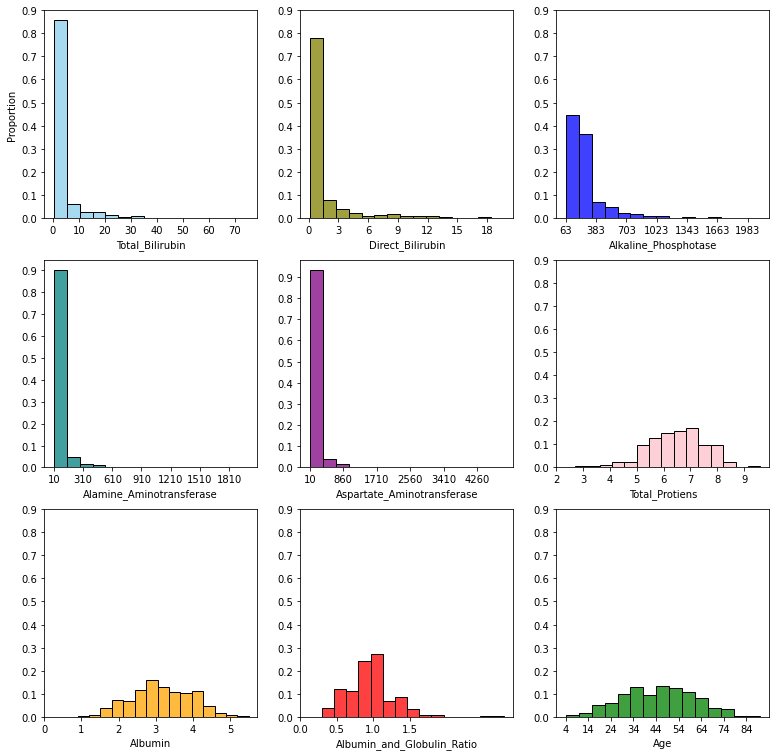
\includegraphics{output_125_0.png}
\caption{Histogramas variables cuantitativas}
\end{figure}

\clearpage

\textbf{Diagramas de barras para las variables categóricas}

Ahora vamos a realizar una serie de operaciones para generar dos
diagramas de barrras, uno para la variable Gender y otro para Diseased.

\begin{Shaded}
\begin{Highlighting}[]
\NormalTok{proportion\_Female }\OperatorTok{=} \BuiltInTok{len}\NormalTok{( Data\_Python.loc[ Data\_Python[}\StringTok{\textquotesingle{}Gender\textquotesingle{}}\NormalTok{]}\OperatorTok{==}\DecValTok{0}\NormalTok{ , :] ) }\OperatorTok{/} \BuiltInTok{len}\NormalTok{(Data\_Python)}
\NormalTok{proportion\_Male }\OperatorTok{=} \BuiltInTok{len}\NormalTok{( Data\_Python.loc[ Data\_Python[}\StringTok{\textquotesingle{}Gender\textquotesingle{}}\NormalTok{]}\OperatorTok{==}\DecValTok{1}\NormalTok{ , :] ) }\OperatorTok{/} \BuiltInTok{len}\NormalTok{(Data\_Python)}

\NormalTok{proportion\_Diseased\_yes }\OperatorTok{=} \BuiltInTok{len}\NormalTok{( Data\_Python.loc[ Data\_Python[}\StringTok{\textquotesingle{}Diseased\textquotesingle{}}\NormalTok{]}\OperatorTok{==}\DecValTok{0}\NormalTok{ , :] ) }\OperatorTok{/} \BuiltInTok{len}\NormalTok{(Data\_Python)}
\NormalTok{proportion\_Diseased\_no }\OperatorTok{=} \BuiltInTok{len}\NormalTok{( Data\_Python.loc[ Data\_Python[}\StringTok{\textquotesingle{}Diseased\textquotesingle{}}\NormalTok{]}\OperatorTok{==}\DecValTok{1}\NormalTok{ , :] ) }\OperatorTok{/} \BuiltInTok{len}\NormalTok{(Data\_Python)}
\end{Highlighting}
\end{Shaded}

\begin{Shaded}
\begin{Highlighting}[]
\NormalTok{Data\_Python[}\StringTok{\textquotesingle{}proportion\_Gender\textquotesingle{}}\NormalTok{] }\OperatorTok{=} \DecValTok{0}


\ControlFlowTok{for}\NormalTok{ i }\KeywordTok{in} \BuiltInTok{range}\NormalTok{(}\DecValTok{0}\NormalTok{, }\BuiltInTok{len}\NormalTok{(Data\_Python)):}

    \ControlFlowTok{if}\NormalTok{ Data\_Python[}\StringTok{\textquotesingle{}Gender\textquotesingle{}}\NormalTok{][i] }\OperatorTok{==} \DecValTok{0}\NormalTok{ :}

\NormalTok{        Data\_Python[}\StringTok{\textquotesingle{}proportion\_Gender\textquotesingle{}}\NormalTok{][i] }\OperatorTok{=}\NormalTok{ proportion\_Female}

    \ControlFlowTok{else}\NormalTok{ :}

\NormalTok{        Data\_Python[}\StringTok{\textquotesingle{}proportion\_Gender\textquotesingle{}}\NormalTok{][i] }\OperatorTok{=}\NormalTok{ proportion\_Male}
\end{Highlighting}
\end{Shaded}

\begin{Shaded}
\begin{Highlighting}[]
\NormalTok{Data\_Python[}\StringTok{\textquotesingle{}proportion\_Diseased\textquotesingle{}}\NormalTok{] }\OperatorTok{=} \DecValTok{0}


\ControlFlowTok{for}\NormalTok{ i }\KeywordTok{in} \BuiltInTok{range}\NormalTok{(}\DecValTok{0}\NormalTok{, }\BuiltInTok{len}\NormalTok{(Data\_Python)):}

    \ControlFlowTok{if}\NormalTok{ Data\_Python[}\StringTok{\textquotesingle{}Diseased\textquotesingle{}}\NormalTok{][i] }\OperatorTok{==} \DecValTok{0}\NormalTok{ :}

\NormalTok{        Data\_Python[}\StringTok{\textquotesingle{}proportion\_Diseased\textquotesingle{}}\NormalTok{][i] }\OperatorTok{=}\NormalTok{ proportion\_Diseased\_yes}

    \ControlFlowTok{else}\NormalTok{ :}

\NormalTok{        Data\_Python[}\StringTok{\textquotesingle{}proportion\_Diseased\textquotesingle{}}\NormalTok{][i] }\OperatorTok{=}\NormalTok{ proportion\_Diseased\_no}
\end{Highlighting}
\end{Shaded}

\begin{Shaded}
\begin{Highlighting}[]
\NormalTok{fig, axs }\OperatorTok{=}\NormalTok{ plt.subplots(}\DecValTok{1}\NormalTok{, }\DecValTok{2}\NormalTok{, figsize}\OperatorTok{=}\NormalTok{(}\DecValTok{8}\NormalTok{, }\DecValTok{8}\NormalTok{))}

\NormalTok{p1 }\OperatorTok{=}\NormalTok{ sns.barplot(x}\OperatorTok{=}\StringTok{\textquotesingle{}Gender\textquotesingle{}}\NormalTok{, y}\OperatorTok{=}\StringTok{\textquotesingle{}proportion\_Gender\textquotesingle{}}\NormalTok{, data}\OperatorTok{=}\NormalTok{Data\_Python, ax}\OperatorTok{=}\NormalTok{axs[}\DecValTok{0}\NormalTok{]) }
\NormalTok{p1.set\_yticks( np.arange(}\DecValTok{0}\NormalTok{, }\FloatTok{0.85}\NormalTok{, }\FloatTok{0.1}\NormalTok{)  )}
\NormalTok{p1.set\_xticklabels([}\StringTok{\textquotesingle{}Female\textquotesingle{}}\NormalTok{, }\StringTok{\textquotesingle{}Male\textquotesingle{}}\NormalTok{])}
\NormalTok{p1.axes.}\BuiltInTok{set}\NormalTok{(xlabel}\OperatorTok{=}\StringTok{\textquotesingle{}Gender\textquotesingle{}}\NormalTok{, ylabel}\OperatorTok{=}\StringTok{\textquotesingle{}proportion\textquotesingle{}}\NormalTok{)}

\NormalTok{p2 }\OperatorTok{=}\NormalTok{ sns.barplot(x}\OperatorTok{=}\StringTok{\textquotesingle{}Diseased\textquotesingle{}}\NormalTok{, y}\OperatorTok{=}\StringTok{\textquotesingle{}proportion\_Diseased\textquotesingle{}}\NormalTok{, data}\OperatorTok{=}\NormalTok{Data\_Python, ax}\OperatorTok{=}\NormalTok{axs[}\DecValTok{1}\NormalTok{]) }
\NormalTok{p2.set\_yticks( np.arange(}\DecValTok{0}\NormalTok{, }\FloatTok{0.85}\NormalTok{, }\FloatTok{0.1}\NormalTok{)  )}
\NormalTok{p2.set\_xticklabels([}\StringTok{\textquotesingle{}Yes\textquotesingle{}}\NormalTok{, }\StringTok{\textquotesingle{}No\textquotesingle{}}\NormalTok{])}
\NormalTok{p2.axes.}\BuiltInTok{set}\NormalTok{(xlabel}\OperatorTok{=}\StringTok{\textquotesingle{}Diseased\textquotesingle{}}\NormalTok{, ylabel}\OperatorTok{=}\StringTok{\textquotesingle{} \textquotesingle{}}\NormalTok{)}

\NormalTok{plt.show()}
\end{Highlighting}
\end{Shaded}

\begin{figure}
\centering
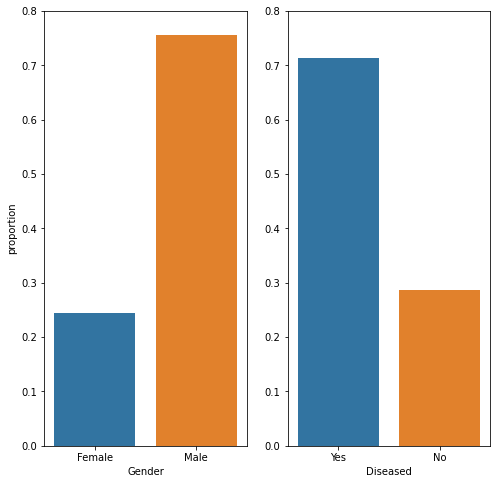
\includegraphics[width=5.20833in,height=4.16667in]{output_133_0.png}
\caption{Diagramas de barras variables categoricas}
\end{figure}

\begin{Shaded}
\begin{Highlighting}[]
\NormalTok{[ proportion\_Female , proportion\_Male ]}
\end{Highlighting}
\end{Shaded}

\begin{verbatim}
[0.24356775300171526, 0.7564322469982847]
\end{verbatim}

\begin{Shaded}
\begin{Highlighting}[]
\NormalTok{[ proportion\_Diseased\_yes , proportion\_Diseased\_no ]}
\end{Highlighting}
\end{Shaded}

\begin{verbatim}
[0.7135506003430532, 0.2864493996569468]
\end{verbatim}

Como puede verse el porcentaje de mujeres en la muestra es del 24.36\% ,
mientras que el de hombres es del 75.64\%

Por otro lado el porcentaje de endfermos es del71.36\%, mientras que el
de no enfermos es del 28.64\%

\newpage

\hypertarget{box-plots-para-las-variables-cuantitativas}{%
\subsubsection{\texorpdfstring{Box-plots para las variables
cuantitativas
}{Box-plots para las variables cuantitativas }}\label{box-plots-para-las-variables-cuantitativas}}

\begin{Shaded}
\begin{Highlighting}[]
\NormalTok{fig, axs }\OperatorTok{=}\NormalTok{ plt.subplots(}\DecValTok{3}\NormalTok{, }\DecValTok{3}\NormalTok{, figsize}\OperatorTok{=}\NormalTok{(}\DecValTok{13}\NormalTok{, }\DecValTok{13}\NormalTok{))}

\NormalTok{p1 }\OperatorTok{=}\NormalTok{ sns.boxplot(x}\OperatorTok{=}\NormalTok{Data\_Python[}\StringTok{\textquotesingle{}Age\textquotesingle{}}\NormalTok{], color}\OperatorTok{=}\StringTok{"palegreen"}\NormalTok{, ax}\OperatorTok{=}\NormalTok{axs[}\DecValTok{0}\NormalTok{, }\DecValTok{0}\NormalTok{])}
\NormalTok{p1.set\_xticks( }\BuiltInTok{range}\NormalTok{(}\BuiltInTok{int}\NormalTok{(Data\_Python[}\StringTok{\textquotesingle{}Age\textquotesingle{}}\NormalTok{].}\BuiltInTok{min}\NormalTok{()) , }\BuiltInTok{int}\NormalTok{(Data\_Python[}\StringTok{\textquotesingle{}Age\textquotesingle{}}\NormalTok{].}\BuiltInTok{max}\NormalTok{()}\OperatorTok{+}\DecValTok{10}\NormalTok{) , }\DecValTok{10}\NormalTok{) )}

\NormalTok{p2 }\OperatorTok{=}\NormalTok{ sns.boxplot(x}\OperatorTok{=}\NormalTok{Data\_Python[}\StringTok{\textquotesingle{}Direct\_Bilirubin\textquotesingle{}}\NormalTok{], color}\OperatorTok{=}\StringTok{"olive"}\NormalTok{, ax}\OperatorTok{=}\NormalTok{axs[}\DecValTok{0}\NormalTok{, }\DecValTok{1}\NormalTok{])}
\NormalTok{p2.set\_xticks( }\BuiltInTok{range}\NormalTok{(}\BuiltInTok{int}\NormalTok{(Data\_Python[}\StringTok{\textquotesingle{}Direct\_Bilirubin\textquotesingle{}}\NormalTok{].}\BuiltInTok{min}\NormalTok{()) , }\BuiltInTok{int}\NormalTok{(Data\_Python[}\StringTok{\textquotesingle{}Direct\_Bilirubin\textquotesingle{}}\NormalTok{].}\BuiltInTok{max}\NormalTok{()) , }\DecValTok{10}\NormalTok{) )}

\NormalTok{p3 }\OperatorTok{=}\NormalTok{ sns.boxplot(x}\OperatorTok{=}\NormalTok{Data\_Python[}\StringTok{\textquotesingle{}Alkaline\_Phosphotase\textquotesingle{}}\NormalTok{], color}\OperatorTok{=}\StringTok{"blue"}\NormalTok{, ax}\OperatorTok{=}\NormalTok{axs[}\DecValTok{1}\NormalTok{, }\DecValTok{0}\NormalTok{])}
\NormalTok{p3.set\_xticks( }\BuiltInTok{range}\NormalTok{(}\BuiltInTok{int}\NormalTok{(Data\_Python[}\StringTok{\textquotesingle{}Alkaline\_Phosphotase\textquotesingle{}}\NormalTok{].}\BuiltInTok{min}\NormalTok{()) , }\BuiltInTok{int}\NormalTok{(Data\_Python[}\StringTok{\textquotesingle{}Alkaline\_Phosphotase\textquotesingle{}}\NormalTok{].}\BuiltInTok{max}\NormalTok{() ) , }\DecValTok{300}\NormalTok{) )}

\NormalTok{p4 }\OperatorTok{=}\NormalTok{ sns.boxplot(x}\OperatorTok{=}\NormalTok{Data\_Python[}\StringTok{\textquotesingle{}Alamine\_Aminotransferase\textquotesingle{}}\NormalTok{], color}\OperatorTok{=}\StringTok{"teal"}\NormalTok{, ax}\OperatorTok{=}\NormalTok{axs[}\DecValTok{1}\NormalTok{, }\DecValTok{1}\NormalTok{])}
\NormalTok{p4.set\_xticks( }\BuiltInTok{range}\NormalTok{(}\BuiltInTok{int}\NormalTok{(Data\_Python[}\StringTok{\textquotesingle{}Alamine\_Aminotransferase\textquotesingle{}}\NormalTok{].}\BuiltInTok{min}\NormalTok{()) , }\BuiltInTok{int}\NormalTok{(Data\_Python[}\StringTok{\textquotesingle{}Alamine\_Aminotransferase\textquotesingle{}}\NormalTok{].}\BuiltInTok{max}\NormalTok{()) , }\DecValTok{500}\NormalTok{) )}

\NormalTok{p5 }\OperatorTok{=}\NormalTok{ sns.boxplot(x}\OperatorTok{=}\NormalTok{Data\_Python[}\StringTok{\textquotesingle{}Aspartate\_Aminotransferase\textquotesingle{}}\NormalTok{], color}\OperatorTok{=}\StringTok{"purple"}\NormalTok{, ax}\OperatorTok{=}\NormalTok{axs[}\DecValTok{0}\NormalTok{, }\DecValTok{2}\NormalTok{])}
\NormalTok{p5.set\_xticks( }\BuiltInTok{range}\NormalTok{(}\BuiltInTok{int}\NormalTok{(Data\_Python[}\StringTok{\textquotesingle{}Aspartate\_Aminotransferase\textquotesingle{}}\NormalTok{].}\BuiltInTok{min}\NormalTok{()) , }\BuiltInTok{int}\NormalTok{(Data\_Python[}\StringTok{\textquotesingle{}Aspartate\_Aminotransferase\textquotesingle{}}\NormalTok{].}\BuiltInTok{max}\NormalTok{()) , }\DecValTok{850}\NormalTok{) )}

\NormalTok{p6 }\OperatorTok{=}\NormalTok{ sns.boxplot(x}\OperatorTok{=}\NormalTok{Data\_Python[}\StringTok{\textquotesingle{}Total\_Protiens\textquotesingle{}}\NormalTok{], color}\OperatorTok{=}\StringTok{"pink"}\NormalTok{, ax}\OperatorTok{=}\NormalTok{axs[}\DecValTok{1}\NormalTok{, }\DecValTok{2}\NormalTok{])}
\NormalTok{p6.set\_xticks( }\BuiltInTok{range}\NormalTok{(}\BuiltInTok{int}\NormalTok{(Data\_Python[}\StringTok{\textquotesingle{}Total\_Protiens\textquotesingle{}}\NormalTok{].}\BuiltInTok{min}\NormalTok{()) , }\BuiltInTok{int}\NormalTok{(Data\_Python[}\StringTok{\textquotesingle{}Total\_Protiens\textquotesingle{}}\NormalTok{].}\BuiltInTok{max}\NormalTok{()) , }\DecValTok{10}\NormalTok{) )}

\NormalTok{p7 }\OperatorTok{=}\NormalTok{ sns.boxplot(x}\OperatorTok{=}\NormalTok{Data\_Python[}\StringTok{\textquotesingle{}Albumin\textquotesingle{}}\NormalTok{], color}\OperatorTok{=}\StringTok{"orange"}\NormalTok{, ax}\OperatorTok{=}\NormalTok{axs[}\DecValTok{2}\NormalTok{, }\DecValTok{2}\NormalTok{])}
\NormalTok{p7.set\_xticks( }\BuiltInTok{range}\NormalTok{(}\BuiltInTok{int}\NormalTok{(Data\_Python[}\StringTok{\textquotesingle{}Albumin\textquotesingle{}}\NormalTok{].}\BuiltInTok{min}\NormalTok{()) , }\BuiltInTok{int}\NormalTok{(Data\_Python[}\StringTok{\textquotesingle{}Albumin\textquotesingle{}}\NormalTok{].}\BuiltInTok{max}\NormalTok{()) , }\DecValTok{10}\NormalTok{) )}

\NormalTok{p8 }\OperatorTok{=}\NormalTok{ sns.boxplot(x}\OperatorTok{=}\NormalTok{Data\_Python[}\StringTok{\textquotesingle{}Albumin\_and\_Globulin\_Ratio\textquotesingle{}}\NormalTok{], color}\OperatorTok{=}\StringTok{"red"}\NormalTok{, ax}\OperatorTok{=}\NormalTok{axs[}\DecValTok{2}\NormalTok{, }\DecValTok{1}\NormalTok{])}
\NormalTok{p8.set\_xticks( }\BuiltInTok{range}\NormalTok{(}\BuiltInTok{int}\NormalTok{(Data\_Python[}\StringTok{\textquotesingle{}Albumin\_and\_Globulin\_Ratio\textquotesingle{}}\NormalTok{].}\BuiltInTok{min}\NormalTok{()) , }\BuiltInTok{int}\NormalTok{(Data\_Python[}\StringTok{\textquotesingle{}Albumin\_and\_Globulin\_Ratio\textquotesingle{}}\NormalTok{].}\BuiltInTok{max}\NormalTok{()) , }\DecValTok{10}\NormalTok{) )}

\NormalTok{p9 }\OperatorTok{=}\NormalTok{ sns.boxplot(x}\OperatorTok{=}\NormalTok{Data\_Python[}\StringTok{\textquotesingle{}Total\_Bilirubin\textquotesingle{}}\NormalTok{], color}\OperatorTok{=}\StringTok{"skyblue"}\NormalTok{, ax}\OperatorTok{=}\NormalTok{axs[}\DecValTok{2}\NormalTok{, }\DecValTok{0}\NormalTok{])}
\NormalTok{p9.set\_xticks( }\BuiltInTok{range}\NormalTok{(}\BuiltInTok{int}\NormalTok{(Data\_Python[}\StringTok{\textquotesingle{}Total\_Bilirubin\textquotesingle{}}\NormalTok{].}\BuiltInTok{min}\NormalTok{()) , }\BuiltInTok{int}\NormalTok{(Data\_Python[}\StringTok{\textquotesingle{}Total\_Bilirubin\textquotesingle{}}\NormalTok{].}\BuiltInTok{max}\NormalTok{()) , }\DecValTok{10}\NormalTok{) )}


\NormalTok{plt.show()}
\end{Highlighting}
\end{Shaded}

\begin{figure}
\centering
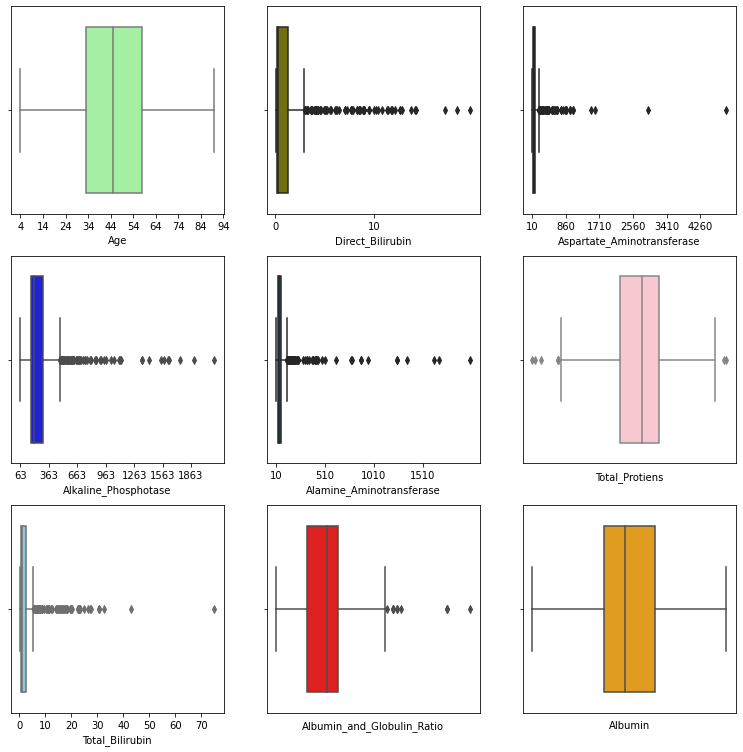
\includegraphics{output_140_0.png}
\caption{Box-plots variables cuantitativas}
\end{figure}

\newpage

\hypertarget{anuxe1lisis-de-la-relaciuxf3n-entre-los-predictores-categoricos-y-la-respuesta}{%
\subsubsection{\texorpdfstring{Análisis de la relación entre los
predictores categoricos y la respuesta
}{Análisis de la relación entre los predictores categoricos y la respuesta }}\label{anuxe1lisis-de-la-relaciuxf3n-entre-los-predictores-categoricos-y-la-respuesta}}

\textbf{Analisis relación entre respuesta (Diseased) y Gender}

\vspace{0.55cm}

\textbf{Frecuencia relativa de genero condicionada a enfermedad}

Ahora vamos a realizar una serie de operaciones para obtener una tabla
de frecuencias relativas de la variable Gender condicionada a la
respuesta (Diseased). También obtendremos el gráfico de barras asociado
a esta tabla.

\begin{Shaded}
\begin{Highlighting}[]
\NormalTok{Df\_Diseased\_Yes }\OperatorTok{=}\NormalTok{ Data\_Python.loc[ Data\_Python[}\StringTok{\textquotesingle{}Diseased\textquotesingle{}}\NormalTok{]}\OperatorTok{==}\DecValTok{0}\NormalTok{ , :] }

\NormalTok{proportion\_Female\_in\_Diseased\_Yes }\OperatorTok{=} \BuiltInTok{len}\NormalTok{( Df\_Diseased\_Yes.loc[Df\_Diseased\_Yes[}\StringTok{\textquotesingle{}Gender\textquotesingle{}}\NormalTok{]}\OperatorTok{==}\DecValTok{0}\NormalTok{ , :] ) }\OperatorTok{/} \BuiltInTok{len}\NormalTok{(Df\_Diseased\_Yes)}

\CommentTok{\#\#\#\#\#\#\#\#\#\#\#\#\#\#\#\#\#\#\#\#}

\NormalTok{Df\_Diseased\_Yes }\OperatorTok{=}\NormalTok{ Data\_Python.loc[ Data\_Python[}\StringTok{\textquotesingle{}Diseased\textquotesingle{}}\NormalTok{]}\OperatorTok{==}\DecValTok{0}\NormalTok{ , :] }

\NormalTok{proportion\_Male\_in\_Diseased\_Yes }\OperatorTok{=} \BuiltInTok{len}\NormalTok{( Df\_Diseased\_Yes.loc[Df\_Diseased\_Yes[}\StringTok{\textquotesingle{}Gender\textquotesingle{}}\NormalTok{]}\OperatorTok{==}\DecValTok{1}\NormalTok{ , :] ) }\OperatorTok{/} \BuiltInTok{len}\NormalTok{(Df\_Diseased\_Yes)}

\CommentTok{\#\#\#\#\#\#\#\#\#\#\#\#\#\#\#\#\#\#\#\#}

\NormalTok{Df\_Diseased\_No }\OperatorTok{=}\NormalTok{ Data\_Python.loc[ Data\_Python[}\StringTok{\textquotesingle{}Diseased\textquotesingle{}}\NormalTok{]}\OperatorTok{==}\DecValTok{1}\NormalTok{ , :] }

\NormalTok{proportion\_Female\_in\_Diseased\_No }\OperatorTok{=} \BuiltInTok{len}\NormalTok{( Df\_Diseased\_No.loc[Df\_Diseased\_No[}\StringTok{\textquotesingle{}Gender\textquotesingle{}}\NormalTok{]}\OperatorTok{==}\DecValTok{0}\NormalTok{ , :] ) }\OperatorTok{/} \BuiltInTok{len}\NormalTok{(Df\_Diseased\_No)}

\CommentTok{\#\#\#\#\#\#\#\#\#\#\#\#\#\#\#\#\#\#\#\#}

\NormalTok{Df\_Diseased\_No }\OperatorTok{=}\NormalTok{ Data\_Python.loc[ Data\_Python[}\StringTok{\textquotesingle{}Diseased\textquotesingle{}}\NormalTok{]}\OperatorTok{==}\DecValTok{1}\NormalTok{ , :] }

\NormalTok{proportion\_Male\_in\_Diseased\_No }\OperatorTok{=} \BuiltInTok{len}\NormalTok{( Df\_Diseased\_No.loc[Df\_Diseased\_No[}\StringTok{\textquotesingle{}Gender\textquotesingle{}}\NormalTok{]}\OperatorTok{==}\DecValTok{1}\NormalTok{ , :] ) }\OperatorTok{/} \BuiltInTok{len}\NormalTok{(Df\_Diseased\_No)}
\end{Highlighting}
\end{Shaded}

Función para calcular tablas de frecuencias relativas condicionadas con
dos variables:

\begin{Shaded}
\begin{Highlighting}[]
\KeywordTok{def}\NormalTok{ Table\_Con\_Rel\_Freq\_2\_Var\_Py (df, var1, p1, p2, var1\_name}\OperatorTok{=}\StringTok{\textquotesingle{}var1\textquotesingle{}}\NormalTok{ , var2\_name}\OperatorTok{=}\StringTok{\textquotesingle{}var2\textquotesingle{}}\NormalTok{) :}

\NormalTok{    table }\OperatorTok{=}\NormalTok{ np.zeros(( p2}\OperatorTok{+}\DecValTok{1}\NormalTok{ , p1}\OperatorTok{+}\DecValTok{1}\NormalTok{ ))}
\NormalTok{    table[:] }\OperatorTok{=}\NormalTok{ np.nan}

\CommentTok{\#\#\#\#\#\#\#\#\#\#\#\#\#\#\#\#\#\#\#\#\#\#\#\#\#\#\#\#\#\#\#\#\#\#\#\#\#\#\#\#\#\#\#\#\#\#\#\#\#\#\#\#\#\#\#\#\#\#}

    \ControlFlowTok{for}\NormalTok{ i }\KeywordTok{in} \BuiltInTok{range}\NormalTok{(}\DecValTok{0}\NormalTok{, p2}\OperatorTok{+}\DecValTok{1}\NormalTok{):}
        \ControlFlowTok{for}\NormalTok{ j }\KeywordTok{in} \BuiltInTok{range}\NormalTok{(}\DecValTok{0}\NormalTok{, p1}\OperatorTok{+}\DecValTok{1}\NormalTok{):}

\NormalTok{            df\_new }\OperatorTok{=}\NormalTok{ df.loc[ var1 }\OperatorTok{==}\NormalTok{ j   , : ]}

\NormalTok{            table[i,j] }\OperatorTok{=} \BuiltInTok{len}\NormalTok{( df\_new.loc[ df\_new[var2\_name] }\OperatorTok{==}\NormalTok{ i , :] ) }\OperatorTok{/} \BuiltInTok{len}\NormalTok{(df\_new)}
    
\NormalTok{    table }\OperatorTok{=}\NormalTok{ pd.DataFrame(table)}

    \ControlFlowTok{return}\NormalTok{ table}
\end{Highlighting}
\end{Shaded}

\begin{Shaded}
\begin{Highlighting}[]
\NormalTok{Frec\_Relativas\_Condicionadas\_Gender\_in\_Diseased }\OperatorTok{=}\NormalTok{ Table\_Con\_Rel\_Freq\_2\_Var\_Py (Data\_Python, Data\_Python[}\StringTok{\textquotesingle{}Diseased\textquotesingle{}}\NormalTok{], }\DecValTok{1}\NormalTok{, }\DecValTok{1}\NormalTok{, var1\_name}\OperatorTok{=}\StringTok{\textquotesingle{}Diseased\textquotesingle{}}\NormalTok{ , var2\_name}\OperatorTok{=}\StringTok{\textquotesingle{}Gender\textquotesingle{}}\NormalTok{)}

\NormalTok{Frec\_Relativas\_Condicionadas\_Gender\_in\_Diseased.index }\OperatorTok{=}\NormalTok{ [}\StringTok{\textquotesingle{}Female\textquotesingle{}}\NormalTok{ , }\StringTok{\textquotesingle{}Male\textquotesingle{}}\NormalTok{]}
\NormalTok{Frec\_Relativas\_Condicionadas\_Gender\_in\_Diseased.columns }\OperatorTok{=}\NormalTok{ [}\StringTok{\textquotesingle{}Yes\textquotesingle{}}\NormalTok{ , }\StringTok{\textquotesingle{}No\textquotesingle{}}\NormalTok{]}
\NormalTok{Frec\_Relativas\_Condicionadas\_Gender\_in\_Diseased }\OperatorTok{=}\NormalTok{ Frec\_Relativas\_Condicionadas\_Gender\_in\_Diseased.style.set\_caption(}\StringTok{"Gender  |  Diseased "}\NormalTok{)}
\end{Highlighting}
\end{Shaded}

\begin{Shaded}
\begin{Highlighting}[]
\NormalTok{p1 }\OperatorTok{=}\NormalTok{ sns.countplot(data}\OperatorTok{=}\NormalTok{Data\_Python, x}\OperatorTok{=}\StringTok{"Diseased"}\NormalTok{, hue}\OperatorTok{=}\StringTok{"Gender"}\NormalTok{, palette}\OperatorTok{=}\StringTok{"husl"}\NormalTok{)}
\NormalTok{p1.set\_xticklabels([}\StringTok{\textquotesingle{}Yes\textquotesingle{}}\NormalTok{, }\StringTok{\textquotesingle{}No\textquotesingle{}}\NormalTok{])}
\NormalTok{p1.legend(title}\OperatorTok{=}\StringTok{\textquotesingle{}Gender\textquotesingle{}}\NormalTok{, loc}\OperatorTok{=}\StringTok{\textquotesingle{}upper right\textquotesingle{}}\NormalTok{, labels}\OperatorTok{=}\NormalTok{[}\StringTok{\textquotesingle{}Female\textquotesingle{}}\NormalTok{, }\StringTok{\textquotesingle{}Male\textquotesingle{}}\NormalTok{])}
\end{Highlighting}
\end{Shaded}

\begin{figure}
\centering
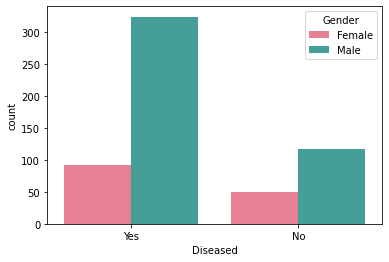
\includegraphics[width=4.375in,height=3.33333in]{output_152_1.png}
\caption{Diagrama de barras de Gender condicionada a Diseased}
\end{figure}

\newpage

\begin{Shaded}
\begin{Highlighting}[]
\NormalTok{Frec\_Relativas\_Condicionadas\_Gender\_in\_Diseased}
\end{Highlighting}
\end{Shaded}

\begin{verbatim}
Gender | Diseased
                
            Yes         No
Female      0.221154    0.299401
Male        0.778846    0.700599
\end{verbatim}

\begin{Shaded}
\begin{Highlighting}[]
\NormalTok{[proportion\_Female\_in\_Diseased\_Yes , proportion\_Male\_in\_Diseased\_Yes]}
\end{Highlighting}
\end{Shaded}

\begin{verbatim}
[0.22115384615384615, 0.7788461538461539]
\end{verbatim}

\begin{Shaded}
\begin{Highlighting}[]
\NormalTok{[proportion\_Female\_in\_Diseased\_No , proportion\_Male\_in\_Diseased\_No]}
\end{Highlighting}
\end{Shaded}

\begin{verbatim}
[0.2994011976047904, 0.7005988023952096]
\end{verbatim}

Como puede observarse el porcentaje de mujeres dentro del grupo de los
enfermos es del 22.12\% , mientras que el de hombres es del 77.88\%.

Por otro lado el porcentaje de mujeres dentro del grupo de los no
enfermos es del 29.94\%, mientras que el de hombres es del 70.06\%

\vspace{0.5cm}

\textbf{Frecuencia relativa de enfermedad condicionada al genero}

Ahora vamos a realizar una serie de operaciones para obtener una tabla
de frecuencias relativas de la variable respuesta (Diseased)
condicionada a la variable Gender . También obtendremos el gráfico de
barras asociado a esta tabla.

\begin{Shaded}
\begin{Highlighting}[]
\NormalTok{Frec\_Relativas\_Condicionadas\_Diseased\_in\_Gender }\OperatorTok{=}\NormalTok{ Table\_Con\_Rel\_Freq\_2\_Var\_Py (Data\_Python, Data\_Python[}\StringTok{\textquotesingle{}Gender\textquotesingle{}}\NormalTok{], }\DecValTok{1}\NormalTok{, }\DecValTok{1}\NormalTok{, var1\_name}\OperatorTok{=}\StringTok{\textquotesingle{}Gender\textquotesingle{}}\NormalTok{ , var2\_name}\OperatorTok{=}\StringTok{\textquotesingle{}Diseased\textquotesingle{}}\NormalTok{)}
\NormalTok{Frec\_Relativas\_Condicionadas\_Diseased\_in\_Gender.index }\OperatorTok{=}\NormalTok{ [}\StringTok{\textquotesingle{}Yes\textquotesingle{}}\NormalTok{ , }\StringTok{\textquotesingle{}No\textquotesingle{}}\NormalTok{]}
\NormalTok{Frec\_Relativas\_Condicionadas\_Diseased\_in\_Gender.columns }\OperatorTok{=}\NormalTok{ [}\StringTok{\textquotesingle{}Female\textquotesingle{}}\NormalTok{ , }\StringTok{\textquotesingle{}Male\textquotesingle{}}\NormalTok{]}
\NormalTok{Frec\_Relativas\_Condicionadas\_Diseased\_in\_Gender }\OperatorTok{=}\NormalTok{ Frec\_Relativas\_Condicionadas\_Diseased\_in\_Gender.style.set\_caption(}\StringTok{"Diseased | Gender"}\NormalTok{)}
\end{Highlighting}
\end{Shaded}

\begin{Shaded}
\begin{Highlighting}[]
\NormalTok{p }\OperatorTok{=}\NormalTok{ sns.countplot(data}\OperatorTok{=}\NormalTok{Data\_Python, x}\OperatorTok{=}\StringTok{"Gender"}\NormalTok{, hue}\OperatorTok{=}\StringTok{"Diseased"}\NormalTok{, palette}\OperatorTok{=}\StringTok{"husl"}\NormalTok{)}
\NormalTok{p.set\_xticklabels([}\StringTok{\textquotesingle{}Female\textquotesingle{}}\NormalTok{, }\StringTok{\textquotesingle{}Male\textquotesingle{}}\NormalTok{])}
\NormalTok{p.legend(title}\OperatorTok{=}\StringTok{\textquotesingle{}Diseased\textquotesingle{}}\NormalTok{, loc}\OperatorTok{=}\StringTok{\textquotesingle{}upper right\textquotesingle{}}\NormalTok{, labels}\OperatorTok{=}\NormalTok{[}\StringTok{\textquotesingle{}Yes\textquotesingle{}}\NormalTok{, }\StringTok{\textquotesingle{}No\textquotesingle{}}\NormalTok{])}
\end{Highlighting}
\end{Shaded}

\begin{figure}
\centering
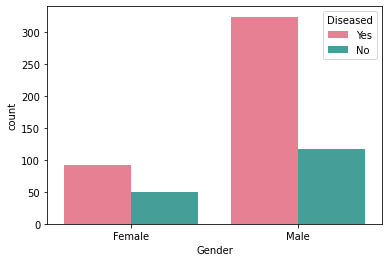
\includegraphics[width=4.375in,height=3.33333in]{output_162_1.png}
\caption{Diagrama de barras de Diseased condicionada a Gender}
\end{figure}

\begin{Shaded}
\begin{Highlighting}[]
\NormalTok{Frec\_Relativas\_Condicionadas\_Diseased\_in\_Gender}
\end{Highlighting}
\end{Shaded}

\begin{verbatim}
Diseased | Gender
    
      Female      Male
Yes 0.647887    0.734694
No  0.352113    0.265306
\end{verbatim}

Como puede observarse el porcentaje de enfermos dentro del grupo de as
mujeres es del 64.79\% , mientras que el de no enfermos es del 35.21\%.

Por otro lado el porcentaje de enfermos dentro del grupo de los hombres
es del 73.47\%, mientras que el de no enfermos es del 26.53\%

\newpage

\textbf{Analisis relación entre respuesta (Diseased) y Grupo de Edad}

\vspace{0.25cm}

\textbf{Frecuecnia relativa de enfermedad en funcion del grupo de edad}

Tenemos que categorizar la variable cuantitativa Age (edad) , para ello
debemos emplear una regla de categorización (mediana, media, cuartiles,
Scott \ldots)

Usaremos la regla de los cuartiles por simplicidad:

\begin{Shaded}
\begin{Highlighting}[]
\NormalTok{intervals }\OperatorTok{=}\NormalTok{ np.quantile( Data\_Python[}\StringTok{\textquotesingle{}Age\textquotesingle{}}\NormalTok{] , [}\DecValTok{0}\NormalTok{, }\FloatTok{0.25}\NormalTok{, }\FloatTok{0.5}\NormalTok{, }\FloatTok{0.75}\NormalTok{ , }\DecValTok{1}\NormalTok{])}
\NormalTok{intervals}
\end{Highlighting}
\end{Shaded}

\begin{verbatim}
array([ 4., 33., 45., 58., 90.])
\end{verbatim}

Nos apoyaremos en la funcion \texttt{cut()} de la libreria
\texttt{Pandas} para categorizar la variable Age usando la regla de los
cuartiles.

A esta función le das un vector (bins) y construye unos intervalos con
los elementos del vector, en este caso (3, 33{]}, (33, 45{]}, (45,
58{]}, (58, 90{]}. Luego te devuelve a qué intervalo pertenece cada
observación de una variable dada (en nuestro caso Age), y también nos
permite codificar estos intervalos con la codificacion estandar
(0,1,2,\ldots), y así obtener una nueva variable que es una versión
categorizada de la variable pasada (Age en nuestro caso).

Vamos a restar una cantidad positiva (por ejemplo 1) al mínimo de Age,
puesto que ese valor será el extremo inferior del primer intervalo, y
dicho intervalo será abierto en ese extremo (por configuración de la
función \texttt{cut}), por tanto si no restasemos una cantidad positiva,
el valor mínimo de Age no estaría en ninguno de los intervalos generados
por \texttt{cut()}

\begin{Shaded}
\begin{Highlighting}[]
\NormalTok{intervals[}\DecValTok{0}\NormalTok{] }\OperatorTok{=}\NormalTok{  intervals[}\DecValTok{0}\NormalTok{] }\OperatorTok{{-}} \DecValTok{1}

\NormalTok{intervals}
\end{Highlighting}
\end{Shaded}

\begin{verbatim}
array([ 3., 33., 45., 58., 90.])
\end{verbatim}

\begin{Shaded}
\begin{Highlighting}[]
\NormalTok{pd.cut(x}\OperatorTok{=}\NormalTok{Data\_Python[}\StringTok{\textquotesingle{}Age\textquotesingle{}}\NormalTok{] , bins}\OperatorTok{=}\NormalTok{intervals , right}\OperatorTok{=}\VariableTok{True}\NormalTok{)}
\end{Highlighting}
\end{Shaded}

\begin{verbatim}
0      (58.0, 90.0]
1      (58.0, 90.0]
2      (58.0, 90.0]
3      (45.0, 58.0]
4      (58.0, 90.0]
           ...     
578    (58.0, 90.0]
579    (33.0, 45.0]
580    (45.0, 58.0]
581     (3.0, 33.0]
582    (33.0, 45.0]
Name: Age, Length: 583, dtype: category
Categories (4, interval[float64, right]): [(3.0, 33.0] < (33.0, 45.0] < (45.0, 58.0] < (58.0, 90.0]]
\end{verbatim}

\begin{Shaded}
\begin{Highlighting}[]
\NormalTok{pd.cut(x}\OperatorTok{=}\NormalTok{Data\_Python[}\StringTok{\textquotesingle{}Age\textquotesingle{}}\NormalTok{] , bins}\OperatorTok{=}\NormalTok{intervals , labels}\OperatorTok{=}\VariableTok{False}\NormalTok{)}
\end{Highlighting}
\end{Shaded}

\begin{verbatim}
0      3
1      3
2      3
3      2
4      3
      ..
578    3
579    1
580    2
581    0
582    1
Name: Age, Length: 583, dtype: int64
\end{verbatim}

\vspace{0.1cm}

\begin{Shaded}
\begin{Highlighting}[]
\NormalTok{Data\_Python[}\StringTok{\textquotesingle{}Age\_cat\textquotesingle{}}\NormalTok{] }\OperatorTok{=}\NormalTok{ pd.cut(x}\OperatorTok{=}\NormalTok{Data\_Python[}\StringTok{\textquotesingle{}Age\textquotesingle{}}\NormalTok{] , bins}\OperatorTok{=}\NormalTok{intervals , labels}\OperatorTok{=}\VariableTok{False}\NormalTok{)}
\end{Highlighting}
\end{Shaded}

\vspace{0.2cm}

La nueva variable \(Age\_cat\) es tal que:

\[
Age\_cat_{i} = \left\lbrace\begin{array}{l} 0, \hspace{0.25cm} \text{ if $Age_{i} \in \left[ Min(Age ) \hspace{0.03cm} ,\hspace{0.03cm} Q(0.25, Age ) \right] $} \\ \\ 1, \hspace{0.25cm}\text{ if $Age_{i} \in ( Q(0.25 , Age ) , Q(0.50 , Age )] $}   
\\ \\ 2, \hspace{0.25cm} \text{ if $Age _{i} \in (Q(0.50 , Age ) , Q(0.75 , Age )] $}   \\ \\ 3,  \hspace{0.25cm} \text{ if $Age _{i} \in \left(Q(0.75 ,  Age ) \hspace{0.02cm},\hspace{0.02cm} Max(Age )\right] $} \end{array}\right.
\]

para \(\hspace{0.1cm} i=1,...,n\)

\vspace{0.2cm}

Ahora tenemos una variable que nos indica el grupo de edad de cada
individuo. Tenemos tes grupos de edad.

Grupo 0: \(\hspace{0.2cm} \leqslant 33\) años

Grupo 1: \(\hspace{0.2cm}\) entre \(33\) y \(45\) años

Grupo 2: \(\hspace{0.2cm}\) entre \(45\) y \(58\) años

grupo 3: \(\hspace{0.2cm}\) \(> 58\) años

\newpage

Ahora vamos a generar una tabla de frecuencias relativas de la variable
respuesta (Diseased) condicionada a la nueva variable Grupo de edad
(Age\_cat), también generaremos su gráfico de barras asociado.

\begin{Shaded}
\begin{Highlighting}[]
\NormalTok{Frec\_Relativas\_Condicionadas\_Diseased\_in\_Aged }\OperatorTok{=}\NormalTok{ Table\_Con\_Rel\_Freq\_2\_Var\_Py (Data\_Python, Data\_Python[}\StringTok{\textquotesingle{}Age\_cat\textquotesingle{}}\NormalTok{], }\DecValTok{3}\NormalTok{, }\DecValTok{1}\NormalTok{, var1\_name}\OperatorTok{=}\StringTok{\textquotesingle{}Age\_cat\textquotesingle{}}\NormalTok{ , var2\_name}\OperatorTok{=}\StringTok{\textquotesingle{}Diseased\textquotesingle{}}\NormalTok{)}
\NormalTok{Frec\_Relativas\_Condicionadas\_Diseased\_in\_Aged.index }\OperatorTok{=}\NormalTok{ [}\StringTok{\textquotesingle{}Yes\textquotesingle{}}\NormalTok{ , }\StringTok{\textquotesingle{}No\textquotesingle{}}\NormalTok{]}
\NormalTok{Frec\_Relativas\_Condicionadas\_Diseased\_in\_Aged.columns }\OperatorTok{=}\NormalTok{ [}\StringTok{\textquotesingle{}(3, 33]\textquotesingle{}}\NormalTok{, }\StringTok{\textquotesingle{}(33, 45]\textquotesingle{}}\NormalTok{ , }\StringTok{\textquotesingle{}(45, 58]\textquotesingle{}}\NormalTok{ , }\StringTok{\textquotesingle{}(58, 90]\textquotesingle{}}\NormalTok{]}
\NormalTok{Frec\_Relativas\_Condicionadas\_Diseased\_in\_Aged }\OperatorTok{=}\NormalTok{ Frec\_Relativas\_Condicionadas\_Diseased\_in\_Aged.style.set\_caption(}\StringTok{"Diseased | Age Group"}\NormalTok{)}
\end{Highlighting}
\end{Shaded}

\begin{Shaded}
\begin{Highlighting}[]
\NormalTok{p }\OperatorTok{=}\NormalTok{ sns.countplot(data}\OperatorTok{=}\NormalTok{Data\_Python, x}\OperatorTok{=}\StringTok{"Age\_cat"}\NormalTok{, hue}\OperatorTok{=}\StringTok{"Diseased"}\NormalTok{, palette}\OperatorTok{=}\StringTok{"husl"}\NormalTok{)}
\NormalTok{p.set\_xticklabels([}\StringTok{\textquotesingle{}(3, 33]\textquotesingle{}}\NormalTok{, }\StringTok{\textquotesingle{}(33, 45]\textquotesingle{}}\NormalTok{ , }\StringTok{\textquotesingle{}(45, 58]\textquotesingle{}}\NormalTok{ , }\StringTok{\textquotesingle{}(58, 90]\textquotesingle{}}\NormalTok{])}
\NormalTok{p.legend(title}\OperatorTok{=}\StringTok{\textquotesingle{}Diseased\textquotesingle{}}\NormalTok{, loc}\OperatorTok{=}\StringTok{\textquotesingle{}upper right\textquotesingle{}}\NormalTok{, labels}\OperatorTok{=}\NormalTok{[}\StringTok{\textquotesingle{}Yes\textquotesingle{}}\NormalTok{, }\StringTok{\textquotesingle{}No\textquotesingle{}}\NormalTok{] )}
\end{Highlighting}
\end{Shaded}

\begin{figure}
\centering
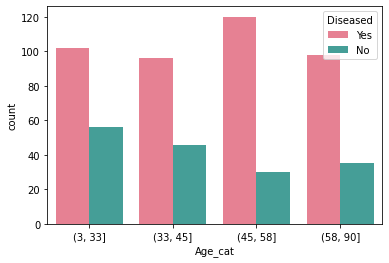
\includegraphics[width=4.375in,height=3.33333in]{output_187_1.png}
\caption{Grafico de barras de Diseased condicionada a grupo de edad
(Age\_cat)}
\end{figure}

\begin{Shaded}
\begin{Highlighting}[]
\NormalTok{Frec\_Relativas\_Condicionadas\_Diseased\_in\_Aged  }
\end{Highlighting}
\end{Shaded}

\begin{verbatim}
 Diseased | Age Group
 
        (3, 33]     (33, 45]     (45, 58]     (58, 90]
Yes     0.645570     0.676056     0.800000    0.736842
No      0.354430     0.323944     0.200000    0.263158
\end{verbatim}

\newpage

Como puede observarse dentro del grupo de los más jovenes (de edad menor
o igual a 33) el procentaje de enfermos es del 64.56\% , este porcentaje
aumenta hasta el 67.60\% en el grupo de individuos cuya edad esta entre
33 y 45 años, y hasta el 80\% en el de los individuos con una edad entre
45 y 58 años, luego pasa a ser del 73.68\% en el grupo de edad superior
a 58 años.

\vspace{1cm}

\textbf{Frecuecnia relativa de grupo de edad en funcion de enfermedad}

Ahora vamos a generar una tabla de frecuencias relativas de la variable
grupo de edad (Age\_cat) condicionada a la variable respuesta, también
generaremos su gráfico de barras asociado.

\begin{Shaded}
\begin{Highlighting}[]
\NormalTok{Frec\_Relativas\_Condicionadas\_Age\_in\_Diseased }\OperatorTok{=}\NormalTok{ Table\_Con\_Rel\_Freq\_2\_Var\_Py (Data\_Python, Data\_Python[}\StringTok{\textquotesingle{}Diseased\textquotesingle{}}\NormalTok{], }\DecValTok{1}\NormalTok{, }\DecValTok{3}\NormalTok{, var1\_name}\OperatorTok{=}\StringTok{\textquotesingle{}Diseased\textquotesingle{}}\NormalTok{ , var2\_name}\OperatorTok{=}\StringTok{\textquotesingle{}Age\_cat\textquotesingle{}}\NormalTok{)}
\NormalTok{Frec\_Relativas\_Condicionadas\_Age\_in\_Diseased.index }\OperatorTok{=}\NormalTok{ [}\StringTok{\textquotesingle{}(3, 33]\textquotesingle{}}\NormalTok{, }\StringTok{\textquotesingle{}(33, 45]\textquotesingle{}}\NormalTok{ , }\StringTok{\textquotesingle{}(45, 58]\textquotesingle{}}\NormalTok{ , }\StringTok{\textquotesingle{}(58, 90]\textquotesingle{}}\NormalTok{]}
\NormalTok{Frec\_Relativas\_Condicionadas\_Age\_in\_Diseased.columns }\OperatorTok{=}\NormalTok{ [}\StringTok{\textquotesingle{}Yes\textquotesingle{}}\NormalTok{ , }\StringTok{\textquotesingle{}No\textquotesingle{}}\NormalTok{]}
\NormalTok{Frec\_Relativas\_Condicionadas\_Age\_in\_Diseased }\OperatorTok{=}\NormalTok{ Frec\_Relativas\_Condicionadas\_Age\_in\_Diseased.style.set\_caption(}\StringTok{"Age Group | Diseased"}\NormalTok{)}
\end{Highlighting}
\end{Shaded}

\begin{Shaded}
\begin{Highlighting}[]
\NormalTok{p }\OperatorTok{=}\NormalTok{ sns.countplot(data}\OperatorTok{=}\NormalTok{Data\_Python, x}\OperatorTok{=}\StringTok{"Diseased"}\NormalTok{, hue}\OperatorTok{=}\StringTok{"Age\_cat"}\NormalTok{, palette}\OperatorTok{=}\StringTok{"husl"}\NormalTok{)}
\NormalTok{p.set\_xticklabels([}\StringTok{\textquotesingle{}Yes\textquotesingle{}}\NormalTok{, }\StringTok{\textquotesingle{}No\textquotesingle{}}\NormalTok{])}
\NormalTok{p.legend(title}\OperatorTok{=}\StringTok{\textquotesingle{}Group Age\textquotesingle{}}\NormalTok{, loc}\OperatorTok{=}\StringTok{\textquotesingle{}upper right\textquotesingle{}}\NormalTok{, labels}\OperatorTok{=}\NormalTok{ [}\StringTok{\textquotesingle{}(3, 33]\textquotesingle{}}\NormalTok{, }\StringTok{\textquotesingle{}(33, 45]\textquotesingle{}}\NormalTok{ , }\StringTok{\textquotesingle{}(45, 58]\textquotesingle{}}\NormalTok{ , }\StringTok{\textquotesingle{}(58, 90]\textquotesingle{}}\NormalTok{])}
\end{Highlighting}
\end{Shaded}

\begin{figure}
\centering
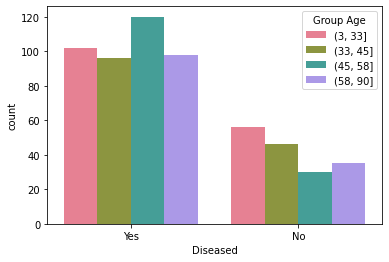
\includegraphics[width=4.375in,height=3.33333in]{output_195_1.png}
\caption{Grafico de barras de grupo de edad (Age\_cat) condicionada
Diseased}
\end{figure}

\begin{Shaded}
\begin{Highlighting}[]
\NormalTok{Frec\_Relativas\_Condicionadas\_Age\_in\_Diseased}
\end{Highlighting}
\end{Shaded}

\begin{verbatim}

Age Group | Diseased

                Yes          No
(3, 33]      0.245192     0.335329
(33, 45]     0.230769     0.275449
(45, 58]     0.288462     0.179641
(58, 90]     0.235577     0.209581
\end{verbatim}

Se puede apreciar que dentro del grupo de los enfermos , el grupo de
edad mas frecuente seria el de los individuos con una edad entre 45 y 58
años, seguido del de más de 58 años.

Por otro lado dentro del grupo de los no enfermos el grupo de edad
claramente mayoritario es el de los mas jovenes (edad menor o igual a 33
años), seguido del siguiente grupo mas joven (edad entre 33 y 45).

\vspace{1cm}

\hypertarget{anuxe1lisis-de-la-relaciuxf3n-entre-los-predictores-cuantitativos-y-la-respuesta}{%
\subsubsection{\texorpdfstring{4.3.5. Análisis de la relación entre los
predictores cuantitativos y la respuesta
}{4.3.5. Análisis de la relación entre los predictores cuantitativos y la respuesta }}\label{anuxe1lisis-de-la-relaciuxf3n-entre-los-predictores-cuantitativos-y-la-respuesta}}

\vspace{0.21cm}

\textbf{Resumen Estadístico Descriptivo Cuantitativo en función de
Diseased}

Ahora vamos a hacer una serie de operaciones para obtener una tabla en
la que se pueden comparar los valores de diferentes estadísticos
descriptivos básicos para cada variable cuantitativa en función del
valor de la respuesta (Diseased).

\begin{Shaded}
\begin{Highlighting}[]
\NormalTok{Data\_Python\_Quantitative\_Diseased\_yes }\OperatorTok{=}\NormalTok{ Data\_Python.loc[ Data\_Python[}\StringTok{\textquotesingle{}Diseased\textquotesingle{}}\NormalTok{] }\OperatorTok{==} \DecValTok{0}\NormalTok{ , (Data\_Python.columns }\OperatorTok{!=} \StringTok{\textquotesingle{}Gender\textquotesingle{}}\NormalTok{) }\OperatorTok{\&}\NormalTok{ (Data\_Python.columns }\OperatorTok{!=} \StringTok{\textquotesingle{}Diseased\textquotesingle{}}\NormalTok{) }\OperatorTok{\&}\NormalTok{ (Data\_Python.columns }\OperatorTok{!=} \StringTok{\textquotesingle{}proportion\_Gender\textquotesingle{}}\NormalTok{)  }\OperatorTok{\&}\NormalTok{ (Data\_Python.columns }\OperatorTok{!=} \StringTok{\textquotesingle{}proportion\_Diseased\textquotesingle{}}\NormalTok{) }\OperatorTok{\&}\NormalTok{ (Data\_Python.columns }\OperatorTok{!=} \StringTok{\textquotesingle{}Age\_cat\textquotesingle{}}\NormalTok{) ]}
\NormalTok{Data\_Python\_Quantitative\_Diseased\_no }\OperatorTok{=}\NormalTok{ Data\_Python.loc[ Data\_Python[}\StringTok{\textquotesingle{}Diseased\textquotesingle{}}\NormalTok{] }\OperatorTok{==} \DecValTok{1}\NormalTok{ , (Data\_Python.columns }\OperatorTok{!=} \StringTok{\textquotesingle{}Gender\textquotesingle{}}\NormalTok{) }\OperatorTok{\&}\NormalTok{ (Data\_Python.columns }\OperatorTok{!=} \StringTok{\textquotesingle{}Diseased\textquotesingle{}}\NormalTok{) }\OperatorTok{\&}\NormalTok{ (Data\_Python.columns }\OperatorTok{!=} \StringTok{\textquotesingle{}proportion\_Gender\textquotesingle{}}\NormalTok{)  }\OperatorTok{\&}\NormalTok{ (Data\_Python.columns }\OperatorTok{!=} \StringTok{\textquotesingle{}proportion\_Diseased\textquotesingle{}}\NormalTok{) }\OperatorTok{\&}\NormalTok{ (Data\_Python.columns }\OperatorTok{!=} \StringTok{\textquotesingle{}Age\_cat\textquotesingle{}}\NormalTok{) ]}
\end{Highlighting}
\end{Shaded}

\begin{Shaded}
\begin{Highlighting}[]
\NormalTok{std\_yes }\OperatorTok{=}\NormalTok{ Data\_Python\_Quantitative\_Diseased\_yes.std()}
\NormalTok{std\_no }\OperatorTok{=}\NormalTok{ Data\_Python\_Quantitative\_Diseased\_no.std()}

\NormalTok{mean\_yes }\OperatorTok{=}\NormalTok{ Data\_Python\_Quantitative\_Diseased\_yes.mean()}
\NormalTok{mean\_no }\OperatorTok{=}\NormalTok{ Data\_Python\_Quantitative\_Diseased\_no.mean()}

\NormalTok{Q25\_yes }\OperatorTok{=}\NormalTok{ Data\_Python\_Quantitative\_Diseased\_yes.quantile(q}\OperatorTok{=}\FloatTok{0.25}\NormalTok{)}
\NormalTok{Q25\_no }\OperatorTok{=}\NormalTok{ Data\_Python\_Quantitative\_Diseased\_no.quantile(q}\OperatorTok{=}\FloatTok{0.25}\NormalTok{)}

\NormalTok{Q50\_yes }\OperatorTok{=}\NormalTok{ Data\_Python\_Quantitative\_Diseased\_yes.quantile(q}\OperatorTok{=}\FloatTok{0.5}\NormalTok{)}
\NormalTok{Q50\_no }\OperatorTok{=}\NormalTok{ Data\_Python\_Quantitative\_Diseased\_no.quantile(q}\OperatorTok{=}\FloatTok{0.5}\NormalTok{)}

\NormalTok{Q75\_yes }\OperatorTok{=}\NormalTok{ Data\_Python\_Quantitative\_Diseased\_yes.quantile(q}\OperatorTok{=}\FloatTok{0.75}\NormalTok{)}
\NormalTok{Q75\_no }\OperatorTok{=}\NormalTok{ Data\_Python\_Quantitative\_Diseased\_no.quantile(q}\OperatorTok{=}\FloatTok{0.75}\NormalTok{)}

\NormalTok{min\_yes }\OperatorTok{=}\NormalTok{ Data\_Python\_Quantitative\_Diseased\_yes.}\BuiltInTok{min}\NormalTok{()}
\NormalTok{min\_no }\OperatorTok{=}\NormalTok{ Data\_Python\_Quantitative\_Diseased\_no.}\BuiltInTok{min}\NormalTok{()}

\NormalTok{max\_yes }\OperatorTok{=}\NormalTok{ Data\_Python\_Quantitative\_Diseased\_yes.}\BuiltInTok{max}\NormalTok{()}
\NormalTok{max\_no }\OperatorTok{=}\NormalTok{ Data\_Python\_Quantitative\_Diseased\_no.}\BuiltInTok{max}\NormalTok{()}
\end{Highlighting}
\end{Shaded}

\begin{Shaded}
\begin{Highlighting}[]
\NormalTok{df\_yes }\OperatorTok{=}\NormalTok{ pd.DataFrame(\{}\StringTok{\textquotesingle{}mean\textquotesingle{}}\NormalTok{:mean\_yes , }\StringTok{\textquotesingle{}min\textquotesingle{}}\NormalTok{:min\_yes , }\StringTok{\textquotesingle{}Q25\textquotesingle{}}\NormalTok{:Q25\_yes  , }\StringTok{\textquotesingle{}median\textquotesingle{}}\NormalTok{:Q50\_yes  , }\StringTok{\textquotesingle{}Q75\textquotesingle{}}\NormalTok{:Q75\_yes  , }\StringTok{\textquotesingle{}max\textquotesingle{}}\NormalTok{:max\_yes  , }\StringTok{\textquotesingle{}std\textquotesingle{}}\NormalTok{:std\_yes\})}

\NormalTok{df\_no }\OperatorTok{=}\NormalTok{ pd.DataFrame(\{}\StringTok{\textquotesingle{}mean\textquotesingle{}}\NormalTok{:mean\_no , }\StringTok{\textquotesingle{}min\textquotesingle{}}\NormalTok{:min\_no , }\StringTok{\textquotesingle{}Q25\textquotesingle{}}\NormalTok{:Q25\_no  , }\StringTok{\textquotesingle{}median\textquotesingle{}}\NormalTok{:Q50\_no  , }\StringTok{\textquotesingle{}Q75\textquotesingle{}}\NormalTok{:Q75\_no  , }\StringTok{\textquotesingle{}max\textquotesingle{}}\NormalTok{:max\_no  , }\StringTok{\textquotesingle{}std\textquotesingle{}}\NormalTok{:std\_no\})}
\end{Highlighting}
\end{Shaded}

\begin{Shaded}
\begin{Highlighting}[]
\NormalTok{Statistics\_Quantitatives\_Diseased }\OperatorTok{=}\NormalTok{ pd.DataFrame(\{}
    
              \StringTok{\textquotesingle{}Age\_yes\textquotesingle{}}\NormalTok{:df\_yes.iloc[}\DecValTok{0}\NormalTok{,:]   ,              }
              \StringTok{\textquotesingle{}Age\_no\textquotesingle{}}\NormalTok{:df\_no.iloc[}\DecValTok{0}\NormalTok{,:],}
              \StringTok{\textquotesingle{}Total\_Bilirubin\_yes\textquotesingle{}}\NormalTok{:df\_yes.iloc[}\DecValTok{1}\NormalTok{,:]   , }
              \StringTok{\textquotesingle{}Total\_Bilirubin\_no\textquotesingle{}}\NormalTok{:df\_no.iloc[}\DecValTok{1}\NormalTok{,:],}
              \StringTok{\textquotesingle{}Direct\_Bilirubin\_yes\textquotesingle{}}\NormalTok{:df\_yes.iloc[}\DecValTok{2}\NormalTok{,:]   , }
              \StringTok{\textquotesingle{}Direct\_Bilirubin\_no\textquotesingle{}}\NormalTok{:df\_no.iloc[}\DecValTok{2}\NormalTok{,:],}
              \StringTok{\textquotesingle{}Alkaline\_Phosphotase\_yes\textquotesingle{}}\NormalTok{:df\_yes.iloc[}\DecValTok{3}\NormalTok{,:]   , }
              \StringTok{\textquotesingle{}Alkaline\_Phosphotase\_no\textquotesingle{}}\NormalTok{:df\_no.iloc[}\DecValTok{3}\NormalTok{,:],}
              \StringTok{\textquotesingle{}Alamine\_Aminotransferase\_yes\textquotesingle{}}\NormalTok{:df\_yes.iloc[}\DecValTok{4}\NormalTok{,:]   , }
              \StringTok{\textquotesingle{}Alamine\_Aminotransferase\_no\textquotesingle{}}\NormalTok{:df\_no.iloc[}\DecValTok{4}\NormalTok{,:],}
              \StringTok{\textquotesingle{}Aspartate\_Aminotransferase\_yes\textquotesingle{}}\NormalTok{:df\_yes.iloc[}\DecValTok{5}\NormalTok{,:]   , }
              \StringTok{\textquotesingle{}Aspartate\_Aminotransferase\_no\textquotesingle{}}\NormalTok{:df\_no.iloc[}\DecValTok{5}\NormalTok{,:],}
              \StringTok{\textquotesingle{}Total\_Protiens\_yes\textquotesingle{}}\NormalTok{:df\_yes.iloc[}\DecValTok{6}\NormalTok{,:]   , }
              \StringTok{\textquotesingle{}Total\_Protiens\_no\textquotesingle{}}\NormalTok{:df\_no.iloc[}\DecValTok{6}\NormalTok{,:],}
              \StringTok{\textquotesingle{}Albumin\_yes\textquotesingle{}}\NormalTok{:df\_yes.iloc[}\DecValTok{7}\NormalTok{,:]   , }
              \StringTok{\textquotesingle{}Albumin\_no\textquotesingle{}}\NormalTok{:df\_no.iloc[}\DecValTok{7}\NormalTok{,:],}
              \StringTok{\textquotesingle{}Albumin\_and\_Globulin\_Ratio\_yes\textquotesingle{}}\NormalTok{:df\_yes.iloc[}\DecValTok{8}\NormalTok{,:]   , }
              \StringTok{\textquotesingle{}Albumin\_and\_Globulin\_Ratio\_no\textquotesingle{}}\NormalTok{:df\_no.iloc[}\DecValTok{8}\NormalTok{,:],}
              
\NormalTok{               \})}
\end{Highlighting}
\end{Shaded}

\newpage

\begin{Shaded}
\begin{Highlighting}[]
\NormalTok{Statistics\_Quantitatives\_Diseased}
\end{Highlighting}
\end{Shaded}

\begin{verbatim}
          Age_yes     Age_no  Total_Bilirubin_yes  Total_Bilirubin_no  
mean    46.153846  41.239521             4.164423            1.142515   
min      7.000000   4.000000             0.400000            0.500000   
Q25     34.000000  28.000000             0.800000            0.700000   
median  46.000000  40.000000             1.400000            0.800000   
Q75     58.000000  55.000000             3.625000            1.100000   
max     90.000000  85.000000            75.000000            7.300000   
std     15.654412  16.999366             7.144831            1.004472   

        Direct_Bilirubin_yes  Direct_Bilirubin_no  Alkaline_Phosphotase_yes  
mean                1.923558             0.396407                319.007212   
min                 0.100000             0.100000                 63.000000   
Q25                 0.200000             0.200000                186.000000   
median              0.500000             0.200000                229.000000   
Q75                 1.800000             0.350000                315.250000   
max                19.700000             3.600000               2110.000000   
std                 3.206901             0.519255                268.307911   

        Alkaline_Phosphotase_no  Alamine_Aminotransferase_yes  
mean                 219.754491                     99.605769   
min                   90.000000                     12.000000   
Q25                  161.500000                     25.000000   
median               186.000000                     41.000000   
Q75                  213.000000                     76.500000   
max                 1580.000000                   2000.000000   
std                  140.986262                    212.768472 


    Alkaline_Phosphotase_no  Alamine_Aminotransferase_yes  
mean                 219.754491                     99.605769   
min                   90.000000                     12.000000   
Q25                  161.500000                     25.000000   
median               186.000000                     41.000000   
Q75                  213.000000                     76.500000   
max                 1580.000000                   2000.000000   
std                  140.986262                    212.768472   

        Alamine_Aminotransferase_no  Aspartate_Aminotransferase_yes  
mean                      33.652695                      137.699519   
min                       10.000000                       11.000000   
Q25                       20.000000                       29.750000   
median                    27.000000                       52.500000   
Q75                       37.500000                      108.750000   
max                      181.000000                     4929.000000   
std                       25.060392                      337.389980   

        Aspartate_Aminotransferase_no  Total_Protiens_yes  Total_Protiens_no  
mean                        40.688623            6.459135           6.543114   
min                         10.000000            2.700000           3.700000   
Q25                         21.000000            5.700000           5.900000   
median                      29.000000            6.550000           6.600000   
Q75                         43.500000            7.200000           7.300000   
max                        285.000000            9.600000           9.200000   
std                         36.411620            1.094659           1.063042 


Total_Protiens_yes  Total_Protiens_no  Albumin_yes  Albumin_no  
mean              6.459135           6.543114     3.060577    3.344311   
min               2.700000           3.700000     0.900000    1.400000   
Q25               5.700000           5.900000     2.500000    2.900000   
median            6.550000           6.600000     3.000000    3.400000   
Q75               7.200000           7.300000     3.625000    4.000000   
max               9.600000           9.200000     5.500000    5.000000   
std               1.094659           1.063042     0.786595    0.783690   

        Albumin_and_Globulin_Ratio_yes  Albumin_and_Globulin_Ratio_no  
mean                          0.914337                       1.028588  
min                           0.300000                       0.370000  
Q25                           0.700000                       0.900000  
median                        0.900000                       1.000000  
Q75                           1.100000                       1.200000  
max                           2.800000                       1.900000  
std                           0.325374                       0.285658 
\end{verbatim}

\vspace{0.2cm}

Esta tabla nos aporta información muy relevante, algunos ejemplos son
los siguientes:

\begin{itemize}
\item
  La media de edad en el grupo de los enfermos es de 46 años mientras
  que en el de no enfermos es 41.24
\item
  Hay un 25\% de los enfermos que tienen un valor de Total\_Bilirubin
  superior a 3.62, mientras que en el grupo de los no enfermos solo un
  25\% supera un valor de 1.1.
\end{itemize}

\newpage

\textbf{Diagrama de puntos de la respuesta (Diseased) en función de
predictores cuantitativos}

En este caso vamos a generar unos diagramas de puntos de la respuesta en
función de cada uno de los predictores cuantitativos. El diagrama de
puntos que usaremos es un tipo especial que añade ruido horizontal a los
puntos para poder así visulalizar varios puntos que tengan un mismo
valor real (valor sin ruido).

\vspace{0.25cm}

\begin{Shaded}
\begin{Highlighting}[]
\NormalTok{fig, axs }\OperatorTok{=}\NormalTok{ plt.subplots(}\DecValTok{3}\NormalTok{, }\DecValTok{3}\NormalTok{, figsize}\OperatorTok{=}\NormalTok{(}\DecValTok{15}\NormalTok{, }\DecValTok{15}\NormalTok{))}

\NormalTok{p1 }\OperatorTok{=}\NormalTok{ sns.stripplot(data}\OperatorTok{=}\NormalTok{Data\_Python, x}\OperatorTok{=}\StringTok{"Diseased"}\NormalTok{, y}\OperatorTok{=}\StringTok{"Age"}\NormalTok{, jitter}\OperatorTok{=}\FloatTok{0.3}\NormalTok{, size}\OperatorTok{=}\DecValTok{4}\NormalTok{, color}\OperatorTok{=}\StringTok{\textquotesingle{}red\textquotesingle{}}\NormalTok{, ax}\OperatorTok{=}\NormalTok{axs[}\DecValTok{0}\NormalTok{, }\DecValTok{0}\NormalTok{])}
\NormalTok{p1.set\_xticklabels([}\StringTok{\textquotesingle{}Yes\textquotesingle{}}\NormalTok{, }\StringTok{\textquotesingle{}No\textquotesingle{}}\NormalTok{])}
\NormalTok{p1.set\_yticks( }\BuiltInTok{range}\NormalTok{(}\BuiltInTok{int}\NormalTok{(Data\_Python[}\StringTok{\textquotesingle{}Age\textquotesingle{}}\NormalTok{].}\BuiltInTok{min}\NormalTok{()) , }\BuiltInTok{int}\NormalTok{(Data\_Python[}\StringTok{\textquotesingle{}Age\textquotesingle{}}\NormalTok{].}\BuiltInTok{max}\NormalTok{()) , }\DecValTok{7}\NormalTok{) )}

\NormalTok{p2 }\OperatorTok{=}\NormalTok{ sns.stripplot(data}\OperatorTok{=}\NormalTok{Data\_Python, x}\OperatorTok{=}\StringTok{"Diseased"}\NormalTok{, y}\OperatorTok{=}\StringTok{"Direct\_Bilirubin"}\NormalTok{, jitter}\OperatorTok{=}\FloatTok{0.3}\NormalTok{, size}\OperatorTok{=}\DecValTok{4}\NormalTok{, color}\OperatorTok{=}\StringTok{\textquotesingle{}red\textquotesingle{}}\NormalTok{, ax}\OperatorTok{=}\NormalTok{axs[}\DecValTok{0}\NormalTok{, }\DecValTok{1}\NormalTok{])}
\NormalTok{p2.set\_xticklabels([}\StringTok{\textquotesingle{}Yes\textquotesingle{}}\NormalTok{, }\StringTok{\textquotesingle{}No\textquotesingle{}}\NormalTok{])}

\NormalTok{p3 }\OperatorTok{=}\NormalTok{ sns.stripplot(data}\OperatorTok{=}\NormalTok{Data\_Python, x}\OperatorTok{=}\StringTok{"Diseased"}\NormalTok{, y}\OperatorTok{=}\StringTok{"Alkaline\_Phosphotase"}\NormalTok{, jitter}\OperatorTok{=}\FloatTok{0.3}\NormalTok{, size}\OperatorTok{=}\DecValTok{4}\NormalTok{, color}\OperatorTok{=}\StringTok{\textquotesingle{}red\textquotesingle{}}\NormalTok{, ax}\OperatorTok{=}\NormalTok{axs[}\DecValTok{1}\NormalTok{, }\DecValTok{0}\NormalTok{])}
\NormalTok{p3.set\_xticklabels([}\StringTok{\textquotesingle{}Yes\textquotesingle{}}\NormalTok{, }\StringTok{\textquotesingle{}No\textquotesingle{}}\NormalTok{])}

\NormalTok{p4 }\OperatorTok{=}\NormalTok{ sns.stripplot(data}\OperatorTok{=}\NormalTok{Data\_Python, x}\OperatorTok{=}\StringTok{"Diseased"}\NormalTok{, y}\OperatorTok{=}\StringTok{"Alamine\_Aminotransferase"}\NormalTok{, jitter}\OperatorTok{=}\FloatTok{0.3}\NormalTok{, size}\OperatorTok{=}\DecValTok{4}\NormalTok{, color}\OperatorTok{=}\StringTok{\textquotesingle{}red\textquotesingle{}}\NormalTok{, ax}\OperatorTok{=}\NormalTok{axs[}\DecValTok{1}\NormalTok{, }\DecValTok{1}\NormalTok{])}
\NormalTok{p4.set\_xticklabels([}\StringTok{\textquotesingle{}Yes\textquotesingle{}}\NormalTok{, }\StringTok{\textquotesingle{}No\textquotesingle{}}\NormalTok{])}

\NormalTok{p5 }\OperatorTok{=}\NormalTok{ sns.stripplot(data}\OperatorTok{=}\NormalTok{Data\_Python, x}\OperatorTok{=}\StringTok{"Diseased"}\NormalTok{, y}\OperatorTok{=}\StringTok{"Aspartate\_Aminotransferase"}\NormalTok{, jitter}\OperatorTok{=}\FloatTok{0.3}\NormalTok{, size}\OperatorTok{=}\DecValTok{4}\NormalTok{, color}\OperatorTok{=}\StringTok{\textquotesingle{}red\textquotesingle{}}\NormalTok{, ax}\OperatorTok{=}\NormalTok{axs[}\DecValTok{0}\NormalTok{, }\DecValTok{2}\NormalTok{])}
\NormalTok{p5.set\_xticklabels([}\StringTok{\textquotesingle{}Yes\textquotesingle{}}\NormalTok{, }\StringTok{\textquotesingle{}No\textquotesingle{}}\NormalTok{])}

\NormalTok{p6 }\OperatorTok{=}\NormalTok{ sns.stripplot(data}\OperatorTok{=}\NormalTok{Data\_Python, x}\OperatorTok{=}\StringTok{"Diseased"}\NormalTok{, y}\OperatorTok{=}\StringTok{"Total\_Protiens"}\NormalTok{, jitter}\OperatorTok{=}\FloatTok{0.3}\NormalTok{, size}\OperatorTok{=}\DecValTok{4}\NormalTok{, color}\OperatorTok{=}\StringTok{\textquotesingle{}red\textquotesingle{}}\NormalTok{, ax}\OperatorTok{=}\NormalTok{axs[}\DecValTok{1}\NormalTok{, }\DecValTok{2}\NormalTok{])}
\NormalTok{p6.set\_xticklabels([}\StringTok{\textquotesingle{}Yes\textquotesingle{}}\NormalTok{, }\StringTok{\textquotesingle{}No\textquotesingle{}}\NormalTok{])}

\NormalTok{p7 }\OperatorTok{=}\NormalTok{ sns.stripplot(data}\OperatorTok{=}\NormalTok{Data\_Python, x}\OperatorTok{=}\StringTok{"Diseased"}\NormalTok{, y}\OperatorTok{=}\StringTok{"Albumin"}\NormalTok{, jitter}\OperatorTok{=}\FloatTok{0.3}\NormalTok{, size}\OperatorTok{=}\DecValTok{4}\NormalTok{, color}\OperatorTok{=}\StringTok{\textquotesingle{}red\textquotesingle{}}\NormalTok{, ax}\OperatorTok{=}\NormalTok{axs[}\DecValTok{2}\NormalTok{, }\DecValTok{2}\NormalTok{])}
\NormalTok{p7.set\_xticklabels([}\StringTok{\textquotesingle{}Yes\textquotesingle{}}\NormalTok{, }\StringTok{\textquotesingle{}No\textquotesingle{}}\NormalTok{])}

\NormalTok{p8 }\OperatorTok{=}\NormalTok{ sns.stripplot(data}\OperatorTok{=}\NormalTok{Data\_Python, x}\OperatorTok{=}\StringTok{"Diseased"}\NormalTok{, y}\OperatorTok{=}\StringTok{"Albumin\_and\_Globulin\_Ratio"}\NormalTok{, jitter}\OperatorTok{=}\FloatTok{0.3}\NormalTok{, size}\OperatorTok{=}\DecValTok{4}\NormalTok{, color}\OperatorTok{=}\StringTok{\textquotesingle{}red\textquotesingle{}}\NormalTok{, ax}\OperatorTok{=}\NormalTok{axs[}\DecValTok{2}\NormalTok{, }\DecValTok{1}\NormalTok{])}
\NormalTok{p8.set\_xticklabels([}\StringTok{\textquotesingle{}Yes\textquotesingle{}}\NormalTok{, }\StringTok{\textquotesingle{}No\textquotesingle{}}\NormalTok{])}

\NormalTok{p9 }\OperatorTok{=}\NormalTok{ sns.stripplot(data}\OperatorTok{=}\NormalTok{Data\_Python, x}\OperatorTok{=}\StringTok{"Diseased"}\NormalTok{, y}\OperatorTok{=}\StringTok{"Total\_Bilirubin"}\NormalTok{, jitter}\OperatorTok{=}\FloatTok{0.3}\NormalTok{, size}\OperatorTok{=}\DecValTok{4}\NormalTok{, color}\OperatorTok{=}\StringTok{\textquotesingle{}red\textquotesingle{}}\NormalTok{, ax}\OperatorTok{=}\NormalTok{axs[}\DecValTok{2}\NormalTok{, }\DecValTok{0}\NormalTok{])}
\NormalTok{p9.set\_xticklabels([}\StringTok{\textquotesingle{}Yes\textquotesingle{}}\NormalTok{, }\StringTok{\textquotesingle{}No\textquotesingle{}}\NormalTok{])}


\NormalTok{plt.show()}
\end{Highlighting}
\end{Shaded}

\begin{figure}
\centering
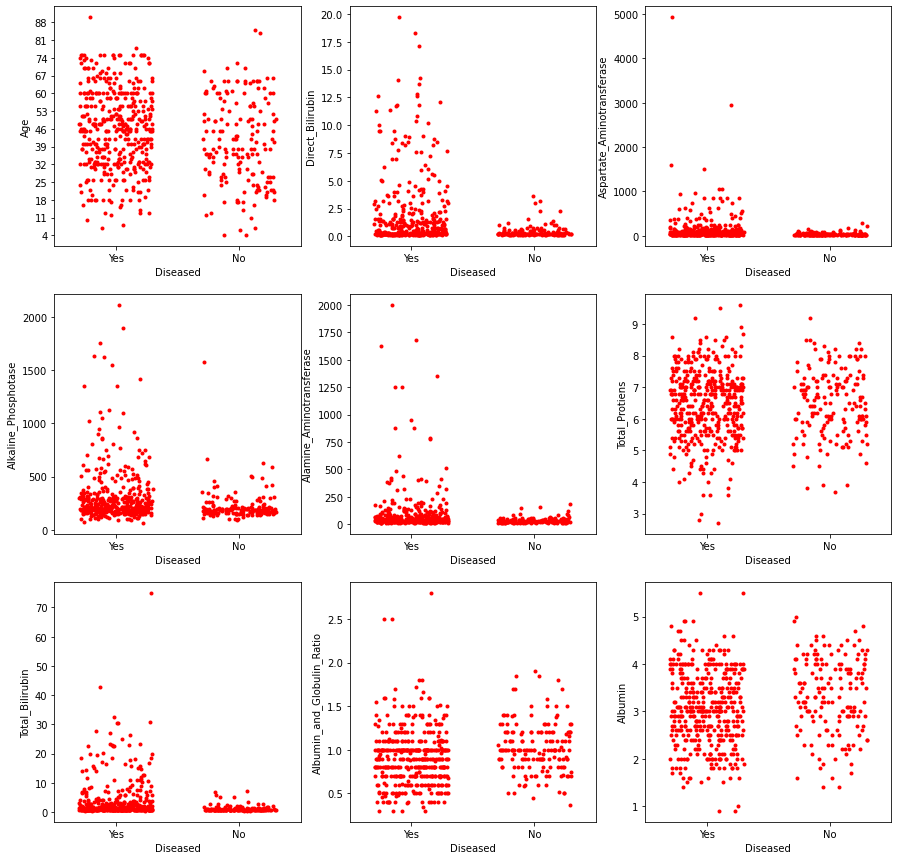
\includegraphics{output_214_0.png}
\caption{Diagrama de puntos Diseased en función de los predictores
cuantitativos}
\end{figure}

\newpage

\hypertarget{arboles-de-clasificaciuxf3n-en-r}{%
\subsection{\texorpdfstring{Arboles de clasificación en \texttt{R}
}{Arboles de clasificación en R }}\label{arboles-de-clasificaciuxf3n-en-r}}

\hypertarget{algoritmo-rpart-con-r}{%
\subsubsection{\texorpdfstring{Algoritmo \texttt{rpart} con \texttt{R}
}{Algoritmo rpart con R }}\label{algoritmo-rpart-con-r}}

\begin{Shaded}
\begin{Highlighting}[]
\SpecialCharTok{\%\%}\NormalTok{R}

\FunctionTok{library}\NormalTok{(rpart)}
\FunctionTok{library}\NormalTok{(rpart.plot)}
\FunctionTok{library}\NormalTok{(caret)}
\FunctionTok{library}\NormalTok{(tidyverse)}
\end{Highlighting}
\end{Shaded}

Vamos a hacer la visualización del arbol con \texttt{rpart}

\begin{Shaded}
\begin{Highlighting}[]
\SpecialCharTok{\%\%}\NormalTok{R}

\FunctionTok{set.seed}\NormalTok{(}\DecValTok{0}\NormalTok{)}
\NormalTok{datos\_entreno}\OtherTok{\textless{}{-}}\FunctionTok{sample\_frac}\NormalTok{(ilpd,}\FloatTok{0.75}\NormalTok{) }\CommentTok{\# fraccionamos la muestra en entrenamiento y test}
\NormalTok{datos\_test}\OtherTok{\textless{}{-}}\FunctionTok{setdiff}\NormalTok{(ilpd,datos\_entreno)}

\NormalTok{arbol\_0}\OtherTok{\textless{}{-}}\FunctionTok{rpart}\NormalTok{(diseased}\SpecialCharTok{\textasciitilde{}}\NormalTok{.,}\AttributeTok{data =}\NormalTok{ datos\_entreno, }\AttributeTok{method =} \StringTok{"class"}\NormalTok{, }\AttributeTok{cp=}\FloatTok{0.01}\NormalTok{)}
\FunctionTok{rpart.plot}\NormalTok{(arbol\_0, }
           \AttributeTok{extra =} \DecValTok{104}\NormalTok{,          }\CommentTok{\# show fitted class, probs, percentages}
           \AttributeTok{box.palette =} \StringTok{"GnBu"}\NormalTok{, }\CommentTok{\# color scheme}
           \AttributeTok{branch.lty =} \DecValTok{3}\NormalTok{,       }\CommentTok{\# dotted branch lines}
           \AttributeTok{shadow.col =} \StringTok{"gray"}\NormalTok{,  }\CommentTok{\# shadows under the node boxes}
           \AttributeTok{nn =} \ConstantTok{TRUE}\NormalTok{)}
\end{Highlighting}
\end{Shaded}

\begin{figure}
\centering
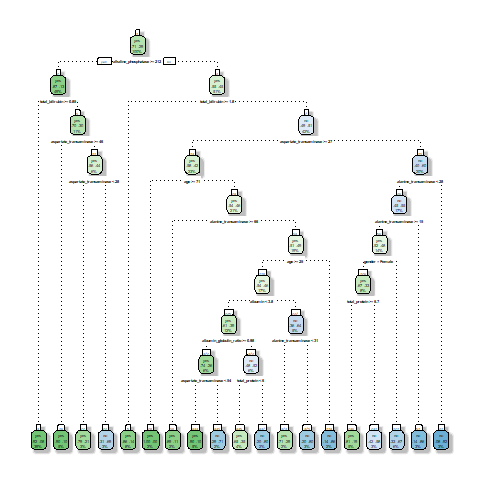
\includegraphics{output_222_0.png}
\caption{Arbol rpart con R}
\end{figure}

\newpage

Ahora vamos a calcular las predicciones y la matriz de confusión:

\begin{Shaded}
\begin{Highlighting}[]
\SpecialCharTok{\%\%}\NormalTok{R}

\NormalTok{prediccion1}\OtherTok{\textless{}{-}}\FunctionTok{predict}\NormalTok{(arbol\_0,}\AttributeTok{newdata=}\NormalTok{datos\_test,}\AttributeTok{type=}\StringTok{"class"}\NormalTok{)}

\NormalTok{matriz\_confusion1}\OtherTok{\textless{}{-}}\FunctionTok{confusionMatrix}\NormalTok{(prediccion1,datos\_test[[}\StringTok{"diseased"}\NormalTok{]])}
\end{Highlighting}
\end{Shaded}

\begin{Shaded}
\begin{Highlighting}[]
\SpecialCharTok{\%\%}\NormalTok{R}

\NormalTok{prediccion1}
\end{Highlighting}
\end{Shaded}

\begin{verbatim}
  1   2   3   4   5   6   7   8   9  10  11  12  13  14  15  16  17  18  19  20 
 no  no yes yes yes yes  no yes  no yes yes yes yes  no  no yes yes yes yes yes 
 21  22  23  24  25  26  27  28  29  30  31  32  33  34  35  36  37  38  39  40 
yes yes yes yes  no yes yes yes yes yes yes yes yes yes yes yes yes yes yes yes 
 41  42  43  44  45  46  47  48  49  50  51  52  53  54  55  56  57  58  59  60 
 no yes  no  no yes yes yes  no yes yes yes  no yes yes yes  no yes yes yes yes 
 61  62  63  64  65  66  67  68  69  70  71  72  73  74  75  76  77  78  79  80 
yes yes yes  no  no yes yes  no yes yes yes  no yes yes  no  no yes yes yes yes 
 81  82  83  84  85  86  87  88  89  90  91  92  93  94  95  96  97  98  99 100 
yes yes  no yes  no yes yes yes yes yes  no yes  no  no  no yes yes  no yes yes 
101 102 103 104 105 106 107 108 109 110 111 112 113 114 115 116 117 118 119 120 
yes yes yes yes yes  no  no yes yes yes  no  no  no yes  no yes yes yes  no yes 
121 122 123 124 125 126 127 128 129 130 131 132 133 134 135 136 137 138 139 140 
yes yes yes yes  no yes yes yes  no yes yes  no yes yes yes yes yes yes yes yes 
141 
yes 
Levels: yes no
\end{verbatim}

\begin{Shaded}
\begin{Highlighting}[]
\SpecialCharTok{\%\%}\NormalTok{R}

\NormalTok{matriz\_confusion1}
\end{Highlighting}
\end{Shaded}

\begin{verbatim}
Confusion Matrix and Statistics

          Reference
Prediction yes no
       yes  80 25
       no   22 14
                                          
               Accuracy : 0.6667          
                 95% CI : (0.5824, 0.7437)
    No Information Rate : 0.7234          
    P-Value [Acc > NIR] : 0.9431          
                                          
                  Kappa : 0.1468          
                                          
 Mcnemar's Test P-Value : 0.7705          
                                          
            Sensitivity : 0.7843          
            Specificity : 0.3590          
         Pos Pred Value : 0.7619          
         Neg Pred Value : 0.3889          
             Prevalence : 0.7234          
         Detection Rate : 0.5674          
   Detection Prevalence : 0.7447          
      Balanced Accuracy : 0.5716          
                                          
       'Positive' Class : yes             
                                          
\end{verbatim}

\vspace{0.25cm}

Debido a la alta complejidad de estos arboles le vamos a hacer un
proceso de prepoda, para ello podemos hacer uso tanto del parámetro cp o
directamente manipulando los hiperparametros de los modelos.

\vspace{0.25cm}

Arbol podado con una profundidad maxima de 4:

\begin{Shaded}
\begin{Highlighting}[]
\SpecialCharTok{\%\%}\NormalTok{R}

\FunctionTok{set.seed}\NormalTok{(}\DecValTok{0}\NormalTok{)}
\NormalTok{datos\_entreno2}\OtherTok{\textless{}{-}}\FunctionTok{sample\_frac}\NormalTok{(ilpd,}\FloatTok{0.75}\NormalTok{)  }\CommentTok{\# Separamos los datos de entrenamiento}
\NormalTok{datos\_test2}\OtherTok{\textless{}{-}}\FunctionTok{setdiff}\NormalTok{(ilpd, datos\_entreno2) }\CommentTok{\# Separamos los datos de test}

\NormalTok{arbol\_1}\OtherTok{\textless{}{-}}\FunctionTok{rpart}\NormalTok{(diseased}\SpecialCharTok{\textasciitilde{}}\NormalTok{.,}\AttributeTok{data=}\NormalTok{datos\_entreno2, }\AttributeTok{maxdepth=}\DecValTok{4}\NormalTok{, }\AttributeTok{method =} \StringTok{"class"}\NormalTok{) }\CommentTok{\# Cambiamos la profundidad}
\FunctionTok{rpart.plot}\NormalTok{(arbol\_1, }
           \AttributeTok{extra =} \DecValTok{104}\NormalTok{,          }\CommentTok{\# show fitted class, probs, percentages}
           \AttributeTok{box.palette =} \StringTok{"GnBu"}\NormalTok{, }\CommentTok{\# color scheme}
           \AttributeTok{branch.lty =} \DecValTok{3}\NormalTok{,       }\CommentTok{\# dotted branch lines}
           \AttributeTok{shadow.col =} \StringTok{"gray"}\NormalTok{,  }\CommentTok{\# shadows under the node boxes}
           \AttributeTok{nn =} \ConstantTok{TRUE}\NormalTok{)}
\end{Highlighting}
\end{Shaded}

\begin{figure}
\centering
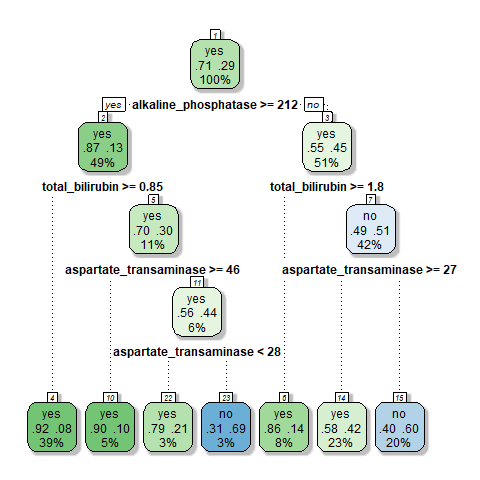
\includegraphics{output_234_0.png}
\caption{Arbol rpart podado en R}
\end{figure}

\newpage

Con esto hemos conseguido un modelo mucho más simple que el anterior sin
prepoda. El cual es más facil de interpretar.

En estos gráficos, cada uno de los rectángulos representa un nodo de
nuestro árbol, con su regla de clasificación.

Cada nodo está coloreado de acuerdo a la categoría mayoritaria entre los
datos que agrupa. Esta es la categoría que ha predicho el modelo para
ese grupo.

Dentro del rectángulo de cada nodo se nos muestra qué proporción de
casos pertenecen a cada categoría y la proporción del total de datos que
han sido agrupados allí.

Estas proporciones nos dan una idea de la precisión de nuestro modelo al
hacer predicciones.

\vspace{0.25cm}

Calculamos las predicciones y la matriz de confusión:

\begin{Shaded}
\begin{Highlighting}[]
\SpecialCharTok{\%\%}\NormalTok{R}

\NormalTok{prediccion2 }\OtherTok{\textless{}{-}}\FunctionTok{predict}\NormalTok{(arbol\_1,}\AttributeTok{newdata=}\NormalTok{datos\_test2,}\AttributeTok{type=}\StringTok{"class"}\NormalTok{)}
\NormalTok{matriz\_confusion2}\OtherTok{\textless{}{-}}\FunctionTok{confusionMatrix}\NormalTok{(prediccion2,datos\_test2[[}\StringTok{"diseased"}\NormalTok{]])}
\end{Highlighting}
\end{Shaded}

\begin{Shaded}
\begin{Highlighting}[]
\SpecialCharTok{\%\%}\NormalTok{R}

\NormalTok{prediccion2}
\end{Highlighting}
\end{Shaded}

\begin{verbatim}
  1   2   3   4   5   6   7   8   9  10  11  12  13  14  15  16  17  18  19  20 
 no  no yes yes yes yes  no yes  no yes yes yes yes  no  no yes yes yes yes yes 
 21  22  23  24  25  26  27  28  29  30  31  32  33  34  35  36  37  38  39  40 
yes yes yes yes  no yes yes yes yes yes yes yes yes yes yes yes yes yes yes yes 
 41  42  43  44  45  46  47  48  49  50  51  52  53  54  55  56  57  58  59  60 
 no yes yes  no yes yes yes  no yes yes yes yes yes  no yes yes yes yes yes yes 
 61  62  63  64  65  66  67  68  69  70  71  72  73  74  75  76  77  78  79  80 
yes yes yes  no  no yes yes  no yes yes yes yes yes yes yes yes yes yes yes yes 
 81  82  83  84  85  86  87  88  89  90  91  92  93  94  95  96  97  98  99 100 
yes yes  no yes yes yes yes yes yes yes yes yes  no yes  no yes yes  no yes yes 
101 102 103 104 105 106 107 108 109 110 111 112 113 114 115 116 117 118 119 120 
yes yes yes yes yes yes  no yes yes yes  no  no  no yes  no yes yes yes yes yes 
121 122 123 124 125 126 127 128 129 130 131 132 133 134 135 136 137 138 139 140 
yes yes yes yes yes yes yes yes  no yes yes  no yes yes yes yes yes yes yes yes 
141 
yes 
Levels: yes no
\end{verbatim}

\newpage

\begin{Shaded}
\begin{Highlighting}[]
\SpecialCharTok{\%\%}\NormalTok{R}

\NormalTok{matriz\_confusion2}
\end{Highlighting}
\end{Shaded}

\begin{verbatim}
Confusion Matrix and Statistics

          Reference
Prediction yes no
       yes  87 29
       no   15 10
                                          
               Accuracy : 0.6879          
                 95% CI : (0.6045, 0.7633)
    No Information Rate : 0.7234          
    P-Value [Acc > NIR] : 0.84963         
                                          
                  Kappa : 0.123           
                                          
 Mcnemar's Test P-Value : 0.05002         
                                          
            Sensitivity : 0.8529          
            Specificity : 0.2564          
         Pos Pred Value : 0.7500          
         Neg Pred Value : 0.4000          
             Prevalence : 0.7234          
         Detection Rate : 0.6170          
   Detection Prevalence : 0.8227          
      Balanced Accuracy : 0.5547          
                                          
       'Positive' Class : yes             
                                          
\end{verbatim}

Se puede ver como hemos mejorado un poco la precisión de la predicción
simplemente cambiando la profundidad máxima. Cabe remarcar que el
algoritmo de los CART utilizan el índice de Gini como criterio de
división.

\newpage

\hypertarget{algoritmo-c5.0-con-r}{%
\subsubsection{\texorpdfstring{Algoritmo C5.0 con \texttt{R}
}{Algoritmo C5.0 con R }}\label{algoritmo-c5.0-con-r}}

Cargamos el paquete específico del Arbol de clasificación C5.0

\begin{Shaded}
\begin{Highlighting}[]
\SpecialCharTok{\%\%}\NormalTok{R}

\CommentTok{\# install.packages("C50",dependencies=TRUE)}

\FunctionTok{library}\NormalTok{(C50)}
\end{Highlighting}
\end{Shaded}

Realizamos la partición en datos de entrenaminento y test:

\begin{Shaded}
\begin{Highlighting}[]
\SpecialCharTok{\%\%}\NormalTok{R}

\FunctionTok{set.seed}\NormalTok{(}\DecValTok{0}\NormalTok{)}
\NormalTok{tamano\_total}\OtherTok{\textless{}{-}}\FunctionTok{nrow}\NormalTok{(ilpd)}
\NormalTok{tamano\_entreno}\OtherTok{\textless{}{-}}\FunctionTok{round}\NormalTok{(tamano\_total}\SpecialCharTok{*}\FloatTok{0.75}\NormalTok{)}
\NormalTok{datos\_indices}\OtherTok{\textless{}{-}}\FunctionTok{sample}\NormalTok{(}\DecValTok{1}\SpecialCharTok{:}\NormalTok{tamano\_total,}\AttributeTok{size =}\NormalTok{ tamano\_entreno)}
\NormalTok{datos\_entreno}\OtherTok{\textless{}{-}}\NormalTok{ilpd[datos\_indices,]}
\NormalTok{datos\_test}\OtherTok{\textless{}{-}}\NormalTok{ilpd[}\SpecialCharTok{{-}}\NormalTok{datos\_indices,]}
\end{Highlighting}
\end{Shaded}

Las siguientes proporciones deberían de ser relativamente similares para
que los arboles den unos buenos resultados:

\begin{Shaded}
\begin{Highlighting}[]
\SpecialCharTok{\%\%}\NormalTok{R}

\FunctionTok{round}\NormalTok{(}\FunctionTok{table}\NormalTok{(datos\_entreno}\SpecialCharTok{$}\NormalTok{diseased)}\SpecialCharTok{/}\FunctionTok{nrow}\NormalTok{(datos\_entreno), }\DecValTok{3}\NormalTok{)}
\end{Highlighting}
\end{Shaded}

\begin{verbatim}
  yes    no 
0.709 0.291 
\end{verbatim}

\begin{Shaded}
\begin{Highlighting}[]
\SpecialCharTok{\%\%}\NormalTok{R}

\FunctionTok{round}\NormalTok{(}\FunctionTok{table}\NormalTok{(datos\_test}\SpecialCharTok{$}\NormalTok{diseased)}\SpecialCharTok{/}\FunctionTok{nrow}\NormalTok{(datos\_test), }\DecValTok{3}\NormalTok{)}
\end{Highlighting}
\end{Shaded}

\begin{verbatim}
  yes    no 
0.726 0.274 
\end{verbatim}

Ejecución del modelo de clasificación C5.0

\begin{Shaded}
\begin{Highlighting}[]
\SpecialCharTok{\%\%}\NormalTok{R}

\NormalTok{modeloC50 }\OtherTok{\textless{}{-}} \FunctionTok{C5.0}\NormalTok{(diseased}\SpecialCharTok{\textasciitilde{}}\NormalTok{.,}\AttributeTok{data=}\NormalTok{datos\_entreno,}\AttributeTok{trials=}\DecValTok{1}\NormalTok{,}\AttributeTok{rules=}\ConstantTok{FALSE}\NormalTok{)}
\end{Highlighting}
\end{Shaded}

\newpage

Información del modelo creado

\begin{Shaded}
\begin{Highlighting}[]
\SpecialCharTok{\%\%}\NormalTok{R}

\FunctionTok{summary}\NormalTok{(modeloC50)}
\end{Highlighting}
\end{Shaded}

\begin{verbatim}
Call:
C5.0.formula(formula = diseased ~ ., data = datos_entreno, trials = 1, rules
 = FALSE)


C5.0 [Release 2.07 GPL Edition]     Thu Oct 13 16:14:45 2022
-------------------------------

Class specified by attribute `outcome'

Read 437 cases (11 attributes) from undefined.data

Decision tree:

direct_bilirubin > 0.9: yes (135/9)
direct_bilirubin <= 0.9:
:...alanine_transaminase > 65:
    :...albumin <= 3.9: yes (35/1)
    :   albumin > 3.9:
    :   :...aspartate_transaminase <= 99: no (4/1)
    :       aspartate_transaminase > 99: yes (4)
    alanine_transaminase <= 65:
    :...alkaline_phosphatase > 211:
        :...total_bilirubin <= 0.8:
        :   :...gender = Female:
        :   :   :...age <= 39: yes (2)
        :   :   :   age > 39: no (5)
        :   :   gender = Male:
        :   :   :...age <= 13: no (3)
        :   :       age > 13:
        :   :       :...albumin_globulin_ratio <= 0.55: no (2)
        :   :           albumin_globulin_ratio > 0.55: yes (25/4)
        :   total_bilirubin > 0.8:
        :   :...age > 37: yes (27/1)
        :       age <= 37:
        :       :...total_bilirubin > 1.6: no (2)
        :           total_bilirubin <= 1.6:
        :           :...alanine_transaminase <= 23: no (2)
        :               alanine_transaminase > 23: yes (10/1)
        alkaline_phosphatase <= 211:
        :...direct_bilirubin <= 0.1:
            :...gender = Male: yes (21/5)
            :   gender = Female:
            :   :...alkaline_phosphatase <= 168: no (4)
            :       alkaline_phosphatase > 168: yes (8/2)
            direct_bilirubin > 0.1:
            :...total_bilirubin <= 0.7:
                :...alanine_transaminase > 33:
                :   :...aspartate_transaminase > 64: yes (3)
                :   :   aspartate_transaminase <= 64:
                :   :   :...aspartate_transaminase <= 41: yes (2)
                :   :       aspartate_transaminase > 41: no (2)
                :   alanine_transaminase <= 33:
                :   :...albumin_globulin_ratio > 0.9: no (19)
                :       albumin_globulin_ratio <= 0.9:
                :       :...gender = Female:
                :           :...alkaline_phosphatase <= 176: yes (3/1)
                :           :   alkaline_phosphatase > 176: no (3)
                :           gender = Male:
                :           :...age <= 34: no (2)
                :               age > 34: yes (5/1)
                total_bilirubin > 0.7:
                :...gender = Female:
                    :...alanine_transaminase > 29: no (7)
                    :   alanine_transaminase <= 29:
                    :   :...total_bilirubin > 0.9: no (7/1)
                    :       total_bilirubin <= 0.9:
                    :       :...albumin <= 4.3: yes (23/3)
                    :           albumin > 4.3: no (4/1)
                    gender = Male:
                    :...aspartate_transaminase <= 25:
                        :...albumin <= 3.9: no (18/1)
                        :   albumin > 3.9: yes (5/1)
                        aspartate_transaminase > 25:
                        :...aspartate_transaminase > 70: no (4)
                            aspartate_transaminase <= 70:
                            :...albumin_globulin_ratio <= 0.58: no (3)
                                albumin_globulin_ratio > 0.58: yes (38/11)


Evaluation on training data (437 cases):

        Decision Tree   
      ----------------  
      Size      Errors  

        33   44(10.1%)   <<


       (a)   (b)    <-classified as
      ----  ----
       306     4    (a): class yes
        40    87    (b): class no


    Attribute usage:

    100.00% direct_bilirubin
     69.11% alanine_transaminase
     59.27% alkaline_phosphatase
     51.72% total_bilirubin
     43.94% gender
     22.88% albumin_globulin_ratio
     21.28% albumin
     19.45% age
     18.99% aspartate_transaminase


Time: 0.0 secs
\end{verbatim}

Podemos ver el gráfico del modelo:

\begin{Shaded}
\begin{Highlighting}[]
\SpecialCharTok{\%\%}\NormalTok{R}

\FunctionTok{plot}\NormalTok{(modeloC50)}
\end{Highlighting}
\end{Shaded}

\begin{figure}
\centering
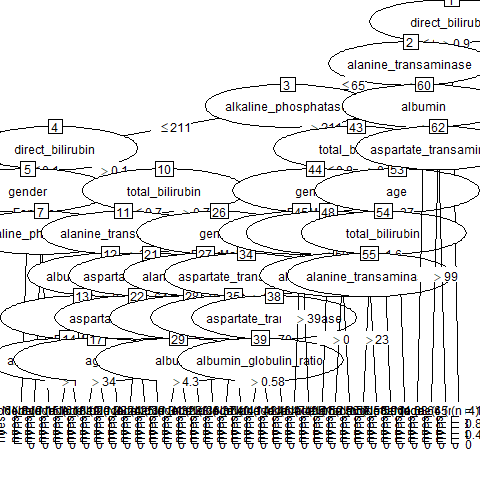
\includegraphics[width=4.6875in,height=3.64583in]{output_265_0.png}
\caption{Arbol C5.0 en R}
\end{figure}

\newpage

Calculamos las predicciones del modelo:

\begin{Shaded}
\begin{Highlighting}[]
\SpecialCharTok{\%\%}\NormalTok{R}

\NormalTok{(prediccion}\OtherTok{\textless{}{-}}\FunctionTok{predict}\NormalTok{(modeloC50, }\AttributeTok{newdata =}\NormalTok{ datos\_test,}\AttributeTok{type=}\StringTok{"class"}\NormalTok{))}
\end{Highlighting}
\end{Shaded}

\begin{verbatim}
  [1] no  yes yes yes yes yes no  yes yes yes yes no  yes no  yes yes yes no 
 [19] yes yes yes yes yes yes yes yes yes yes no  yes yes yes yes yes yes yes
 [37] yes yes yes yes yes yes yes yes yes no  yes no  no  yes yes yes no  yes
 [55] yes yes yes yes yes yes yes yes yes yes yes yes yes yes yes yes yes yes
 [73] yes yes yes yes no  yes no  no  yes yes yes yes yes yes yes yes yes yes
 [91] yes yes yes yes yes yes yes no  yes no  yes yes no  yes yes yes yes yes
[109] yes yes yes yes yes no  yes no  yes no  yes no  yes yes no  yes yes yes
[127] yes yes yes no  yes yes yes no  yes yes no  yes yes yes yes yes yes yes
[145] yes yes
Levels: yes no
\end{verbatim}

\vspace{0.2cm}

Calculamos la matriz de confusión:

\begin{Shaded}
\begin{Highlighting}[]
\SpecialCharTok{\%\%}\NormalTok{R}

\NormalTok{(matriz\_confusion}\OtherTok{\textless{}{-}}\FunctionTok{table}\NormalTok{(}\AttributeTok{predicho=}\NormalTok{prediccion, }\AttributeTok{real=}\NormalTok{datos\_test}\SpecialCharTok{$}\NormalTok{diseased))}
\end{Highlighting}
\end{Shaded}

\begin{verbatim}
        real
predicho yes no
     yes  92 30
     no   14 10
\end{verbatim}

\vspace{0.2cm}

Calculamos la tasa de acierto en la clasificacion (TAC) obtenida parte
del modelo, es decir el porcentaje de clasificaciones correctas.

\begin{Shaded}
\begin{Highlighting}[]
\SpecialCharTok{\%\%}\NormalTok{R}

\DecValTok{100}\SpecialCharTok{*}\FunctionTok{sum}\NormalTok{(}\FunctionTok{diag}\NormalTok{(matriz\_confusion))}\SpecialCharTok{/}\FunctionTok{sum}\NormalTok{(matriz\_confusion)}
\end{Highlighting}
\end{Shaded}

\begin{verbatim}
[1] 69.86301
\end{verbatim}

TAC = 0.6986

\vspace{0.2cm}

Calculamos la tasa de error de clasificacion (TEC = 1 - TAC) cometido
por el modelo, que es el porcentaje de clasificaciones incorrectas

\begin{Shaded}
\begin{Highlighting}[]
\SpecialCharTok{\%\%}\NormalTok{R}

\NormalTok{error\_clas}\OtherTok{\textless{}{-}}\FunctionTok{round}\NormalTok{(}\FunctionTok{mean}\NormalTok{(prediccion }\SpecialCharTok{!=}\NormalTok{ datos\_test}\SpecialCharTok{$}\NormalTok{diseased),}\DecValTok{3}\NormalTok{)}
\FunctionTok{paste}\NormalTok{(}
  \StringTok{"El error de clasificacion es del:"}\NormalTok{,}\DecValTok{100}\SpecialCharTok{*}\NormalTok{error\_clas,}\StringTok{"\%."}\NormalTok{,}\FunctionTok{sum}\NormalTok{(prediccion}\SpecialCharTok{==}\NormalTok{datos\_test}\SpecialCharTok{$}\NormalTok{diseased),}\StringTok{"clasificaciones correctas de un total de"}\NormalTok{,}\FunctionTok{length}\NormalTok{(prediccion)}
\NormalTok{)}
\end{Highlighting}
\end{Shaded}

\begin{verbatim}
[1] "El error de clasificacion es del: 30.1 %. 102 clasificaciones correctas de un total de 146"
\end{verbatim}

TEC = 0.301

\vspace{1cm}

Ahora vamos a podar el arbol con la libreria C5.0

Seleccionamos la submuestra del 75\% de los datos

\begin{Shaded}
\begin{Highlighting}[]
\SpecialCharTok{\%\%}\NormalTok{R}

\FunctionTok{set.seed}\NormalTok{(}\DecValTok{0}\NormalTok{)}
\NormalTok{tamano\_total}\OtherTok{\textless{}{-}}\FunctionTok{nrow}\NormalTok{(ilpd)}
\NormalTok{tamano\_entreno}\OtherTok{\textless{}{-}}\FunctionTok{round}\NormalTok{(tamano\_total}\SpecialCharTok{*}\FloatTok{0.75}\NormalTok{)}
\NormalTok{datos\_indices}\OtherTok{\textless{}{-}}\FunctionTok{sample}\NormalTok{(}\DecValTok{1}\SpecialCharTok{:}\NormalTok{tamano\_total,}\AttributeTok{size =}\NormalTok{ tamano\_entreno)}
\NormalTok{datos\_entreno}\OtherTok{\textless{}{-}}\NormalTok{ilpd[datos\_indices,]}
\NormalTok{datos\_test}\OtherTok{\textless{}{-}}\NormalTok{ilpd[}\SpecialCharTok{{-}}\NormalTok{datos\_indices,]}
\end{Highlighting}
\end{Shaded}

Las siguientes proporciones deberían de ser relativamente similares para
que los arboles den unos buenos resultados:

\begin{Shaded}
\begin{Highlighting}[]
\SpecialCharTok{\%\%}\NormalTok{R}

\FunctionTok{round}\NormalTok{(}\FunctionTok{table}\NormalTok{(datos\_entreno}\SpecialCharTok{$}\NormalTok{diseased)}\SpecialCharTok{/}\FunctionTok{nrow}\NormalTok{(datos\_entreno), }\DecValTok{3}\NormalTok{)}
\end{Highlighting}
\end{Shaded}

\begin{verbatim}
  yes    no 
0.709 0.291 
\end{verbatim}

\begin{Shaded}
\begin{Highlighting}[]
\SpecialCharTok{\%\%}\NormalTok{R}

\FunctionTok{round}\NormalTok{(}\FunctionTok{table}\NormalTok{(datos\_test}\SpecialCharTok{$}\NormalTok{diseased)}\SpecialCharTok{/}\FunctionTok{nrow}\NormalTok{(datos\_test), }\DecValTok{3}\NormalTok{)}
\end{Highlighting}
\end{Shaded}

\begin{verbatim}
  yes    no 
0.726 0.274 
\end{verbatim}

Ejecución del arbol de clasificación podado con la libreria C5.0

\begin{Shaded}
\begin{Highlighting}[]
\SpecialCharTok{\%\%}\NormalTok{R}


\NormalTok{modeloC50}\OtherTok{\textless{}{-}}\FunctionTok{C5.0}\NormalTok{(diseased}\SpecialCharTok{\textasciitilde{}}\NormalTok{.,}\AttributeTok{data=}\NormalTok{datos\_entreno,}\AttributeTok{trials=}\DecValTok{1}\NormalTok{,}\AttributeTok{rules=}\ConstantTok{FALSE}\NormalTok{,}\AttributeTok{control =} \FunctionTok{C5.0Control}\NormalTok{(}\AttributeTok{minCases =} \DecValTok{10}\NormalTok{,}\AttributeTok{earlyStopping =} \ConstantTok{TRUE}\NormalTok{))}
\end{Highlighting}
\end{Shaded}

Información del modelo creado

\begin{Shaded}
\begin{Highlighting}[]
\SpecialCharTok{\%\%}\NormalTok{R}

\FunctionTok{summary}\NormalTok{(modeloC50)}
\end{Highlighting}
\end{Shaded}

\begin{verbatim}
Call:
C5.0.formula(formula = diseased ~ ., data = datos_entreno, trials = 1, rules
 = FALSE, control = C5.0Control(minCases = 10, earlyStopping = TRUE))


C5.0 [Release 2.07 GPL Edition]     Thu Oct 13 16:14:56 2022
-------------------------------

Class specified by attribute `outcome'

Read 437 cases (11 attributes) from undefined.data

Decision tree:

direct_bilirubin > 0.9: yes (135/9)
direct_bilirubin <= 0.9:
:...alanine_transaminase > 65: yes (43/4)
    alanine_transaminase <= 65:
    :...alkaline_phosphatase > 211: yes (78/20)
        alkaline_phosphatase <= 211:
        :...direct_bilirubin <= 0.1: yes (33/11)
            direct_bilirubin > 0.1:
            :...total_bilirubin <= 0.7: no (39/11)
                total_bilirubin > 0.7:
                :...gender = Female:
                    :...total_bilirubin <= 0.8: yes (20/5)
                    :   total_bilirubin > 0.8: no (21/7)
                    gender = Male:
                    :...aspartate_transaminase <= 25: no (23/5)
                        aspartate_transaminase > 25: yes (45/18)


Evaluation on training data (437 cases):

        Decision Tree   
      ----------------  
      Size      Errors  

         9   90(20.6%)   <<


       (a)   (b)    <-classified as
      ----  ----
       287    23    (a): class yes
        67    60    (b): class no


    Attribute usage:

    100.00% direct_bilirubin
     69.11% alanine_transaminase
     59.27% alkaline_phosphatase
     33.87% total_bilirubin
     24.94% gender
     15.56% aspartate_transaminase


Time: 0.0 secs
\end{verbatim}

Gráfico del modelo:

\begin{Shaded}
\begin{Highlighting}[]
\SpecialCharTok{\%\%}\NormalTok{R}

\FunctionTok{plot}\NormalTok{(modeloC50)}
\end{Highlighting}
\end{Shaded}

\begin{figure}
\centering
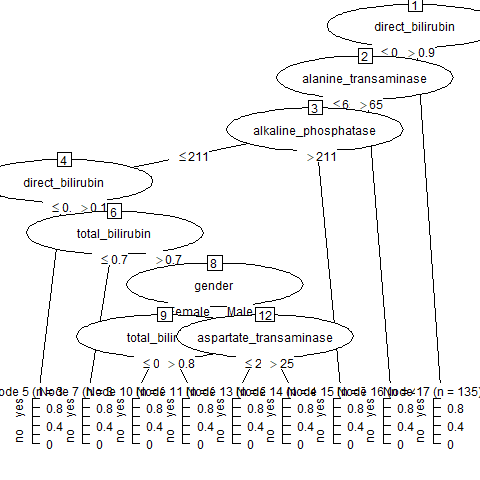
\includegraphics[width=4.375in,height=3.125in]{output_295_0.png}
\caption{Arbol C5.0 podado con R}
\end{figure}

\newpage

Calculamos las predicciones:

\begin{Shaded}
\begin{Highlighting}[]
\SpecialCharTok{\%\%}\NormalTok{R}

\NormalTok{(prediccion}\OtherTok{\textless{}{-}}\FunctionTok{predict}\NormalTok{(modeloC50, }\AttributeTok{newdata =}\NormalTok{ datos\_test,}\AttributeTok{type=}\StringTok{"class"}\NormalTok{))}
\end{Highlighting}
\end{Shaded}

\begin{verbatim}
  [1] no  no  yes yes yes yes yes yes yes no  yes yes yes yes yes yes yes yes
 [19] yes yes yes yes yes yes yes yes yes yes no  yes yes yes yes yes yes yes
 [37] yes yes yes yes yes yes yes yes yes no  yes no  no  yes yes yes yes yes
 [55] yes yes yes yes yes yes yes yes yes no  no  yes no  yes no  no  yes yes
 [73] no  yes yes yes yes yes no  yes yes yes yes yes yes yes yes no  yes no 
 [91] yes no  yes yes yes yes yes no  yes no  yes yes no  yes no  yes yes yes
[109] yes yes yes yes yes yes yes no  yes yes no  no  yes yes yes yes yes yes
[127] yes yes yes yes yes yes yes no  yes yes no  yes yes yes yes yes yes yes
[145] yes yes
Levels: yes no
\end{verbatim}

Calculamos la matriz de confusión:

\begin{Shaded}
\begin{Highlighting}[]
\SpecialCharTok{\%\%}\NormalTok{R}

\NormalTok{(matriz\_confusion}\OtherTok{\textless{}{-}}\FunctionTok{table}\NormalTok{(}\AttributeTok{predicho=}\NormalTok{prediccion, }\AttributeTok{real=}\NormalTok{datos\_test}\SpecialCharTok{$}\NormalTok{diseased))}
\end{Highlighting}
\end{Shaded}

\begin{verbatim}
        real
predicho yes no
     yes  92 28
     no   14 12
\end{verbatim}

\vspace{0.5cm}

Porcentaje de clasificados correctamente:

\begin{Shaded}
\begin{Highlighting}[]
\SpecialCharTok{\%\%}\NormalTok{R}

\DecValTok{100}\SpecialCharTok{*}\FunctionTok{sum}\NormalTok{(}\FunctionTok{diag}\NormalTok{(matriz\_confusion))}\SpecialCharTok{/}\FunctionTok{sum}\NormalTok{(matriz\_confusion)}
\end{Highlighting}
\end{Shaded}

\begin{verbatim}
[1] 71.23288
\end{verbatim}

TAC = 0.7123

\newpage

Error de clasificación :

\begin{Shaded}
\begin{Highlighting}[]
\SpecialCharTok{\%\%}\NormalTok{R}

\NormalTok{error\_clas}\OtherTok{\textless{}{-}}\FunctionTok{round}\NormalTok{(}\FunctionTok{mean}\NormalTok{(prediccion }\SpecialCharTok{!=}\NormalTok{ datos\_test}\SpecialCharTok{$}\NormalTok{diseased),}\DecValTok{3}\NormalTok{)}
\FunctionTok{paste}\NormalTok{(}
  \StringTok{"El error de clasificacion es del:"}\NormalTok{,}\DecValTok{100}\SpecialCharTok{*}\NormalTok{error\_clas,}\StringTok{"\%."}\NormalTok{,}\FunctionTok{sum}\NormalTok{(prediccion}\SpecialCharTok{==}\NormalTok{datos\_test}\SpecialCharTok{$}\NormalTok{diseased),}\StringTok{"clasificaciones correctas de un total de"}\NormalTok{,}\FunctionTok{length}\NormalTok{(prediccion)}
\NormalTok{)}
\end{Highlighting}
\end{Shaded}

\begin{verbatim}
[1] "El error de clasificacion es del: 28.8 %. 104 clasificaciones correctas de un total de 146"
\end{verbatim}

TEC = 0.288

\vspace{1cm}

\hypertarget{algoritmo-cart-en-r-con-mlr3}{%
\subsubsection{\texorpdfstring{Algoritmo CART en \texttt{R} con
\texttt{mlr3}}{Algoritmo CART en R con mlr3}}\label{algoritmo-cart-en-r-con-mlr3}}

No es necesario preprocesar los datos para árboles (dummy y
normalización).

\begin{Shaded}
\begin{Highlighting}[]
\SpecialCharTok{\%\%}\NormalTok{R}

\CommentTok{\# install.packages(\textquotesingle{}mlr3extralearners\textquotesingle{})}

\FunctionTok{library}\NormalTok{(mlr3)}
\FunctionTok{library}\NormalTok{(mlr3learners)}
\end{Highlighting}
\end{Shaded}

\begin{verbatim}
R[write to console]: 
Attaching package: 'mlr3'


R[write to console]: The following object is masked from 'package:skimr':

    partition
\end{verbatim}

Creamos la tarea de clasificación:

\begin{Shaded}
\begin{Highlighting}[]
\SpecialCharTok{\%\%}\NormalTok{R}

\NormalTok{ILPD\_task }\OtherTok{\textless{}{-}} \FunctionTok{as\_task\_classif}\NormalTok{(ilpd , }\AttributeTok{target =} \StringTok{"diseased"}\NormalTok{)}
\end{Highlighting}
\end{Shaded}

\newpage

Partimos el data-set en parte de test y parte de train:

\begin{Shaded}
\begin{Highlighting}[]
\SpecialCharTok{\%\%}\NormalTok{R}

\NormalTok{res\_desc }\OtherTok{\textless{}{-}} \FunctionTok{rsmp}\NormalTok{(}\StringTok{"holdout"}\NormalTok{ , }\AttributeTok{ratio=}\FloatTok{0.75}\NormalTok{)}

\FunctionTok{set.seed}\NormalTok{(}\DecValTok{0}\NormalTok{)}

\NormalTok{res\_desc}\SpecialCharTok{$}\FunctionTok{instantiate}\NormalTok{(ILPD\_task)}
\end{Highlighting}
\end{Shaded}

Definimos el método de aprendizaje:

\begin{Shaded}
\begin{Highlighting}[]
\SpecialCharTok{\%\%}\NormalTok{R}

\NormalTok{tree\_learner }\OtherTok{\textless{}{-}} \FunctionTok{lrn}\NormalTok{(}\StringTok{"classif.rpart"}\NormalTok{ , }\AttributeTok{maxdepth=}\DecValTok{4}\NormalTok{)}
\end{Highlighting}
\end{Shaded}

Entrenamos y evaluamos el modelo:

\begin{Shaded}
\begin{Highlighting}[]
\SpecialCharTok{\%\%}\NormalTok{R}

\NormalTok{tree\_resample}\OtherTok{\textless{}{-}}\FunctionTok{resample}\NormalTok{(}\AttributeTok{task =}\NormalTok{ ILPD\_task, }\AttributeTok{learner =}\NormalTok{ tree\_learner,}\AttributeTok{resampling =}\NormalTok{ res\_desc,}\AttributeTok{store\_models =} \ConstantTok{TRUE}\NormalTok{)}
\end{Highlighting}
\end{Shaded}

\begin{verbatim}
INFO  [16:15:05.775] [mlr3] Applying learner 'classif.rpart' on task 'ilpd' (iter 1/1)
\end{verbatim}

Calculamos las predicciones:

\begin{Shaded}
\begin{Highlighting}[]
\SpecialCharTok{\%\%}\NormalTok{R}

\NormalTok{tree\_test}\OtherTok{\textless{}{-}}\NormalTok{tree\_resample}\SpecialCharTok{$}\FunctionTok{predictions}\NormalTok{()}
\NormalTok{tree\_test[[}\DecValTok{1}\NormalTok{]]}
\end{Highlighting}
\end{Shaded}

\begin{verbatim}
<PredictionClassif> for 146 observations:
    row_ids truth response
          4   yes       no
          9    no       no
         11   yes      yes
---                       
        575   yes      yes
        577   yes      yes
        583    no      yes
\end{verbatim}

\newpage

Calculamos la accuracy (que es la TAC):

\begin{Shaded}
\begin{Highlighting}[]
\SpecialCharTok{\%\%}\NormalTok{R}

\NormalTok{tree\_acc }\OtherTok{\textless{}{-}}\NormalTok{ tree\_resample}\SpecialCharTok{$}\FunctionTok{aggregate}\NormalTok{(}\FunctionTok{msr}\NormalTok{(}\StringTok{"classif.acc"}\NormalTok{))}

\NormalTok{tree\_acc}
\end{Highlighting}
\end{Shaded}

\begin{verbatim}
classif.acc 
  0.6917808 
\end{verbatim}

\vspace{0.25cm}

Visualizamos el modelo:

Primero obtenderemos la expresion en texto del modelo, luego su gráfico.

\begin{Shaded}
\begin{Highlighting}[]
\SpecialCharTok{\%\%}\NormalTok{R}

\NormalTok{tree\_learner}\OtherTok{\textless{}{-}}\NormalTok{tree\_resample}\SpecialCharTok{$}\NormalTok{learners[[}\DecValTok{1}\NormalTok{]]}
\NormalTok{tree\_learner}\SpecialCharTok{$}\NormalTok{model}
\end{Highlighting}
\end{Shaded}

\begin{verbatim}
n= 437 

node), split, n, loss, yval, (yprob)
      * denotes terminal node

 1) root 437 127 yes (0.70938215 0.29061785)  
   2) alkaline_phosphatase>=211.5 216  28 yes (0.87037037 0.12962963)  
     4) total_bilirubin>=0.85 169  14 yes (0.91715976 0.08284024) *
     5) total_bilirubin< 0.85 47  14 yes (0.70212766 0.29787234)  
      10) aspartate_transaminase>=45.5 20   2 yes (0.90000000 0.10000000) *
      11) aspartate_transaminase< 45.5 27  12 yes (0.55555556 0.44444444)  
        22) aspartate_transaminase< 27.5 14   3 yes (0.78571429 0.21428571) *
        23) aspartate_transaminase>=27.5 13   4 no (0.30769231 0.69230769) *
   3) alkaline_phosphatase< 211.5 221  99 yes (0.55203620 0.44796380)  
     6) total_bilirubin>=1.75 36   5 yes (0.86111111 0.13888889) *
     7) total_bilirubin< 1.75 185  91 no (0.49189189 0.50810811)  
      14) aspartate_transaminase>=26.5 99  42 yes (0.57575758 0.42424242) *
      15) aspartate_transaminase< 26.5 86  34 no (0.39534884 0.60465116) *
\end{verbatim}

\newpage

\begin{Shaded}
\begin{Highlighting}[]
\SpecialCharTok{\%\%}\NormalTok{R}

\FunctionTok{rpart.plot}\NormalTok{(tree\_learner}\SpecialCharTok{$}\NormalTok{model)}
\end{Highlighting}
\end{Shaded}

\begin{figure}
\centering
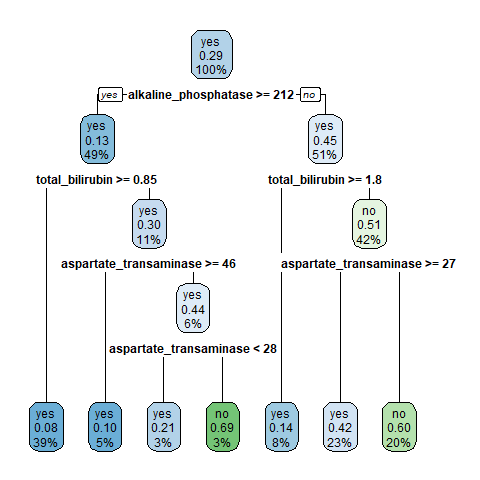
\includegraphics{output_342_0.png}
\caption{Arbol rpart podado con mlr3}
\end{figure}

\newpage

\hypertarget{algoritmo-c5.0-en-r-con-mlr3}{%
\subsubsection{\texorpdfstring{Algoritmo C5.0 en \texttt{R} con
\texttt{mlr3}
}{Algoritmo C5.0 en R con mlr3 }}\label{algoritmo-c5.0-en-r-con-mlr3}}

\begin{Shaded}
\begin{Highlighting}[]
\SpecialCharTok{\%\%}\NormalTok{R}

\FunctionTok{library}\NormalTok{(mlr3)}
\FunctionTok{library}\NormalTok{(mlr3learners)}
\FunctionTok{library}\NormalTok{(mlr3extralearners)}
\end{Highlighting}
\end{Shaded}

Cambiamos el tipo de los datos a numerico porque si no el algoritmo no
funciona.

\begin{Shaded}
\begin{Highlighting}[]
\SpecialCharTok{\%\%}\NormalTok{R}

\NormalTok{ilpd}\SpecialCharTok{$}\NormalTok{age}\OtherTok{\textless{}{-}}\FunctionTok{as.numeric}\NormalTok{(ilpd}\SpecialCharTok{$}\NormalTok{age)}
\NormalTok{ilpd}\SpecialCharTok{$}\NormalTok{alkaline\_phosphatase}\OtherTok{\textless{}{-}}\FunctionTok{as.numeric}\NormalTok{(ilpd}\SpecialCharTok{$}\NormalTok{alkaline\_phosphatase)}
\NormalTok{ilpd}\SpecialCharTok{$}\NormalTok{alanine\_transaminase}\OtherTok{\textless{}{-}}\FunctionTok{as.numeric}\NormalTok{(ilpd}\SpecialCharTok{$}\NormalTok{alanine\_transaminase)}
\NormalTok{ilpd}\SpecialCharTok{$}\NormalTok{aspartate\_transaminase}\OtherTok{\textless{}{-}}\FunctionTok{as.numeric}\NormalTok{(ilpd}\SpecialCharTok{$}\NormalTok{aspartate\_transaminase)}
\end{Highlighting}
\end{Shaded}

Creamos la tarea de clasificación:

\begin{Shaded}
\begin{Highlighting}[]
\SpecialCharTok{\%\%}\NormalTok{R}

\NormalTok{ILPD\_task}\OtherTok{\textless{}{-}}\FunctionTok{as\_task\_classif}\NormalTok{(ilpd,}\AttributeTok{target =} \StringTok{"diseased"}\NormalTok{)}
\end{Highlighting}
\end{Shaded}

Definimos el método de evaluación:

\begin{Shaded}
\begin{Highlighting}[]
\SpecialCharTok{\%\%}\NormalTok{R}

\NormalTok{res\_desc}\OtherTok{\textless{}{-}}\FunctionTok{rsmp}\NormalTok{(}\StringTok{"holdout"}\NormalTok{,}\AttributeTok{ratio=}\FloatTok{0.75}\NormalTok{)}
\FunctionTok{set.seed}\NormalTok{(}\DecValTok{0}\NormalTok{)}
\NormalTok{res\_desc}\SpecialCharTok{$}\FunctionTok{instantiate}\NormalTok{(ILPD\_task)}
\end{Highlighting}
\end{Shaded}

Definimos el método de aprendizaje:

\begin{Shaded}
\begin{Highlighting}[]
\SpecialCharTok{\%\%}\NormalTok{R}

\NormalTok{tree\_learner}\OtherTok{\textless{}{-}}\FunctionTok{lrn}\NormalTok{(}\StringTok{"classif.C50"}\NormalTok{)}
\end{Highlighting}
\end{Shaded}

Entrenamos y evaluamos el modelo:

\begin{Shaded}
\begin{Highlighting}[]
\SpecialCharTok{\%\%}\NormalTok{R}

\NormalTok{tree\_resample}\OtherTok{\textless{}{-}}\FunctionTok{resample}\NormalTok{(}\AttributeTok{task =}\NormalTok{ ILPD\_task, }\AttributeTok{learner =}\NormalTok{ tree\_learner, }\AttributeTok{resampling =}\NormalTok{ res\_desc, }\AttributeTok{store\_models =} \ConstantTok{TRUE}\NormalTok{)}
\end{Highlighting}
\end{Shaded}

\begin{verbatim}
INFO  [16:15:13.538] [mlr3] Applying learner 'classif.C50' on task 'ilpd' (iter 1/1)
\end{verbatim}

Obtenemos la predicciones del modelo:

\begin{Shaded}
\begin{Highlighting}[]
\SpecialCharTok{\%\%}\NormalTok{R}

\NormalTok{tree\_test}\OtherTok{\textless{}{-}}\NormalTok{tree\_resample}\SpecialCharTok{$}\FunctionTok{predictions}\NormalTok{()}
\NormalTok{tree\_test[[}\DecValTok{1}\NormalTok{]]}
\end{Highlighting}
\end{Shaded}

\begin{verbatim}
<PredictionClassif> for 146 observations:
    row_ids truth response
          4   yes       no
          9    no      yes
         11   yes      yes
---                       
        575   yes      yes
        577   yes      yes
        583    no      yes
\end{verbatim}

Calculamos la accuracy (TAC) del modelo:

\begin{Shaded}
\begin{Highlighting}[]
\SpecialCharTok{\%\%}\NormalTok{R}

\NormalTok{tree\_acc}\OtherTok{\textless{}{-}}\NormalTok{tree\_resample}\SpecialCharTok{$}\FunctionTok{aggregate}\NormalTok{(}\FunctionTok{msr}\NormalTok{(}\StringTok{"classif.acc"}\NormalTok{))}

\NormalTok{tree\_acc}
\end{Highlighting}
\end{Shaded}

\begin{verbatim}
classif.acc 
  0.6986301 
\end{verbatim}

TAC = 0.6986

\vspace{0.25cm}

Visualizamos el modelo :

\begin{Shaded}
\begin{Highlighting}[]
\SpecialCharTok{\%\%}\NormalTok{R}

\NormalTok{tree\_learner}\OtherTok{\textless{}{-}}\NormalTok{tree\_resample}\SpecialCharTok{$}\NormalTok{learners[[}\DecValTok{1}\NormalTok{]]}
\NormalTok{tree\_learner}\SpecialCharTok{$}\NormalTok{model}
\end{Highlighting}
\end{Shaded}

\begin{verbatim}
Call:
C50::C5.0.formula(formula = f, data = data, control = ctrl)

Classification Tree
Number of samples: 437 
Number of predictors: 10 

Tree size: 35 

Non-standard options: attempt to group attributes
\end{verbatim}

Como vemos no da plena información sobre la estructura del modelo.

Ahora hemos intentado graficar el modelo, pero nos sale un error.

\begin{Shaded}
\begin{Highlighting}[]
\SpecialCharTok{\%\%}\NormalTok{R}

\CommentTok{\# plot(tree\_learner$model)}
\end{Highlighting}
\end{Shaded}

\newpage

\hypertarget{comparaciuxf3n-entre-r-y-mlr3}{%
\subsubsection{\texorpdfstring{Comparación entre \texttt{R} y
\texttt{mlr3}}{Comparación entre R y mlr3}}\label{comparaciuxf3n-entre-r-y-mlr3}}

Algoritmo RPART con Rpart (R) Inicializamos la semilla y dividimos el
data frame en datos de muestra de entrenamiento y muestra de test con
funciones de dplyr. Después creamos el modelo con rpart y le metemos la
modelo la variable respuesta, el data frame de entrenamiento, el método
y el coeficiente de partición que nos poda el árbol. Posteriormente,
sacamos las predicciones a partir del modelo, el data frame de test y el
type. Por último, lo que hacemos es sacar la matriz de confusiones, que
nos da una medida de cómo de bueno es nuestro modelo. Más concretamente,
en este problema, nos interesa la accuracy.

Aunque no se pide, para poder podar los árboles en este caso, lo que se
puede hacer es ajustar los hiperparámetros como pueden ser la
profundidad máxima. Y en este tipo de árboles se utiliza GINI como
criterio de división.

Algoritmo C5.0 con C5.0 (R) Lo primero que hacemos es crear la semilla y
dividir el data frame en datos de entrenamiento y datos de test. Hecho
esto, hacemos el modelo con C5.0 y le metemos la variable respuesta, el
data frame de entrenamiento, si queremos que nos saque las reglas y el
número de intentos (este es un argumento que nos es útil en un proceso
de boosting). Para ver la información del modelo creado lo que hacemos
es uso de la función summary y lo graficamos con plot. Por último, lo
que hacemos es como en el caso anterior sacar las predicciones con
predict y la matriz de confusiones, en este caso la hemos sacado con
table, que no te saca como en el caso anterior otros estadísticos a
parte de la accuaracy como puede ser Kappa. En este caso, no es así y
para sacar la accuracy, tenemos que calcularla a mano.

Para podar, este tipo de árboles lo que se puede hacer es usar control
dentro de la función que crea el modelo, en nuestro caso hemos puesto un
mínimo de casos y una parada rápida. La diferencia principal entre los
algoritmos es que el C5.0 utiliza la entropía como criterio de división.

Algoritmo RPART con Mlr3 Lo primero que hacemos es crear una tarea de
clasificación, donde tenemos los datos y el problema a resolver. Después
le metemos el método de evaluación, en este caso holdout al 75\% y
dividimos los datos en test y entrenamiento. Posteriormente, definimos
el método de aprendizaje con un learner donde se contiene el método a
utilizar. Lo entrenamos y evaluamos con resample y los distintos objetos
que hemos creado en pasos anteriores. Para sacar las predicciones, la
accuracy y visualizar el modelo, lo que debemos hacer es llamar a los
elementos del modelo pertinentes, y no como en R que debemos calcularlos
a mano.

Algoritmo C5.0 con Mlr3 Lo primero que hacemos es cambiar las variables
que son enteras a numéricas. Después, de la misma forma que para rpart
creamos la tarea donde metemos los datos y le indicamos la variable
respuesta. Definimos el método de evaluación, que como en el anterior
usamos un holdout al 75\% y dividimos los datos en estrenamiento y test.
Posteriormente, definimos el método de aprendizaje con un learner y en
este caso es ``classif.c50''. A partir de aquí, procedemos de la misma
forma que en el caso anterior con las predicciones, accuracy y
visualización del modelo.

A modo de resumen, con R es bastante intutivo el proceso, pero tiene el
problema de que cuando quieres sistematizar el análisis, ya que este
tipo de árboles dependen mucho de como sea la partición en muestra
entrenamiento y muestra test, es realmente complicado. También podemos
ver como el ajuste de hiperparámetros o la poda de los árboles es
bastante manual, por lo que esto no es demasiado eficiente.

En general, en mlr3 está todo el proceso mucho más optimizado y de forma
más automática. Además el preproceso o el ajuste de hiperparámetros es
mucho más fácil que con R. Podemos decir que mlr3 es una familia de
paquetes que forman un ecosistema muy avanzado para algoritmos de
machine learning, aun así es algo complicado acostumbrarnos a la
sintaxis del paquete y a su filosofía. Después de haber trabajado un
tiempo con este grupo de paquetes, está claro que es mucho mejor que
hacerlo con R y algunas librerías sueltas.

A modo de resumen, en R puedes hacer problemas básicos, pero a la hora
de hacer un proceso completo, lo idóneo es usar la librería mlr3 a pesar
de que la curva de aprendizaje y aclimatación al paquete por su
filosofía y sintaxis pueda parecer algo complicada al principio. Todo
ello sin decir que con mlr3 todos los algoritmos se programan de una
forma similar, ahorrando líneas de código con respecto a hacerlo con
rpart y C5.0.

En ninguno de los casos, hace falta un preproceso de los datos.

\newpage

\hypertarget{comparaciuxf3n-de-resultados}{%
\subsubsection{\texorpdfstring{Comparación de resultados
}{Comparación de resultados }}\label{comparaciuxf3n-de-resultados}}

\textbf{Rpart con R}

\emph{Sin podar:}

5 predicciones primeras: NO NO YES YES YES

Accuracy modelo: 0.6667

Primeros índices: 1 2 3 5 6

\emph{Podado:}

5 predicciones primeras: NO NO YES YES YES

Accuracy modelo: 0.6879

Primeros índices: 1 2 3 5 6

\vspace{0.5cm}

\textbf{C5.0 con R}

\emph{Sin podar:}

5 predicciones primeras: NO YES YES YES YES

Accuracy modelo: 0.6986

Primeros índices: 1 2 3 5 6

\emph{Podado:}

5 predicciones primeras: NO NO YES YES YES

Accuracy modelo: 0.7123

Primeros índices: 1 2 3 5 6

\vspace{0.5cm}

\textbf{Rpart con Mlr3}

5 predicciones primeras: NO NO YES YES YES

Accuracy modelo: 0.6917

Primeros índices: 4 9 11 12 13

\textbf{C5.0 con Mlr3}

5 predicciones primeras: NO YES YES YES YES

Accuracy modelo: 0.6986

Primeros índices: 4 9 11 12 13

\vspace{0.5cm}

Se puede ver como dan cosas distintas con R y Mlr3 aunque la diferencia
es mínima. También vemos diferencias entre algoritmos ya que parece que
dan una mayor precisión los algoritmos c5.0 además de una mayor
eficiencia computacional. En cuanto a los índices, podemos ver como Mlr3
coge distintos de los que toma R. También tenemos que remarcar que la
semilla es la misma en todos los casos.

\newpage

\hypertarget{arboles-de-clasificaciuxf3n-en-python}{%
\subsection{\texorpdfstring{Arboles de clasificación en \texttt{Python}
}{Arboles de clasificación en Python }}\label{arboles-de-clasificaciuxf3n-en-python}}

\hypertarget{arboles-de-clasificaciuxf3n-teoruxeda}{%
\subsubsection{\texorpdfstring{Arboles de clasificación: \emph{teoría}
}{Arboles de clasificación: teoría }}\label{arboles-de-clasificaciuxf3n-teoruxeda}}

Vamos a considerar el siguiente tipo de arboles (matematicos):

\begin{figure}
\centering
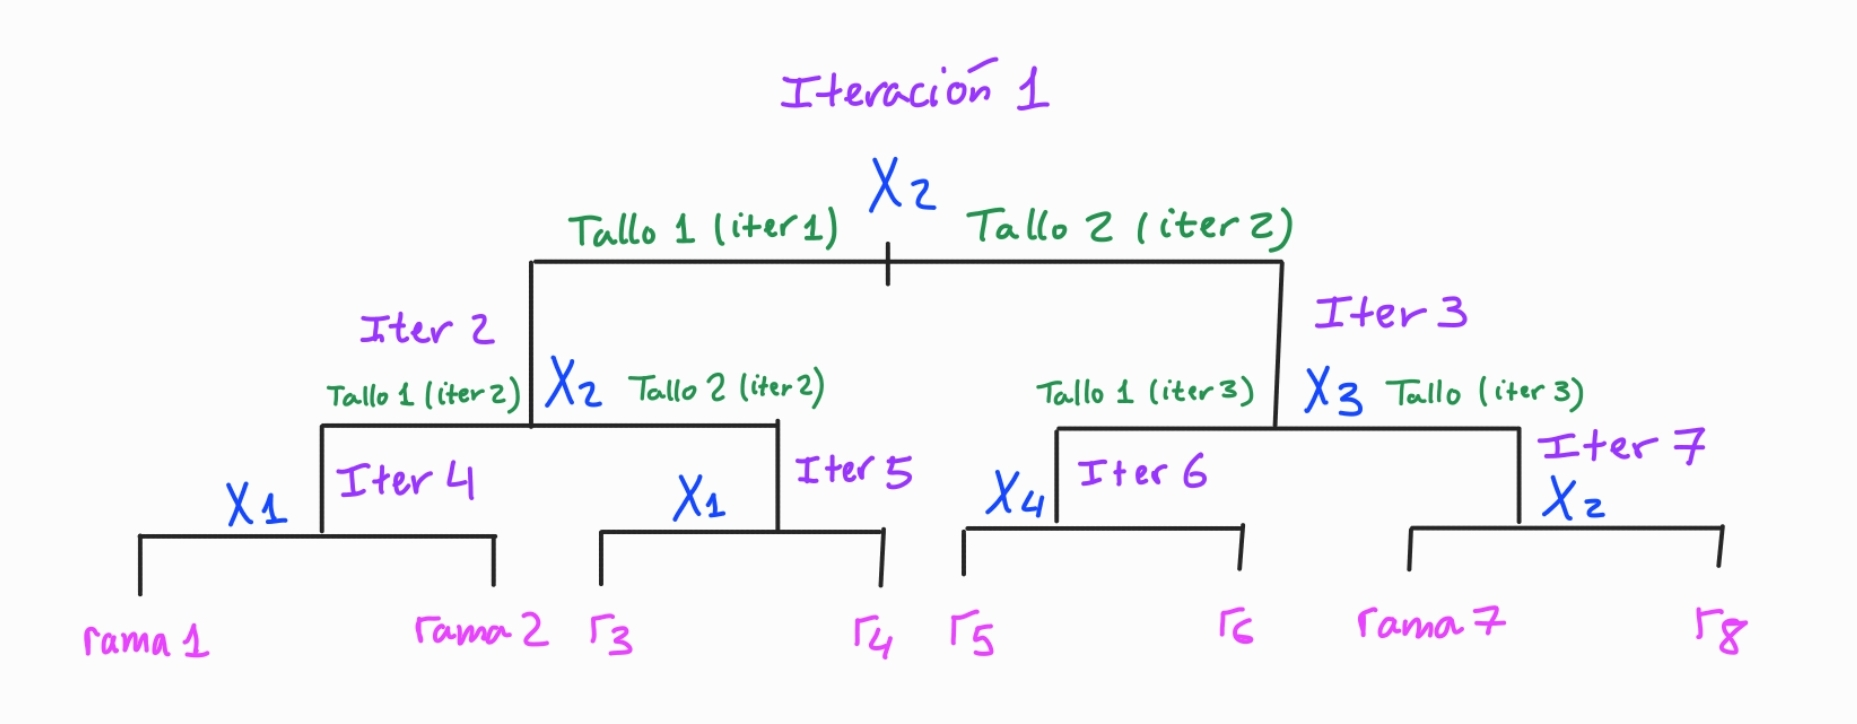
\includegraphics{output_397_0.jpg}
\caption{Arbol matemático}
\end{figure}

Es importante tener en cuenta los elementos que estan reflejados, pues
los usaremos posteriormente.

Los arboles estan compuestos de iteraciones, que a su vez cada una de
ellas se dividen en dos tallos. La union de tallos de distintas
iteraciones da lugar a las ramas del arbol.

\newpage

\hypertarget{definicion-formal-de-los-arboles-de-clasificaciuxf3n}{%
\subsubsection{Definicion formal de los arboles de
clasificación:}\label{definicion-formal-de-los-arboles-de-clasificaciuxf3n}}

La idea de los algoritmos de arboles de clasificacion es segmentar las
observaciones de los predictores \(X_1,...,X_p\) para predecir el valor
de la respuesta \(Y\) en base a esa informacion segmentada. Es algo asi
como predecir Y por grupos/segmentos.

\vspace{1cm}

\textbf{Elementos Básicos}

\begin{itemize}
\item
  Tenemos unos predictores \(\hspace{0.1cm} X_1,...,X_p \hspace{0.1cm}\)
  y una variable respuesta \textbf{categorica} \(\hspace{0.1cm} Y\)
\item
  Tenemos un arbol \(\hspace{0.1cm} T \hspace{0.1cm}\) de la forma del
  expuesto en la imagen con \(\hspace{0.1cm} m-1 \hspace{0.1cm}\)
  iteraciones y \(\hspace{0.1cm} m \hspace{0.1cm}\) ramas.
\item
  \(r_{ht}\) es la rama \(h\) del arbol con \(t\) iteraciones.
\item
  Cada iteracion del arbol tiene asociado uno de los predictores
  \(\hspace{0.07cm} X_1,...,X_n\)
\item
  Cada iteracion del arbol tiene dos tallos (tallo 1 (izquierdo) y tallo
  2 (derecho)).
\item
  En cada tallo de una iteracion se define un intervalo.
\item
  \(\hspace{0.1cm} I_{lt} \hspace{0.1cm}\) es el intervalo asociado al
  tallo \(l\) de la iteracion \(\hspace{0.1cm} t\)
\item
  Para simplificar el problema consideraremos
  \(\hspace{0.1cm} I_{1t} = (-\infty \hspace{0.03cm},\hspace{0.03cm} s_t)\hspace{0.1cm}\)
  y
  \(\hspace{0.1cm} I_{2t} = [s_t \hspace{0.03cm},\hspace{0.03cm} \infty]\hspace{0.1cm}\)
  donde \(\hspace{0.1cm} s_t \hspace{0.1cm}\) es llamado punto de corte
  de la iteracion \(\hspace{0.1cm} t \hspace{0.1cm}\) del arbol
\item
  \(R_{ht} \hspace{0.1cm}\) es la region (rectangulo \(n\)-dimensional)
  definida por la rama \(\hspace{0.1cm} h \hspace{0.1cm}\) de un arbol
  con \(t\) iteraciones
\end{itemize}

\newpage

\textbf{Criterio de prediccion de la variable respuesta}

Dada una nueva observacion
\(\hspace{0.1cm} x_{new}= (x_{new,1},x_{new,2},...,x_{new,p} ) \hspace{0.1cm}\)
la idea es predecir \(\hspace{0.1cm} y_{new} \hspace{0.1cm}\) como
sigue:

Sea \(\hspace{0.1 cm} f_{r, R_{ht}} \hspace{0.1 cm}\) la frecuencia
relativa de la clase/grupo r en la rama \(h\) de un arbol con \(t\)
iteraciones.

Es decir, es la proporcion de individuos de la muestra de entrenamiento
que caen en la rama \(h\) de un arbol con \(t\) iteraciones que
pertenecen a la clase \(r\) (es decir, para los que \(Y=r\) ) :

\[ \hspace{0.1 cm} f_{r , R_{ht}} \hspace{0.1 cm} = \hspace{0.1 cm} \dfrac{\# \hspace{0.1 cm}\lbrace i \hspace{0.1 cm}/\hspace{0.1 cm} x_i \in R_{ht} \hspace{0.15 cm}\text{y}\hspace{0.15 cm} y_i = r \rbrace}{\# \hspace{0.1 cm}\lbrace i \hspace{0.1 cm}/\hspace{0.1 cm} x_i \in R_{ht}  \rbrace} \]

\vspace{0.5cm}

Donde: \(\hspace{0.25cm} r \in Rango(Y) = \lbrace 0,1,..,c-1 \rbrace\)

\vspace{0.7cm}

\begin{itemize}
\tightlist
\item
  \(Si \hspace{0.3cm} x_{new} \in R_{ht} \hspace{0.15cm} \Rightarrow \hspace{0.15cm}\)
  \(x_{new}\) es clasificado en la clase/grupo mayoritaria (más
  frecuente) en la rama \(h\) \((r_h)\)
\end{itemize}

\vspace{0.5cm}

Por tanto:

\begin{itemize}
\tightlist
\item
  \(\hspace{0.4 cm} Si \hspace{0.22 cm} r_{R_{ht}}^* \hspace{0.05 cm}= \hspace{0.05 cm} \underset{\hspace{0.7 cm} r}{arg \hspace{0.1 cm} Max} \hspace{0.05 cm} \left(\hspace{0.1 cm} f_{r, R_{ht}} \hspace{0.1 cm}\right) \hspace{0.2 cm} ,\hspace{0.05 cm} entonces:\)
\end{itemize}

\[Si \hspace{0.3cm} x_{new} \in R_h \hspace{0.22cm}  \Rightarrow  \hspace{0.22cm}  \widehat{y}_{new} = r_{R_{ht}}^*\]

\vspace{0.7cm}

\emph{Observación:}

Definida la region \(\hspace{0.05 cm} R_{ht} \hspace{0.05 cm}\) , es
relativamente sencillo resolver el problema
\(\hspace{0.05 cm} \underset{ r}{ Max} \hspace{0.05 cm} \left(\hspace{0.1 cm} f_{r, R_{ht}} \hspace{0.1 cm}\right) \hspace{0.05 cm}\)
y asi obtener \(\hspace{0.05 cm} r_{R_{ht}}^*\)

\newpage

\textbf{Objetivo} : Usando la \textbf{tasa de error de clasificacion}
como métrica a optimizar

\vspace{0.35cm}

Definimos el \textbf{error de entrenamiento de la rama \(h\) de un arbol
de clasificacion con \(t\) iteraciones} como la tasa de error de
clasificacion para las observaciones de entrenamiento que caen en la
rama \(h\) de dicho arbol, es decir, como:

\[TEC(R_{ht}) = 1 - f_{r^*_{R_{ht}} , R_{ht}}\]

\vspace{0.35cm}

\emph{Observación:}

\(f_{r^*_{R_{ht}} , R_{ht}}\) es la proporcion de individuos de la
muestra de entrenamiento que caen en la rama \(h\) de un arbol con \(t\)
iteraciones que son de la clase/grupo \(r^*_{R_{ht}}\) (el valor de la
variable respuesta para ellos es \(r^*_{R_{ht}}\))

Como el modelo clasifica a los que caen en esa rama como de la clase
\(r^*_{R_{ht}}\) , es decir, como la predicion de la respuesta para todo
individuo que pertenezaca a esa rama es \(r^*_{R_{ht}}\) , por parte del
modelo, entonces se tiene lo siguiente:

\(f_{r^*_{R_{ht}} , R_{ht}}\) es la proporcion de individuos de la
muestra de entrenamiento que caen en la rama \(h\) de un arbol con \(t\)
iteraciones que son correctamente clasificados por el modelo (proporcion
de individuos de la region \(R_{ht}\) a los que se les ha predicho bien
la respuesta).

\(TEC(R_{ht})\) es la proporcion de individuos de la muestra de
entrenamiento que caen en la rama \(h\) de un arbol con \(t\)
iteraciones \((\) sus observaciones de los predictores pertenecen a
\(R_{ht}\) \()\) y que han sido clasificados erroneamente. Se les ha
clasificado en la clase \(r^*_{R_{ht}}\) y su clase era otra diferente,
es decir, tenian un valor distinto a \(r^*_{R_{ht}}\) para la variable
respeusta, que es el valor que el modelo les predice para la respuesta.

\vspace{0.35cm}

Definimos el \textbf{error global de entrenamiento de un arbol de
clasificación} como la suma de los errores de entrenamiento de las ramas
del arbol de clasificación:

\[\sum_{h=1}^{m} \hspace{0.1cm} TEC(R_h) \]

\vspace{0.35cm}

El \textbf{objetivo} es construir un arbol de regresion con \(m\) ramas
tal que \textbf{minimice} el \textbf{error global de entrenamiento}.

Es decir, formalmente el objetivo es:

\[ \underset{R_1,..,R_m}{Min}  \hspace{0.12cm}  \sum_{h=1}^{m} \hspace{0.1cm} TEC(R_h)  \]

\vspace{0.35cm}

Pero para escoger las regiones
\(\hspace{0.1cm} R_1,...,R_m \hspace{0.1cm}\) que definen las ramas del
arbol hay que determinar dos elementos que definen a su vez a las
regiones:

\(1.\hspace{0.1cm}\) Qué predictores estan asociados a cada iteracion
del arbol \(\hspace{0.1cm} \Rightarrow \hspace{0.1cm}\) Para cada
iteracion \(i\) escoger \(X_j \hspace{0.01cm}\) \$(\hspace{0.01cm} \$ es
decir, escoger \(j \hspace{0.01cm})\)

\(2.\hspace{0.1cm}\) Qué intervalos estan asociados a cada uno de los
dos tallos de cada interaccion
\(\hspace{0.1cm} \Rightarrow \hspace{0.1cm}\) Para cada iteracion \(i\)
escoger \(I_{1i}\) y \(I_{2i}\hspace{0.1cm}\) \((\hspace{0.01cm}\) es
decir, escoger el punto de corte
\(\hspace{0.07cm}s_i \hspace{0.04cm} )\)

Por tanto el porblema a resolver se puede reformular como:

Para cada iteracion \(\hspace{0.1cm} i \hspace{0.1cm}\) escoger
\(\hspace{0.1cm} X_j\hspace{0.01cm}\) \((\hspace{0.05cm}\) es decir
\(\hspace{0.01cm}j \hspace{0.05cm})\hspace{0.05cm}\) y
\(\hspace{0.05cm}( I_{1i}\hspace{0.1cm},\hspace{0.1cm}I_{2i} )\hspace{0.1cm}\)
\(\hspace{0.1cm}(\) es decir \(\hspace{0.1cm} s_i)\hspace{0.1cm}\) tal
que se acaben formando un arbol cuyas ramas definan unas regiones
\(\hspace{0.1cm}R_1,...,R_m\hspace{0.1cm}\) que \textbf{minimicen}
\(\hspace{0.1cm}\sum_{h=1}^{m} \hspace{0.1cm} TEC(R_h)\)

\vspace{1.5cm}

\textbf{Objetivo} : Usando el \textbf{índice de Gini} como métrica a
optimizar

\vspace{0.35cm}

Definimos el \textbf{error de entrenamiento de la rama \(h\) de un arbol
de clasificacion con \(t\) iteraciones} como el índice de Gini de la
respuesta en la rama \(h\) del arbol con \(t\) iteraciones (indice de
gini de la respuesta en la region \(R_{ht}\)) , es decir, como:

\[ G_{R_{ht}} = \sum_{r=0,1,..,c-1}^{} f_{r , R_{ht}}\cdot(1 - f_{r , R_{ht}}) \]

\vspace{0.35cm}

Donde: \(\hspace{0.15cm} Rango(Y) = \lbrace 0,1,...,c-1 \rbrace\)

\vspace{0.35cm}

\(G_{R_{ht}}\) toma valores pequeños cuando la frecuencia de una clase
\(r=0,1,...\) en la region \(R_{ht}\) es alta , y por tanto la del resto
baja.

\(G_{R_{ht}}\) toma valores altos cuando las frecuencias de las clases
se reparten de manera ``igualitaria'' en la region \(R_{ht}\). Y cuanto
mas igualitaria es la reparticion de las classes, mas alto es
\(G_{R_{ht}}\) . Hasta el punto que cuando la reparticion es totalmente
igualitaria, esto es, cada clase tiene la misma frecuencia , si hay
\(c\) clases, cada una tiene una frecuencia relativa de \(1/c\) en la
region, entonces en indicide de Gini alcanza su maximo valor.

\vspace{0.35cm}

\emph{Ejemplo:}

Para \(\hspace{0.1 cm} c=3\)
\(\hspace{0.15cm} ( Rango(Y)=\lbrace 0,1,2 \rbrace )\)

Si tenemos: \(\hspace{0.15cm} f_{0 , R_{ht}} = 0.40 \hspace{0.15cm}\) ,
\(\hspace{0.15cm} f_{1 , R_{ht}}=0.30 \hspace{0.15cm}\) y
\(\hspace{0.15cm} f_{2 , R_{ht}}=0.30\)
\(\hspace{0.15cm} \Rightarrow \hspace{0.15cm}\) \(G_{R_{ht}} = 0.66\)

Si tenemos: \(\hspace{0.15cm} f_{0 , R_{ht}} = 0.80 \hspace{0.15cm}\) ,
\(\hspace{0.15cm} f_{1 , R_{ht}}=0.10 \hspace{0.15cm}\) y
\(\hspace{0.15cm} f_{2 , R_{ht}}=0.10\)
\(\hspace{0.15cm} \Rightarrow \hspace{0.15cm}\) \(G_{R_{ht}} = 0.34\)

Si tenemos: \(\hspace{0.15cm} f_{0 , R_{ht}} = 0.9 \hspace{0.15cm}\) ,
\(\hspace{0.15cm} f_{1 , R_{ht}}=0.05 \hspace{0.15cm}\) y
\(\hspace{0.15cm} f_{2 , R_{ht}}=0.05\)
\(\hspace{0.15cm} \Rightarrow \hspace{0.15cm}\) \(G_{R_{ht}} = 0.185\)

\vspace{0.35cm}

Teniendo esto en cuenta nos interesan que en cada rama (region
\(R_{ht}\)) la frecuencia de la clase mayoritaria sea lo mayor posible,
y eso equivale a que el indice de Gini sea lo menos posible dentro de
cada rama, siguiendo la filosofia empleada con la \(TEC\), donde nos
interesaba que \(f_{r^*_{R_{ht}} , R_{ht}}\) fuese lo mayor posible en
cada rama.

\newpage

Definimos el \textbf{error global de entrenamiento de un arbol de
clasificación} como la suma de los errores de entrenamiento de las ramas
del arbol de clasificación:

\[\sum_{h=1}^{m} \hspace{0.1cm} G_{R_{ht}} \]

\vspace{0.35cm}

El \textbf{objetivo} es construir un arbol de regresion con \(m\) ramas
tal que \textbf{minimice} el \textbf{error global de entrenamiento}.

Es decir, formalmente el objetivo es:

\[ \underset{R_1,..,R_m}{Min}  \hspace{0.12cm}  \sum_{h=1}^{m} \hspace{0.1cm} G_{R_{ht}}  \]

\vspace{0.35cm}

En el fondo minimizar el error de clasificacion de un arbol de
clasificacion equivale a minimizar el indice de Gini en las ramas del
arbol conjuntamente (a nivel global).

\vspace{0.35cm}

Pero para escoger las regiones
\(\hspace{0.1cm} R_1,...,R_m \hspace{0.1cm}\) que definen las ramas del
arbol hay que determinar dos elementos que definen a su vez a las
regiones:

\(1.\hspace{0.1cm}\) Qué predictores estan asociados a cada iteracion
del arbol \(\hspace{0.1cm} \Rightarrow \hspace{0.1cm}\) Para cada
iteracion \(i\) escoger \(X_j \hspace{0.01cm}\) \$(\hspace{0.01cm} \$ es
decir, escoger \(j \hspace{0.01cm})\)

\(2.\hspace{0.1cm}\) Qué intervalos estan asociados a cada uno de los
dos tallos de cada interaccion
\(\hspace{0.1cm} \Rightarrow \hspace{0.1cm}\) Para cada iteracion \(i\)
escoger \(I_{1i}\) y \(I_{2i}\hspace{0.1cm}\) \((\hspace{0.01cm}\) es
decir, escoger el punto de corte
\(\hspace{0.07cm}s_i \hspace{0.04cm} )\)

\vspace{0.35cm}

Por tanto el porblema a resolver se puede reformular como:

Para cada iteracion \(\hspace{0.1cm} i \hspace{0.1cm}\) escoger
\(\hspace{0.1cm} X_j\hspace{0.01cm}\) \((\hspace{0.05cm}\) es decir
\(\hspace{0.01cm}j \hspace{0.05cm})\hspace{0.05cm}\) y
\(\hspace{0.05cm}( I_{1i}\hspace{0.1cm},\hspace{0.1cm}I_{2i} )\hspace{0.1cm}\)
\(\hspace{0.1cm}(\) es decir \(\hspace{0.1cm} s_i)\hspace{0.1cm}\) tal
que se acaben formando un arbol cuyas ramas definan unas regiones
\(\hspace{0.1cm}R_1,...,R_m\hspace{0.1cm}\) que \textbf{minimicen}
\(\hspace{0.1cm}\sum_{h=1}^{m} \hspace{0.1cm} G_{R_{ht}}\)

\newpage

\textbf{Algoritmo para la resolucion del problema : algoritmo de
particion binaria}

\vspace{0.2cm}

El siguiente algoritmo es una forma de resolver el problema planteado
anteriormente. Consiste en ir generando el arbol de manera secuencial,
iteracion a iteracion, minimizando en cada paso el error de
clasificacion para las observaciones de train que caen en las ramas
asociadas a la iteracion en cuestion que esta siendo optimizada.

El algoritmo se basa en la resolucion secuencial de problemas de
minimizacion, uno por cada iteracion tenga el arbol que se acabará
generando.

\vspace{0.5cm}

\textbf{Problema de la Iteración 1}

Arbol con 1 iteración:

\begin{figure}
\centering
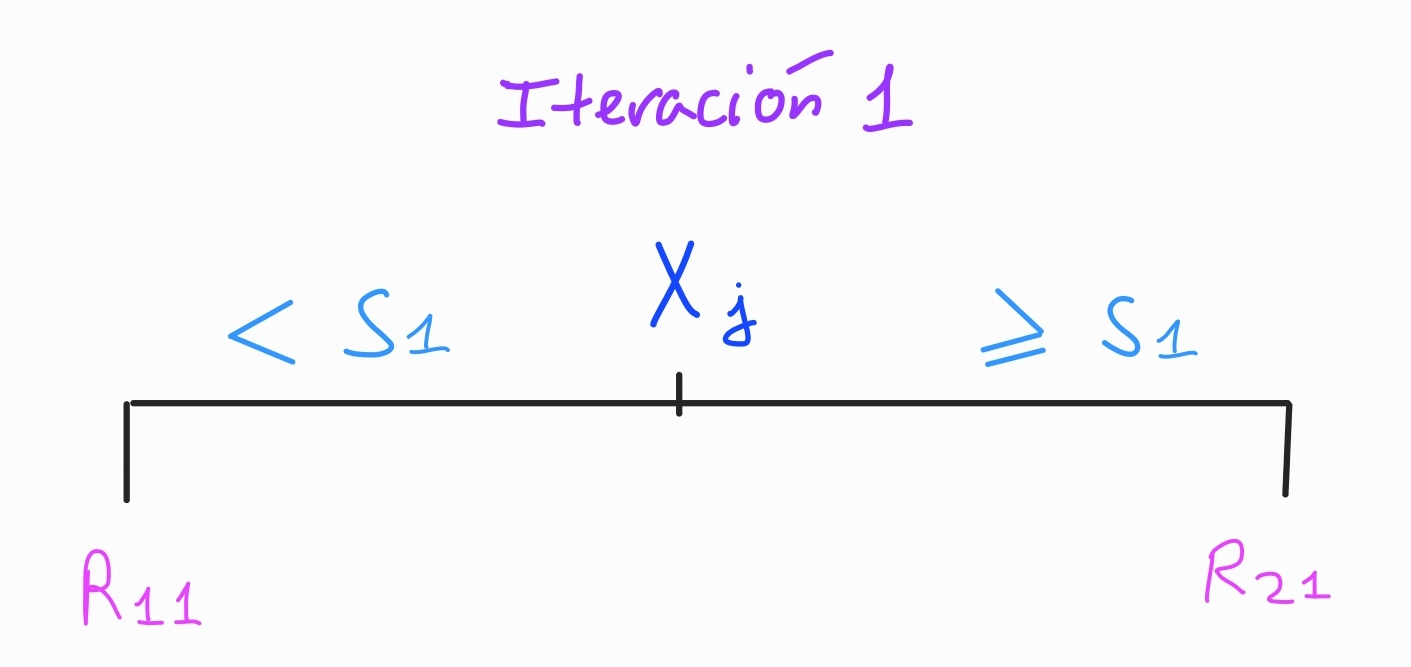
\includegraphics[width=4.375in,height=3.125in]{output_465_0.jpg}
\caption{Arbol 1ª Iteración}
\end{figure}

\vspace{0.5cm}

La idea es, determinar las regiones \(R_{11}\) y
\(R_{21}\hspace{0.1cm}\) \((\) es decir, \(j\) y
\(s_1 \hspace{0.05cm}) \hspace{0.1cm}\) del arbol con 1 iteracion tal
que minimizan el error de entrenamiento global de dicho arbol con 1
iteracion.

\vspace{0.5cm}

Mas formalmente el problema planteado es:

\begin{itemize}
\tightlist
\item
  Si utilizamos la \textbf{TEC} como metrica de error a minimizar:
\end{itemize}

\begin{gather*}
\underset{R_{11}  ,  R_{21}}  {Min} \hspace{0.15cm} \left(\hspace{0.1cm} TEC_1 = TEC(R_{11}) + TEC(R_{21})  \hspace{0.1cm}\right)   \hspace{0.1cm} =   \\ \\
=\hspace{0.2cm} \underset{R_{11}  ,  R_{21}}  {Min} \hspace{0.1cm} \left( \hspace{0.2cm}  \left( 1 - f_{r^*_{R_{11}} , R_{11}} \right)  \hspace{0.3cm} +  \hspace{0.1cm}    \left( 1 - f_{r^*_{R_{21}} , R_{21}} \right)  \hspace{0.2cm} \right)     \\ \\
=\hspace{0.2cm}   \underset{R_{11}  ,  R_{21}}  {Min} \hspace{0.1cm} \left( \hspace{0.2cm}    1 - \dfrac{\# \hspace{0.1 cm}\lbrace i \hspace{0.1 cm}/\hspace{0.1 cm} x_i \in R_{11} \hspace{0.15 cm}\text{y}\hspace{0.15 cm} y_i = r^*_{R_{11}} \rbrace}{\# \hspace{0.1 cm}\lbrace i \hspace{0.1 cm}/\hspace{0.1 cm} x_i \in R_{11}  \rbrace}  \hspace{0.3cm} +  \hspace{0.3cm}      1 - \dfrac{\# \hspace{0.1 cm}\lbrace i \hspace{0.1 cm}/\hspace{0.1 cm} x_i \in R_{21} \hspace{0.15 cm}\text{y}\hspace{0.15 cm} y_i = r^*_{R_{21}} \rbrace}{\# \hspace{0.1 cm}\lbrace i \hspace{0.1 cm}/\hspace{0.1 cm} x_i \in R_{21}  \rbrace}   \hspace{0.2cm} \right)     \\ \\
=\hspace{0.2cm}   \underset{j  ,  s_1}  {Min} \hspace{0.1cm} \left( \hspace{0.2cm}    1 - \dfrac{\# \hspace{0.1 cm}\lbrace i \hspace{0.1 cm}/\hspace{0.1 cm} x_i < s_1 \hspace{0.15 cm}\text{y}\hspace{0.15 cm} y_i = r^*_{R_{11}} \rbrace}{\# \hspace{0.1 cm}\lbrace i \hspace{0.1 cm}/\hspace{0.1 cm} x_i < s_1  \rbrace} \hspace{0.3cm} +  \hspace{0.3cm}      1 - \dfrac{\# \hspace{0.1 cm}\lbrace i \hspace{0.1 cm}/\hspace{0.1 cm} x_i \geqslant s_1 \hspace{0.15 cm}\text{y}\hspace{0.15 cm} y_i = r^*_{R_{21}} \rbrace}{\# \hspace{0.1 cm}\lbrace i \hspace{0.1 cm}/\hspace{0.1 cm} x_i \geqslant s_1 \rbrace}    \hspace{0.2cm} \right)    
\end{gather*}

\begin{itemize}
\tightlist
\item
  Si utilizamos el \textbf{índice de Gini} como metrica de error a
  minimizar:
\end{itemize}

\begin{gather*}
\underset{R_{11}  ,  R_{21}}  {Min} \hspace{0.15cm} \left(\hspace{0.1cm} G_1 = G_{R_{11}} + G_{R_{21}}  \hspace{0.1cm}\right)   \hspace{0.1cm} =   \\ \\
=\hspace{0.2cm} \underset{R_{11}  ,  R_{21}}  {Min} \hspace{0.1cm} \Biggl\{ \hspace{0.2cm}  \sum_{r=0,1,..,c-1}^{} f_{r , R_{11}}\cdot(1 - f_{r , R_{11}})  \hspace{0.1cm} + \hspace{0.1cm}  \sum_{r=0,1,..,c-1}^{} f_{r , R_{21}}\cdot(1 - f_{r , R_{21}})   \hspace{0.2cm} \Biggl\}     \\ \\ 
=\hspace{0.2cm}   \underset{R_{11}  ,  R_{21}}  {Min} \hspace{0.1cm} \Biggl\{\hspace{0.2cm}   \sum_{r=0,1,..,c-1}^{}  \dfrac{\# \hspace{0.1 cm}\lbrace i \hspace{0.1 cm}/\hspace{0.1 cm} x_i \in R_{11} \hspace{0.15 cm}\text{y}\hspace{0.15 cm} y_i = r  \rbrace}{\# \hspace{0.1 cm}\lbrace i \hspace{0.1 cm}/\hspace{0.1 cm} x_i \in R_{11}  \rbrace}  \cdot \left(   1 - \dfrac{\# \hspace{0.1 cm}\lbrace i \hspace{0.1 cm}/\hspace{0.1 cm} x_i \in R_{11} \hspace{0.15 cm}\text{y}\hspace{0.15 cm} y_i = r  \rbrace}{\# \hspace{0.1 cm}\lbrace i \hspace{0.1 cm}/\hspace{0.1 cm} x_i \in R_{11}  \rbrace}  \right) \\ \\
\hspace{0.3cm} +  \hspace{0.3cm}         \sum_{r=0,1,..,c-1}^{}  \dfrac{\# \hspace{0.1 cm}\lbrace i \hspace{0.1 cm}/\hspace{0.1 cm} x_i \in R_{21} \hspace{0.15 cm}\text{y}\hspace{0.15 cm} y_i = r  \rbrace}{\# \hspace{0.1 cm}\lbrace i \hspace{0.1 cm}/\hspace{0.1 cm} x_i \in R_{21}  \rbrace}  \cdot \left(   1 - \dfrac{\# \hspace{0.1 cm}\lbrace i \hspace{0.1 cm}/\hspace{0.1 cm} x_i \in R_{21} \hspace{0.15 cm}\text{y}\hspace{0.15 cm} y_i = r  \rbrace}{\# \hspace{0.1 cm}\lbrace i \hspace{0.1 cm}/\hspace{0.1 cm} x_i \in R_{21}  \rbrace}  \right)            \hspace{0.2cm} \Biggl\}     \\ \\
=\hspace{0.2cm}   \underset{j  ,  s_1}  {Min} \hspace{0.1cm} \Biggl\{     \sum_{r=0,1,..,c-1}^{}  \dfrac{\# \hspace{0.1 cm}\lbrace i \hspace{0.1 cm}/\hspace{0.1 cm} x_{ij} < s_1 \hspace{0.15 cm}\text{y}\hspace{0.15 cm} y_i = r  \rbrace}{\# \hspace{0.1 cm}\lbrace i \hspace{0.1 cm}/\hspace{0.1 cm} x_{ij} < s_1  \rbrace}  \cdot \left(   1 - \dfrac{\# \hspace{0.1 cm}\lbrace i \hspace{0.1 cm}/\hspace{0.1 cm} x_{ij} < s_1 \hspace{0.15 cm}\text{y}\hspace{0.15 cm} y_i = r  \rbrace}{\# \hspace{0.1 cm}\lbrace i \hspace{0.1 cm}/\hspace{0.1 cm} x_{ij} < s_1  \rbrace}  \right) \\ \\
\hspace{0.3cm} +  \hspace{0.3cm}         \sum_{r=0,1,..,c-1}^{}  \dfrac{\# \hspace{0.1 cm}\lbrace i \hspace{0.1 cm}/\hspace{0.1 cm} x_{ij} \geqslant s_1 \hspace{0.15 cm}\text{y}\hspace{0.15 cm} y_i = r \rbrace}{\# \hspace{0.1 cm}\lbrace i \hspace{0.1 cm}/\hspace{0.1 cm} x_{ij} \geqslant s_1 \rbrace}  \cdot \left(   1 - \dfrac{\# \hspace{0.1 cm}\lbrace i \hspace{0.1 cm}/\hspace{0.1 cm} x_{ij} \geqslant s_1 \hspace{0.15 cm}\text{y}\hspace{0.15 cm} y_i = r \rbrace}{\# \hspace{0.1 cm}\lbrace i \hspace{0.1 cm}/\hspace{0.1 cm} x_{ij} \geqslant s_1 \rbrace}  \right)           \Biggl\} 
\end{gather*}

\vspace{1.5cm}

Notar que:

\vspace{0.5cm}

\(R_{11} = \lbrace (v_1 ,..., v_n) / v_j < s_1 \rbrace \hspace{0.3cm}\Rightarrow\hspace{0.3cm} [\hspace{0.1cm} x_i \in R_{11} \hspace{0.1cm} \Leftrightarrow \hspace{0.1cm} x_{ij} < s_1 \hspace{0.1cm}] \hspace{0.3cm}\Rightarrow\hspace{0.3cm} \lbrace i/x_i \in R_{11} \rbrace = \lbrace i / x_{ij} < s_1 \rbrace\)

\(R_{21} = \lbrace (v_1 ,..., v_n) / v_j \geqslant s_1 \rbrace \hspace{0.3cm}\Rightarrow\hspace{0.3cm} [\hspace{0.1cm} x_i \in R_{21} \hspace{0.1cm} \Leftrightarrow \hspace{0.1cm} x_{ij} \geqslant s_1 \hspace{0.1cm}] \hspace{0.2cm}\Rightarrow\hspace{0.2cm} \lbrace i/x_i \in R_{11} \rbrace = \lbrace i / x_{ij} \geqslant s_1 \rbrace\)

\vspace{0.5cm}

Notese que determinar \(R_{11}\) y \(R_{21}\) es equivalente a
determinar el predictor \(X_j\) \((\) es decir \(j)\) y el punto de
corte \(s_1\) asociados a la Iteracion 1, ya que \(R_{11}\) y \(R_{21}\)
quedan determinadas al fijar \(X_j\) y \(s_1\)

\newpage

Notar también que:

\vspace{0.5cm}

Fijado \((j, s_1)\) puede calcularse \(r_{R_{11}}^*\) como solucion al
problema de maximizacion:

\[\underset{  r}{ Max} \hspace{0.05 cm} \left(\hspace{0.1 cm} f_{r, R_{11}} \hspace{0.1 cm}\right) = \underset{ r}{ Max} \hspace{0.05 cm} \left(\hspace{0.1 cm}   \dfrac{\# \hspace{0.1 cm}\lbrace i \hspace{0.1 cm}/\hspace{0.1 cm} x_i \in R_{11} \hspace{0.15 cm}\text{y}\hspace{0.15 cm} y_i = r \rbrace}{\# \hspace{0.1 cm}\lbrace i \hspace{0.1 cm}/\hspace{0.1 cm} x_i \in R_{11}  \rbrace}  \hspace{0.1 cm}\right) = \underset{  r}{ Max} \hspace{0.05 cm} \left(\hspace{0.1 cm}   \dfrac{\# \hspace{0.1 cm}\lbrace i \hspace{0.1 cm}/\hspace{0.1 cm} x_{ij} < s_1 \hspace{0.15 cm}\text{y}\hspace{0.15 cm} y_i = r \rbrace}{\# \hspace{0.1 cm}\lbrace i \hspace{0.1 cm}/\hspace{0.1 cm} x_{ij} < s_1 \rbrace}  \hspace{0.1 cm}\right)\]

Fijado \((j, s_2)\) puede calcularse \(r_{R_{21}}^*\) como solucion al
problema de maximizacion:

\[\underset{  r}{ Max} \hspace{0.05 cm} \left(\hspace{0.1 cm} f_{r, R_{21}} \hspace{0.1 cm}\right) = \underset{ r}{ Max} \hspace{0.05 cm} \left(\hspace{0.1 cm}   \dfrac{\# \hspace{0.1 cm}\lbrace i \hspace{0.1 cm}/\hspace{0.1 cm} x_i \in R_{21} \hspace{0.15 cm}\text{y}\hspace{0.15 cm} y_i = r \rbrace}{\# \hspace{0.1 cm}\lbrace i \hspace{0.1 cm}/\hspace{0.1 cm} x_i \in R_{21}  \rbrace}  \hspace{0.1 cm}\right) = \underset{  r}{ Max} \hspace{0.05 cm} \left(\hspace{0.1 cm}   \dfrac{\# \hspace{0.1 cm}\lbrace i \hspace{0.1 cm}/\hspace{0.1 cm} x_{ij} \geqslant s_1 \hspace{0.15 cm}\text{y}\hspace{0.15 cm} y_i = r \rbrace}{\# \hspace{0.1 cm}\lbrace i \hspace{0.1 cm}/\hspace{0.1 cm} x_{ij} \geqslant s_1 \rbrace}  \hspace{0.1 cm}\right)\]

\vspace{0.5cm}

Donde :

\begin{itemize}
\item
  \(\hspace{0.2cm} j \in \lbrace 1,2,...,p \rbrace\)
\item
  Si \(X_j\) es cuantitativa:
\end{itemize}

\(\hspace{0.7cm}\) Ordenamos las observaciones de \(X_j\) y quitamos
repeticiones, obtenemos \(X_j^{order}\), entonces:

\[  s_1 \in \Biggl\{ \dfrac{ x_{(1)j} + x_{(2)j} }{2} \hspace{0.1cm}, \hspace{0.1cm} \dfrac{x_{(2)j} + x_{(3)j} }{2} \hspace{0.1cm} ,...,\hspace{0.1cm} \dfrac{x_{(n-1)j} + x_{(n)j} }{2}   \Biggl\}\]

Donde \(\hspace{0.1cm} x_{(i)j} \hspace{0.1cm}\) es la observacion que
ocupa la posicion \(i\)-esima en \(\hspace{0.1cm} X_j^{order}\)

\begin{itemize}
\tightlist
\item
  Si \(X_j\) es categorica con \(c\) categorias:
\end{itemize}

\[ s_1 \in Rango(X_j) = \lbrace 0,1,..., c-1 \rbrace \]

\vspace{0.5cm}

Notese que la eleccion de \(X_j\) determina el campo de variacion de
\(s_1\)

\begin{itemize}
\item
  \(TEC(R_{11})\) es el error de entrenamiento de la rama \(1\) de un
  arbol de clasificación con 1 iteracion
\item
  \(TEC(R_{21})\) es el error de entrenamiento de la rama \(2\) de un
  arbol de clasificación con 1 iteracion
\end{itemize}

Estos elementos no volveran a ser definidos en los sucesivos problemas
de iteracion para no pecar de ser repetitivo, puesto que pueden ser
facilmente extrapolados a cualquier problema de iteracion. Ademas las
definiciones generales de estos elementos han sido expuestas ya
anteriormente.

\begin{itemize}
\tightlist
\item
  Denotaremos por
  \(\hspace{0.1cm} \left(\hspace{0.1cm} j^{*(i)} \hspace{0.05cm},\hspace{0.05cm} s^{*(i)} \hspace{0.1cm}\right) \hspace{0.1cm}\)
  a una solucion del problema de la Iteracion \(i\) , para
  \(i=1,...,m-1\)
\end{itemize}

\vspace{1.5cm}

Arbol obtenido tras resolver el problema de la Iteracion 1:

\begin{figure}
\centering
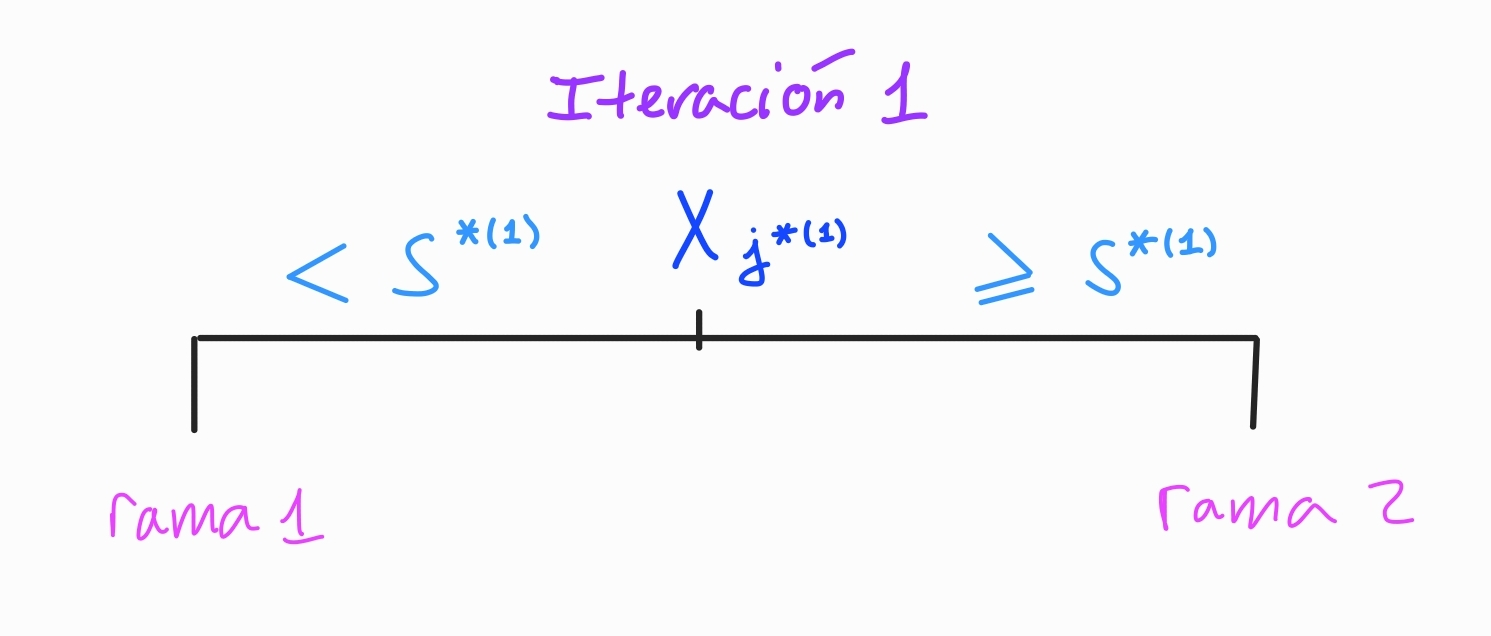
\includegraphics[width=4.375in,height=3.125in]{output_494_0.jpg}
\caption{Arbol óptimo tras resolver el problema de la 1ª Iteración}
\end{figure}

\begin{itemize}
\item
  Si alguna de las ramas del arbol resultante de resolver el problema la
  iteracion 1 tiene menos de \(\hspace{0.05cm}k\hspace{0.05cm}\)
  observaciones de train \(\hspace{0.1cm} \Rightarrow \hspace{0.1cm}\)
  se para el algoritmo
\item
  Si todas las ramas tienen \(\hspace{0.05cm}k\hspace{0.05cm}\) o mas
  observaciones de train \(\hspace{0.1cm} \Rightarrow \hspace{0.1cm}\)
  el algoritmo continua, se pasa a resolver el problema de la iteracion
  siguiente, en este caso el de la iteracion 2
\end{itemize}

Notese que \(k\) será un \textbf{\emph{hiperparametro}} del algoritmo.

\newpage

\textbf{Problema de la Iteracion 2}

Arbol con 2 iteraciones tras resolver el problema anterior:

\begin{figure}
\centering
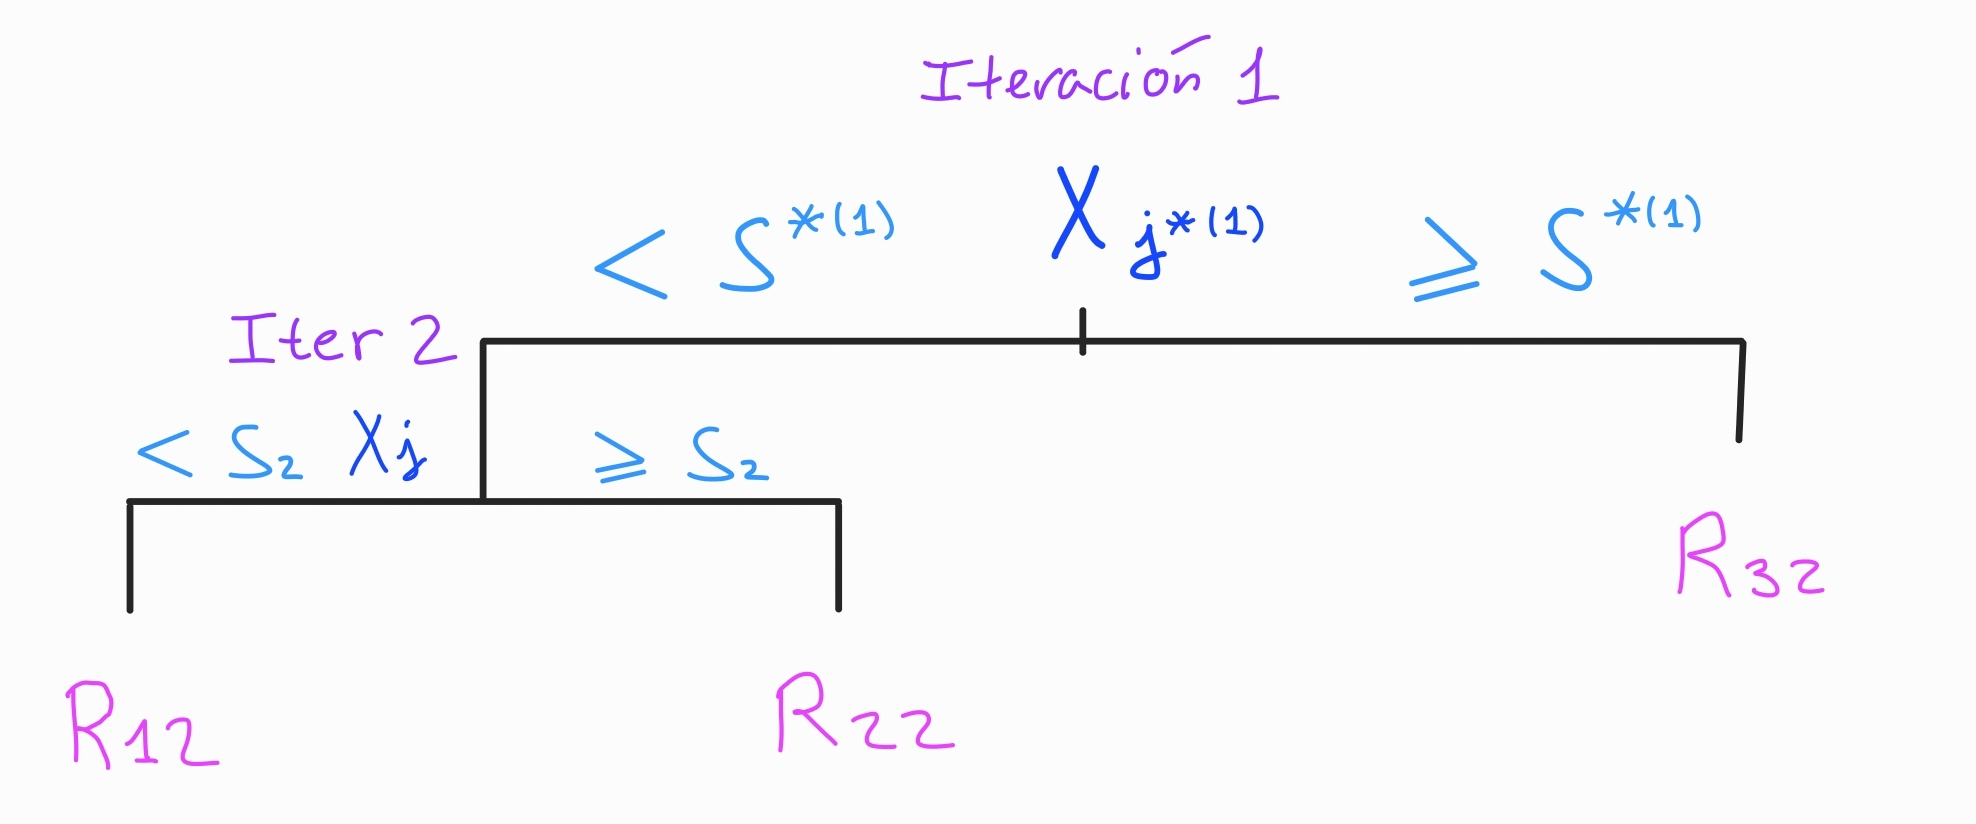
\includegraphics[width=4.375in,height=3.125in]{output_500_0.jpg}
\caption{Arbol con 2 Iteraciones tras resolver el problema de la 1ª
Iteración}
\end{figure}

\vspace{0.15cm}

Si estamos en este problema es porque ninguna rama del arbol resultante
del problema de la Iteracion 1 tiene menos de \(k\) observaciones

La idea es, determinar las regiones \(R_{12}\) , \(R_{22}\) y \(R_{32}\)
del arbol con 2 iteraciones (es decir, \(j\) y \(s_2\)), considerando la
solucion del problema de la iteracion 1 (arbol de arriba) , que
minimizan el error de entrenamiento global de dicho arbol.

Notese que \(R_{32}\) ya esta determinada tras la resolucion del
problema anterior, por ello realmente solo hay que determinar las
regiones \(R_{12}\) y \(R_{22}\) óptimas (a saber, \(j\) y \(s_2\)
óptimos)

\newpage

Mas formalmente el problema planteado es:

\begin{itemize}
\tightlist
\item
  Si utilizamos la \textbf{TEC} como metrica de error a minimizar:
\end{itemize}

\begin{gather*}
\underset{R_{12}  ,  R_{22},  R_{32}}  {Min} \hspace{0.15cm}  \Biggl\{ \hspace{0.1cm} TEC_2 = TEC(R_{12})  +  TEC(R_{22}) +  TEC(R_{32}) \hspace{0.1cm} \Biggl\}   \hspace{0.1cm} =   \\ \\
=\hspace{0.2cm} \underset{R_{12}  ,  R_{22}, R_{32}}  {Min} \hspace{0.1cm} \Biggl\{  \hspace{0.2cm}  \left( 1 - f_{r^*_{R_{12}} , R_{12}} \right)  \hspace{0.3cm} +  \hspace{0.1cm}       \left( 1 - f_{r^*_{R_{22}} , R_{22}} \right) \hspace{0.1cm} +  \hspace{0.1cm} \left( 1 - f_{r^*_{R_{32}} , R_{32}} \right)  \hspace{0.2cm}  \Biggl\}  \\ \\
=\hspace{0.2cm}   \underset{j \hspace{0.02cm},\hspace{0.02cm} s_2}  {Min} \hspace{0.1cm} \Biggl\{ \hspace{0.2cm}     1 - \dfrac{\# \hspace{0.1 cm}\lbrace i \hspace{0.1 cm}/\hspace{0.1 cm} x_i \in R_{12} \hspace{0.15 cm}\text{y}\hspace{0.15 cm} y_i = r^*_{R_{12}} \rbrace}{\# \hspace{0.1 cm}\lbrace i \hspace{0.1 cm}/\hspace{0.1 cm} x_i \in R_{12}  \rbrace}      \hspace{0.1cm} +  \hspace{0.1cm} 1 - \dfrac{\# \hspace{0.1 cm}\lbrace i \hspace{0.1 cm}/\hspace{0.1 cm} x_i \in R_{22} \hspace{0.15 cm}\text{y}\hspace{0.15 cm} y_i = r^*_{R_{22}} \rbrace}{\# \hspace{0.1 cm}\lbrace i \hspace{0.1 cm}/\hspace{0.1 cm} x_i \in R_{22}  \rbrace} \hspace{0.1cm} +    \hspace{0.1cm}   \\ \\ + \hspace{0.1 cm}   1 - \dfrac{\# \hspace{0.1 cm}\lbrace i \hspace{0.1 cm}/\hspace{0.1 cm} x_i \in R_{32} \hspace{0.15 cm}\text{y}\hspace{0.15 cm} y_i = r^*_{R_{32}} \rbrace}{\# \hspace{0.1 cm}\lbrace i \hspace{0.1 cm}/\hspace{0.1 cm} x_i \in R_{32}  \rbrace}  \hspace{0.2cm}  \Biggl\}   \\ \\
=\hspace{0.2cm}   \underset{j \hspace{0.02cm},\hspace{0.02cm} s_2}  {Min} \hspace{0.1cm} \Biggl\{ \hspace{0.2cm}     1 - \dfrac{\# \hspace{0.1 cm}\lbrace i \hspace{0.1 cm}/\hspace{0.1 cm}  x_{ij^{*(1)}} \hspace{0.05cm}   < \hspace{0.05cm} s^{*(1)} \hspace{0.25 cm}\text{y}\hspace{0.25 cm} x_{ij} \hspace{0.05cm}   < \hspace{0.05cm} s_2 \hspace{0.25 cm}\text{y}\hspace{0.25 cm} y_i = r^*_{R_{12}} \rbrace}{\# \hspace{0.1 cm}\lbrace i \hspace{0.1 cm} / \hspace{0.1 cm}  x_{ij^{*(1)}} \hspace{0.05cm}   < \hspace{0.05cm} s^{*(1)} \hspace{0.25 cm}\text{y}\hspace{0.25 cm} x_{ij} \hspace{0.05cm}   < \hspace{0.05cm} s_2  \hspace{0.1 cm} \rbrace }      \hspace{0.3cm} + 
\\  \\
1 -  \dfrac{\# \hspace{0.1 cm}\lbrace i \hspace{0.1 cm}/\hspace{0.1 cm}  x_{ij^{*(1)}} \hspace{0.05cm}   < \hspace{0.05cm} s^{*(1)} \hspace{0.25 cm}\text{y}\hspace{0.25 cm} x_{ij} \hspace{0.05cm}   \geqslant \hspace{0.05cm} s_2 \hspace{0.25 cm}\text{y}\hspace{0.25 cm} y_i = r^*_{R_{22}} \rbrace}{\# \hspace{0.1 cm}\lbrace i \hspace{0.1 cm} / \hspace{0.1 cm}  x_{ij^{*(1)}} \hspace{0.05cm}   < \hspace{0.05cm} s^{*(1)} \hspace{0.25 cm}\text{y}\hspace{0.25 cm} x_{ij} \hspace{0.05cm}   \geqslant \hspace{0.05cm} s_2  \hspace{0.1 cm} \rbrace } \hspace{0.3cm} +  \\ \\
1 - \dfrac{\# \hspace{0.1 cm}\lbrace i \hspace{0.1 cm}/\hspace{0.1 cm} x_{ij^{*(1)}} \geqslant s^{*(1)} \hspace{0.15 cm}\text{y}\hspace{0.15 cm} y_i = r^*_{R_{32}} \rbrace}{\# \hspace{0.1 cm}\lbrace i \hspace{0.1 cm}/\hspace{0.1 cm} x_{ij^{*(1)}} \geqslant s^{*(1)} \rbrace}  \hspace{0.2cm}  \Biggl\}
\\ \\  =\hspace{0.2cm}   \underset{j \hspace{0.02cm},\hspace{0.02cm} s_2}  {Min} \hspace{0.1cm} \Biggl\{   \hspace{0.2cm}    1 - \dfrac{\# \hspace{0.1 cm}\lbrace i \hspace{0.1 cm}/\hspace{0.1 cm}  x_{ij^{*(1)}} \hspace{0.05cm}   < \hspace{0.05cm} s^{*(1)} \hspace{0.25 cm}\text{y}\hspace{0.25 cm} x_{ij} \hspace{0.05cm}   < \hspace{0.05cm} s_2 \hspace{0.25 cm}\text{y}\hspace{0.25 cm} y_i = r^*_{R_{12}} \rbrace}{\# \hspace{0.1 cm}\lbrace i \hspace{0.1 cm} / \hspace{0.1 cm}  x_{ij^{*(1)}} \hspace{0.05cm}   < \hspace{0.05cm} s^{*(1)} \hspace{0.25 cm}\text{y}\hspace{0.25 cm} x_{ij} \hspace{0.05cm}   < \hspace{0.05cm} s_2  \hspace{0.1 cm} \rbrace }      \hspace{0.4cm} + \\ \\
\hspace{0.4cm}   1 -  \dfrac{\# \hspace{0.1 cm}\lbrace i \hspace{0.1 cm}/\hspace{0.1 cm}  x_{ij^{*(1)}} \hspace{0.05cm}   < \hspace{0.05cm} s^{*(1)} \hspace{0.25 cm}\text{y}\hspace{0.25 cm} x_{ij} \hspace{0.05cm}   \geqslant \hspace{0.05cm} s_2 \hspace{0.25 cm}\text{y}\hspace{0.25 cm} y_i = r^*_{R_{22}} \rbrace}{\# \hspace{0.1 cm}\lbrace i \hspace{0.1 cm} / \hspace{0.1 cm}  x_{ij^{*(1)}} \hspace{0.05cm}   < \hspace{0.05cm} s^{*(1)} \hspace{0.25 cm}\text{y}\hspace{0.25 cm} x_{ij} \hspace{0.05cm}   \geqslant \hspace{0.05cm} s_2  \hspace{0.1 cm} \rbrace }    \hspace{0.2cm}  \Biggl\} \\  \\
=\hspace{0.2cm} \underset{R_{12}  ,  R_{22} }  {Min} \hspace{0.1cm} \Biggl\{  \hspace{0.2cm}  \left( 1 - f_{r^*_{R_{12}} , R_{12}} \right)  \hspace{0.3cm} +  \hspace{0.1cm}       \left( 1 - f_{r^*_{R_{22}} , R_{22}} \right)   \hspace{0.2cm}  \Biggl\}
\end{gather*}

\newpage

\begin{itemize}
\tightlist
\item
  Si utilizamos el \textbf{índice de Gini} como metrica de error a
  minimizar:
\end{itemize}

\begin{gather*}
\underset{R_{12}  ,  R_{22}, R_{32}}  {Min} \hspace{0.15cm} \Biggl\{  \hspace{0.1cm} G_1 = G_{R_{12}} + G_{R_{22}} +  G_{R_{32}}  \hspace{0.1cm} \Biggl\}    \hspace{0.1cm} =   \\ \\ 
=\hspace{0.2cm} \underset{R_{12}  ,  R_{22}, R_{32}}  {Min} \hspace{0.1cm} \Biggl\{ \hspace{0.3cm}  \sum_{r=0,1,..,c-1}^{} f_{r , R_{12}}\cdot(1 - f_{r , R_{12}})  \hspace{0.1cm} + \hspace{0.1cm}  \sum_{r=0,1,..,c-1}^{} f_{r , R_{22}}\cdot(1 - f_{r , R_{22}}) \hspace{0.1cm} + \\ \\
\hspace{0.1cm}  \sum_{r=0,1,..,c-1}^{} f_{r , R_{32}}\cdot(1 - f_{r , R_{32}})  \hspace{0.3cm} \Biggl\} =     \\ \\
=\hspace{0.2cm}   \underset{R_{12}  ,  R_{22}  ,  R_{32}}  {Min} \hspace{0.1cm} \Biggl\{ \hspace{0.3cm}   \sum_{r=0,1,..,c-1}^{}  \dfrac{\# \hspace{0.1 cm}\lbrace i \hspace{0.1 cm}/\hspace{0.1 cm} x_i \in R_{12} \hspace{0.15 cm}\text{y}\hspace{0.15 cm} y_i = r  \rbrace}{\# \hspace{0.1 cm}\lbrace i \hspace{0.1 cm}/\hspace{0.1 cm} x_i \in R_{12}  \rbrace}  \cdot \left(   1 - \dfrac{\# \hspace{0.1 cm}\lbrace i \hspace{0.1 cm}/\hspace{0.1 cm} x_i \in R_{12} \hspace{0.15 cm}\text{y}\hspace{0.15 cm} y_i = r  \rbrace}{\# \hspace{0.1 cm}\lbrace i \hspace{0.1 cm}/\hspace{0.1 cm} x_i \in R_{12}  \rbrace}  \right)  \\ \\ 
\hspace{0.3cm} +  \hspace{0.3cm}         \sum_{r=0,1,..,c-1}^{}  \dfrac{\# \hspace{0.1 cm}\lbrace i \hspace{0.1 cm}/\hspace{0.1 cm} x_i \in R_{22} \hspace{0.15 cm}\text{y}\hspace{0.15 cm} y_i = r  \rbrace}{\# \hspace{0.1 cm}\lbrace i \hspace{0.1 cm}/\hspace{0.1 cm} x_i \in R_{22}  \rbrace}  \cdot \left(   1 - \dfrac{\# \hspace{0.1 cm}\lbrace i \hspace{0.1 cm}/\hspace{0.1 cm} x_i \in R_{22} \hspace{0.15 cm}\text{y}\hspace{0.15 cm} y_i = r  \rbrace}{\# \hspace{0.1 cm}\lbrace i \hspace{0.1 cm}/\hspace{0.1 cm} x_i \in R_{22}  \rbrace}  \right)    \\ \\
\hspace{0.3cm} +  \hspace{0.3cm}  \sum_{r=0,1,..,c-1}^{}  \dfrac{\# \hspace{0.1 cm}\lbrace i \hspace{0.1 cm}/\hspace{0.1 cm} x_i \in R_{32} \hspace{0.15 cm}\text{y}\hspace{0.15 cm} y_i = r  \rbrace}{\# \hspace{0.1 cm}\lbrace i \hspace{0.1 cm}/\hspace{0.1 cm} x_i \in R_{32}  \rbrace}  \cdot \left(   1 - \dfrac{\# \hspace{0.1 cm}\lbrace i \hspace{0.1 cm}/\hspace{0.1 cm} x_i \in R_{32} \hspace{0.15 cm}\text{y}\hspace{0.15 cm} y_i = r  \rbrace}{\# \hspace{0.1 cm}\lbrace i \hspace{0.1 cm}/\hspace{0.1 cm} x_i \in R_{32}  \rbrace}  \right)    \hspace{0.3cm} \Biggl\} =    \\ \\ 
 \hspace{-2.5 cm}=     \underset{j  ,  s_2}  {Min} \Biggl\{     \hspace{0.3cm}  \sum_{r=0,1,..,c-1}^{}   \dfrac{\# \hspace{0.1 cm}\lbrace i \hspace{0.1 cm}/\hspace{0.1 cm}  x_{ij^{*(1)}} \hspace{0.05cm}   < \hspace{0.05cm} s^{*(1)} \hspace{0.25 cm}\text{y}\hspace{0.25 cm} x_{ij} \hspace{0.05cm}   < \hspace{0.05cm} s_2 \hspace{0.25 cm}\text{y}\hspace{0.25 cm} y_i = r \rbrace}{\# \hspace{0.1 cm}\lbrace i \hspace{0.1 cm} / \hspace{0.1 cm}  x_{ij^{*(1)}} \hspace{0.05cm}   < \hspace{0.05cm} s^{*(1)} \hspace{0.25 cm}\text{y}\hspace{0.25 cm} x_{ij} \hspace{0.05cm}   < \hspace{0.05cm} s_2  \hspace{0.1 cm} \rbrace } \cdot 
\left(   1 -  \dfrac{\# \hspace{0.1 cm}\lbrace i \hspace{0.1 cm}/\hspace{0.1 cm}  x_{ij^{*(1)}} \hspace{0.05cm}   < \hspace{0.05cm} s^{*(1)} \hspace{0.25 cm}\text{y}\hspace{0.25 cm} x_{ij} \hspace{0.05cm}   < \hspace{0.05cm} s_2 \hspace{0.25 cm}\text{y}\hspace{0.25 cm} y_i = r \rbrace}{\# \hspace{0.1 cm}\lbrace i \hspace{0.1 cm} / \hspace{0.1 cm}  x_{ij^{*(1)}} \hspace{0.05cm}   < \hspace{0.05cm} s^{*(1)} \hspace{0.25 cm}\text{y}\hspace{0.25 cm} x_{ij} \hspace{0.05cm}   < \hspace{0.05cm} s_2  \hspace{0.1 cm} \rbrace } \right) \\ \\ 
\hspace{-1.5 cm} +  \hspace{0.3cm}         \sum_{r=0,1,..,c-1}^{}  \dfrac{\# \hspace{0.1 cm}\lbrace i \hspace{0.1 cm}/\hspace{0.1 cm}  x_{ij^{*(1)}} \hspace{0.05cm}   < \hspace{0.05cm} s^{*(1)} \hspace{0.25 cm}\text{y}\hspace{0.25 cm} x_{ij} \hspace{0.05cm}   \geqslant \hspace{0.05cm} s_2 \hspace{0.25 cm}\text{y}\hspace{0.25 cm} y_i = r \rbrace}{\# \hspace{0.1 cm}\lbrace i \hspace{0.1 cm} / \hspace{0.1 cm}  x_{ij^{*(1)}} \hspace{0.05cm}   < \hspace{0.05cm} s^{*(1)} \hspace{0.25 cm}\text{y}\hspace{0.25 cm} x_{ij} \hspace{0.05cm}   \geqslant \hspace{0.05cm} s_2  \hspace{0.1 cm} \rbrace }  \cdot \left(   1 - \dfrac{\# \hspace{0.1 cm}\lbrace i \hspace{0.1 cm}/\hspace{0.1 cm}  x_{ij^{*(1)}} \hspace{0.05cm}   < \hspace{0.05cm} s^{*(1)} \hspace{0.25 cm}\text{y}\hspace{0.25 cm} x_{ij} \hspace{0.05cm}   \geqslant \hspace{0.05cm} s_2 \hspace{0.25 cm}\text{y}\hspace{0.25 cm} y_i = r \rbrace}{\# \hspace{0.1 cm}\lbrace i \hspace{0.1 cm} / \hspace{0.1 cm}  x_{ij^{*(1)}} \hspace{0.05cm}   < \hspace{0.05cm} s^{*(1)} \hspace{0.25 cm}\text{y}\hspace{0.25 cm} x_{ij} \hspace{0.05cm}   \geqslant \hspace{0.05cm} s_2  \hspace{0.1 cm} \rbrace }  \right)  \\ \\
 +  \hspace{0.3cm}         \sum_{r=0,1,..,c-1}^{}  \dfrac{\# \hspace{0.1 cm}\lbrace i \hspace{0.1 cm}/\hspace{0.1 cm} x_{ij^{*(1)}} \geqslant s^{*(1)} \hspace{0.15 cm}\text{y}\hspace{0.15 cm} y_i = r \rbrace}{\# \hspace{0.1 cm}\lbrace i \hspace{0.1 cm}/\hspace{0.1 cm} x_{ij^{*(1)}} \geqslant s^{*(1)} \rbrace}  \cdot \left(   1 - \dfrac{\# \hspace{0.1 cm}\lbrace i \hspace{0.1 cm}/\hspace{0.1 cm} x_{ij^{*(1)}} \geqslant s^{*(1)} \hspace{0.15 cm}\text{y}\hspace{0.15 cm} y_i = r \rbrace}{\# \hspace{0.1 cm}\lbrace i \hspace{0.1 cm}/\hspace{0.1 cm} x_{ij^{*(1)}} \geqslant s^{*(1)} \rbrace}  \right)      \hspace{0.3cm}       \Biggl\}  
\end{gather*}

\begin{gather*}
\hspace{-2.5 cm} =     \underset{j  ,  s_2}  {Min} \hspace{0.1cm} \Biggl\{     \hspace{0.3cm}  \sum_{r=0,1,..,c-1}^{}   \dfrac{\# \hspace{0.1 cm}\lbrace i \hspace{0.1 cm}/\hspace{0.1 cm}  x_{ij^{*(1)}} \hspace{0.05cm}   < \hspace{0.05cm} s^{*(1)} \hspace{0.25 cm}\text{y}\hspace{0.25 cm} x_{ij} \hspace{0.05cm}   < \hspace{0.05cm} s_2 \hspace{0.25 cm}\text{y}\hspace{0.25 cm} y_i = r \rbrace}{\# \hspace{0.1 cm}\lbrace i \hspace{0.1 cm} / \hspace{0.1 cm}  x_{ij^{*(1)}} \hspace{0.05cm}   < \hspace{0.05cm} s^{*(1)} \hspace{0.25 cm}\text{y}\hspace{0.25 cm} x_{ij} \hspace{0.05cm}   < \hspace{0.05cm} s_2  \hspace{0.1 cm} \rbrace } \cdot \left(   1 -  \dfrac{\# \hspace{0.1 cm}\lbrace i \hspace{0.1 cm}/\hspace{0.1 cm}  x_{ij^{*(1)}} \hspace{0.05cm}   < \hspace{0.05cm} s^{*(1)} \hspace{0.25 cm}\text{y}\hspace{0.25 cm} x_{ij} \hspace{0.05cm}   < \hspace{0.05cm} s_2 \hspace{0.25 cm}\text{y}\hspace{0.25 cm} y_i = r \rbrace}{\# \hspace{0.1 cm}\lbrace i \hspace{0.1 cm} / \hspace{0.1 cm}  x_{ij^{*(1)}} \hspace{0.05cm}   < \hspace{0.05cm} s^{*(1)} \hspace{0.25 cm}\text{y}\hspace{0.25 cm} x_{ij} \hspace{0.05cm}   < \hspace{0.05cm} s_2  \hspace{0.1 cm} \rbrace } \right) \\ \\
\hspace{-1.5 cm} +  \hspace{0.1cm}         \sum_{r=0,1,..,c-1}^{}  \dfrac{\# \hspace{0.1 cm}\lbrace i \hspace{0.1 cm}/\hspace{0.1 cm}  x_{ij^{*(1)}} \hspace{0.05cm}   < \hspace{0.05cm} s^{*(1)} \hspace{0.25 cm}\text{y}\hspace{0.25 cm} x_{ij} \hspace{0.05cm}   \geqslant \hspace{0.05cm} s_2 \hspace{0.25 cm}\text{y}\hspace{0.25 cm} y_i = r \rbrace}{\# \hspace{0.1 cm}\lbrace i \hspace{0.1 cm} / \hspace{0.1 cm}  x_{ij^{*(1)}} \hspace{0.05cm}   < \hspace{0.05cm} s^{*(1)} \hspace{0.25 cm}\text{y}\hspace{0.25 cm} x_{ij} \hspace{0.05cm}   \geqslant \hspace{0.05cm} s_2  \hspace{0.1 cm} \rbrace }  \cdot \left(   1 - \dfrac{\# \hspace{0.1 cm}\lbrace i \hspace{0.1 cm}/\hspace{0.1 cm}  x_{ij^{*(1)}} \hspace{0.05cm}   < \hspace{0.05cm} s^{*(1)} \hspace{0.25 cm}\text{y}\hspace{0.25 cm} x_{ij} \hspace{0.05cm}   \geqslant \hspace{0.05cm} s_2 \hspace{0.25 cm}\text{y}\hspace{0.25 cm} y_i = r \rbrace}{\# \hspace{0.1 cm}\lbrace i \hspace{0.1 cm} / \hspace{0.1 cm}  x_{ij^{*(1)}} \hspace{0.05cm}   < \hspace{0.05cm} s^{*(1)} \hspace{0.25 cm}\text{y}\hspace{0.25 cm} x_{ij} \hspace{0.05cm}   \geqslant \hspace{0.05cm} s_2  \hspace{0.1 cm} \rbrace }  \right)    \Biggl\} \\ \\
\hspace{-1.5 cm} =   \underset{R_{12}  ,  R_{22} }  {Min} \hspace{0.1cm} \Biggl\{ \hspace{0.3cm}  \sum_{r=0,1,..,c-1}^{} f_{r , R_{12}}\cdot(1 - f_{r , R_{12}})  \hspace{0.1cm} + \hspace{0.1cm}  \sum_{r=0,1,..,c-1}^{} f_{r , R_{22}}\cdot(1 - f_{r , R_{22}})  \hspace{0.3cm} \Biggl\}  
\end{gather*}

Notar que:

Fijado \((j, s_2)\) puede calcularse \(r_{R_{12}}^*\) como solucion al
problema de maximizacion:

\begin{gather*}
\underset{  r}{ Max} \hspace{0.05 cm} \left(\hspace{0.1 cm} f_{r, R_{12}} \hspace{0.1 cm}\right) = \underset{ r}{ Max} \hspace{0.05 cm} \left(\hspace{0.1 cm}   \dfrac{\# \hspace{0.1 cm}\lbrace i \hspace{0.1 cm}/\hspace{0.1 cm} x_i \in R_{12} \hspace{0.15 cm}\text{y}\hspace{0.15 cm} y_i = r \rbrace}{\# \hspace{0.1 cm}\lbrace i \hspace{0.1 cm}/\hspace{0.1 cm} x_i \in R_{12}  \rbrace}  \hspace{0.1 cm}\right) = \\ \\ \underset{  r}{ Max} \hspace{0.05 cm} \left(\hspace{0.1 cm}   \dfrac{\# \hspace{0.1 cm}\lbrace i \hspace{0.1 cm}/\hspace{0.1 cm}  x_{ij^{*(1)}} \hspace{0.05cm}   < \hspace{0.05cm} s^{*(1)} \hspace{0.25 cm}\text{y}\hspace{0.25 cm} x_{ij} \hspace{0.05cm}   < \hspace{0.05cm} s_2 \hspace{0.25 cm}\text{y}\hspace{0.25 cm} y_i = r \rbrace}{\# \hspace{0.1 cm}\lbrace i \hspace{0.1 cm} / \hspace{0.1 cm}  x_{ij^{*(1)}} \hspace{0.05cm}   < \hspace{0.05cm} s^{*(1)} \hspace{0.25 cm}\text{y}\hspace{0.25 cm} x_{ij} \hspace{0.05cm}   < \hspace{0.05cm} s_2  \hspace{0.1 cm} \rbrace }\right)
\end{gather*}

\vspace{0.35cm}

Fijado \((j, s_2)\) puede calcularse \(r_{R_{22}}^*\) como solucion al
problema de maximizacion:

\begin{gather*}
\underset{  r}{ Max} \hspace{0.05 cm} \left(\hspace{0.1 cm} f_{r, R_{22}} \hspace{0.1 cm}\right) = \underset{ r}{ Max} \hspace{0.05 cm} \left(\hspace{0.1 cm}   \dfrac{\# \hspace{0.1 cm}\lbrace i \hspace{0.1 cm}/\hspace{0.1 cm} x_i \in R_{22} \hspace{0.15 cm}\text{y}\hspace{0.15 cm} y_i = r \rbrace}{\# \hspace{0.1 cm}\lbrace i \hspace{0.1 cm}/\hspace{0.1 cm} x_i \in R_{22}  \rbrace}  \hspace{0.1 cm}\right) = \\ \\ \underset{  r}{ Max} \hspace{0.05 cm} \left(\hspace{0.1 cm}   \dfrac{\# \hspace{0.1 cm}\lbrace i \hspace{0.1 cm}/\hspace{0.1 cm}  x_{ij^{*(1)}} \hspace{0.05cm}   < \hspace{0.05cm} s^{*(1)} \hspace{0.25 cm}\text{y}\hspace{0.25 cm} x_{ij} \hspace{0.05cm}   \geqslant \hspace{0.05cm} s_2 \hspace{0.25 cm}\text{y}\hspace{0.25 cm} y_i = r \rbrace}{\# \hspace{0.1 cm}\lbrace i \hspace{0.1 cm} / \hspace{0.1 cm}  x_{ij^{*(1)}} \hspace{0.05cm}   < \hspace{0.05cm} s^{*(1)} \hspace{0.25 cm}\text{y}\hspace{0.25 cm} x_{ij} \hspace{0.05cm}   \geqslant \hspace{0.05cm} s_2  \hspace{0.1 cm} \rbrace } \right)
\end{gather*}

\vspace{0.35cm}

Notese que ninguna de las siguientes expresiones:

\[\left( 1 - f_{r^*_{R_{32}} , R_{32}} \right)\]

\[\sum_{r=0,1,..,c-1}^{} f_{r , R_{32}}\cdot(1 - f_{r , R_{32}})\]

dependen de \((j, s_2)\) , por lo que puede sacarse de la funcion
objetivo de sus respectivos problemas de minimizacion sin que esto
altere la solucion del problema.

\vspace{0.35cm}

Arbol tras resolver el problema de la Iteración 2:

\begin{figure}
\centering
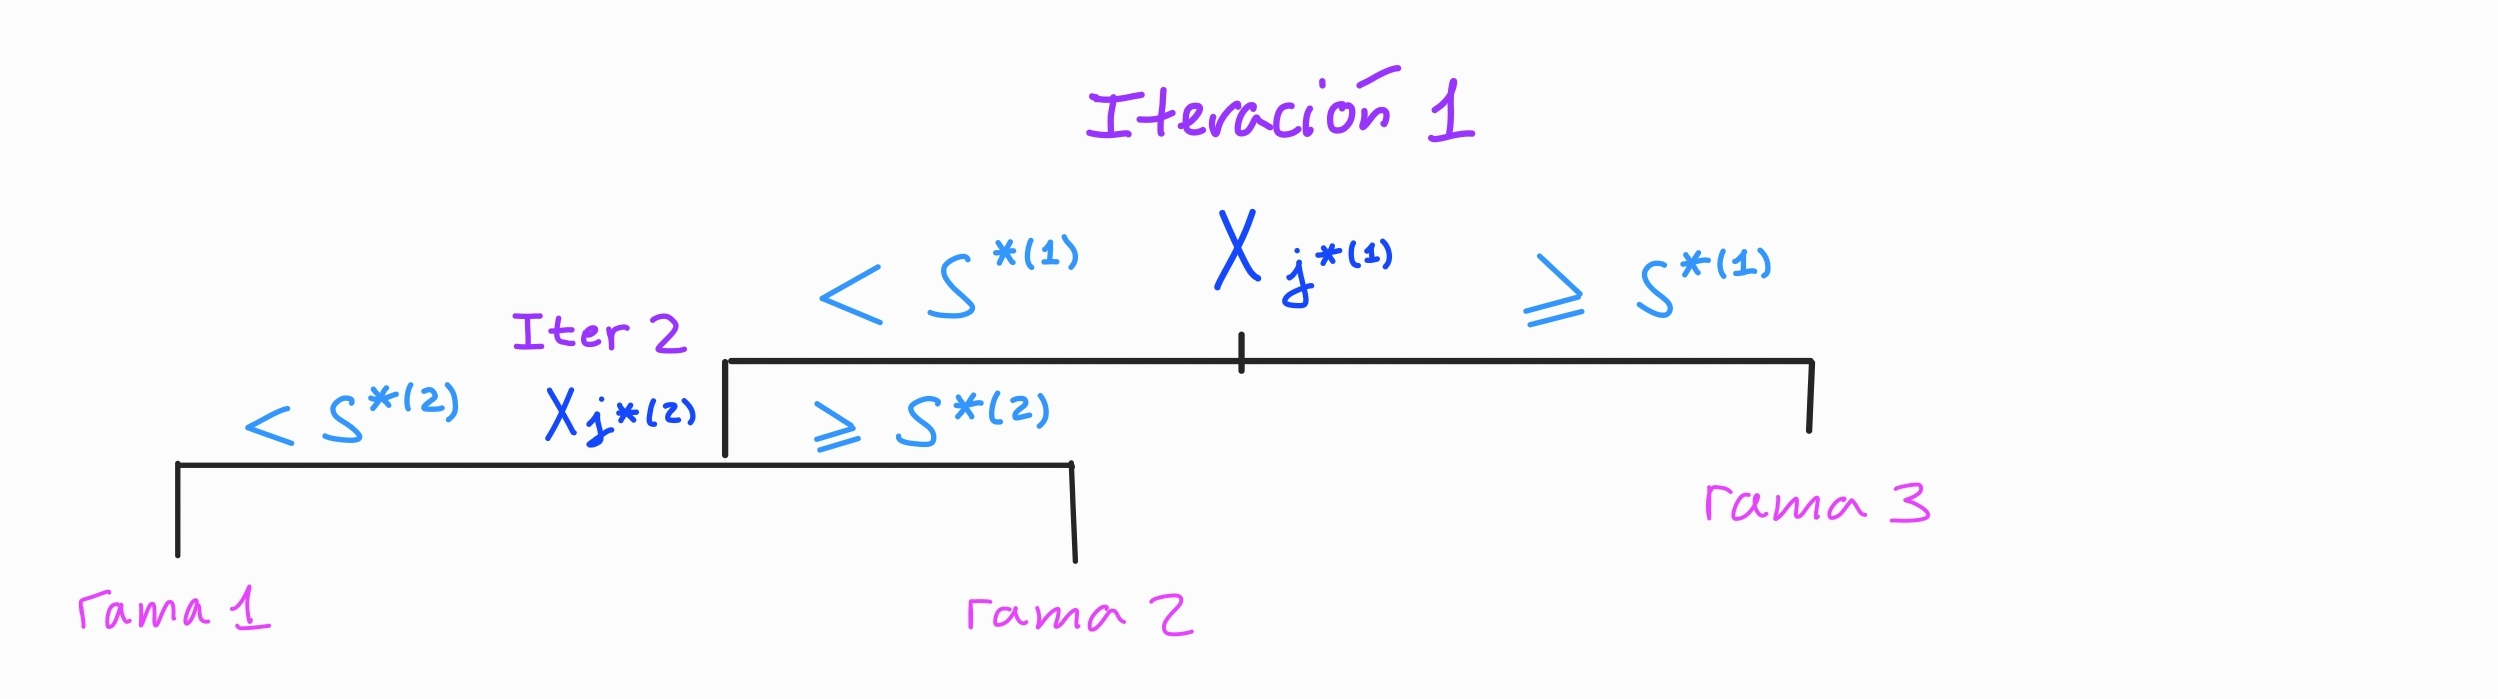
\includegraphics{output_523_0.jpg}
\caption{Arbol óptimo tras resolver el problema de la 2ª Iteración}
\end{figure}

\begin{itemize}
\item
  Si alguna de las ramas tiene menos de
  \(\hspace{0.05cm}k\hspace{0.05cm}\) observaciones de train
  \(\hspace{0.1cm} \Rightarrow \hspace{0.1cm}\) se para el algoritmo
\item
  Si todas las ramas tienen \(\hspace{0.05cm}k\hspace{0.05cm}\) o mas
  observaciones de train \(\hspace{0.1cm} \Rightarrow \hspace{0.1cm}\)
  el algoritmo continua, se pasa a resolver el problema de la iteracion
  siguiente, en este caso el de la iteracion 2
\end{itemize}

\vspace{0.35cm}

\textbf{Problema de la Iteracion 3:}

Arbol con 3 iteraciones tras resolver el problema anterior:

\begin{figure}
\centering
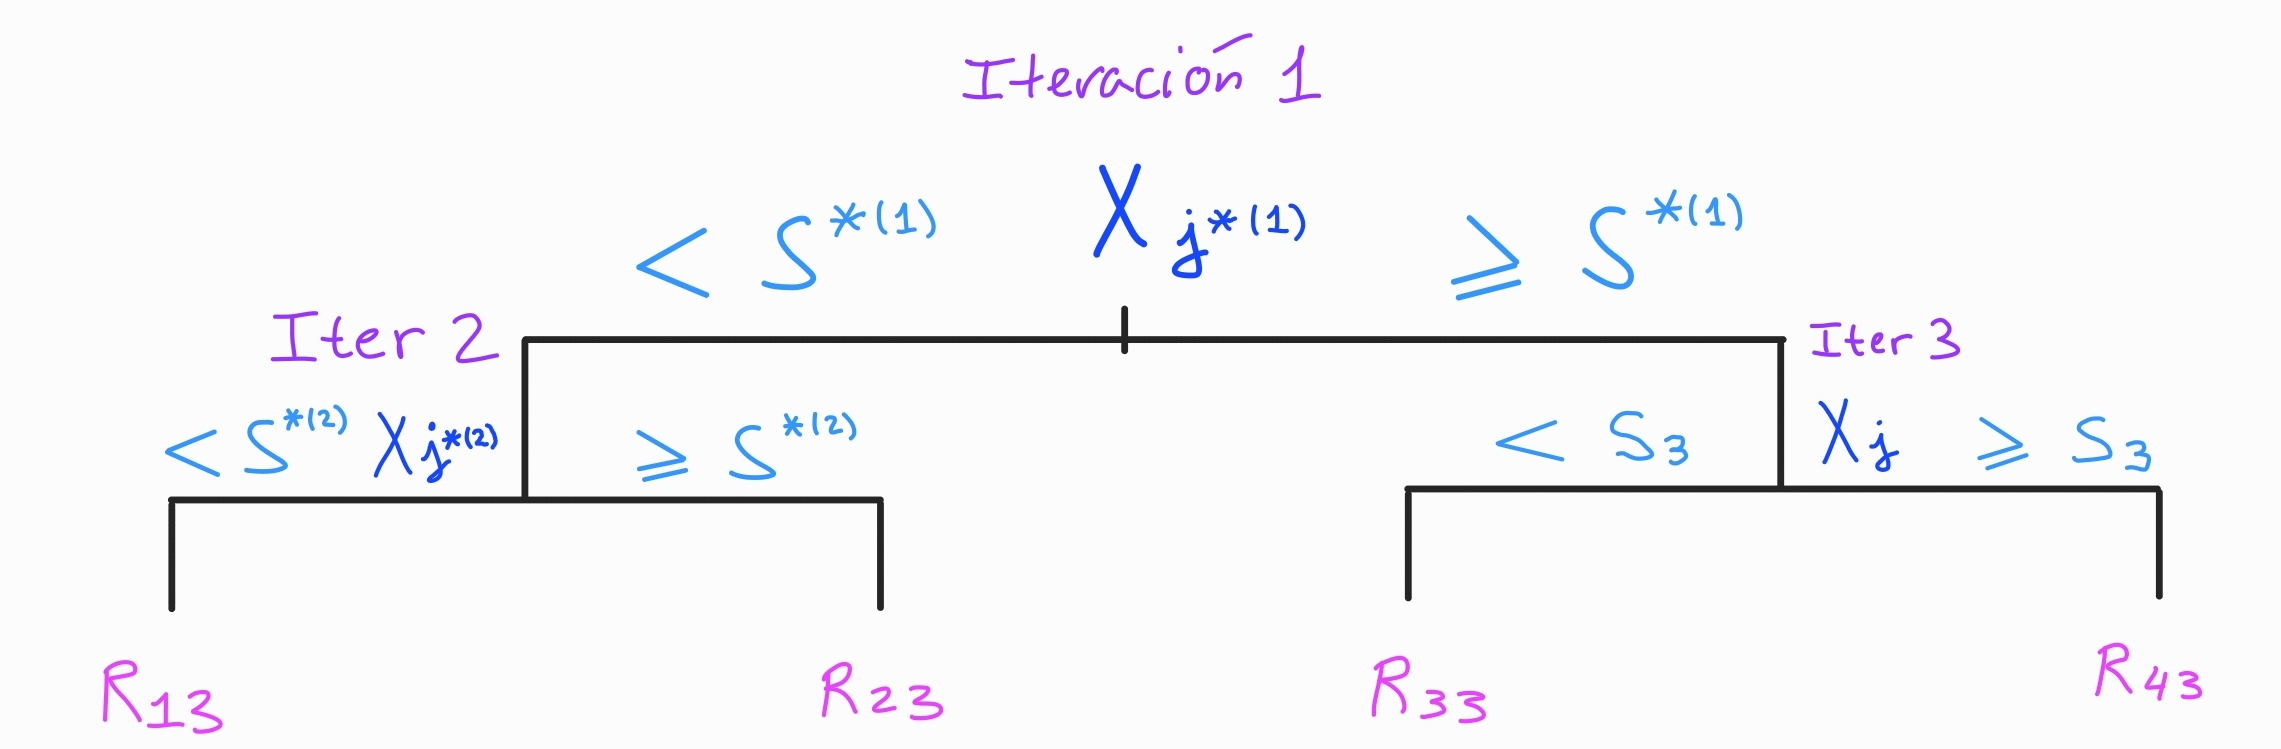
\includegraphics{output_528_0.jpg}
\caption{Arbol con 3 Iteraciones tras resolver el problema de la 2ª
Iteración}
\end{figure}

Si estamos en este problema es porque ninguna rama del arbol resultante
del problema de la Iteracion 2 tiene menos de \(k\) observaciones

La idea es, determinar las regiones \(R_{13}\) , \(R_{23}\), \(R_{33}\)
y \(R_{43}\) del arbol con 3 iteraciones \((\) es decir, \(j\) y
\(s_3 \hspace{0.05cm})\), considerando la solucion del problema de la
iteracion 2 (arbol de arriba), que minimizan el error de entrenamiento
global de dicho arbol.

Notese que \(R_{13}\) y \(R_{23}\) ya están determinadas tras la
resolucion del problema anterior, por ello realmente solo hay que
determinar las regiones \(R_{33}\) y \(R_{43}\) óptimas (a saber, \(j\)
y \(s_3\) óptimos)

\newpage

Mas formalmente el problema se plantea como sigue:

\begin{itemize}
\tightlist
\item
  Usando \(TEC\) como métrica a optimizar
\end{itemize}

\begin{gather*}
\underset{R_{13}  ,  R_{23},  R_{33},  R_{43}}  {Min} \hspace{0.15cm}  \Biggl\{\hspace{0.1cm} TEC_3 = TEC(R_{13})  +  TEC(R_{23}) +  TEC(R_{33}) +  TEC(R_{43}) \hspace{0.1cm} \Biggl\}   \hspace{0.1cm} =   \\ \\
= \underset{R_{13}  ,  R_{23},  R_{33},  R_{43}}  {Min} \hspace{0.1cm}  \Biggl\{ \hspace{0.05cm}   \left( 1 - f_{r^*_{R_{13}} , R_{13}} \right)   \hspace{0.05cm} +  \hspace{0.05cm}    \left( 1 - f_{r^*_{R_{23}} , R_{23}} \right) \hspace{0.05cm} +  \hspace{0.05cm}    \left( 1 - f_{r^*_{R_{33}} , R_{33}} \right)  \hspace{0.05cm} +  \hspace{0.05cm}    \left( 1 - f_{r^*_{R_{43}} , R_{43}} \right)  \hspace{0.05cm}   \Biggl\}  \\ \\    
=\hspace{0.2cm}   \underset{j \hspace{0.02cm},\hspace{0.02cm} s_3}  {Min} \hspace{0.1cm}  \Biggl\{ \hspace{0.2cm}     1 - \dfrac{\# \hspace{0.1 cm}\lbrace i \hspace{0.1 cm}/\hspace{0.1 cm} x_i \in R_{13} \hspace{0.15 cm}\text{y}\hspace{0.15 cm} y_i = r^*_{R_{13}} \rbrace}{\# \hspace{0.1 cm}\lbrace i \hspace{0.1 cm}/\hspace{0.1 cm} x_i \in R_{12}  \rbrace}      \hspace{0.4cm} +  \hspace{0.4cm}   1 - \dfrac{\# \hspace{0.1 cm}\lbrace i \hspace{0.1 cm}/\hspace{0.1 cm} x_i \in R_{23} \hspace{0.15 cm}\text{y}\hspace{0.15 cm} y_i = r^*_{R_{23}} \rbrace}{\# \hspace{0.1 cm}\lbrace i \hspace{0.1 cm}/\hspace{0.1 cm} x_i \in R_{23}  \rbrace} \hspace{0.4cm} +    \hspace{0.4cm}   \\ \\     1 - \dfrac{\# \hspace{0.1 cm}\lbrace i \hspace{0.1 cm}/\hspace{0.1 cm} x_i \in R_{33} \hspace{0.15 cm}\text{y}\hspace{0.15 cm} y_i = r^*_{R_{33}} \rbrace}{\# \hspace{0.1 cm}\lbrace i \hspace{0.1 cm}/\hspace{0.1 cm} x_i \in R_{33}  \rbrace}   \hspace{0.4cm} +    \hspace{0.4cm}       1 - \dfrac{\# \hspace{0.1 cm}\lbrace i \hspace{0.1 cm}/\hspace{0.1 cm} x_i \in R_{43} \hspace{0.15 cm}\text{y}\hspace{0.15 cm} y_i = r^*_{R_{43}} \rbrace}{\# \hspace{0.1 cm}\lbrace i \hspace{0.1 cm}/\hspace{0.1 cm} x_i \in R_{43}  \rbrace} \hspace{0.2cm}    \Biggl\}  \\ \\ 
=\hspace{0.2cm}   \underset{j \hspace{0.02cm},\hspace{0.02cm} s_3}  {Min} \hspace{0.1cm} \Biggl\{ \hspace{0.2cm}     1 - \dfrac{\# \hspace{0.1 cm}\lbrace i \hspace{0.1 cm}/\hspace{0.1 cm}  x_{ij^{*(1)}} \hspace{0.05cm}   < \hspace{0.05cm} s^{*(1)} \hspace{0.25 cm}\text{y}\hspace{0.25 cm} x_{ij^{*(2)}} \hspace{0.05cm}   < \hspace{0.05cm} s^{*(2)} \hspace{0.25 cm}\text{y}\hspace{0.25 cm} y_i = r^*_{R_{13}} \rbrace}{\# \hspace{0.1 cm}\lbrace i \hspace{0.1 cm} / \hspace{0.1 cm}  x_{ij^{*(1)}} \hspace{0.05cm}   < \hspace{0.05cm} s^{*(1)} \hspace{0.25 cm}\text{y}\hspace{0.25 cm} x_{ij} \hspace{0.05cm}   < \hspace{0.05cm} s^{*(2)}  \hspace{0.1 cm} \rbrace }      \hspace{0.4cm} +  \\ \\
\hspace{0.4cm} 1 -  \dfrac{\# \hspace{0.1 cm}\lbrace i \hspace{0.1 cm}/\hspace{0.1 cm}  x_{ij^{*(1)}} \hspace{0.05cm}   < \hspace{0.05cm} s^{*(1)} \hspace{0.25 cm}\text{y}\hspace{0.25 cm} x_{ij} \hspace{0.05cm}   \geqslant \hspace{0.05cm} s^{*(2)} \hspace{0.25 cm}\text{y}\hspace{0.25 cm} y_i = r^*_{R_{23}} \rbrace}{\# \hspace{0.1 cm}\lbrace i \hspace{0.1 cm} / \hspace{0.1 cm}  x_{ij^{*(1)}} \hspace{0.05cm}   < \hspace{0.05cm} s^{*(1)} \hspace{0.25 cm}\text{y}\hspace{0.25 cm} x_{ij} \hspace{0.05cm}   \geqslant \hspace{0.05cm} s^{*(2)}  \hspace{0.1 cm} \rbrace } \hspace{0.3cm} +    \hspace{0.1cm}  \\ \\
1 -  \dfrac{\# \hspace{0.1 cm}\lbrace i \hspace{0.1 cm}/\hspace{0.1 cm}  x_{ij^{*(1)}} \hspace{0.05cm}   \geqslant \hspace{0.05cm} s^{*(1)} \hspace{0.25 cm}\text{y}\hspace{0.25 cm} x_{ij} \hspace{0.05cm}  < \hspace{0.05cm} s_3 \hspace{0.25 cm}\text{y}\hspace{0.25 cm} y_i = r^*_{R_{33}} \rbrace}{\# \hspace{0.1 cm}\lbrace i \hspace{0.1 cm} / \hspace{0.1 cm}  x_{ij^{*(1)}} \hspace{0.05cm}   < \hspace{0.05cm} s^{*(1)} \hspace{0.25 cm}\text{y}\hspace{0.25 cm} x_{ij} \hspace{0.05cm}   < \hspace{0.05cm} s_3  \hspace{0.1 cm} \rbrace }  \hspace{0.2cm}   \hspace{0.3cm} +    \\ \\ 
1 -  \dfrac{\# \hspace{0.1 cm}\lbrace i \hspace{0.1 cm}/\hspace{0.1 cm}  x_{ij^{*(1)}} \hspace{0.05cm}   \geqslant \hspace{0.05cm} s^{*(1)} \hspace{0.25 cm}\text{y}\hspace{0.25 cm} x_{ij} \hspace{0.05cm}  \geqslant \hspace{0.05cm} s_3 \hspace{0.25 cm}\text{y}\hspace{0.25 cm} y_i = r^*_{R_{43}} \rbrace}{\# \hspace{0.1 cm}\lbrace i \hspace{0.1 cm} / \hspace{0.1 cm}  x_{ij^{*(1)}} \hspace{0.05cm}   < \hspace{0.05cm} s^{*(1)} \hspace{0.25 cm}\text{y}\hspace{0.25 cm} x_{ij} \hspace{0.05cm}   \geqslant \hspace{0.05cm} s_3  \hspace{0.1 cm} \rbrace }  \hspace{0.2cm} \Biggl\}
\\ \\  =\hspace{0.2cm}   \underset{j \hspace{0.02cm},\hspace{0.02cm} s_3}  {Min} \hspace{0.1cm} \Biggl\{   \hspace{0.2cm}    1 -   \dfrac{\# \hspace{0.1 cm}\lbrace i \hspace{0.1 cm}/\hspace{0.1 cm}  x_{ij^{*(1)}} \hspace{0.05cm}   \geqslant \hspace{0.05cm} s^{*(1)} \hspace{0.25 cm}\text{y}\hspace{0.25 cm} x_{ij} \hspace{0.05cm}  < \hspace{0.05cm} s_3 \hspace{0.25 cm}\text{y}\hspace{0.25 cm} y_i = r^*_{R_{33}} \rbrace}{\# \hspace{0.1 cm}\lbrace i \hspace{0.1 cm} / \hspace{0.1 cm}  x_{ij^{*(1)}} \hspace{0.05cm}   < \hspace{0.05cm} s^{*(1)} \hspace{0.25 cm}\text{y}\hspace{0.25 cm} x_{ij} \hspace{0.05cm}   < \hspace{0.05cm} s_3  \hspace{0.1 cm} \rbrace }    \hspace{0.3cm} +    \\ \\  \hspace{0.3cm}      1 -  \dfrac{\# \hspace{0.1 cm}\lbrace i \hspace{0.1 cm}/\hspace{0.1 cm}  x_{ij^{*(1)}} \hspace{0.05cm}   \geqslant \hspace{0.05cm} s^{*(1)} \hspace{0.25 cm}\text{y}\hspace{0.25 cm} x_{ij} \hspace{0.05cm}  \geqslant \hspace{0.05cm} s_3 \hspace{0.25 cm}\text{y}\hspace{0.25 cm} y_i = r^*_{R_{43}} \rbrace}{\# \hspace{0.1 cm}\lbrace i \hspace{0.1 cm} / \hspace{0.1 cm}  x_{ij^{*(1)}} \hspace{0.05cm}   < \hspace{0.05cm} s^{*(1)} \hspace{0.25 cm}\text{y}\hspace{0.25 cm} x_{ij} \hspace{0.05cm}   \geqslant \hspace{0.05cm} s_3  \hspace{0.1 cm} \rbrace }  \hspace{0.2cm}      \Biggl\} \\ \\
=\hspace{0.2cm}   \underset{j \hspace{0.02cm},\hspace{0.02cm} s_3}  {Min} \hspace{0.1cm}  \Biggl\{ \hspace{0.2cm}    \left( 1 - f_{r^*_{R_{33}} , R_{33}} \right)  \hspace{0.3cm} +  \hspace{0.1cm}     \left( 1 - f_{r^*_{R_{43}} , R_{43}} \right)   \hspace{0.2cm}  \Biggl\} \\ \\
=\hspace{0.2cm} \underset{  R_{33},  R_{43}}  {Min} \hspace{0.15cm}  \Biggl\{\hspace{0.1cm} TEC(R_{33}) +  TEC(R_{43}) \hspace{0.1cm} \Biggl\}   \hspace{0.1cm} 
\end{gather*}

\newpage

Arbol tras resolver el problema de la Iteración 3:

\begin{figure}
\centering
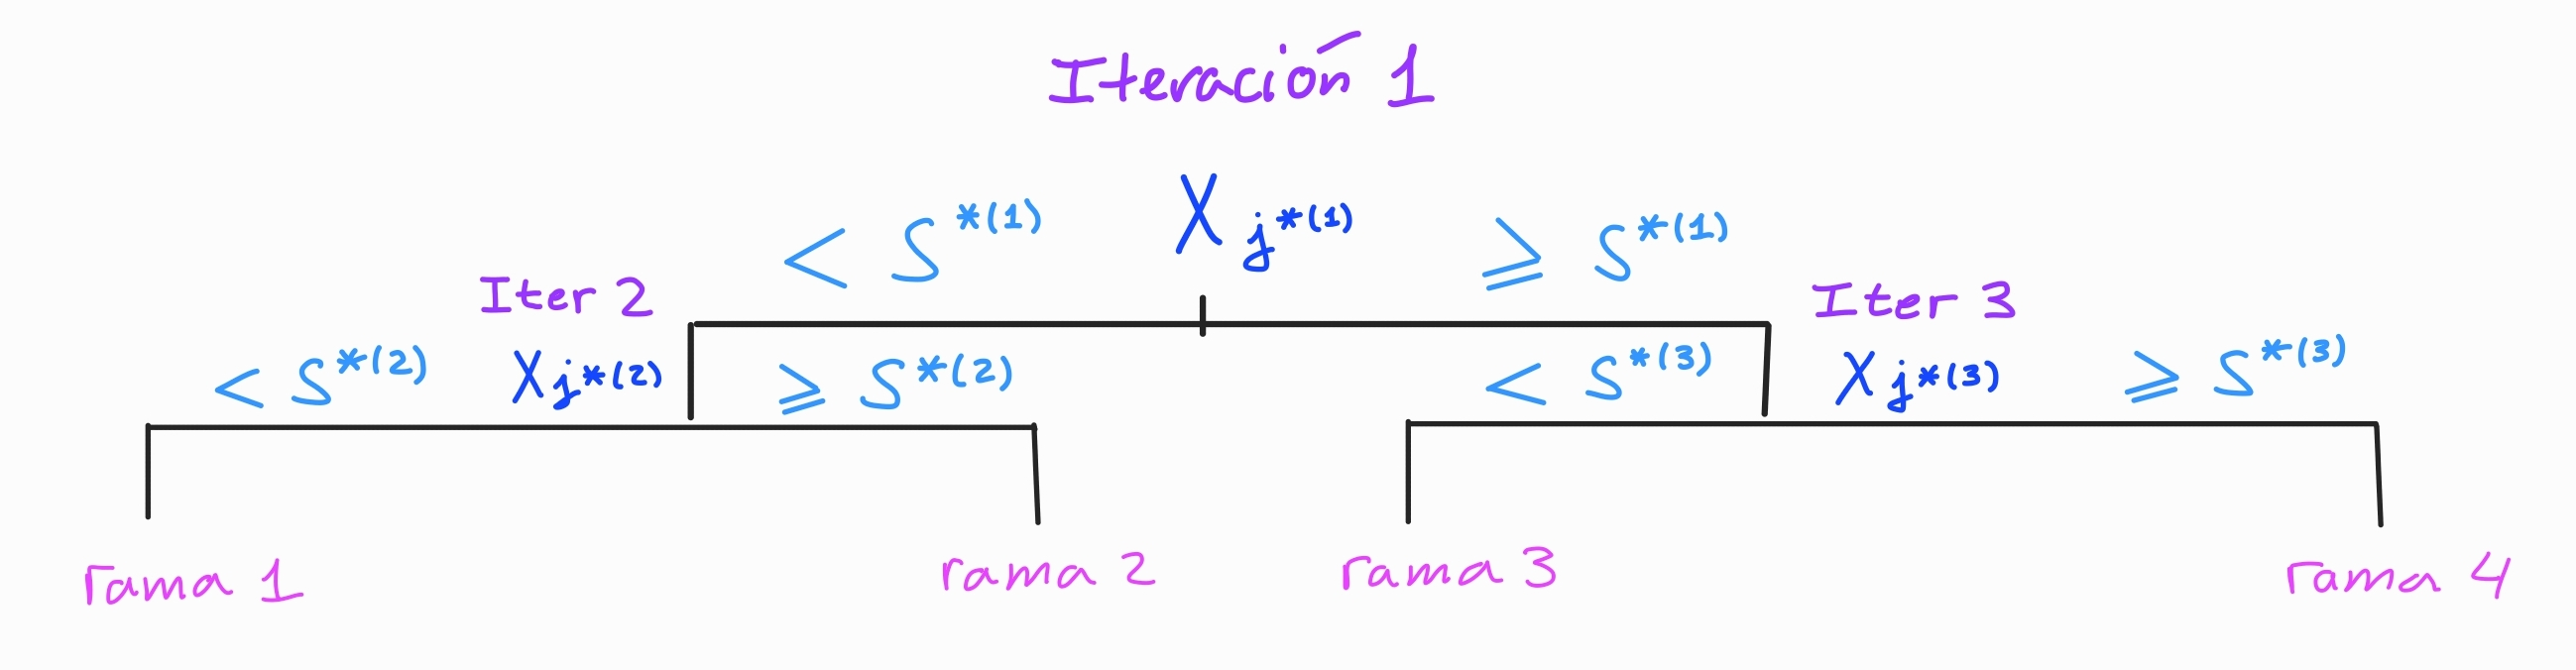
\includegraphics{output_544_0.jpg}
\caption{Arbol tras resolver el problema de la 3ª Iteración}
\end{figure}

\begin{itemize}
\item
  Si alguna de las ramas tiene menos de
  \(\hspace{0.05cm}k\hspace{0.05cm}\) observaciones de train
  \(\hspace{0.1cm} \Rightarrow \hspace{0.1cm}\) se para el algoritmo
\item
  Si todas las ramas tienen \(\hspace{0.05cm}k\hspace{0.05cm}\) o mas
  observaciones de train \(\hspace{0.1cm} \Rightarrow \hspace{0.1cm}\)
  el algoritmo continua, se pasa a resolver el problema de la iteracion
  siguiente, en este caso el de la iteracion 2
\end{itemize}

Siempre que no se cumpla la condicion de parada se seguiria haciendo
crecer el arbol generando nuevas iteraciones.

No seguiremos exponiendo mas iteraciones del algoritmo, puesto que es
facilmente extrapolable lo expuesto a cualquier iteracion superior.

\newpage

\hypertarget{arboles-de-clasificaciuxf3n-penalizados}{%
\subsubsection{Arboles de Clasificación
Penalizados}\label{arboles-de-clasificaciuxf3n-penalizados}}

La idea es esencialmente la misma la ya comentada en la sección de
arboles de regresion penalizados.

Los arboles de clasificación penalizados son esencialemte iguales que
los arboles de clasificacion ordinarios pero tienen una modificacion en
el problema de optimizacion tal que permiten penalizar los arboles con
muchas ramas.

El problema de optimizacion a resolver en los arboles de regresion
ordinarios (usando Gini como métrica, sin perdida de generalidad) era:

\[ \underset{R_1,..,R_m}{Min}  \hspace{0.12cm}  \sum_{h=1}^{m} \hspace{0.1cm} G_{R_{ht}}  \]

En los arboles de regresion penalizados el problema a resolver es:

\[ \underset{R_1,..,R_m}{Min}  \hspace{0.12cm}  \sum_{h=1}^{m} \hspace{0.1cm} G_{R_{ht}} + \alpha \cdot m \]

Donde \(m\) es el numero de ramas del arbol

De este modo, si \(\alpha = 0\) estamos en el caso de arboles de
clasificacion ordinarios.

Si \(\alpha > 0\) , entonces se penalizara el numero de ramas del arbil
(m).

Dado un \(\alpha >0\) , cuanto mayor sea el tamaño del arbol (m) mas
dificil sera que sea optimo en el sentido de que resuelva el probema
deminimizacion. Y viceversa.

Cuanto mayor sea \(\alpha\) más se estará penalizando a los arboles de
tamaño grande.

Con \(\alpha >0\) ( y especialmente \(\alpha >> 0\) ( relativamente
grande)) tienden a salir como optimos arboles que son mas pequeños que
los que salen pusando elalgoritmo ordinario (sin penalizacion).

En el algoritmo ordinario se prioriza que el arbol se ajuste a los datos
de entrenamiento, lo que psuele provocar overfiting (sobreajuse). Esto
es un problema porque hace que el arbol funcione muy bien (prediga bien)
en la muestra de entrenamiento (cuando usa los datos que ya ha
``visto''), pero bastante peor en la muestra de test. Estos modelos
tendran poco sesgo pero mucha varianza a nivel predictivo, lo cual es
negativo.

El algoritmo penalizado permite obtener un equilibrio entre sesgo y
varianza a traves del parametro de penalizacion \(\alpha\)

La idea es seleccionar un alpha que nos genere un modelo con quiza un
poco mas de sesgo pero con considerable menos varianza que el ordinario,
lo cualq conduzca a un erro de prediccion menor que en el caso
ordinario.

\vspace{0.15cm}

\textbf{¿ Cómo escoger \(\alpha\) en la practica ?}

Una idea razonable es entrenar un arbol con los mismos datos de
entrenamiento pero con \(B\) distintos \(\alpha\)

Calcular con una muestra de test el error de cada uno de los \(B\)
modelos.

Quedarse con el \(\alpha\) asociado al modelo con menor error de test.

Una cuestion relevante aqui es como definir el conjunto de \(B\) valores
de \(\alpha\) que se van a tener en consideracion.

No entraremos aqui en esta cuestión.

\newpage

\hypertarget{arboles-de-clasificaciuxf3n-algoritmo-de-creaciuxf3n-propia-en-python}{%
\subsubsection{\texorpdfstring{Arboles de clasificación: algoritmo de
creación propia en
\texttt{Python}}{Arboles de clasificación: algoritmo de creación propia en Python}}\label{arboles-de-clasificaciuxf3n-algoritmo-de-creaciuxf3n-propia-en-python}}

\textbf{Algoritmo de creacion propia con TEC}

\begin{Shaded}
\begin{Highlighting}[]
\KeywordTok{def}\NormalTok{ classification\_tree(Data\_set, iterations\_vector, k, Y\_categories) :}

\CommentTok{\# POR AHORA SOLO GENERA 4 ITERACIONES EN EL ARBOL {-}{-}\textgreater{} iterations\_vector = range(1,5) como mucho (=[1,2,3,4])}

\CommentTok{\# Data\_set tiene que ser tal que, su columna 0 sea Y, y la j{-}esima sea la variable Xj , para j=1,...,p}

\CommentTok{\# Si se quiere que el arbol tenga como mucho 3 iteraciones {-}{-}\textgreater{} iterations\_vector = range(1,4) = [1,2,3]}

\CommentTok{\# Si Y tiene como categorias 0,1,2 {-}{-}\textgreater{} Y\_categories = range(0,3)}

\CommentTok{\# k = numero de obsrevaciones minimas por rama del arbol {-}{-}\textgreater{} criterio de parada}

\CommentTok{\#\#\#\#\#\#\#\#\#\#\#\#\#\#\#\#\#\#\#\#\#\#\#\#\#\#\#\#\#\#\#\#\#\#\#\#\#\#\#\#\#\#\#\#\#\#\#\#\#\#\#\#\#\#\#\#\#\#\#\#\#\#\#\#\#\#\#\#\#\#\#\#}
    
    \KeywordTok{def}\NormalTok{ s\_values(j, Data\_set):}

\NormalTok{        s\_values }\OperatorTok{=}\NormalTok{ []}

        \ControlFlowTok{if}\NormalTok{  (Data\_set.dtypes[j] }\OperatorTok{!=} \StringTok{\textquotesingle{}float64\textquotesingle{}}\NormalTok{) }\OperatorTok{\&}\NormalTok{ (Data\_set.dtypes[j] }\OperatorTok{!=} \StringTok{\textquotesingle{}int64\textquotesingle{}}\NormalTok{) : }\CommentTok{\# Para las variables categoricas s\_value sera simplemente su rango.}

\NormalTok{            s\_values }\OperatorTok{=}\NormalTok{ Data\_set.sort\_values(by}\OperatorTok{=}\NormalTok{[Data\_set.columns[j]], axis}\OperatorTok{=}\DecValTok{0}\NormalTok{, ascending}\OperatorTok{=}\VariableTok{True}\NormalTok{, ignore\_index}\OperatorTok{=}\VariableTok{True}\NormalTok{).iloc[:, j].unique()}


        \ControlFlowTok{elif}\NormalTok{ (Data\_set.dtypes[j] }\OperatorTok{==} \StringTok{\textquotesingle{}float64\textquotesingle{}}\NormalTok{) }\OperatorTok{|}\NormalTok{ (Data\_set.dtypes[j] }\OperatorTok{==} \StringTok{\textquotesingle{}int64\textquotesingle{}}\NormalTok{) :}

\NormalTok{            Xj\_sorted }\OperatorTok{=}\NormalTok{ Data\_set.sort\_values(by}\OperatorTok{=}\NormalTok{[Data\_set.columns[j]], axis}\OperatorTok{=}\DecValTok{0}\NormalTok{, ascending}\OperatorTok{=}\VariableTok{True}\NormalTok{, ignore\_index}\OperatorTok{=}\VariableTok{True}\NormalTok{).iloc[:, j].unique()}

        
            \ControlFlowTok{for}\NormalTok{ i }\KeywordTok{in} \BuiltInTok{range}\NormalTok{(}\DecValTok{0}\NormalTok{, }\BuiltInTok{len}\NormalTok{(Xj\_sorted)}\OperatorTok{{-}}\DecValTok{1}\NormalTok{):}

\NormalTok{                s\_values.append( (Xj\_sorted[i] }\OperatorTok{+}\NormalTok{ Xj\_sorted[i}\OperatorTok{+}\DecValTok{1}\NormalTok{] ) }\OperatorTok{/} \DecValTok{2}\NormalTok{  )}

    
        \ControlFlowTok{return}\NormalTok{ s\_values}


\CommentTok{\#\#\#\#\#\#\#\#\#\#\#\#\#\#\#\#\#\#\#\#\#\#\#\#\#\#\#\#\#\#\#\#\#\#\#\#\#\#\#\#\#\#\#\#\#\#\#\#\#\#\#\#\#\#\#\#\#\#\#\#\#\#\#\#\#\#\#\#\#\#\#\#  }

   \CommentTok{\#\# ITERACION 1}

    \ControlFlowTok{if}\NormalTok{ iterations\_vector[}\DecValTok{0}\NormalTok{] }\OperatorTok{==} \DecValTok{1}\NormalTok{ : }\CommentTok{\# nacimiento del arbol}

        
        \CommentTok{\#\#\#\#\#\#\#\#\#\#\#\#\#\#\#\#\#\#\#\#\#\#\#\#\#\#\#\#\#\#\#\#\#\#\#}
        
        \KeywordTok{def}\NormalTok{ f\_R11(j, s, r, Data\_set):}

           \CommentTok{\# Verificando si se cumplen las siguientes dos condiciones conjuntamente nos garantizamos que todas las ramas tienes observaciones de train. }
           \CommentTok{\# Es decir, no habra ninguna rama sin observaciones de train que caigan en ella.}

\NormalTok{            cond\_R11 }\OperatorTok{=} \BuiltInTok{len}\NormalTok{(Data\_set.loc[ (Data\_set.iloc[:, j] }\OperatorTok{\textless{}}\NormalTok{ s) , : ] )}

            \ControlFlowTok{if}\NormalTok{  cond\_R11 }\OperatorTok{!=} \DecValTok{0}\NormalTok{ :}

\NormalTok{                f\_R11 }\OperatorTok{=} \BuiltInTok{len}\NormalTok{( Data\_set.loc[ (Data\_set.iloc[:, j] }\OperatorTok{\textless{}}\NormalTok{ s) }\OperatorTok{\&}\NormalTok{ (Data\_set.loc[:, }\StringTok{\textquotesingle{}Y\textquotesingle{}}\NormalTok{] }\OperatorTok{==}\NormalTok{ r) , : ] ) }\OperatorTok{/} \BuiltInTok{len}\NormalTok{( Data\_set.loc[ (Data\_set.iloc[:, j] }\OperatorTok{\textless{}}\NormalTok{ s) , : ] )}

            
            \ControlFlowTok{elif}\NormalTok{ cond\_R11 }\OperatorTok{==} \DecValTok{0}\NormalTok{ :}

\NormalTok{                f\_R11 }\OperatorTok{=} \DecValTok{0}

            
            \ControlFlowTok{return}\NormalTok{ f\_R11 }

        \CommentTok{\#\#\#\#\#\#\#\#\#\#\#\#\#\#\#\#\#\#\#\#\#\#\#\#\#\#\#\#\#\#\#\#\#\#\#\#\#\#}

        \KeywordTok{def}\NormalTok{ f\_R21(j, s, r, Data\_set):}

\NormalTok{            cond\_R21 }\OperatorTok{=} \BuiltInTok{len}\NormalTok{(Data\_set.loc[ (Data\_set.iloc[:, j] }\OperatorTok{\textgreater{}=}\NormalTok{ s) , : ] )}

            \ControlFlowTok{if}\NormalTok{ cond\_R21 }\OperatorTok{!=} \DecValTok{0}\NormalTok{ :}

\NormalTok{                f\_R21 }\OperatorTok{=} \BuiltInTok{len}\NormalTok{( Data\_set.loc[ (Data\_set.iloc[:, j] }\OperatorTok{\textgreater{}=}\NormalTok{ s) }\OperatorTok{\&}\NormalTok{ (Data\_set.loc[:, }\StringTok{\textquotesingle{}Y\textquotesingle{}}\NormalTok{] }\OperatorTok{==}\NormalTok{ r) , : ] ) }\OperatorTok{/} \BuiltInTok{len}\NormalTok{( Data\_set.loc[ (Data\_set.iloc[:, j] }\OperatorTok{\textgreater{}=}\NormalTok{ s) , : ] )}
            
            \ControlFlowTok{elif}\NormalTok{ cond\_R21 }\OperatorTok{==} \DecValTok{0}\NormalTok{ :}

\NormalTok{                f\_R21 }\OperatorTok{=} \DecValTok{0}

            
            \ControlFlowTok{return}\NormalTok{ f\_R21 }


        \CommentTok{\#\#\#\#\#\#\#\#\#\#\#\#\#\#\#\#\#\#\#\#\#\#\#\#\#\#\#\#\#\#\#\#\#\#\#}

\NormalTok{        TEC\_vector }\OperatorTok{=}\NormalTok{ []}
\NormalTok{        j\_vector }\OperatorTok{=}\NormalTok{ []}
\NormalTok{        s\_vector }\OperatorTok{=}\NormalTok{ []}

\NormalTok{        j\_star\_vector }\OperatorTok{=}\NormalTok{ []}
\NormalTok{        s\_star\_vector }\OperatorTok{=}\NormalTok{ []}
\NormalTok{        TEC\_star\_vector }\OperatorTok{=}\NormalTok{ []}

        \ControlFlowTok{for}\NormalTok{ j }\KeywordTok{in} \BuiltInTok{range}\NormalTok{(}\DecValTok{1}\NormalTok{, Data\_set.shape[}\DecValTok{1}\NormalTok{]) :}

            \ControlFlowTok{for}\NormalTok{ s }\KeywordTok{in}\NormalTok{ s\_values(j, Data\_set) :}

                \CommentTok{\# Busqueda de r\_star\_R11 :}

\NormalTok{                f\_R11\_r\_vector }\OperatorTok{=}\NormalTok{ []}

                \ControlFlowTok{for}\NormalTok{ r }\KeywordTok{in}\NormalTok{ Y\_categories:  }\CommentTok{\# Si Y tiene como categorias 0,1,2 {-}{-}\textgreater{} Y\_categories = range(0,3)}

\NormalTok{                    f\_R11\_r\_vector.append( f\_R11(j, s, r , Data\_set) )}

\NormalTok{                f\_R11\_df }\OperatorTok{=}\NormalTok{ pd.DataFrame(\{}\StringTok{\textquotesingle{}r\textquotesingle{}}\NormalTok{:Y\_categories  , }\StringTok{\textquotesingle{}f\_R11\textquotesingle{}}\NormalTok{:f\_R11\_r\_vector \})}
        
\NormalTok{                f\_R11\_df\_sorted }\OperatorTok{=}\NormalTok{ f\_R11\_df.sort\_values(by}\OperatorTok{=}\NormalTok{[}\StringTok{\textquotesingle{}f\_R11\textquotesingle{}}\NormalTok{], axis}\OperatorTok{=}\DecValTok{0}\NormalTok{, ascending}\OperatorTok{=}\VariableTok{False}\NormalTok{, ignore\_index}\OperatorTok{=}\VariableTok{True}\NormalTok{)}

\NormalTok{                r\_star\_R11 }\OperatorTok{=}\NormalTok{ f\_R11\_df\_sorted.loc[}\DecValTok{0}\NormalTok{, }\StringTok{\textquotesingle{}r\textquotesingle{}}\NormalTok{]}


                \CommentTok{\# Busqueda de r\_star\_R21 :}

\NormalTok{                f\_R21\_r\_vector }\OperatorTok{=}\NormalTok{ []}

                \ControlFlowTok{for}\NormalTok{ r }\KeywordTok{in}\NormalTok{ Y\_categories:  }\CommentTok{\# Si Y tiene como categorias 0,1,2 {-}{-}\textgreater{} Y\_categories = range(0,3)}

\NormalTok{                    f\_R21\_r\_vector.append( f\_R21(j, s, r , Data\_set) )}

\NormalTok{                f\_R21\_df }\OperatorTok{=}\NormalTok{ pd.DataFrame(\{}\StringTok{\textquotesingle{}r\textquotesingle{}}\NormalTok{:Y\_categories  , }\StringTok{\textquotesingle{}f\_R21\textquotesingle{}}\NormalTok{:f\_R21\_r\_vector \})}
        
\NormalTok{                f\_R21\_df\_sorted }\OperatorTok{=}\NormalTok{ f\_R21\_df.sort\_values(by}\OperatorTok{=}\NormalTok{[}\StringTok{\textquotesingle{}f\_R21\textquotesingle{}}\NormalTok{], axis}\OperatorTok{=}\DecValTok{0}\NormalTok{, ascending}\OperatorTok{=}\VariableTok{False}\NormalTok{, ignore\_index}\OperatorTok{=}\VariableTok{True}\NormalTok{)}

\NormalTok{                r\_star\_R21 }\OperatorTok{=}\NormalTok{ f\_R21\_df\_sorted.loc[}\DecValTok{0}\NormalTok{, }\StringTok{\textquotesingle{}r\textquotesingle{}}\NormalTok{]}


                \CommentTok{\# Calculo de TEC\_1 para la combinacion (j, s) dada:}

\NormalTok{                TEC\_1 }\OperatorTok{=} \DecValTok{1}\OperatorTok{{-}}\NormalTok{ f\_R11(j, s, r\_star\_R11, Data\_set) }\OperatorTok{+} \DecValTok{1}\OperatorTok{{-}}\NormalTok{ f\_R21(j, s, r\_star\_R21, Data\_set)}

\NormalTok{                TEC\_vector.append(TEC\_1)}
\NormalTok{                j\_vector.append(j)}
\NormalTok{                s\_vector.append(s)}


        \CommentTok{\# Busqueda de j\_star y s\_star de la itracion 1:}

\NormalTok{        TEC\_df }\OperatorTok{=}\NormalTok{ pd.DataFrame(\{}\StringTok{\textquotesingle{}TEC\textquotesingle{}}\NormalTok{:TEC\_vector, }\StringTok{\textquotesingle{}j\textquotesingle{}}\NormalTok{:j\_vector, }\StringTok{\textquotesingle{}s\textquotesingle{}}\NormalTok{:s\_vector\})}

\NormalTok{        TEC\_df\_sorted }\OperatorTok{=}\NormalTok{ TEC\_df.sort\_values(by}\OperatorTok{=}\NormalTok{[}\StringTok{\textquotesingle{}TEC\textquotesingle{}}\NormalTok{], axis}\OperatorTok{=}\DecValTok{0}\NormalTok{, ascending}\OperatorTok{=}\VariableTok{True}\NormalTok{, ignore\_index}\OperatorTok{=}\VariableTok{True}\NormalTok{)}

\NormalTok{        s\_star\_vector.append( TEC\_df\_sorted.loc[}\DecValTok{0}\NormalTok{, }\StringTok{\textquotesingle{}s\textquotesingle{}}\NormalTok{] )}
\NormalTok{        j\_star\_vector.append( TEC\_df\_sorted.loc[}\DecValTok{0}\NormalTok{, }\StringTok{\textquotesingle{}j\textquotesingle{}}\NormalTok{] )}
\NormalTok{        TEC\_star\_vector.append(TEC\_df\_sorted.loc[}\DecValTok{0}\NormalTok{, }\StringTok{\textquotesingle{}TEC\textquotesingle{}}\NormalTok{])}

        \CommentTok{\# OJO: s\_star\_vector[i] sera el s\_star de la iteracion i+1 , para i=0,1,...}
        \CommentTok{\# OJO: j\_star\_vector[i] sera el j\_star de la iteracion i+1 , para i=0,1,...    }
        
      \CommentTok{\#\#\#\#\#\#\#\#\#\#\#\#\#\#\#\#\#\#\#\#\#\#\#\#\#\#\#\#\#\#\#\#\#\#\#}

        \CommentTok{\# Condicion de parada:}

\NormalTok{        obs\_r11 }\OperatorTok{=} \BuiltInTok{len}\NormalTok{( Data\_set.loc[ Data\_set.iloc[:, j\_star\_vector[}\DecValTok{0}\NormalTok{] ] }\OperatorTok{\textless{}}\NormalTok{ s\_star\_vector[}\DecValTok{0}\NormalTok{] , : ] )}
\NormalTok{        obs\_r21 }\OperatorTok{=} \BuiltInTok{len}\NormalTok{( Data\_set.loc[ Data\_set.iloc[:, j\_star\_vector[}\DecValTok{0}\NormalTok{] ] }\OperatorTok{\textgreater{}=}\NormalTok{ s\_star\_vector[}\DecValTok{0}\NormalTok{] , : ] )}

        \ControlFlowTok{if}\NormalTok{(obs\_r11 }\OperatorTok{\textless{}}\NormalTok{ k) }\OperatorTok{|}\NormalTok{ (obs\_r21 }\OperatorTok{\textless{}}\NormalTok{ k) : }\CommentTok{\# Si se cumple el criterio de parada}


            \BuiltInTok{print}\NormalTok{(}\StringTok{\textquotesingle{}El arbol final es el arbol con 1 Iteracion. Se ha cumplido el criterio de parada basado en numero minimo\textquotesingle{}}\NormalTok{, k ,}\StringTok{\textquotesingle{}de observaciones por rama\textquotesingle{}}\NormalTok{)}

\NormalTok{            number\_iterations}\OperatorTok{=}\DecValTok{1}

\NormalTok{            obs\_ramas }\OperatorTok{=}\NormalTok{ [obs\_r11 , obs\_r21]}

       
            \CommentTok{\#\#\#\#\#\#\#\#\#\#\#\#\#\#\#\#\#\#\#}
            
            \ControlFlowTok{return}\NormalTok{(number\_iterations, j\_star\_vector, s\_star\_vector, TEC\_star\_vector, obs\_ramas ) }

            \CommentTok{\#\#\#\#\#\#\#\#\#\#\#\#\#\#\#\#\#\#\#}

        \ControlFlowTok{elif}\NormalTok{ (obs\_r11 }\OperatorTok{\textgreater{}=}\NormalTok{ k) }\OperatorTok{\&}\NormalTok{ (obs\_r21 }\OperatorTok{\textgreater{}=}\NormalTok{ k) : }\CommentTok{\# No se cumple el criterio de parada}

            \ControlFlowTok{pass}


\CommentTok{\#\#\#\#\#\#\#\#\#\#\#\#\#\#\#\#\#\#\#\#\#\#\#\#\#\#\#\#\#\#\#\#\#\#\#\#\#\#\#\#\#\#\#\#\#\#\#\#\#\#\#\#\#\#\#\#\#\#\#\#\#\#\#\#\#\#\#\#\#\#\#}

    \CommentTok{\#\# ITERACION 2   ·········· POR MODIFICAR !! ·············}

    \ControlFlowTok{if}\NormalTok{ iterations\_vector[}\DecValTok{1}\NormalTok{] }\OperatorTok{==} \DecValTok{2}\NormalTok{ :  }\CommentTok{\# Desarrollar nodo R1 de la 1ª iteracion}

    \CommentTok{\#\#\#\#\#\#\#\#\#\#\#\#\#\#\#\#\#\#\#\#\#\#\#\#\#\#\#\#\#\#\#\#\#\#\#\#\#\#\#\#\#\#\#\#\#\#\#\#\#\#\#\#\#\#\#\#\#\#\#\#\#\#\#\#}


        \KeywordTok{def}\NormalTok{ f\_R12(j, s, r, Data\_set):}

           \CommentTok{\# Verificando si se cumplen las siguientes dos condiciones conjuntamente nos garantizamos que todas las ramas tienes observaciones de train. }
           \CommentTok{\# Es decir, no habra ninguna rama sin observaciones de train que caigan en ella.}

\NormalTok{            cond\_R12 }\OperatorTok{=} \BuiltInTok{len}\NormalTok{( Data\_set.loc[ (Data\_set.iloc[:, j\_star\_vector[}\DecValTok{0}\NormalTok{]] }\OperatorTok{\textless{}}\NormalTok{ s\_star\_vector[}\DecValTok{0}\NormalTok{]) }\OperatorTok{\&}\NormalTok{ (Data\_set.iloc[:, j] }\OperatorTok{\textless{}}\NormalTok{ s) , : ] ) }

            \ControlFlowTok{if}\NormalTok{  cond\_R12 }\OperatorTok{!=} \DecValTok{0}\NormalTok{ :}

\NormalTok{                f\_R12 }\OperatorTok{=} \BuiltInTok{len}\NormalTok{( Data\_set.loc[ (Data\_set.iloc[:, j\_star\_vector[}\DecValTok{0}\NormalTok{]] }\OperatorTok{\textless{}}\NormalTok{ s\_star\_vector[}\DecValTok{0}\NormalTok{]) }\OperatorTok{\&}\NormalTok{ (Data\_set.iloc[:, j] }\OperatorTok{\textless{}}\NormalTok{ s) }\OperatorTok{\&}\NormalTok{ (Data\_set.loc[:, }\StringTok{\textquotesingle{}Y\textquotesingle{}}\NormalTok{] }\OperatorTok{==}\NormalTok{ r) , : ] ) }\OperatorTok{/}\NormalTok{ cond\_R12}

            
            \ControlFlowTok{elif}\NormalTok{ cond\_R12 }\OperatorTok{==} \DecValTok{0}\NormalTok{ :}

\NormalTok{                f\_R12 }\OperatorTok{=} \DecValTok{0}

            
            \ControlFlowTok{return}\NormalTok{ f\_R12 }

        \CommentTok{\#\#\#\#\#\#\#\#\#}

        \KeywordTok{def}\NormalTok{ f\_R22(j, s, r, Data\_set):}

           \CommentTok{\# Verificando si se cumplen las siguientes dos condiciones conjuntamente nos garantizamos que todas las ramas tienes observaciones de train. }
           \CommentTok{\# Es decir, no habra ninguna rama sin observaciones de train que caigan en ella.}

\NormalTok{            cond\_R22 }\OperatorTok{=} \BuiltInTok{len}\NormalTok{( Data\_set.loc[ (Data\_set.iloc[:, j\_star\_vector[}\DecValTok{0}\NormalTok{]] }\OperatorTok{\textless{}}\NormalTok{ s\_star\_vector[}\DecValTok{0}\NormalTok{]) }\OperatorTok{\&}\NormalTok{ (Data\_set.iloc[:, j] }\OperatorTok{\textgreater{}=}\NormalTok{ s) , : ] ) }

            \ControlFlowTok{if}\NormalTok{  cond\_R22 }\OperatorTok{!=} \DecValTok{0}\NormalTok{ :}

\NormalTok{                f\_R22 }\OperatorTok{=} \BuiltInTok{len}\NormalTok{( Data\_set.loc[ (Data\_set.iloc[:, j\_star\_vector[}\DecValTok{0}\NormalTok{]] }\OperatorTok{\textless{}}\NormalTok{ s\_star\_vector[}\DecValTok{0}\NormalTok{]) }\OperatorTok{\&}\NormalTok{ (Data\_set.iloc[:, j] }\OperatorTok{\textgreater{}=}\NormalTok{ s) }\OperatorTok{\&}\NormalTok{ (Data\_set.loc[:, }\StringTok{\textquotesingle{}Y\textquotesingle{}}\NormalTok{] }\OperatorTok{==}\NormalTok{ r) , : ] ) }\OperatorTok{/}\NormalTok{ cond\_R22}

            
            \ControlFlowTok{elif}\NormalTok{ cond\_R22 }\OperatorTok{==} \DecValTok{0}\NormalTok{ :}

\NormalTok{                f\_R22 }\OperatorTok{=} \DecValTok{0}

            
            \ControlFlowTok{return}\NormalTok{ f\_R22 }


        \CommentTok{\#\#\#\#\#\#\#\#\#\#\#\#\#\#\#\#\#\#\#\#\#\#\#\#\#\#\#\#\#\#\#\#\#\#\#}

\NormalTok{        TEC\_vector }\OperatorTok{=}\NormalTok{ []}
\NormalTok{        j\_vector }\OperatorTok{=}\NormalTok{ []}
\NormalTok{        s\_vector }\OperatorTok{=}\NormalTok{ []}


        \ControlFlowTok{for}\NormalTok{ j }\KeywordTok{in} \BuiltInTok{range}\NormalTok{(}\DecValTok{1}\NormalTok{, Data\_set.shape[}\DecValTok{1}\NormalTok{]) :}

            \ControlFlowTok{for}\NormalTok{ s }\KeywordTok{in}\NormalTok{ s\_values(j, Data\_set) :}

                \CommentTok{\# Busqueda de r\_star\_R12 :}

\NormalTok{                f\_R12\_r\_vector }\OperatorTok{=}\NormalTok{ []}

                \ControlFlowTok{for}\NormalTok{ r }\KeywordTok{in}\NormalTok{ Y\_categories :  }\CommentTok{\# Si Y tiene como categorias 0,1,2 {-}{-}\textgreater{} Y\_categories = range(0,3)}

\NormalTok{                    f\_R12\_r\_vector.append( f\_R12(j, s, r , Data\_set) )}

\NormalTok{                f\_R12\_df }\OperatorTok{=}\NormalTok{ pd.DataFrame(\{}\StringTok{\textquotesingle{}r\textquotesingle{}}\NormalTok{:Y\_categories  , }\StringTok{\textquotesingle{}f\_R12\textquotesingle{}}\NormalTok{:f\_R11\_r\_vector \})}
        
\NormalTok{                f\_R12\_df\_sorted }\OperatorTok{=}\NormalTok{ f\_R12\_df.sort\_values(by}\OperatorTok{=}\NormalTok{[}\StringTok{\textquotesingle{}f\_R12\textquotesingle{}}\NormalTok{], axis}\OperatorTok{=}\DecValTok{0}\NormalTok{, ascending}\OperatorTok{=}\VariableTok{False}\NormalTok{, ignore\_index}\OperatorTok{=}\VariableTok{True}\NormalTok{)}

\NormalTok{                r\_star\_R12 }\OperatorTok{=}\NormalTok{ f\_R11\_df\_sorted.loc[}\DecValTok{0}\NormalTok{, }\StringTok{\textquotesingle{}r\textquotesingle{}}\NormalTok{]}


                \CommentTok{\# Busqueda de r\_star\_R22 :}

\NormalTok{                f\_R22\_r\_vector }\OperatorTok{=}\NormalTok{ []}

                \ControlFlowTok{for}\NormalTok{ r }\KeywordTok{in}\NormalTok{ Y\_categories:  }\CommentTok{\# Si Y tiene como categorias 0,1,2 {-}{-}\textgreater{} Y\_categories = range(0,3)}

\NormalTok{                    f\_R22\_r\_vector.append( f\_R22(j, s, r , Data\_set) )}

\NormalTok{                f\_R22\_df }\OperatorTok{=}\NormalTok{ pd.DataFrame(\{}\StringTok{\textquotesingle{}r\textquotesingle{}}\NormalTok{:Y\_categories , }\StringTok{\textquotesingle{}f\_R22\textquotesingle{}}\NormalTok{:f\_R22\_r\_vector \})}
        
\NormalTok{                f\_R22\_df\_sorted }\OperatorTok{=}\NormalTok{ f\_R22\_df.sort\_values(by}\OperatorTok{=}\NormalTok{[}\StringTok{\textquotesingle{}f\_R22\textquotesingle{}}\NormalTok{], axis}\OperatorTok{=}\DecValTok{0}\NormalTok{, ascending}\OperatorTok{=}\VariableTok{False}\NormalTok{, ignore\_index}\OperatorTok{=}\VariableTok{True}\NormalTok{)}

\NormalTok{                r\_star\_R22 }\OperatorTok{=}\NormalTok{ f\_R22\_df\_sorted.loc[}\DecValTok{0}\NormalTok{, }\StringTok{\textquotesingle{}r\textquotesingle{}}\NormalTok{]}


                \CommentTok{\# Calculo de TEC\_1 para la combinacion (j, s) dada:}

\NormalTok{                TEC\_2 }\OperatorTok{=} \DecValTok{1}\OperatorTok{{-}}\NormalTok{ f\_R12(j, s, r\_star\_R12, Data\_set) }\OperatorTok{+} \DecValTok{1}\OperatorTok{{-}}\NormalTok{ f\_R22(j, s, r\_star\_R22, Data\_set)}

\NormalTok{                TEC\_vector.append(TEC\_2)}
\NormalTok{                j\_vector.append(j)}
\NormalTok{                s\_vector.append(s)}


        \CommentTok{\# Busqueda de j\_star y s\_star de la itracion 1:}

\NormalTok{        TEC\_df }\OperatorTok{=}\NormalTok{ pd.DataFrame(\{}\StringTok{\textquotesingle{}TEC\textquotesingle{}}\NormalTok{:TEC\_vector, }\StringTok{\textquotesingle{}j\textquotesingle{}}\NormalTok{:j\_vector, }\StringTok{\textquotesingle{}s\textquotesingle{}}\NormalTok{:s\_vector\})}

\NormalTok{        TEC\_df\_sorted }\OperatorTok{=}\NormalTok{ TEC\_df.sort\_values(by}\OperatorTok{=}\NormalTok{[}\StringTok{\textquotesingle{}TEC\textquotesingle{}}\NormalTok{], axis}\OperatorTok{=}\DecValTok{0}\NormalTok{, ascending}\OperatorTok{=}\VariableTok{True}\NormalTok{, ignore\_index}\OperatorTok{=}\VariableTok{True}\NormalTok{)}

\NormalTok{        s\_star\_vector.append( TEC\_df\_sorted.loc[}\DecValTok{0}\NormalTok{, }\StringTok{\textquotesingle{}s\textquotesingle{}}\NormalTok{] )}
\NormalTok{        j\_star\_vector.append( TEC\_df\_sorted.loc[}\DecValTok{0}\NormalTok{, }\StringTok{\textquotesingle{}j\textquotesingle{}}\NormalTok{] )}
\NormalTok{        TEC\_star\_vector.append(TEC\_df\_sorted.loc[}\DecValTok{0}\NormalTok{, }\StringTok{\textquotesingle{}TEC\textquotesingle{}}\NormalTok{])}

        \CommentTok{\# OJO: s\_star\_vector[i] sera el s\_star de la iteracion i+1 , para i=0,1,...}
        \CommentTok{\# OJO: j\_star\_vector[i] sera el j\_star de la iteracion i+1 , para i=0,1,... }


      \CommentTok{\#\#\#\#\#\#\#\#\#\#\#\#\#\#\#\#\#\#\#\#\#\#\#\#\#\#\#\#\#\#\#\#\#\#\#}

        \CommentTok{\# Condicion de parada:}

\NormalTok{        obs\_r12 }\OperatorTok{=} \BuiltInTok{len}\NormalTok{( Data\_set.loc[ (Data\_set.iloc[:, j\_star\_vector[}\DecValTok{0}\NormalTok{] ] }\OperatorTok{\textless{}}\NormalTok{ s\_star\_vector[}\DecValTok{0}\NormalTok{]) }\OperatorTok{\&}\NormalTok{ (Data\_set.iloc[:, j\_star\_vector[}\DecValTok{1}\NormalTok{]] }\OperatorTok{\textless{}}\NormalTok{ s\_star\_vector[}\DecValTok{1}\NormalTok{]) , : ] )}
\NormalTok{        obs\_r22 }\OperatorTok{=} \BuiltInTok{len}\NormalTok{( Data\_set.loc[ (Data\_set.iloc[:, j\_star\_vector[}\DecValTok{0}\NormalTok{] ] }\OperatorTok{\textless{}}\NormalTok{ s\_star\_vector[}\DecValTok{0}\NormalTok{]) }\OperatorTok{\&}\NormalTok{ (Data\_set.iloc[:, j\_star\_vector[}\DecValTok{1}\NormalTok{]] }\OperatorTok{\textgreater{}=}\NormalTok{ s\_star\_vector[}\DecValTok{1}\NormalTok{]) , : ] )}
\NormalTok{        obs\_r32 }\OperatorTok{=} \BuiltInTok{len}\NormalTok{( Data\_set.loc[ (Data\_set.iloc[:, j\_star\_vector[}\DecValTok{0}\NormalTok{] ] }\OperatorTok{\textgreater{}=}\NormalTok{ s\_star\_vector[}\DecValTok{0}\NormalTok{]) , : ] )}

        \ControlFlowTok{if}\NormalTok{(obs\_r12 }\OperatorTok{\textless{}}\NormalTok{ k) }\OperatorTok{|}\NormalTok{ (obs\_r22 }\OperatorTok{\textless{}}\NormalTok{ k) : }\CommentTok{\# Si se cumple el criterio de parada}


            \BuiltInTok{print}\NormalTok{(}\StringTok{\textquotesingle{}El arbol final es el arbol con 2 Iteracion. Se ha cumplido el criterio de parada basado en numero minimo\textquotesingle{}}\NormalTok{, k ,}\StringTok{\textquotesingle{}de observaciones por rama\textquotesingle{}}\NormalTok{)}

\NormalTok{            number\_iterations}\OperatorTok{=}\DecValTok{2}
            
\NormalTok{            obs\_ramas }\OperatorTok{=}\NormalTok{ [obs\_r12 , obs\_r22, obs\_r32]}

        
            \CommentTok{\#\#\#\#\#\#\#\#\#\#\#\#\#\#\#\#\#\#\#}
            
            \ControlFlowTok{return}\NormalTok{(number\_iterations, j\_star\_vector, s\_star\_vector, TEC\_star\_vector, obs\_ramas ) }

            \CommentTok{\#\#\#\#\#\#\#\#\#\#\#\#\#\#\#\#\#\#\#}


        \ControlFlowTok{elif}\NormalTok{ (obs\_r12 }\OperatorTok{\textgreater{}=}\NormalTok{ k) }\OperatorTok{\&}\NormalTok{ (obs\_r22 }\OperatorTok{\textgreater{}=}\NormalTok{ k) : }\CommentTok{\# No se cumple el criterio de parada}

            \ControlFlowTok{pass}



\CommentTok{\#\#\#\#\#\#\#\#\#\#\#\#\#\#\#\#\#\#\#\#\#\#\#\#\#\#\#\#\#\#\#\#\#\#\#\#\#\#\#\#\#\#\#\#\#\#\#\#\#\#\#\#\#\#\#\#\#\#\#\#\#\#\#\#\#\#\#\#\#\#\#\#\#\#\#\#\#\#\#\#\#\#\#\#}

\CommentTok{\#\# ITERACION 3}

    \ControlFlowTok{if}\NormalTok{ iterations\_vector[}\DecValTok{2}\NormalTok{] }\OperatorTok{==} \DecValTok{3}\NormalTok{ :  }\CommentTok{\# Desarrollar nodo R2 de la 1ª iteracion {-}{-}\textgreater{}  considerar j\_star\_vector[0] y s\_star\_vector[0] (1ª iteracion) y \textgreater{}= (R2)}

       \CommentTok{\#\#\#\#\#\#\#\#\#\#\#\#\#\#\#\#\#\#\#\#\#\#\#\#\#\#\#\#\#\#\#\#\#\#\#\#\#\#\#\#\#}

        \KeywordTok{def}\NormalTok{ f\_R33(j, s, r, Data\_set):}

           \CommentTok{\# Verificando si se cumplen las siguientes dos condiciones conjuntamente nos garantizamos que todas las ramas tienes observaciones de train. }
           \CommentTok{\# Es decir, no habra ninguna rama sin observaciones de train que caigan en ella.}

\NormalTok{            cond\_R33 }\OperatorTok{=} \BuiltInTok{len}\NormalTok{( Data\_set.loc[ (Data\_set.iloc[:, j\_star\_vector[}\DecValTok{0}\NormalTok{]] }\OperatorTok{\textgreater{}=}\NormalTok{ s\_star\_vector[}\DecValTok{0}\NormalTok{]) }\OperatorTok{\&}\NormalTok{ (Data\_set.iloc[:, j] }\OperatorTok{\textless{}}\NormalTok{ s) , : ] ) }

            \ControlFlowTok{if}\NormalTok{  cond\_R33 }\OperatorTok{!=} \DecValTok{0}\NormalTok{ :}

\NormalTok{                f\_R33 }\OperatorTok{=} \BuiltInTok{len}\NormalTok{( Data\_set.loc[ (Data\_set.iloc[:, j\_star\_vector[}\DecValTok{0}\NormalTok{]] }\OperatorTok{\textgreater{}=}\NormalTok{ s\_star\_vector[}\DecValTok{0}\NormalTok{]) }\OperatorTok{\&}\NormalTok{ (Data\_set.iloc[:, j] }\OperatorTok{\textless{}}\NormalTok{ s) }\OperatorTok{\&}\NormalTok{ (Data\_set.loc[:, }\StringTok{\textquotesingle{}Y\textquotesingle{}}\NormalTok{] }\OperatorTok{==}\NormalTok{ r) , : ] ) }\OperatorTok{/}\NormalTok{ cond\_R33}

            
            \ControlFlowTok{elif}\NormalTok{ cond\_R33 }\OperatorTok{==} \DecValTok{0}\NormalTok{ :}

\NormalTok{                f\_R33 }\OperatorTok{=} \DecValTok{0}
            
            \ControlFlowTok{return}\NormalTok{ f\_R33}

        \CommentTok{\#\#\#\#\#\#\#\#\#}

        \KeywordTok{def}\NormalTok{ f\_R43(j, s, r, Data\_set):}

           \CommentTok{\# Verificando si se cumplen las siguientes dos condiciones conjuntamente nos garantizamos que todas las ramas tienes observaciones de train. }
           \CommentTok{\# Es decir, no habra ninguna rama sin observaciones de train que caigan en ella.}

\NormalTok{            cond\_R43 }\OperatorTok{=} \BuiltInTok{len}\NormalTok{( Data\_set.loc[ (Data\_set.iloc[:, j\_star\_vector[}\DecValTok{0}\NormalTok{]] }\OperatorTok{\textgreater{}=}\NormalTok{ s\_star\_vector[}\DecValTok{0}\NormalTok{]) }\OperatorTok{\&}\NormalTok{ (Data\_set.iloc[:, j] }\OperatorTok{\textgreater{}=}\NormalTok{ s) , : ] ) }

            \ControlFlowTok{if}\NormalTok{  cond\_R43 }\OperatorTok{!=} \DecValTok{0}\NormalTok{ :}

\NormalTok{                f\_R43 }\OperatorTok{=} \BuiltInTok{len}\NormalTok{( Data\_set.loc[ (Data\_set.iloc[:, j\_star\_vector[}\DecValTok{0}\NormalTok{]] }\OperatorTok{\textgreater{}=}\NormalTok{ s\_star\_vector[}\DecValTok{0}\NormalTok{]) }\OperatorTok{\&}\NormalTok{ (Data\_set.iloc[:, j] }\OperatorTok{\textgreater{}=}\NormalTok{ s) }\OperatorTok{\&}\NormalTok{ (Data\_set.loc[:, }\StringTok{\textquotesingle{}Y\textquotesingle{}}\NormalTok{] }\OperatorTok{==}\NormalTok{ r) , : ] ) }\OperatorTok{/}\NormalTok{ cond\_R43}

            
            \ControlFlowTok{elif}\NormalTok{ cond\_R43 }\OperatorTok{==} \DecValTok{0}\NormalTok{ :}

\NormalTok{                f\_R43 }\OperatorTok{=} \DecValTok{0}

            
            \ControlFlowTok{return}\NormalTok{ f\_R43 }

        
        \CommentTok{\#\#\#\#\#\#\#\#\#\#\#\#\#\#\#\#\#\#\#\#\#\#\#\#\#\#\#\#\#\#\#\#\#\#\#}

\NormalTok{        TEC\_vector }\OperatorTok{=}\NormalTok{ []}
\NormalTok{        j\_vector }\OperatorTok{=}\NormalTok{ []}
\NormalTok{        s\_vector }\OperatorTok{=}\NormalTok{ []}


        \ControlFlowTok{for}\NormalTok{ j }\KeywordTok{in} \BuiltInTok{range}\NormalTok{(}\DecValTok{1}\NormalTok{, Data\_set.shape[}\DecValTok{1}\NormalTok{]) :}

            \ControlFlowTok{for}\NormalTok{ s }\KeywordTok{in}\NormalTok{ s\_values(j, Data\_set) :}

                \CommentTok{\# Busqueda de r\_star\_R11 :}

\NormalTok{                f\_R33\_r\_vector }\OperatorTok{=}\NormalTok{ []}

                \ControlFlowTok{for}\NormalTok{ r }\KeywordTok{in}\NormalTok{ Y\_categories :  }\CommentTok{\# Si Y tiene como categorias 0,1,2 {-}{-}\textgreater{} Y\_categories = range(0,3)}

\NormalTok{                    f\_R33\_r\_vector.append( f\_R33(j, s, r , Data\_set) )}

\NormalTok{                f\_R33\_df }\OperatorTok{=}\NormalTok{ pd.DataFrame(\{}\StringTok{\textquotesingle{}r\textquotesingle{}}\NormalTok{:Y\_categories  , }\StringTok{\textquotesingle{}f\_R33\textquotesingle{}}\NormalTok{:f\_R11\_r\_vector \})}
        
\NormalTok{                f\_R33\_df\_sorted }\OperatorTok{=}\NormalTok{ f\_R33\_df.sort\_values(by}\OperatorTok{=}\NormalTok{[}\StringTok{\textquotesingle{}f\_R33\textquotesingle{}}\NormalTok{], axis}\OperatorTok{=}\DecValTok{0}\NormalTok{, ascending}\OperatorTok{=}\VariableTok{False}\NormalTok{, ignore\_index}\OperatorTok{=}\VariableTok{True}\NormalTok{)}

\NormalTok{                r\_star\_R33 }\OperatorTok{=}\NormalTok{ f\_R11\_df\_sorted.loc[}\DecValTok{0}\NormalTok{, }\StringTok{\textquotesingle{}r\textquotesingle{}}\NormalTok{]}


                \CommentTok{\# Busqueda de r\_star\_R21 :}

\NormalTok{                f\_R43\_r\_vector }\OperatorTok{=}\NormalTok{ []}

                \ControlFlowTok{for}\NormalTok{ r }\KeywordTok{in}\NormalTok{ Y\_categories:  }\CommentTok{\# Si Y tiene como categorias 0,1,2 {-}{-}\textgreater{} Y\_categories = range(0,3)}

\NormalTok{                    f\_R43\_r\_vector.append( f\_R43(j, s, r , Data\_set) )}

\NormalTok{                f\_R43\_df }\OperatorTok{=}\NormalTok{ pd.DataFrame(\{}\StringTok{\textquotesingle{}r\textquotesingle{}}\NormalTok{:Y\_categories  , }\StringTok{\textquotesingle{}f\_R43\textquotesingle{}}\NormalTok{:f\_R21\_r\_vector \})}
        
\NormalTok{                f\_R43\_df\_sorted }\OperatorTok{=}\NormalTok{ f\_R43\_df.sort\_values(by}\OperatorTok{=}\NormalTok{[}\StringTok{\textquotesingle{}f\_R43\textquotesingle{}}\NormalTok{], axis}\OperatorTok{=}\DecValTok{0}\NormalTok{, ascending}\OperatorTok{=}\VariableTok{False}\NormalTok{, ignore\_index}\OperatorTok{=}\VariableTok{True}\NormalTok{)}

\NormalTok{                r\_star\_R43 }\OperatorTok{=}\NormalTok{ f\_R43\_df\_sorted.loc[}\DecValTok{0}\NormalTok{, }\StringTok{\textquotesingle{}r\textquotesingle{}}\NormalTok{]}


                \CommentTok{\# Calculo de TEC\_1 para la combinacion (j, s) dada:}

\NormalTok{                TEC\_1 }\OperatorTok{=} \DecValTok{1}\OperatorTok{{-}}\NormalTok{ f\_R33(j, s, r\_star\_R33, Data\_set) }\OperatorTok{+} \DecValTok{1}\OperatorTok{{-}}\NormalTok{ f\_R43(j, s, r\_star\_R43, Data\_set)}

\NormalTok{                TEC\_vector.append(TEC\_1)}
\NormalTok{                j\_vector.append(j)}
\NormalTok{                s\_vector.append(s)}


        \CommentTok{\# Busqueda de j\_star y s\_star de la itracion 1:}

\NormalTok{        TEC\_df }\OperatorTok{=}\NormalTok{ pd.DataFrame(\{}\StringTok{\textquotesingle{}TEC\textquotesingle{}}\NormalTok{:TEC\_vector, }\StringTok{\textquotesingle{}j\textquotesingle{}}\NormalTok{:j\_vector, }\StringTok{\textquotesingle{}s\textquotesingle{}}\NormalTok{:s\_vector\})}

\NormalTok{        TEC\_df\_sorted }\OperatorTok{=}\NormalTok{ TEC\_df.sort\_values(by}\OperatorTok{=}\NormalTok{[}\StringTok{\textquotesingle{}TEC\textquotesingle{}}\NormalTok{], axis}\OperatorTok{=}\DecValTok{0}\NormalTok{, ascending}\OperatorTok{=}\VariableTok{True}\NormalTok{, ignore\_index}\OperatorTok{=}\VariableTok{True}\NormalTok{)}

\NormalTok{        s\_star\_vector.append( TEC\_df\_sorted.loc[}\DecValTok{0}\NormalTok{, }\StringTok{\textquotesingle{}s\textquotesingle{}}\NormalTok{] )}
\NormalTok{        j\_star\_vector.append( TEC\_df\_sorted.loc[}\DecValTok{0}\NormalTok{, }\StringTok{\textquotesingle{}j\textquotesingle{}}\NormalTok{] )}
\NormalTok{        TEC\_star\_vector.append(TEC\_df\_sorted.loc[}\DecValTok{0}\NormalTok{, }\StringTok{\textquotesingle{}TEC\textquotesingle{}}\NormalTok{])}

        \CommentTok{\# OJO: s\_star\_vector[i] sera el s\_star de la iteracion i+1 , para i=0,1,...}
        \CommentTok{\# OJO: j\_star\_vector[i] sera el j\_star de la iteracion i+1 , para i=0,1,... }


      \CommentTok{\#\#\#\#\#\#\#\#\#\#\#\#\#\#\#\#\#\#\#\#\#\#\#\#\#\#\#\#\#\#\#\#\#\#\#}

        \CommentTok{\# Condicion de parada:}

\NormalTok{        obs\_r13 }\OperatorTok{=} \BuiltInTok{len}\NormalTok{( Data\_set.loc[ (Data\_set.iloc[:, j\_star\_vector[}\DecValTok{0}\NormalTok{] ] }\OperatorTok{\textless{}}\NormalTok{ s\_star\_vector[}\DecValTok{0}\NormalTok{]) }\OperatorTok{\&}\NormalTok{ (Data\_set.iloc[:, j\_star\_vector[}\DecValTok{1}\NormalTok{]] }\OperatorTok{\textless{}}\NormalTok{ s\_star\_vector[}\DecValTok{1}\NormalTok{]) , : ] )}
\NormalTok{        obs\_r23 }\OperatorTok{=} \BuiltInTok{len}\NormalTok{( Data\_set.loc[ (Data\_set.iloc[:, j\_star\_vector[}\DecValTok{0}\NormalTok{] ] }\OperatorTok{\textless{}}\NormalTok{ s\_star\_vector[}\DecValTok{0}\NormalTok{]) }\OperatorTok{\&}\NormalTok{ (Data\_set.iloc[:, j\_star\_vector[}\DecValTok{1}\NormalTok{]] }\OperatorTok{\textgreater{}=}\NormalTok{ s\_star\_vector[}\DecValTok{1}\NormalTok{]) , : ] )}

\NormalTok{        obs\_r33 }\OperatorTok{=} \BuiltInTok{len}\NormalTok{( Data\_set.loc[ (Data\_set.iloc[:, j\_star\_vector[}\DecValTok{0}\NormalTok{] ] }\OperatorTok{\textgreater{}=}\NormalTok{ s\_star\_vector[}\DecValTok{0}\NormalTok{]) }\OperatorTok{\&}\NormalTok{ (Data\_set.iloc[:, j\_star\_vector[}\DecValTok{2}\NormalTok{]] }\OperatorTok{\textless{}}\NormalTok{ s\_star\_vector[}\DecValTok{2}\NormalTok{]) , : ] )}
\NormalTok{        obs\_r43 }\OperatorTok{=} \BuiltInTok{len}\NormalTok{( Data\_set.loc[ (Data\_set.iloc[:, j\_star\_vector[}\DecValTok{0}\NormalTok{] ] }\OperatorTok{\textgreater{}=}\NormalTok{ s\_star\_vector[}\DecValTok{0}\NormalTok{]) }\OperatorTok{\&}\NormalTok{ (Data\_set.iloc[:, j\_star\_vector[}\DecValTok{2}\NormalTok{]] }\OperatorTok{\textgreater{}=}\NormalTok{ s\_star\_vector[}\DecValTok{2}\NormalTok{]) , : ] )}


        \ControlFlowTok{if}\NormalTok{(obs\_r33 }\OperatorTok{\textless{}}\NormalTok{ k) }\OperatorTok{|}\NormalTok{ (obs\_r43 }\OperatorTok{\textless{}}\NormalTok{ k) : }\CommentTok{\# Si se cumple el criterio de parada}


            \BuiltInTok{print}\NormalTok{(}\StringTok{\textquotesingle{}El arbol final es el arbol con 3 Iteracion. Se ha cumplido el criterio de parada basado en numero minimo\textquotesingle{}}\NormalTok{, k ,}\StringTok{\textquotesingle{}de observaciones por rama\textquotesingle{}}\NormalTok{)}

\NormalTok{            number\_iterations }\OperatorTok{=} \DecValTok{3}
            
\NormalTok{            obs\_ramas }\OperatorTok{=}\NormalTok{ [obs\_r13, obs\_r23, obs\_r33 , obs\_r43]}

            
            \CommentTok{\#\#\#\#\#\#\#\#\#\#\#\#\#\#\#\#\#\#\#}
            
            \ControlFlowTok{return}\NormalTok{(number\_iterations, j\_star\_vector, s\_star\_vector, TEC\_star\_vector, obs\_ramas ) }

            \CommentTok{\#\#\#\#\#\#\#\#\#\#\#\#\#\#\#\#\#\#\#}


        \ControlFlowTok{elif}\NormalTok{ (obs\_r33 }\OperatorTok{\textgreater{}=}\NormalTok{ k) }\OperatorTok{\&}\NormalTok{ (obs\_r43 }\OperatorTok{\textgreater{}=}\NormalTok{ k) : }\CommentTok{\# No se cumple el criterio de parada}

            \ControlFlowTok{pass}

    \CommentTok{\#\#\#\#\#\#\#\#\#\#\#\#\#\#\#\#\#\#\#\#\#\#\#}


    \CommentTok{\#\# ITERACION 4}

    \ControlFlowTok{if}\NormalTok{ iterations\_vector[}\DecValTok{3}\NormalTok{] }\OperatorTok{==} \DecValTok{4}\NormalTok{ :  }

       \CommentTok{\#\#\#\#\#\#\#\#\#\#\#\#\#\#\#\#\#\#\#\#\#\#\#\#\#\#\#\#\#\#\#\#\#\#\#\#\#\#\#\#\#}

       \CommentTok{\#\#\#\#\#\#\#\#\#\#\#\#\#\#\#\#\#\#\#\#\#\#\#\#\#\#\#\#\#\#\#\#\#\#\#\#\#\#\#\#\#}

        \KeywordTok{def}\NormalTok{ f\_R14(j, s, r, Data\_set):}

           \CommentTok{\# Verificando si se cumplen las siguientes dos condiciones conjuntamente nos garantizamos que todas las ramas tienes observaciones de train. }
           \CommentTok{\# Es decir, no habra ninguna rama sin observaciones de train que caigan en ella.}

\NormalTok{            cond\_R14 }\OperatorTok{=} \BuiltInTok{len}\NormalTok{( Data\_set.loc[ (Data\_set.iloc[:, j\_star\_vector[}\DecValTok{0}\NormalTok{]] }\OperatorTok{\textless{}}\NormalTok{ s\_star\_vector[}\DecValTok{0}\NormalTok{]) }\OperatorTok{\&}\NormalTok{ (Data\_set.iloc[:, j\_star\_vector[}\DecValTok{1}\NormalTok{]] }\OperatorTok{\textless{}}\NormalTok{ s\_star\_vector[}\DecValTok{1}\NormalTok{]) }\OperatorTok{\&}\NormalTok{ (Data\_set.iloc[:, j] }\OperatorTok{\textless{}}\NormalTok{ s) , : ] ) }

            \ControlFlowTok{if}\NormalTok{  cond\_R14 }\OperatorTok{!=} \DecValTok{0}\NormalTok{ :}

\NormalTok{                f\_R14 }\OperatorTok{=} \BuiltInTok{len}\NormalTok{( Data\_set.loc[ (Data\_set.iloc[:, j\_star\_vector[}\DecValTok{0}\NormalTok{]] }\OperatorTok{\textless{}}\NormalTok{ s\_star\_vector[}\DecValTok{0}\NormalTok{]) }\OperatorTok{\&}\NormalTok{ (Data\_set.iloc[:, j\_star\_vector[}\DecValTok{1}\NormalTok{]] }\OperatorTok{\textless{}}\NormalTok{ s\_star\_vector[}\DecValTok{1}\NormalTok{]) }\OperatorTok{\&}\NormalTok{ (Data\_set.iloc[:, j] }\OperatorTok{\textless{}}\NormalTok{ s) }\OperatorTok{\&}\NormalTok{ (Data\_set.loc[:, }\StringTok{\textquotesingle{}Y\textquotesingle{}}\NormalTok{] }\OperatorTok{==}\NormalTok{ r) , : ] ) }\OperatorTok{/}\NormalTok{ cond\_R14}

            
            \ControlFlowTok{elif}\NormalTok{ cond\_R14 }\OperatorTok{==} \DecValTok{0}\NormalTok{ :}

\NormalTok{                f\_R14 }\OperatorTok{=} \DecValTok{0}

            
            \ControlFlowTok{return}\NormalTok{ f\_R14 }

        \CommentTok{\#\#\#\#\#\#\#\#\#}

        \KeywordTok{def}\NormalTok{ f\_R24(j, s, r, Data\_set):}

           \CommentTok{\# Verificando si se cumplen las siguientes dos condiciones conjuntamente nos garantizamos que todas las ramas tienes observaciones de train. }
           \CommentTok{\# Es decir, no habra ninguna rama sin observaciones de train que caigan en ella.}

\NormalTok{            cond\_R24 }\OperatorTok{=} \BuiltInTok{len}\NormalTok{( Data\_set.loc[ (Data\_set.iloc[:, j\_star\_vector[}\DecValTok{0}\NormalTok{]] }\OperatorTok{\textless{}}\NormalTok{ s\_star\_vector[}\DecValTok{0}\NormalTok{]) }\OperatorTok{\&}\NormalTok{ (Data\_set.iloc[:, j\_star\_vector[}\DecValTok{1}\NormalTok{]] }\OperatorTok{\textless{}}\NormalTok{ s\_star\_vector[}\DecValTok{1}\NormalTok{]) }\OperatorTok{\&}\NormalTok{ (Data\_set.iloc[:, j] }\OperatorTok{\textgreater{}=}\NormalTok{ s) , : ] ) }

            \ControlFlowTok{if}\NormalTok{  cond\_R24 }\OperatorTok{!=} \DecValTok{0}\NormalTok{ :}

\NormalTok{                f\_R24 }\OperatorTok{=} \BuiltInTok{len}\NormalTok{( Data\_set.loc[ (Data\_set.iloc[:, j\_star\_vector[}\DecValTok{0}\NormalTok{]] }\OperatorTok{\textless{}}\NormalTok{ s\_star\_vector[}\DecValTok{0}\NormalTok{]) }\OperatorTok{\&}\NormalTok{ (Data\_set.iloc[:, j\_star\_vector[}\DecValTok{1}\NormalTok{]] }\OperatorTok{\textless{}}\NormalTok{ s\_star\_vector[}\DecValTok{1}\NormalTok{]) }\OperatorTok{\&}\NormalTok{ (Data\_set.iloc[:, j] }\OperatorTok{\textgreater{}=}\NormalTok{ s) }\OperatorTok{\&}\NormalTok{ (Data\_set.loc[:, }\StringTok{\textquotesingle{}Y\textquotesingle{}}\NormalTok{] }\OperatorTok{==}\NormalTok{ r) , : ] ) }\OperatorTok{/}\NormalTok{ cond\_R24}

            
            \ControlFlowTok{elif}\NormalTok{ cond\_R24 }\OperatorTok{==} \DecValTok{0}\NormalTok{ :}

\NormalTok{                f\_R24 }\OperatorTok{=} \DecValTok{0}

            
            \ControlFlowTok{return}\NormalTok{ f\_R24 }


 \CommentTok{\#\#\#\#\#\#\#\#\#\#\#\#\#\#\#\#\#\#\#\#\#\#\#\#\#\#\#\#\#\#\#\#\#\#\#}

\NormalTok{        TEC\_vector }\OperatorTok{=}\NormalTok{ []}
\NormalTok{        j\_vector }\OperatorTok{=}\NormalTok{ []}
\NormalTok{        s\_vector }\OperatorTok{=}\NormalTok{ []}


        \ControlFlowTok{for}\NormalTok{ j }\KeywordTok{in} \BuiltInTok{range}\NormalTok{(}\DecValTok{1}\NormalTok{, Data\_set.shape[}\DecValTok{1}\NormalTok{]) :}

            \ControlFlowTok{for}\NormalTok{ s }\KeywordTok{in}\NormalTok{ s\_values(j, Data\_set) :}

                \CommentTok{\# Busqueda de r\_star\_R11 :}

\NormalTok{                f\_R14\_r\_vector }\OperatorTok{=}\NormalTok{ []}

                \ControlFlowTok{for}\NormalTok{ r }\KeywordTok{in}\NormalTok{ Y\_categories :  }\CommentTok{\# Si Y tiene como categorias 0,1,2 {-}{-}\textgreater{} Y\_categories = range(0,3)}

\NormalTok{                    f\_R14\_r\_vector.append( f\_R14(j, s, r , Data\_set) )}

\NormalTok{                f\_R14\_df }\OperatorTok{=}\NormalTok{ pd.DataFrame(\{}\StringTok{\textquotesingle{}r\textquotesingle{}}\NormalTok{:Y\_categories  , }\StringTok{\textquotesingle{}f\_R14\textquotesingle{}}\NormalTok{:f\_R11\_r\_vector \})}
        
\NormalTok{                f\_R14\_df\_sorted }\OperatorTok{=}\NormalTok{ f\_R14\_df.sort\_values(by}\OperatorTok{=}\NormalTok{[}\StringTok{\textquotesingle{}f\_R14\textquotesingle{}}\NormalTok{], axis}\OperatorTok{=}\DecValTok{0}\NormalTok{, ascending}\OperatorTok{=}\VariableTok{False}\NormalTok{, ignore\_index}\OperatorTok{=}\VariableTok{True}\NormalTok{)}

\NormalTok{                r\_star\_R14 }\OperatorTok{=}\NormalTok{ f\_R11\_df\_sorted.loc[}\DecValTok{0}\NormalTok{, }\StringTok{\textquotesingle{}r\textquotesingle{}}\NormalTok{]}


                \CommentTok{\# Busqueda de r\_star\_R21 :}

\NormalTok{                f\_R24\_r\_vector }\OperatorTok{=}\NormalTok{ []}

                \ControlFlowTok{for}\NormalTok{ r }\KeywordTok{in}\NormalTok{ Y\_categories:  }\CommentTok{\# Si Y tiene como categorias 0,1,2 {-}{-}\textgreater{} Y\_categories = range(0,3)}

\NormalTok{                    f\_R24\_r\_vector.append( f\_R24(j, s, r , Data\_set) )}

\NormalTok{                f\_R24\_df }\OperatorTok{=}\NormalTok{ pd.DataFrame(\{}\StringTok{\textquotesingle{}r\textquotesingle{}}\NormalTok{:Y\_categories  , }\StringTok{\textquotesingle{}f\_R24\textquotesingle{}}\NormalTok{:f\_R21\_r\_vector \})}
        
\NormalTok{                f\_R24\_df\_sorted }\OperatorTok{=}\NormalTok{ f\_R24\_df.sort\_values(by}\OperatorTok{=}\NormalTok{[}\StringTok{\textquotesingle{}f\_R24\textquotesingle{}}\NormalTok{], axis}\OperatorTok{=}\DecValTok{0}\NormalTok{, ascending}\OperatorTok{=}\VariableTok{False}\NormalTok{, ignore\_index}\OperatorTok{=}\VariableTok{True}\NormalTok{)}

\NormalTok{                r\_star\_R24 }\OperatorTok{=}\NormalTok{ f\_R24\_df\_sorted.loc[}\DecValTok{0}\NormalTok{, }\StringTok{\textquotesingle{}r\textquotesingle{}}\NormalTok{]}


                \CommentTok{\# Calculo de TEC\_1 para la combinacion (j, s) dada:}

\NormalTok{                TEC\_1 }\OperatorTok{=} \DecValTok{1}\OperatorTok{{-}}\NormalTok{ f\_R14(j, s, r\_star\_R14, Data\_set) }\OperatorTok{+} \DecValTok{1}\OperatorTok{{-}}\NormalTok{ f\_R24(j, s, r\_star\_R24, Data\_set)}

\NormalTok{                TEC\_vector.append(TEC\_1)}
\NormalTok{                j\_vector.append(j)}
\NormalTok{                s\_vector.append(s)}


        \CommentTok{\# Busqueda de j\_star y s\_star de la itracion 1:}

\NormalTok{        TEC\_df }\OperatorTok{=}\NormalTok{ pd.DataFrame(\{}\StringTok{\textquotesingle{}TEC\textquotesingle{}}\NormalTok{:TEC\_vector, }\StringTok{\textquotesingle{}j\textquotesingle{}}\NormalTok{:j\_vector, }\StringTok{\textquotesingle{}s\textquotesingle{}}\NormalTok{:s\_vector\})}

\NormalTok{        TEC\_df\_sorted }\OperatorTok{=}\NormalTok{ TEC\_df.sort\_values(by}\OperatorTok{=}\NormalTok{[}\StringTok{\textquotesingle{}TEC\textquotesingle{}}\NormalTok{], axis}\OperatorTok{=}\DecValTok{0}\NormalTok{, ascending}\OperatorTok{=}\VariableTok{True}\NormalTok{, ignore\_index}\OperatorTok{=}\VariableTok{True}\NormalTok{)}

\NormalTok{        s\_star\_vector.append( TEC\_df\_sorted.loc[}\DecValTok{0}\NormalTok{, }\StringTok{\textquotesingle{}s\textquotesingle{}}\NormalTok{] )}
\NormalTok{        j\_star\_vector.append( TEC\_df\_sorted.loc[}\DecValTok{0}\NormalTok{, }\StringTok{\textquotesingle{}j\textquotesingle{}}\NormalTok{] )}
\NormalTok{        TEC\_star\_vector.append(TEC\_df\_sorted.loc[}\DecValTok{0}\NormalTok{, }\StringTok{\textquotesingle{}TEC\textquotesingle{}}\NormalTok{])}

        \CommentTok{\# OJO: s\_star\_vector[i] sera el s\_star de la iteracion i+1 , para i=0,1,...}
        \CommentTok{\# OJO: j\_star\_vector[i] sera el j\_star de la iteracion i+1 , para i=0,1,...        }


      \CommentTok{\#\#\#\#\#\#\#\#\#\#\#\#\#\#\#\#\#\#\#\#\#\#\#\#\#\#\#\#\#\#\#\#\#\#\#}

        \CommentTok{\# Condicion de parada:}

\NormalTok{        obs\_r14 }\OperatorTok{=} \BuiltInTok{len}\NormalTok{( Data\_set.loc[ (Data\_set.iloc[:, j\_star\_vector[}\DecValTok{0}\NormalTok{] ] }\OperatorTok{\textless{}}\NormalTok{ s\_star\_vector[}\DecValTok{0}\NormalTok{]) }\OperatorTok{\&}\NormalTok{ (Data\_set.iloc[:, j\_star\_vector[}\DecValTok{1}\NormalTok{]] }\OperatorTok{\textless{}}\NormalTok{ s\_star\_vector[}\DecValTok{1}\NormalTok{]) }\OperatorTok{\&}\NormalTok{ (Data\_set.iloc[:, j\_star\_vector[}\DecValTok{3}\NormalTok{]] }\OperatorTok{\textless{}}\NormalTok{ s\_star\_vector[}\DecValTok{3}\NormalTok{]) , : ] )}
\NormalTok{        obs\_r24 }\OperatorTok{=} \BuiltInTok{len}\NormalTok{( Data\_set.loc[ (Data\_set.iloc[:, j\_star\_vector[}\DecValTok{0}\NormalTok{] ] }\OperatorTok{\textless{}}\NormalTok{ s\_star\_vector[}\DecValTok{0}\NormalTok{]) }\OperatorTok{\&}\NormalTok{ (Data\_set.iloc[:, j\_star\_vector[}\DecValTok{1}\NormalTok{]] }\OperatorTok{\textless{}}\NormalTok{ s\_star\_vector[}\DecValTok{1}\NormalTok{]) }\OperatorTok{\&}\NormalTok{ (Data\_set.iloc[:, j\_star\_vector[}\DecValTok{3}\NormalTok{]] }\OperatorTok{\textgreater{}=}\NormalTok{ s\_star\_vector[}\DecValTok{3}\NormalTok{]) , : ] )}

\NormalTok{        obs\_r34 }\OperatorTok{=} \BuiltInTok{len}\NormalTok{( Data\_set.loc[ (Data\_set.iloc[:, j\_star\_vector[}\DecValTok{0}\NormalTok{] ] }\OperatorTok{\textless{}}\NormalTok{ s\_star\_vector[}\DecValTok{0}\NormalTok{]) }\OperatorTok{\&}\NormalTok{ (Data\_set.iloc[:, j\_star\_vector[}\DecValTok{1}\NormalTok{]] }\OperatorTok{\textgreater{}=}\NormalTok{ s\_star\_vector[}\DecValTok{1}\NormalTok{]) , : ] )}
\NormalTok{        obs\_r44 }\OperatorTok{=} \BuiltInTok{len}\NormalTok{( Data\_set.loc[ (Data\_set.iloc[:, j\_star\_vector[}\DecValTok{0}\NormalTok{] ] }\OperatorTok{\textgreater{}=}\NormalTok{ s\_star\_vector[}\DecValTok{0}\NormalTok{]) }\OperatorTok{\&}\NormalTok{ (Data\_set.iloc[:, j\_star\_vector[}\DecValTok{2}\NormalTok{]] }\OperatorTok{\textless{}}\NormalTok{ s\_star\_vector[}\DecValTok{2}\NormalTok{]) , : ] )}
\NormalTok{        obs\_r54 }\OperatorTok{=} \BuiltInTok{len}\NormalTok{( Data\_set.loc[ (Data\_set.iloc[:, j\_star\_vector[}\DecValTok{0}\NormalTok{] ] }\OperatorTok{\textgreater{}=}\NormalTok{ s\_star\_vector[}\DecValTok{0}\NormalTok{]) }\OperatorTok{\&}\NormalTok{ (Data\_set.iloc[:, j\_star\_vector[}\DecValTok{2}\NormalTok{]] }\OperatorTok{\textgreater{}=}\NormalTok{ s\_star\_vector[}\DecValTok{2}\NormalTok{]) , : ] )}


        \ControlFlowTok{if}\NormalTok{(obs\_r14 }\OperatorTok{\textless{}}\NormalTok{ k) }\OperatorTok{|}\NormalTok{ (obs\_r24 }\OperatorTok{\textless{}}\NormalTok{ k) : }\CommentTok{\# Si se cumple el criterio de parada}


            \BuiltInTok{print}\NormalTok{(}\StringTok{\textquotesingle{}El arbol final es el arbol con 3 Iteracion. Se ha cumplido el criterio de parada basado en numero minimo\textquotesingle{}}\NormalTok{, k ,}\StringTok{\textquotesingle{}de observaciones por rama\textquotesingle{}}\NormalTok{)}

\NormalTok{            number\_iterations }\OperatorTok{=} \DecValTok{4}
            
\NormalTok{            obs\_ramas }\OperatorTok{=}\NormalTok{ [obs\_r14, obs\_r24, obs\_r34 , obs\_r44, obs\_r54]}

            
            \CommentTok{\#\#\#\#\#\#\#\#\#\#\#\#\#\#\#\#\#\#\#}
            
            \ControlFlowTok{return}\NormalTok{(number\_iterations, j\_star\_vector, s\_star\_vector, TEC\_star\_vector, obs\_ramas ) }

            \CommentTok{\#\#\#\#\#\#\#\#\#\#\#\#\#\#\#\#\#\#\#}


        \ControlFlowTok{elif}\NormalTok{ (obs\_r14 }\OperatorTok{\textgreater{}=}\NormalTok{ k) }\OperatorTok{\&}\NormalTok{ (obs\_r24 }\OperatorTok{\textgreater{}=}\NormalTok{ k) : }\CommentTok{\# No se cumple el criterio de parada}

            \BuiltInTok{print}\NormalTok{(}\StringTok{\textquotesingle{}Se ha generado el arbol mas grande permitido por el algoritmo (arbol con 4 Iteraciones)\textquotesingle{}}\NormalTok{)}

        \CommentTok{\# Aunque no se haya cummplido el criterio de parada como esta es la ultima Iteracion contemplada por el algoritmo, }
        \CommentTok{\# debemos calcular las metricas finales para que sean escupidas por el algoritmo. }
            
\NormalTok{            number\_iterations}\OperatorTok{=}\DecValTok{4}
            
\NormalTok{            obs\_ramas }\OperatorTok{=}\NormalTok{ [obs\_r14, obs\_r24, obs\_r34, obs\_r44, obs\_r54]}

            
              
            \ControlFlowTok{pass}

    \CommentTok{\#\#\#\#\#\#\#\#\#\#\#\#\#\#\#\#\#\#\#\#\#\#\#}
        
    \ControlFlowTok{return}\NormalTok{( number\_iterations, j\_star\_vector, s\_star\_vector, TEC\_star\_vector, obs\_ramas ) }
\end{Highlighting}
\end{Shaded}

\newpage

Definimos una funcion para obtener predicciones de la respuesta:

\begin{Shaded}
\begin{Highlighting}[]
\KeywordTok{def}\NormalTok{ classification\_tree\_PREDICTIONS(Data\_set, Y\_categories, number\_iterations, j\_star\_vector, s\_star\_vector, obs\_ramas, x\_new):}

    \ControlFlowTok{if}\NormalTok{ number\_iterations }\OperatorTok{==} \DecValTok{1}\NormalTok{ :}

\NormalTok{            obs\_r11 }\OperatorTok{=}\NormalTok{ obs\_ramas[}\DecValTok{0}\NormalTok{]}
\NormalTok{            obs\_r21 }\OperatorTok{=}\NormalTok{ obs\_ramas[}\DecValTok{1}\NormalTok{]}


        \CommentTok{\#\#\# Prediccion:}

            \CommentTok{\# Si x\_new cae en R11 }

            \ControlFlowTok{if}\NormalTok{ x\_new[j\_star\_vector[}\DecValTok{0}\NormalTok{] }\OperatorTok{{-}} \DecValTok{1}\NormalTok{] }\OperatorTok{\textless{}}\NormalTok{ s\_star\_vector[}\DecValTok{0}\NormalTok{] :  }\CommentTok{\# Ojo: el elemento j{-}1 de x\_new es el valor de X\_\{j\} , con j=1,2,...}

                
                \KeywordTok{def}\NormalTok{ f\_R11(r, Data\_set):}

\NormalTok{                    cond\_R11 }\OperatorTok{=} \BuiltInTok{len}\NormalTok{(Data\_set.loc[ (Data\_set.iloc[:, j\_star\_vector[}\DecValTok{0}\NormalTok{]] }\OperatorTok{\textless{}}\NormalTok{ s\_star\_vector[}\DecValTok{0}\NormalTok{]) , : ] )}

                    \ControlFlowTok{if}\NormalTok{  cond\_R11 }\OperatorTok{!=} \DecValTok{0}\NormalTok{ :}

\NormalTok{                        f\_R11 }\OperatorTok{=} \BuiltInTok{len}\NormalTok{( Data\_set.loc[  (Data\_set.iloc[:, j\_star\_vector[}\DecValTok{0}\NormalTok{]] }\OperatorTok{\textless{}}\NormalTok{ s\_star\_vector[}\DecValTok{0}\NormalTok{]) }\OperatorTok{\&}\NormalTok{ (Data\_set.loc[:, }\StringTok{\textquotesingle{}Y\textquotesingle{}}\NormalTok{] }\OperatorTok{==}\NormalTok{ r) , : ] ) }\OperatorTok{/}\NormalTok{ cond\_R11}

            
                    \ControlFlowTok{elif}\NormalTok{ cond\_R11 }\OperatorTok{==} \DecValTok{0}\NormalTok{ :}

\NormalTok{                        f\_R11 }\OperatorTok{=} \DecValTok{0}
 
            
                    \ControlFlowTok{return}\NormalTok{ f\_R11}
                


                \CommentTok{\# Busqueda de r\_star\_R11 :}

\NormalTok{                f\_R11\_r\_vector }\OperatorTok{=}\NormalTok{ []}

                \ControlFlowTok{for}\NormalTok{ r }\KeywordTok{in}\NormalTok{ Y\_categories :  }\CommentTok{\# Si Y tiene como categorias 0,1,2 {-}{-}\textgreater{} Y\_categories = range(0,3)}

\NormalTok{                    f\_R11\_r\_vector.append( f\_R11(r , Data\_set) )}

\NormalTok{                f\_R11\_df }\OperatorTok{=}\NormalTok{ pd.DataFrame(\{}\StringTok{\textquotesingle{}r\textquotesingle{}}\NormalTok{:Y\_categories  , }\StringTok{\textquotesingle{}f\_R11\textquotesingle{}}\NormalTok{:f\_R11\_r\_vector \})}
        
\NormalTok{                f\_R11\_df\_sorted }\OperatorTok{=}\NormalTok{ f\_R11\_df.sort\_values(by}\OperatorTok{=}\NormalTok{[}\StringTok{\textquotesingle{}f\_R11\textquotesingle{}}\NormalTok{], axis}\OperatorTok{=}\DecValTok{0}\NormalTok{, ascending}\OperatorTok{=}\VariableTok{False}\NormalTok{, ignore\_index}\OperatorTok{=}\VariableTok{True}\NormalTok{)}

\NormalTok{                r\_star\_R11 }\OperatorTok{=}\NormalTok{ f\_R11\_df\_sorted.loc[}\DecValTok{0}\NormalTok{, }\StringTok{\textquotesingle{}r\textquotesingle{}}\NormalTok{]}

\NormalTok{                y\_new\_predict }\OperatorTok{=}\NormalTok{ r\_star\_R11 }

                
                
            \CommentTok{\# Si x\_new cae en r21}

            \ControlFlowTok{elif}\NormalTok{ x\_new[j\_star\_vector[}\DecValTok{0}\NormalTok{] }\OperatorTok{{-}} \DecValTok{1}\NormalTok{] }\OperatorTok{\textgreater{}=}\NormalTok{ s\_star\_vector[}\DecValTok{0}\NormalTok{] :  }
                
                
                \KeywordTok{def}\NormalTok{ f\_R21(r, Data\_set):}

\NormalTok{                    cond\_R21 }\OperatorTok{=} \BuiltInTok{len}\NormalTok{(Data\_set.loc[ (Data\_set.iloc[:, j\_star\_vector[}\DecValTok{0}\NormalTok{]] }\OperatorTok{\textgreater{}=}\NormalTok{ s\_star\_vector[}\DecValTok{0}\NormalTok{]) , : ] )}

                    \ControlFlowTok{if}\NormalTok{ cond\_R21 }\OperatorTok{!=} \DecValTok{0}\NormalTok{ :}

\NormalTok{                        f\_R21 }\OperatorTok{=} \BuiltInTok{len}\NormalTok{( Data\_set.loc[ (Data\_set.iloc[:, j\_star\_vector[}\DecValTok{0}\NormalTok{]] }\OperatorTok{\textgreater{}=}\NormalTok{ s\_star\_vector[}\DecValTok{0}\NormalTok{]) }\OperatorTok{\&}\NormalTok{ (Data\_set.loc[:, }\StringTok{\textquotesingle{}Y\textquotesingle{}}\NormalTok{] }\OperatorTok{==}\NormalTok{ r) , : ] ) }\OperatorTok{/}\NormalTok{ cond\_R21}
            
                    \ControlFlowTok{elif}\NormalTok{ cond\_R21 }\OperatorTok{==} \DecValTok{0}\NormalTok{ :}

\NormalTok{                        f\_R21 }\OperatorTok{=} \DecValTok{0}

                    \ControlFlowTok{return}\NormalTok{ f\_R21}

            
            \CommentTok{\# Busqueda de r\_star\_R21 :}

\NormalTok{                f\_R21\_r\_vector }\OperatorTok{=}\NormalTok{ []}

                \ControlFlowTok{for}\NormalTok{ r }\KeywordTok{in}\NormalTok{ Y\_categories :  }\CommentTok{\# Si Y tiene como categorias 0,1,2 {-}{-}\textgreater{} Y\_categories = range(0,3)}

\NormalTok{                    f\_R21\_r\_vector.append( f\_R21(r , Data\_set) )}

\NormalTok{                f\_R21\_df }\OperatorTok{=}\NormalTok{ pd.DataFrame(\{}\StringTok{\textquotesingle{}r\textquotesingle{}}\NormalTok{:Y\_categories  , }\StringTok{\textquotesingle{}f\_R21\textquotesingle{}}\NormalTok{:f\_R21\_r\_vector \})}
        
\NormalTok{                f\_R21\_df\_sorted }\OperatorTok{=}\NormalTok{ f\_R21\_df.sort\_values(by}\OperatorTok{=}\NormalTok{[}\StringTok{\textquotesingle{}f\_R21\textquotesingle{}}\NormalTok{], axis}\OperatorTok{=}\DecValTok{0}\NormalTok{, ascending}\OperatorTok{=}\VariableTok{False}\NormalTok{, ignore\_index}\OperatorTok{=}\VariableTok{True}\NormalTok{)}

\NormalTok{                r\_star\_R21 }\OperatorTok{=}\NormalTok{ f\_R21\_df\_sorted.loc[}\DecValTok{0}\NormalTok{, }\StringTok{\textquotesingle{}r\textquotesingle{}}\NormalTok{]}

\NormalTok{                y\_new\_predict }\OperatorTok{=}\NormalTok{ r\_star\_R21 }

    \CommentTok{\#\#\#\#\#\#\#\#\#\#\#\#\#\#\#\#\#\#\#\#\#\#\#\#\#\#\#\#\#\#\#\#\#\#\#       }

        
    \ControlFlowTok{if}\NormalTok{ number\_iterations }\OperatorTok{==} \DecValTok{2}\NormalTok{ :}

\NormalTok{            obs\_r12 }\OperatorTok{=}\NormalTok{ obs\_ramas[}\DecValTok{0}\NormalTok{]}
\NormalTok{            obs\_r22 }\OperatorTok{=}\NormalTok{ obs\_ramas[}\DecValTok{1}\NormalTok{]}
\NormalTok{            obs\_r32 }\OperatorTok{=}\NormalTok{ obs\_ramas[}\DecValTok{2}\NormalTok{]}


        \CommentTok{\#\#\# Prediccion:}

            \CommentTok{\# Si x\_new cae en R12}
           
            \ControlFlowTok{if}\NormalTok{ (x\_new[j\_star\_vector[}\DecValTok{0}\NormalTok{] }\OperatorTok{{-}} \DecValTok{1}\NormalTok{] }\OperatorTok{\textless{}}\NormalTok{ s\_star\_vector[}\DecValTok{0}\NormalTok{]) }\OperatorTok{\&}\NormalTok{ (x\_new[j\_star\_vector[}\DecValTok{1}\NormalTok{] }\OperatorTok{{-}} \DecValTok{1}\NormalTok{] }\OperatorTok{\textless{}}\NormalTok{ s\_star\_vector[}\DecValTok{1}\NormalTok{]) :  }\CommentTok{\# Ojo: el elemento j{-}1 de x\_new es el valor de X\_\{j\} , con j=1,2,...}


                \KeywordTok{def}\NormalTok{ f\_R12(r, Data\_set):}

 
\NormalTok{                    cond\_R12 }\OperatorTok{=} \BuiltInTok{len}\NormalTok{( Data\_set.loc[ (Data\_set.iloc[:, j\_star\_vector[}\DecValTok{0}\NormalTok{]] }\OperatorTok{\textless{}}\NormalTok{ s\_star\_vector[}\DecValTok{0}\NormalTok{]) }\OperatorTok{\&}\NormalTok{ (Data\_set.iloc[:, j\_star\_vector[}\DecValTok{1}\NormalTok{]] }\OperatorTok{\textless{}}\NormalTok{ s\_star\_vector[}\DecValTok{1}\NormalTok{]) , : ] ) }

                    \ControlFlowTok{if}\NormalTok{  cond\_R12 }\OperatorTok{!=} \DecValTok{0}\NormalTok{ :}

\NormalTok{                        f\_R12 }\OperatorTok{=} \BuiltInTok{len}\NormalTok{( Data\_set.loc[ (Data\_set.iloc[:, j\_star\_vector[}\DecValTok{0}\NormalTok{]] }\OperatorTok{\textless{}}\NormalTok{ s\_star\_vector[}\DecValTok{0}\NormalTok{]) }\OperatorTok{\&}\NormalTok{ (Data\_set.iloc[:, j\_star\_vector[}\DecValTok{1}\NormalTok{]] }\OperatorTok{\textless{}}\NormalTok{ s\_star\_vector[}\DecValTok{1}\NormalTok{]) }\OperatorTok{\&}\NormalTok{ (Data\_set.loc[:, }\StringTok{\textquotesingle{}Y\textquotesingle{}}\NormalTok{] }\OperatorTok{==}\NormalTok{ r) , : ] ) }\OperatorTok{/}\NormalTok{ cond\_R12}

            
                    \ControlFlowTok{elif}\NormalTok{ cond\_R12 }\OperatorTok{==} \DecValTok{0}\NormalTok{ :}

\NormalTok{                        f\_R12 }\OperatorTok{=} \DecValTok{0}

                
            \CommentTok{\# Busqueda de r\_star\_R12 :}

\NormalTok{                f\_R12\_r\_vector }\OperatorTok{=}\NormalTok{ []}

                \ControlFlowTok{for}\NormalTok{ r }\KeywordTok{in}\NormalTok{ Y\_categories :  }\CommentTok{\# Si Y tiene como categorias 0,1,2 {-}{-}\textgreater{} Y\_categories = range(0,3)}

\NormalTok{                    f\_R12\_r\_vector.append( f\_R12(r , Data\_set) )}

\NormalTok{                f\_R12\_df }\OperatorTok{=}\NormalTok{ pd.DataFrame(\{}\StringTok{\textquotesingle{}r\textquotesingle{}}\NormalTok{:Y\_categories  , }\StringTok{\textquotesingle{}f\_R12\textquotesingle{}}\NormalTok{:f\_R12\_r\_vector \})}
        
\NormalTok{                f\_R12\_df\_sorted }\OperatorTok{=}\NormalTok{ f\_R12\_df.sort\_values(by}\OperatorTok{=}\NormalTok{[}\StringTok{\textquotesingle{}f\_R12\textquotesingle{}}\NormalTok{], axis}\OperatorTok{=}\DecValTok{0}\NormalTok{, ascending}\OperatorTok{=}\VariableTok{False}\NormalTok{, ignore\_index}\OperatorTok{=}\VariableTok{True}\NormalTok{)}

\NormalTok{                r\_star\_R12 }\OperatorTok{=}\NormalTok{ f\_R12\_df\_sorted.loc[}\DecValTok{0}\NormalTok{, }\StringTok{\textquotesingle{}r\textquotesingle{}}\NormalTok{]}


\NormalTok{                y\_new\_predict }\OperatorTok{=}\NormalTok{ r\_star\_R12}



            
            \CommentTok{\# Si x\_new cae en R22}

            \ControlFlowTok{elif}\NormalTok{ (x\_new[j\_star\_vector[}\DecValTok{0}\NormalTok{] }\OperatorTok{{-}} \DecValTok{1}\NormalTok{] }\OperatorTok{\textless{}}\NormalTok{ s\_star\_vector[}\DecValTok{0}\NormalTok{]) }\OperatorTok{\&}\NormalTok{ (x\_new[j\_star\_vector[}\DecValTok{1}\NormalTok{] }\OperatorTok{{-}} \DecValTok{1}\NormalTok{] }\OperatorTok{\textgreater{}=}\NormalTok{ s\_star\_vector[}\DecValTok{1}\NormalTok{])  :}

                
                \KeywordTok{def}\NormalTok{ f\_R22(r, Data\_set):}

\NormalTok{                    cond\_R22 }\OperatorTok{=} \BuiltInTok{len}\NormalTok{( Data\_set.loc[ (Data\_set.iloc[:, j\_star\_vector[}\DecValTok{0}\NormalTok{]] }\OperatorTok{\textless{}}\NormalTok{ s\_star\_vector[}\DecValTok{0}\NormalTok{]) }\OperatorTok{\&}\NormalTok{ (Data\_set.iloc[:, j\_star\_vector[}\DecValTok{1}\NormalTok{]] }\OperatorTok{\textgreater{}=}\NormalTok{ s\_star\_vector[}\DecValTok{1}\NormalTok{]) , : ] ) }

                    \ControlFlowTok{if}\NormalTok{  cond\_R22 }\OperatorTok{!=} \DecValTok{0}\NormalTok{ :}

\NormalTok{                        f\_R22 }\OperatorTok{=} \BuiltInTok{len}\NormalTok{( Data\_set.loc[ (Data\_set.iloc[:, j\_star\_vector[}\DecValTok{0}\NormalTok{]] }\OperatorTok{\textless{}}\NormalTok{ s\_star\_vector[}\DecValTok{0}\NormalTok{]) }\OperatorTok{\&}\NormalTok{ (Data\_set.iloc[:, j\_star\_vector[}\DecValTok{1}\NormalTok{]] }\OperatorTok{\textgreater{}=}\NormalTok{ s\_star\_vector[}\DecValTok{1}\NormalTok{]) }\OperatorTok{\&}\NormalTok{ (Data\_set.loc[:, }\StringTok{\textquotesingle{}Y\textquotesingle{}}\NormalTok{] }\OperatorTok{==}\NormalTok{ r) , : ] ) }\OperatorTok{/}\NormalTok{ cond\_R22}

            
                    \ControlFlowTok{elif}\NormalTok{ cond\_R22 }\OperatorTok{==} \DecValTok{0}\NormalTok{ :}

\NormalTok{                        f\_R22 }\OperatorTok{=} \DecValTok{0}

            
                    \ControlFlowTok{return}\NormalTok{ f\_R22 }

                
            \CommentTok{\# Busqueda de r\_star\_R22 :}

\NormalTok{                f\_R22\_r\_vector }\OperatorTok{=}\NormalTok{ []}

                \ControlFlowTok{for}\NormalTok{ r }\KeywordTok{in}\NormalTok{ Y\_categories :  }\CommentTok{\# Si Y tiene como categorias 0,1,2 {-}{-}\textgreater{} Y\_categories = range(0,3)}

\NormalTok{                    f\_R22\_r\_vector.append( f\_R22(r , Data\_set) )}

\NormalTok{                f\_R22\_df }\OperatorTok{=}\NormalTok{ pd.DataFrame(\{}\StringTok{\textquotesingle{}r\textquotesingle{}}\NormalTok{:Y\_categories  , }\StringTok{\textquotesingle{}f\_R22\textquotesingle{}}\NormalTok{:f\_R22\_r\_vector \})}
        
\NormalTok{                f\_R22\_df\_sorted }\OperatorTok{=}\NormalTok{ f\_R22\_df.sort\_values(by}\OperatorTok{=}\NormalTok{[}\StringTok{\textquotesingle{}f\_R22\textquotesingle{}}\NormalTok{], axis}\OperatorTok{=}\DecValTok{0}\NormalTok{, ascending}\OperatorTok{=}\VariableTok{False}\NormalTok{, ignore\_index}\OperatorTok{=}\VariableTok{True}\NormalTok{)}

\NormalTok{                r\_star\_R22 }\OperatorTok{=}\NormalTok{ f\_R22\_df\_sorted.loc[}\DecValTok{0}\NormalTok{, }\StringTok{\textquotesingle{}r\textquotesingle{}}\NormalTok{]}


\NormalTok{                y\_new\_predict }\OperatorTok{=}\NormalTok{ r\_star\_R22}


 

            \CommentTok{\# Si x\_new cae en R32}

            \ControlFlowTok{elif}\NormalTok{ (x\_new[j\_star\_vector[}\DecValTok{0}\NormalTok{] }\OperatorTok{{-}} \DecValTok{1}\NormalTok{] }\OperatorTok{\textgreater{}=}\NormalTok{ s\_star\_vector[}\DecValTok{0}\NormalTok{]) :}

                \KeywordTok{def}\NormalTok{ f\_R32(r, Data\_set):}

\NormalTok{                        cond\_R32 }\OperatorTok{=} \BuiltInTok{len}\NormalTok{( Data\_set.loc[ (Data\_set.iloc[:, j\_star\_vector[}\DecValTok{0}\NormalTok{]] }\OperatorTok{\textgreater{}=}\NormalTok{ s\_star\_vector[}\DecValTok{0}\NormalTok{]) , : ] ) }

                        \ControlFlowTok{if}\NormalTok{  cond\_R32 }\OperatorTok{!=} \DecValTok{0}\NormalTok{ :}

\NormalTok{                            f\_R32 }\OperatorTok{=} \BuiltInTok{len}\NormalTok{( Data\_set.loc[ (Data\_set.iloc[:, j\_star\_vector[}\DecValTok{0}\NormalTok{]] }\OperatorTok{\textgreater{}=}\NormalTok{ s\_star\_vector[}\DecValTok{0}\NormalTok{]) }\OperatorTok{\&}\NormalTok{ (Data\_set.loc[:, }\StringTok{\textquotesingle{}Y\textquotesingle{}}\NormalTok{] }\OperatorTok{==}\NormalTok{ r) , : ] ) }\OperatorTok{/}\NormalTok{ cond\_R32}

            
                        \ControlFlowTok{elif}\NormalTok{ cond\_R32 }\OperatorTok{==} \DecValTok{0}\NormalTok{ :}

\NormalTok{                            f\_R32 }\OperatorTok{=} \DecValTok{0}
           
                        \ControlFlowTok{return}\NormalTok{ f\_R32 }

                
            \CommentTok{\# Busqueda de r\_star\_R32 :}

\NormalTok{                f\_R32\_r\_vector }\OperatorTok{=}\NormalTok{ []}

                \ControlFlowTok{for}\NormalTok{ r }\KeywordTok{in}\NormalTok{ Y\_categories :  }\CommentTok{\# Si Y tiene como categorias 0,1,2 {-}{-}\textgreater{} Y\_categories = range(0,3)}

\NormalTok{                    f\_R32\_r\_vector.append( f\_R32(r , Data\_set) )}

\NormalTok{                f\_R32\_df }\OperatorTok{=}\NormalTok{ pd.DataFrame(\{}\StringTok{\textquotesingle{}r\textquotesingle{}}\NormalTok{:Y\_categories  , }\StringTok{\textquotesingle{}f\_R32\textquotesingle{}}\NormalTok{:f\_R32\_r\_vector \})}
        
\NormalTok{                f\_R32\_df\_sorted }\OperatorTok{=}\NormalTok{ f\_R22\_df.sort\_values(by}\OperatorTok{=}\NormalTok{[}\StringTok{\textquotesingle{}f\_R32\textquotesingle{}}\NormalTok{], axis}\OperatorTok{=}\DecValTok{0}\NormalTok{, ascending}\OperatorTok{=}\VariableTok{False}\NormalTok{, ignore\_index}\OperatorTok{=}\VariableTok{True}\NormalTok{)}

\NormalTok{                r\_star\_R32 }\OperatorTok{=}\NormalTok{ f\_R32\_df\_sorted.loc[}\DecValTok{0}\NormalTok{, }\StringTok{\textquotesingle{}r\textquotesingle{}}\NormalTok{]}


\NormalTok{                y\_new\_predict }\OperatorTok{=}\NormalTok{ r\_star\_R32}


        
    \ControlFlowTok{if}\NormalTok{ number\_iterations }\OperatorTok{==} \DecValTok{3}\NormalTok{:}

\NormalTok{            obs\_r13 }\OperatorTok{=}\NormalTok{ obs\_ramas[}\DecValTok{0}\NormalTok{]}
\NormalTok{            obs\_r23 }\OperatorTok{=}\NormalTok{ obs\_ramas[}\DecValTok{1}\NormalTok{]}
\NormalTok{            obs\_r33 }\OperatorTok{=}\NormalTok{ obs\_ramas[}\DecValTok{2}\NormalTok{]}
\NormalTok{            obs\_r43 }\OperatorTok{=}\NormalTok{ obs\_ramas[}\DecValTok{3}\NormalTok{]}

        \CommentTok{\#\#\# Prediccion:}

            \CommentTok{\# Si x\_new cae en R13}

            \ControlFlowTok{if}\NormalTok{ (x\_new[j\_star\_vector[}\DecValTok{0}\NormalTok{] }\OperatorTok{{-}} \DecValTok{1}\NormalTok{] }\OperatorTok{\textless{}}\NormalTok{ s\_star\_vector[}\DecValTok{0}\NormalTok{]) }\OperatorTok{\&}\NormalTok{ (x\_new[j\_star\_vector[}\DecValTok{1}\NormalTok{] }\OperatorTok{{-}} \DecValTok{1}\NormalTok{] }\OperatorTok{\textless{}}\NormalTok{ s\_star\_vector[}\DecValTok{1}\NormalTok{]) :  }\CommentTok{\# Ojo: el elemento j{-}1 de x\_new es el valor de X\_\{j\} , con j=1,2,...}

                \KeywordTok{def}\NormalTok{ f\_R13(r, Data\_set):}

\NormalTok{                    cond\_R13 }\OperatorTok{=} \BuiltInTok{len}\NormalTok{( Data\_set.loc[ (Data\_set.iloc[:, j\_star\_vector[}\DecValTok{0}\NormalTok{]] }\OperatorTok{\textless{}}\NormalTok{ s\_star\_vector[}\DecValTok{0}\NormalTok{]) }\OperatorTok{\&}\NormalTok{ (Data\_set.iloc[:, j\_star\_vector[}\DecValTok{1}\NormalTok{]] }\OperatorTok{\textless{}}\NormalTok{ s\_star\_vector[}\DecValTok{1}\NormalTok{]) , : ] ) }

                    \ControlFlowTok{if}\NormalTok{  cond\_R13 }\OperatorTok{!=} \DecValTok{0}\NormalTok{ :}

\NormalTok{                        f\_R13 }\OperatorTok{=} \BuiltInTok{len}\NormalTok{( Data\_set.loc[ (Data\_set.iloc[:, j\_star\_vector[}\DecValTok{0}\NormalTok{]] }\OperatorTok{\textgreater{}=}\NormalTok{ s\_star\_vector[}\DecValTok{0}\NormalTok{]) }\OperatorTok{\&}\NormalTok{ (Data\_set.iloc[:, j\_star\_vector[}\DecValTok{1}\NormalTok{]] }\OperatorTok{\textless{}}\NormalTok{ s\_star\_vector[}\DecValTok{1}\NormalTok{]) }\OperatorTok{\&}\NormalTok{ (Data\_set.loc[:, }\StringTok{\textquotesingle{}Y\textquotesingle{}}\NormalTok{] }\OperatorTok{==}\NormalTok{ r) , : ] ) }\OperatorTok{/}\NormalTok{ cond\_R13}

                    \ControlFlowTok{elif}\NormalTok{ cond\_R13 }\OperatorTok{==} \DecValTok{0}\NormalTok{ :}

\NormalTok{                        f\_R13 }\OperatorTok{=} \DecValTok{0}

                    \ControlFlowTok{return}\NormalTok{ f\_R13}

                
            \CommentTok{\# Busqueda de r\_star\_R13}

\NormalTok{                f\_R13\_r\_vector }\OperatorTok{=}\NormalTok{ []}

                \ControlFlowTok{for}\NormalTok{ r }\KeywordTok{in}\NormalTok{ Y\_categories :  }\CommentTok{\# Si Y tiene como categorias 0,1,2 {-}{-}\textgreater{} Y\_categories = range(0,3)}

\NormalTok{                    f\_R13\_r\_vector.append( f\_R13(r , Data\_set) )}

\NormalTok{                f\_R13\_df }\OperatorTok{=}\NormalTok{ pd.DataFrame(\{}\StringTok{\textquotesingle{}r\textquotesingle{}}\NormalTok{:Y\_categories  , }\StringTok{\textquotesingle{}f\_R13\textquotesingle{}}\NormalTok{:f\_R13\_r\_vector \})}
        
\NormalTok{                f\_R13\_df\_sorted }\OperatorTok{=}\NormalTok{ f\_R13\_df.sort\_values(by}\OperatorTok{=}\NormalTok{[}\StringTok{\textquotesingle{}f\_R13\textquotesingle{}}\NormalTok{], axis}\OperatorTok{=}\DecValTok{0}\NormalTok{, ascending}\OperatorTok{=}\VariableTok{False}\NormalTok{, ignore\_index}\OperatorTok{=}\VariableTok{True}\NormalTok{)}

\NormalTok{                r\_star\_R13 }\OperatorTok{=}\NormalTok{ f\_R13\_df\_sorted.loc[}\DecValTok{0}\NormalTok{, }\StringTok{\textquotesingle{}r\textquotesingle{}}\NormalTok{]}


\NormalTok{                y\_new\_predict }\OperatorTok{=}\NormalTok{ r\_star\_R13}



        \CommentTok{\# Si x\_new cae en R23}


            \ControlFlowTok{if}\NormalTok{ (x\_new[j\_star\_vector[}\DecValTok{0}\NormalTok{] }\OperatorTok{{-}} \DecValTok{1}\NormalTok{] }\OperatorTok{\textless{}}\NormalTok{ s\_star\_vector[}\DecValTok{0}\NormalTok{]) }\OperatorTok{\&}\NormalTok{ (x\_new[j\_star\_vector[}\DecValTok{1}\NormalTok{] }\OperatorTok{{-}} \DecValTok{1}\NormalTok{] }\OperatorTok{\textgreater{}=}\NormalTok{ s\_star\_vector[}\DecValTok{1}\NormalTok{]) :  }\CommentTok{\# Ojo: el elemento j{-}1 de x\_new es el valor de X\_\{j\} , con j=1,2,...}

                
                \KeywordTok{def}\NormalTok{ f\_R23(r, Data\_set):}

\NormalTok{                    cond\_R23 }\OperatorTok{=} \BuiltInTok{len}\NormalTok{( Data\_set.loc[ (Data\_set.iloc[:, j\_star\_vector[}\DecValTok{0}\NormalTok{]] }\OperatorTok{\textless{}}\NormalTok{ s\_star\_vector[}\DecValTok{0}\NormalTok{]) }\OperatorTok{\&}\NormalTok{ (Data\_set.iloc[:, j\_star\_vector[}\DecValTok{1}\NormalTok{]] }\OperatorTok{\textgreater{}=}\NormalTok{ s\_star\_vector[}\DecValTok{1}\NormalTok{]) , : ] ) }

                    \ControlFlowTok{if}\NormalTok{  cond\_R23 }\OperatorTok{!=} \DecValTok{0}\NormalTok{ :}

\NormalTok{                        f\_R23 }\OperatorTok{=} \BuiltInTok{len}\NormalTok{( Data\_set.loc[ (Data\_set.iloc[:, j\_star\_vector[}\DecValTok{0}\NormalTok{]] }\OperatorTok{\textless{}}\NormalTok{ s\_star\_vector[}\DecValTok{0}\NormalTok{]) }\OperatorTok{\&}\NormalTok{ (Data\_set.iloc[:, j\_star\_vector[}\DecValTok{1}\NormalTok{]] }\OperatorTok{\textgreater{}=}\NormalTok{ s\_star\_vector[}\DecValTok{1}\NormalTok{]) }\OperatorTok{\&}\NormalTok{ (Data\_set.loc[:, }\StringTok{\textquotesingle{}Y\textquotesingle{}}\NormalTok{] }\OperatorTok{==}\NormalTok{ r) , : ] ) }\OperatorTok{/}\NormalTok{ cond\_R23}

                    \ControlFlowTok{elif}\NormalTok{ cond\_R23 }\OperatorTok{==} \DecValTok{0}\NormalTok{ :}

\NormalTok{                        f\_R23 }\OperatorTok{=} \DecValTok{0}

                    \ControlFlowTok{return}\NormalTok{ f\_R23}

                
            \CommentTok{\# Busqueda de r\_star\_R23}

\NormalTok{                f\_R23\_r\_vector }\OperatorTok{=}\NormalTok{ []}

                \ControlFlowTok{for}\NormalTok{ r }\KeywordTok{in}\NormalTok{ Y\_categories :  }\CommentTok{\# Si Y tiene como categorias 0,1,2 {-}{-}\textgreater{} Y\_categories = range(0,3)}

\NormalTok{                    f\_R23\_r\_vector.append( f\_R23( r , Data\_set) )}

\NormalTok{                f\_R23\_df }\OperatorTok{=}\NormalTok{ pd.DataFrame(\{}\StringTok{\textquotesingle{}r\textquotesingle{}}\NormalTok{:Y\_categories  , }\StringTok{\textquotesingle{}f\_R23\textquotesingle{}}\NormalTok{:f\_R23\_r\_vector \})}
        
\NormalTok{                f\_R23\_df\_sorted }\OperatorTok{=}\NormalTok{ f\_R23\_df.sort\_values(by}\OperatorTok{=}\NormalTok{[}\StringTok{\textquotesingle{}f\_R23\textquotesingle{}}\NormalTok{], axis}\OperatorTok{=}\DecValTok{0}\NormalTok{, ascending}\OperatorTok{=}\VariableTok{False}\NormalTok{, ignore\_index}\OperatorTok{=}\VariableTok{True}\NormalTok{)}

\NormalTok{                r\_star\_R23 }\OperatorTok{=}\NormalTok{ f\_R23\_df\_sorted.loc[}\DecValTok{0}\NormalTok{, }\StringTok{\textquotesingle{}r\textquotesingle{}}\NormalTok{]}


\NormalTok{                y\_new\_predict }\OperatorTok{=}\NormalTok{ r\_star\_R23}



        \CommentTok{\# Si x\_new cae en R33}

            \ControlFlowTok{if}\NormalTok{ (x\_new[j\_star\_vector[}\DecValTok{0}\NormalTok{] }\OperatorTok{{-}} \DecValTok{1}\NormalTok{] }\OperatorTok{\textgreater{}=}\NormalTok{ s\_star\_vector[}\DecValTok{0}\NormalTok{]) }\OperatorTok{\&}\NormalTok{ (x\_new[j\_star\_vector[}\DecValTok{2}\NormalTok{] }\OperatorTok{{-}} \DecValTok{1}\NormalTok{] }\OperatorTok{\textless{}}\NormalTok{ s\_star\_vector[}\DecValTok{2}\NormalTok{]) :  }\CommentTok{\# Ojo: el elemento j{-}1 de x\_new es el valor de X\_\{j\} , con j=1,2,...}

                \KeywordTok{def}\NormalTok{ f\_R33(r, Data\_set):}

\NormalTok{                        cond\_R33 }\OperatorTok{=} \BuiltInTok{len}\NormalTok{( Data\_set.loc[ (Data\_set.iloc[:, j\_star\_vector[}\DecValTok{0}\NormalTok{]] }\OperatorTok{\textgreater{}=}\NormalTok{ s\_star\_vector[}\DecValTok{0}\NormalTok{]) }\OperatorTok{\&}\NormalTok{ (Data\_set.iloc[:, j\_star\_vector[}\DecValTok{2}\NormalTok{]] }\OperatorTok{\textless{}}\NormalTok{ s\_star\_vector[}\DecValTok{2}\NormalTok{]) , : ] ) }

                        \ControlFlowTok{if}\NormalTok{  cond\_R33 }\OperatorTok{!=} \DecValTok{0}\NormalTok{ :}

\NormalTok{                            f\_R33 }\OperatorTok{=} \BuiltInTok{len}\NormalTok{( Data\_set.loc[ (Data\_set.iloc[:, j\_star\_vector[}\DecValTok{0}\NormalTok{]] }\OperatorTok{\textgreater{}=}\NormalTok{ s\_star\_vector[}\DecValTok{0}\NormalTok{]) }\OperatorTok{\&}\NormalTok{ (Data\_set.iloc[:, j\_star\_vector[}\DecValTok{2}\NormalTok{]] }\OperatorTok{\textless{}}\NormalTok{ s\_star\_vector[}\DecValTok{2}\NormalTok{]) }\OperatorTok{\&}\NormalTok{ (Data\_set.loc[:, }\StringTok{\textquotesingle{}Y\textquotesingle{}}\NormalTok{] }\OperatorTok{==}\NormalTok{ r) , : ] ) }\OperatorTok{/}\NormalTok{ cond\_R33}

                        \ControlFlowTok{elif}\NormalTok{ cond\_R33 }\OperatorTok{==} \DecValTok{0}\NormalTok{ :}

\NormalTok{                            f\_R33 }\OperatorTok{=} \DecValTok{0}

                        \ControlFlowTok{return}\NormalTok{ f\_R33}

                
            \CommentTok{\# Busqueda de r\_star\_R33}

\NormalTok{                f\_R33\_r\_vector }\OperatorTok{=}\NormalTok{ []}

                \ControlFlowTok{for}\NormalTok{ r }\KeywordTok{in}\NormalTok{ Y\_categories :  }\CommentTok{\# Si Y tiene como categorias 0,1,2 {-}{-}\textgreater{} Y\_categories = range(0,3)}

\NormalTok{                    f\_R33\_r\_vector.append( f\_R33( r , Data\_set) )}

\NormalTok{                f\_R33\_df }\OperatorTok{=}\NormalTok{ pd.DataFrame(\{}\StringTok{\textquotesingle{}r\textquotesingle{}}\NormalTok{:Y\_categories  , }\StringTok{\textquotesingle{}f\_R33\textquotesingle{}}\NormalTok{:f\_R33\_r\_vector \})}
        
\NormalTok{                f\_R33\_df\_sorted }\OperatorTok{=}\NormalTok{ f\_R33\_df.sort\_values(by}\OperatorTok{=}\NormalTok{[}\StringTok{\textquotesingle{}f\_R33\textquotesingle{}}\NormalTok{], axis}\OperatorTok{=}\DecValTok{0}\NormalTok{, ascending}\OperatorTok{=}\VariableTok{False}\NormalTok{, ignore\_index}\OperatorTok{=}\VariableTok{True}\NormalTok{)}

\NormalTok{                r\_star\_R33 }\OperatorTok{=}\NormalTok{ f\_R33\_df\_sorted.loc[}\DecValTok{0}\NormalTok{, }\StringTok{\textquotesingle{}r\textquotesingle{}}\NormalTok{]}


\NormalTok{                y\_new\_predict }\OperatorTok{=}\NormalTok{ r\_star\_R33         }

            

        \CommentTok{\# Si x\_new cae en R43}

            \ControlFlowTok{elif}\NormalTok{ (x\_new[j\_star\_vector[}\DecValTok{0}\NormalTok{] }\OperatorTok{{-}} \DecValTok{1}\NormalTok{] }\OperatorTok{\textgreater{}=}\NormalTok{ s\_star\_vector[}\DecValTok{0}\NormalTok{]) }\OperatorTok{\&}\NormalTok{ (x\_new[j\_star\_vector[}\DecValTok{2}\NormalTok{] }\OperatorTok{{-}} \DecValTok{1}\NormalTok{] }\OperatorTok{\textgreater{}=}\NormalTok{ s\_star\_vector[}\DecValTok{2}\NormalTok{])  :}


                \KeywordTok{def}\NormalTok{ f\_R43(r, Data\_set):}

\NormalTok{                        cond\_R43 }\OperatorTok{=} \BuiltInTok{len}\NormalTok{( Data\_set.loc[ (Data\_set.iloc[:, j\_star\_vector[}\DecValTok{0}\NormalTok{]] }\OperatorTok{\textgreater{}=}\NormalTok{ s\_star\_vector[}\DecValTok{0}\NormalTok{]) }\OperatorTok{\&}\NormalTok{ (Data\_set.iloc[:, j\_star\_vector[}\DecValTok{2}\NormalTok{]] }\OperatorTok{\textgreater{}=}\NormalTok{ s\_star\_vector[}\DecValTok{2}\NormalTok{]) , : ] ) }

                        \ControlFlowTok{if}\NormalTok{  cond\_R43 }\OperatorTok{!=} \DecValTok{0}\NormalTok{ :}

\NormalTok{                            f\_R43 }\OperatorTok{=} \BuiltInTok{len}\NormalTok{( Data\_set.loc[ (Data\_set.iloc[:, j\_star\_vector[}\DecValTok{0}\NormalTok{]] }\OperatorTok{\textgreater{}=}\NormalTok{ s\_star\_vector[}\DecValTok{0}\NormalTok{]) }\OperatorTok{\&}\NormalTok{ (Data\_set.iloc[:, j\_star\_vector[}\DecValTok{2}\NormalTok{]] }\OperatorTok{\textgreater{}=}\NormalTok{ s\_star\_vector[}\DecValTok{2}\NormalTok{]) }\OperatorTok{\&}\NormalTok{ (Data\_set.loc[:, }\StringTok{\textquotesingle{}Y\textquotesingle{}}\NormalTok{] }\OperatorTok{==}\NormalTok{ r) , : ] ) }\OperatorTok{/}\NormalTok{ cond\_R43}

                        \ControlFlowTok{elif}\NormalTok{ cond\_R43 }\OperatorTok{==} \DecValTok{0}\NormalTok{ :}

\NormalTok{                            f\_R43 }\OperatorTok{=} \DecValTok{0}

                        \ControlFlowTok{return}\NormalTok{ f\_R43}

                
            \CommentTok{\# Busqueda de r\_star\_R33}

\NormalTok{                f\_R43\_r\_vector }\OperatorTok{=}\NormalTok{ []}

                \ControlFlowTok{for}\NormalTok{ r }\KeywordTok{in}\NormalTok{ Y\_categories :  }\CommentTok{\# Si Y tiene como categorias 0,1,2 {-}{-}\textgreater{} Y\_categories = range(0,3)}

\NormalTok{                    f\_R43\_r\_vector.append( f\_R43( r , Data\_set) )}

\NormalTok{                f\_R43\_df }\OperatorTok{=}\NormalTok{ pd.DataFrame(\{}\StringTok{\textquotesingle{}r\textquotesingle{}}\NormalTok{:Y\_categories  , }\StringTok{\textquotesingle{}f\_R43\textquotesingle{}}\NormalTok{:f\_R43\_r\_vector \})}
        
\NormalTok{                f\_R43\_df\_sorted }\OperatorTok{=}\NormalTok{ f\_R43\_df.sort\_values(by}\OperatorTok{=}\NormalTok{[}\StringTok{\textquotesingle{}f\_R43\textquotesingle{}}\NormalTok{], axis}\OperatorTok{=}\DecValTok{0}\NormalTok{, ascending}\OperatorTok{=}\VariableTok{False}\NormalTok{, ignore\_index}\OperatorTok{=}\VariableTok{True}\NormalTok{)}

\NormalTok{                r\_star\_R43 }\OperatorTok{=}\NormalTok{ f\_R43\_df\_sorted.loc[}\DecValTok{0}\NormalTok{, }\StringTok{\textquotesingle{}r\textquotesingle{}}\NormalTok{]}


\NormalTok{                y\_new\_predict }\OperatorTok{=}\NormalTok{ r\_star\_R43}


    
    \ControlFlowTok{if}\NormalTok{ number\_iterations }\OperatorTok{==} \DecValTok{4}\NormalTok{ :}

\NormalTok{            obs\_r14 }\OperatorTok{=}\NormalTok{ obs\_ramas[}\DecValTok{0}\NormalTok{]}
\NormalTok{            obs\_r24 }\OperatorTok{=}\NormalTok{ obs\_ramas[}\DecValTok{1}\NormalTok{]}
\NormalTok{            obs\_r34 }\OperatorTok{=}\NormalTok{ obs\_ramas[}\DecValTok{2}\NormalTok{]}
\NormalTok{            obs\_r44 }\OperatorTok{=}\NormalTok{ obs\_ramas[}\DecValTok{3}\NormalTok{]}
\NormalTok{            obs\_r54 }\OperatorTok{=}\NormalTok{ obs\_ramas[}\DecValTok{4}\NormalTok{]}


         \CommentTok{\#\#\# Prediccion:}

            \CommentTok{\# Si x\_new cae en R14}

            \ControlFlowTok{if}\NormalTok{ (x\_new[j\_star\_vector[}\DecValTok{0}\NormalTok{] }\OperatorTok{{-}} \DecValTok{1}\NormalTok{] }\OperatorTok{\textless{}}\NormalTok{ s\_star\_vector[}\DecValTok{0}\NormalTok{]) }\OperatorTok{\&}\NormalTok{ (x\_new[j\_star\_vector[}\DecValTok{1}\NormalTok{] }\OperatorTok{{-}} \DecValTok{1}\NormalTok{] }\OperatorTok{\textless{}}\NormalTok{ s\_star\_vector[}\DecValTok{1}\NormalTok{]) }\OperatorTok{\&}\NormalTok{ (x\_new[j\_star\_vector[}\DecValTok{3}\NormalTok{] }\OperatorTok{{-}} \DecValTok{1}\NormalTok{] }\OperatorTok{\textless{}}\NormalTok{ s\_star\_vector[}\DecValTok{3}\NormalTok{]) :  }\CommentTok{\# Ojo: el elemento j{-}1 de x\_new es el valor de X\_\{j\} , con j=1,2,...}


                \KeywordTok{def}\NormalTok{ f\_R14(r, Data\_set):}

\NormalTok{                        cond\_R14 }\OperatorTok{=} \BuiltInTok{len}\NormalTok{( Data\_set.loc[ (Data\_set.iloc[:, j\_star\_vector[}\DecValTok{0}\NormalTok{]] }\OperatorTok{\textless{}}\NormalTok{ s\_star\_vector[}\DecValTok{0}\NormalTok{]) }\OperatorTok{\&}\NormalTok{ (Data\_set.iloc[:, j\_star\_vector[}\DecValTok{1}\NormalTok{]] }\OperatorTok{\textless{}}\NormalTok{ s\_star\_vector[}\DecValTok{1}\NormalTok{]) }\OperatorTok{\&}\NormalTok{ (Data\_set.iloc[:, j\_star\_vector[}\DecValTok{3}\NormalTok{]] }\OperatorTok{\textless{}}\NormalTok{ s\_star\_vector[}\DecValTok{3}\NormalTok{]) , : ] ) }

                        \ControlFlowTok{if}\NormalTok{  cond\_R14 }\OperatorTok{!=} \DecValTok{0}\NormalTok{ :}

\NormalTok{                            f\_R14 }\OperatorTok{=} \BuiltInTok{len}\NormalTok{( Data\_set.loc[ (Data\_set.iloc[:, j\_star\_vector[}\DecValTok{0}\NormalTok{]] }\OperatorTok{\textless{}}\NormalTok{ s\_star\_vector[}\DecValTok{0}\NormalTok{]) }\OperatorTok{\&}\NormalTok{ (Data\_set.iloc[:, j\_star\_vector[}\DecValTok{1}\NormalTok{]] }\OperatorTok{\textless{}}\NormalTok{ s\_star\_vector[}\DecValTok{1}\NormalTok{])  }\OperatorTok{\&}\NormalTok{ (Data\_set.iloc[:, j\_star\_vector[}\DecValTok{3}\NormalTok{]] }\OperatorTok{\textless{}}\NormalTok{ s\_star\_vector[}\DecValTok{3}\NormalTok{]) }\OperatorTok{\&}\NormalTok{ (Data\_set.loc[:, }\StringTok{\textquotesingle{}Y\textquotesingle{}}\NormalTok{] }\OperatorTok{==}\NormalTok{ r) , : ] ) }\OperatorTok{/}\NormalTok{ cond\_R14}

                        \ControlFlowTok{elif}\NormalTok{ cond\_R14 }\OperatorTok{==} \DecValTok{0}\NormalTok{ :}

\NormalTok{                            f\_R14 }\OperatorTok{=} \DecValTok{0}

                        \ControlFlowTok{return}\NormalTok{ f\_R14}

                
            \CommentTok{\# Busqueda de r\_star\_R14}

\NormalTok{                f\_R14\_r\_vector }\OperatorTok{=}\NormalTok{ []}

                \ControlFlowTok{for}\NormalTok{ r }\KeywordTok{in}\NormalTok{ Y\_categories :  }\CommentTok{\# Si Y tiene como categorias 0,1,2 {-}{-}\textgreater{} Y\_categories = range(0,3)}

\NormalTok{                    f\_R14\_r\_vector.append( f\_R14(r , Data\_set) )}

\NormalTok{                f\_R14\_df }\OperatorTok{=}\NormalTok{ pd.DataFrame(\{}\StringTok{\textquotesingle{}r\textquotesingle{}}\NormalTok{:Y\_categories  , }\StringTok{\textquotesingle{}f\_R14\textquotesingle{}}\NormalTok{:f\_R14\_r\_vector \})}
        
\NormalTok{                f\_R14\_df\_sorted }\OperatorTok{=}\NormalTok{ f\_R14\_df.sort\_values(by}\OperatorTok{=}\NormalTok{[}\StringTok{\textquotesingle{}f\_R14\textquotesingle{}}\NormalTok{], axis}\OperatorTok{=}\DecValTok{0}\NormalTok{, ascending}\OperatorTok{=}\VariableTok{False}\NormalTok{, ignore\_index}\OperatorTok{=}\VariableTok{True}\NormalTok{)}

\NormalTok{                r\_star\_R14 }\OperatorTok{=}\NormalTok{ f\_R14\_df\_sorted.loc[}\DecValTok{0}\NormalTok{, }\StringTok{\textquotesingle{}r\textquotesingle{}}\NormalTok{]}


\NormalTok{                y\_new\_predict }\OperatorTok{=}\NormalTok{ r\_star\_R14}




            \CommentTok{\# Si x\_new cae en R24}


            \ControlFlowTok{if}\NormalTok{ (x\_new[j\_star\_vector[}\DecValTok{0}\NormalTok{] }\OperatorTok{{-}} \DecValTok{1}\NormalTok{] }\OperatorTok{\textless{}}\NormalTok{ s\_star\_vector[}\DecValTok{0}\NormalTok{]) }\OperatorTok{\&}\NormalTok{ (x\_new[j\_star\_vector[}\DecValTok{1}\NormalTok{] }\OperatorTok{{-}} \DecValTok{1}\NormalTok{] }\OperatorTok{\textless{}}\NormalTok{ s\_star\_vector[}\DecValTok{1}\NormalTok{]) }\OperatorTok{\&}\NormalTok{ (x\_new[j\_star\_vector[}\DecValTok{3}\NormalTok{] }\OperatorTok{{-}} \DecValTok{1}\NormalTok{] }\OperatorTok{\textgreater{}=}\NormalTok{ s\_star\_vector[}\DecValTok{3}\NormalTok{]) :  }\CommentTok{\# Ojo: el elemento j{-}1 de x\_new es el valor de X\_\{j\} , con j=1,2,...}

                \KeywordTok{def}\NormalTok{ f\_R24(r, Data\_set):}

\NormalTok{                        cond\_R24 }\OperatorTok{=} \BuiltInTok{len}\NormalTok{( Data\_set.loc[ (Data\_set.iloc[:, j\_star\_vector[}\DecValTok{0}\NormalTok{]] }\OperatorTok{\textless{}}\NormalTok{ s\_star\_vector[}\DecValTok{0}\NormalTok{]) }\OperatorTok{\&}\NormalTok{ (Data\_set.iloc[:, j\_star\_vector[}\DecValTok{1}\NormalTok{]] }\OperatorTok{\textless{}}\NormalTok{ s\_star\_vector[}\DecValTok{1}\NormalTok{]) }\OperatorTok{\&}\NormalTok{ (Data\_set.iloc[:, j\_star\_vector[}\DecValTok{3}\NormalTok{]] }\OperatorTok{\textgreater{}=}\NormalTok{ s\_star\_vector[}\DecValTok{3}\NormalTok{]) , : ] ) }

                        \ControlFlowTok{if}\NormalTok{  cond\_R24 }\OperatorTok{!=} \DecValTok{0}\NormalTok{ :}

\NormalTok{                            f\_R24 }\OperatorTok{=} \BuiltInTok{len}\NormalTok{( Data\_set.loc[ (Data\_set.iloc[:, j\_star\_vector[}\DecValTok{0}\NormalTok{]] }\OperatorTok{\textless{}}\NormalTok{ s\_star\_vector[}\DecValTok{0}\NormalTok{]) }\OperatorTok{\&}\NormalTok{ (Data\_set.iloc[:, j\_star\_vector[}\DecValTok{1}\NormalTok{]] }\OperatorTok{\textless{}}\NormalTok{ s\_star\_vector[}\DecValTok{1}\NormalTok{])  }\OperatorTok{\&}\NormalTok{ (Data\_set.iloc[:, j\_star\_vector[}\DecValTok{3}\NormalTok{]] }\OperatorTok{\textgreater{}=}\NormalTok{ s\_star\_vector[}\DecValTok{3}\NormalTok{]) }\OperatorTok{\&}\NormalTok{ (Data\_set.loc[:, }\StringTok{\textquotesingle{}Y\textquotesingle{}}\NormalTok{] }\OperatorTok{==}\NormalTok{ r) , : ] ) }\OperatorTok{/}\NormalTok{ cond\_R24}

                        \ControlFlowTok{elif}\NormalTok{ cond\_R24 }\OperatorTok{==} \DecValTok{0}\NormalTok{ :}

\NormalTok{                            f\_R24 }\OperatorTok{=} \DecValTok{0}

                        \ControlFlowTok{return}\NormalTok{ f\_R24}

                
            \CommentTok{\# Busqueda de r\_star\_R24}

\NormalTok{                f\_R24\_r\_vector }\OperatorTok{=}\NormalTok{ []}

                \ControlFlowTok{for}\NormalTok{ r }\KeywordTok{in}\NormalTok{ Y\_categories :  }\CommentTok{\# Si Y tiene como categorias 0,1,2 {-}{-}\textgreater{} Y\_categories = range(0,3)}

\NormalTok{                    f\_R24\_r\_vector.append( f\_R24(r , Data\_set) )}

\NormalTok{                f\_R24\_df }\OperatorTok{=}\NormalTok{ pd.DataFrame(\{}\StringTok{\textquotesingle{}r\textquotesingle{}}\NormalTok{:Y\_categories  , }\StringTok{\textquotesingle{}f\_R24\textquotesingle{}}\NormalTok{:f\_R24\_r\_vector \})}
        
\NormalTok{                f\_R24\_df\_sorted }\OperatorTok{=}\NormalTok{ f\_R24\_df.sort\_values(by}\OperatorTok{=}\NormalTok{[}\StringTok{\textquotesingle{}f\_R24\textquotesingle{}}\NormalTok{], axis}\OperatorTok{=}\DecValTok{0}\NormalTok{, ascending}\OperatorTok{=}\VariableTok{False}\NormalTok{, ignore\_index}\OperatorTok{=}\VariableTok{True}\NormalTok{)}

\NormalTok{                r\_star\_R24 }\OperatorTok{=}\NormalTok{ f\_R24\_df\_sorted.loc[}\DecValTok{0}\NormalTok{, }\StringTok{\textquotesingle{}r\textquotesingle{}}\NormalTok{]}


\NormalTok{                y\_new\_predict }\OperatorTok{=}\NormalTok{ r\_star\_R24}



            \CommentTok{\# Si x\_new cae en R34}

            \ControlFlowTok{if}\NormalTok{ (x\_new[j\_star\_vector[}\DecValTok{0}\NormalTok{] }\OperatorTok{{-}} \DecValTok{1}\NormalTok{] }\OperatorTok{\textless{}}\NormalTok{ s\_star\_vector[}\DecValTok{0}\NormalTok{]) }\OperatorTok{\&}\NormalTok{ (x\_new[j\_star\_vector[}\DecValTok{1}\NormalTok{] }\OperatorTok{{-}} \DecValTok{1}\NormalTok{] }\OperatorTok{\textgreater{}=}\NormalTok{ s\_star\_vector[}\DecValTok{1}\NormalTok{]) :  }\CommentTok{\# Ojo: el elemento j{-}1 de x\_new es el valor de X\_\{j\} , con j=1,2,...}

                \KeywordTok{def}\NormalTok{ f\_R34(r, Data\_set):}

\NormalTok{                        cond\_R34 }\OperatorTok{=} \BuiltInTok{len}\NormalTok{( Data\_set.loc[ (Data\_set.iloc[:, j\_star\_vector[}\DecValTok{0}\NormalTok{]] }\OperatorTok{\textless{}}\NormalTok{ s\_star\_vector[}\DecValTok{0}\NormalTok{]) }\OperatorTok{\&}\NormalTok{ (Data\_set.iloc[:, j\_star\_vector[}\DecValTok{1}\NormalTok{]] }\OperatorTok{\textgreater{}=}\NormalTok{ s\_star\_vector[}\DecValTok{1}\NormalTok{]) , : ] ) }

                        \ControlFlowTok{if}\NormalTok{  cond\_R34 }\OperatorTok{!=} \DecValTok{0}\NormalTok{ :}

\NormalTok{                            f\_R34 }\OperatorTok{=} \BuiltInTok{len}\NormalTok{( Data\_set.loc[ (Data\_set.iloc[:, j\_star\_vector[}\DecValTok{0}\NormalTok{]] }\OperatorTok{\textless{}}\NormalTok{ s\_star\_vector[}\DecValTok{0}\NormalTok{]) }\OperatorTok{\&}\NormalTok{ (Data\_set.iloc[:, j\_star\_vector[}\DecValTok{1}\NormalTok{]] }\OperatorTok{\textgreater{}=}\NormalTok{ s\_star\_vector[}\DecValTok{1}\NormalTok{]) }\OperatorTok{\&}\NormalTok{ (Data\_set.loc[:, }\StringTok{\textquotesingle{}Y\textquotesingle{}}\NormalTok{] }\OperatorTok{==}\NormalTok{ r) , : ] ) }\OperatorTok{/}\NormalTok{ cond\_R34}

                        \ControlFlowTok{elif}\NormalTok{ cond\_R34 }\OperatorTok{==} \DecValTok{0}\NormalTok{ :}

\NormalTok{                            f\_R34 }\OperatorTok{=} \DecValTok{0}

                        \ControlFlowTok{return}\NormalTok{ f\_R34}

                
            \CommentTok{\# Busqueda de r\_star\_R34}

\NormalTok{                f\_R34\_r\_vector }\OperatorTok{=}\NormalTok{ []}

                \ControlFlowTok{for}\NormalTok{ r }\KeywordTok{in}\NormalTok{ Y\_categories :  }\CommentTok{\# Si Y tiene como categorias 0,1,2 {-}{-}\textgreater{} Y\_categories = range(0,3)}

\NormalTok{                    f\_R34\_r\_vector.append( f\_R34(r , Data\_set) )}

\NormalTok{                f\_R34\_df }\OperatorTok{=}\NormalTok{ pd.DataFrame(\{}\StringTok{\textquotesingle{}r\textquotesingle{}}\NormalTok{:Y\_categories  , }\StringTok{\textquotesingle{}f\_R34\textquotesingle{}}\NormalTok{:f\_R34\_r\_vector \})}
        
\NormalTok{                f\_R34\_df\_sorted }\OperatorTok{=}\NormalTok{ f\_R34\_df.sort\_values(by}\OperatorTok{=}\NormalTok{[}\StringTok{\textquotesingle{}f\_R34\textquotesingle{}}\NormalTok{], axis}\OperatorTok{=}\DecValTok{0}\NormalTok{, ascending}\OperatorTok{=}\VariableTok{False}\NormalTok{, ignore\_index}\OperatorTok{=}\VariableTok{True}\NormalTok{)}

\NormalTok{                r\_star\_R34 }\OperatorTok{=}\NormalTok{ f\_R34\_df\_sorted.loc[}\DecValTok{0}\NormalTok{, }\StringTok{\textquotesingle{}r\textquotesingle{}}\NormalTok{]}


\NormalTok{                y\_new\_predict }\OperatorTok{=}\NormalTok{ r\_star\_R34}


            
            \CommentTok{\# Si x\_new cae en R44}

            \ControlFlowTok{elif}\NormalTok{ (x\_new[j\_star\_vector[}\DecValTok{0}\NormalTok{] }\OperatorTok{{-}} \DecValTok{1}\NormalTok{] }\OperatorTok{\textgreater{}=}\NormalTok{ s\_star\_vector[}\DecValTok{0}\NormalTok{]) }\OperatorTok{\&}\NormalTok{ (x\_new[j\_star\_vector[}\DecValTok{2}\NormalTok{] }\OperatorTok{{-}} \DecValTok{1}\NormalTok{] }\OperatorTok{\textless{}}\NormalTok{ s\_star\_vector[}\DecValTok{2}\NormalTok{])  :}

                \KeywordTok{def}\NormalTok{ f\_R44(r, Data\_set):}

\NormalTok{                        cond\_R44 }\OperatorTok{=} \BuiltInTok{len}\NormalTok{( Data\_set.loc[ (Data\_set.iloc[:, j\_star\_vector[}\DecValTok{0}\NormalTok{]] }\OperatorTok{\textgreater{}=}\NormalTok{ s\_star\_vector[}\DecValTok{0}\NormalTok{]) }\OperatorTok{\&}\NormalTok{ (Data\_set.iloc[:, j\_star\_vector[}\DecValTok{2}\NormalTok{]] }\OperatorTok{\textless{}}\NormalTok{ s\_star\_vector[}\DecValTok{2}\NormalTok{]) , : ] ) }

                        \ControlFlowTok{if}\NormalTok{  cond\_R44 }\OperatorTok{!=} \DecValTok{0}\NormalTok{ :}

\NormalTok{                            f\_R44 }\OperatorTok{=} \BuiltInTok{len}\NormalTok{( Data\_set.loc[ (Data\_set.iloc[:, j\_star\_vector[}\DecValTok{0}\NormalTok{]] }\OperatorTok{\textgreater{}=}\NormalTok{ s\_star\_vector[}\DecValTok{0}\NormalTok{]) }\OperatorTok{\&}\NormalTok{ (Data\_set.iloc[:, j\_star\_vector[}\DecValTok{2}\NormalTok{]] }\OperatorTok{\textless{}}\NormalTok{ s\_star\_vector[}\DecValTok{2}\NormalTok{]) }\OperatorTok{\&}\NormalTok{ (Data\_set.loc[:, }\StringTok{\textquotesingle{}Y\textquotesingle{}}\NormalTok{] }\OperatorTok{==}\NormalTok{ r) , : ] ) }\OperatorTok{/}\NormalTok{ cond\_R44}

                        \ControlFlowTok{elif}\NormalTok{ cond\_R44 }\OperatorTok{==} \DecValTok{0}\NormalTok{ :}

\NormalTok{                            f\_R44 }\OperatorTok{=} \DecValTok{0}

                        \ControlFlowTok{return}\NormalTok{ f\_R44}

                
            \CommentTok{\# Busqueda de r\_star\_R44}

\NormalTok{                f\_R44\_r\_vector }\OperatorTok{=}\NormalTok{ []}

                \ControlFlowTok{for}\NormalTok{ r }\KeywordTok{in}\NormalTok{ Y\_categories :  }\CommentTok{\# Si Y tiene como categorias 0,1,2 {-}{-}\textgreater{} Y\_categories = range(0,3)}

\NormalTok{                    f\_R44\_r\_vector.append( f\_R44(r , Data\_set) )}

\NormalTok{                f\_R44\_df }\OperatorTok{=}\NormalTok{ pd.DataFrame(\{}\StringTok{\textquotesingle{}r\textquotesingle{}}\NormalTok{:Y\_categories  , }\StringTok{\textquotesingle{}f\_R44\textquotesingle{}}\NormalTok{:f\_R44\_r\_vector \})}
        
\NormalTok{                f\_R44\_df\_sorted }\OperatorTok{=}\NormalTok{ f\_R44\_df.sort\_values(by}\OperatorTok{=}\NormalTok{[}\StringTok{\textquotesingle{}f\_R44\textquotesingle{}}\NormalTok{], axis}\OperatorTok{=}\DecValTok{0}\NormalTok{, ascending}\OperatorTok{=}\VariableTok{False}\NormalTok{, ignore\_index}\OperatorTok{=}\VariableTok{True}\NormalTok{)}

\NormalTok{                r\_star\_R44 }\OperatorTok{=}\NormalTok{ f\_R44\_df\_sorted.loc[}\DecValTok{0}\NormalTok{, }\StringTok{\textquotesingle{}r\textquotesingle{}}\NormalTok{]}


\NormalTok{                y\_new\_predict }\OperatorTok{=}\NormalTok{ r\_star\_R44}


            
            \CommentTok{\# Si x\_new cae en R54}

            \ControlFlowTok{elif}\NormalTok{ (x\_new[j\_star\_vector[}\DecValTok{0}\NormalTok{] }\OperatorTok{{-}} \DecValTok{1}\NormalTok{] }\OperatorTok{\textgreater{}=}\NormalTok{ s\_star\_vector[}\DecValTok{0}\NormalTok{]) }\OperatorTok{\&}\NormalTok{ (x\_new[j\_star\_vector[}\DecValTok{2}\NormalTok{] }\OperatorTok{{-}} \DecValTok{1}\NormalTok{] }\OperatorTok{\textgreater{}=}\NormalTok{ s\_star\_vector[}\DecValTok{2}\NormalTok{])  :}

 
                \KeywordTok{def}\NormalTok{ f\_R54(r, Data\_set):}

\NormalTok{                        cond\_R54 }\OperatorTok{=} \BuiltInTok{len}\NormalTok{( Data\_set.loc[ (Data\_set.iloc[:, j\_star\_vector[}\DecValTok{0}\NormalTok{]] }\OperatorTok{\textgreater{}=}\NormalTok{ s\_star\_vector[}\DecValTok{0}\NormalTok{]) }\OperatorTok{\&}\NormalTok{ (Data\_set.iloc[:, j\_star\_vector[}\DecValTok{2}\NormalTok{]] }\OperatorTok{\textgreater{}=}\NormalTok{ s\_star\_vector[}\DecValTok{2}\NormalTok{]) , : ] ) }

                        \ControlFlowTok{if}\NormalTok{  cond\_R54 }\OperatorTok{!=} \DecValTok{0}\NormalTok{ :}

\NormalTok{                            f\_R54 }\OperatorTok{=} \BuiltInTok{len}\NormalTok{( Data\_set.loc[ (Data\_set.iloc[:, j\_star\_vector[}\DecValTok{0}\NormalTok{]] }\OperatorTok{\textgreater{}=}\NormalTok{ s\_star\_vector[}\DecValTok{0}\NormalTok{]) }\OperatorTok{\&}\NormalTok{ (Data\_set.iloc[:, j\_star\_vector[}\DecValTok{2}\NormalTok{]] }\OperatorTok{\textgreater{}=}\NormalTok{ s\_star\_vector[}\DecValTok{2}\NormalTok{]) }\OperatorTok{\&}\NormalTok{ (Data\_set.loc[:, }\StringTok{\textquotesingle{}Y\textquotesingle{}}\NormalTok{] }\OperatorTok{==}\NormalTok{ r) , : ] ) }\OperatorTok{/}\NormalTok{ cond\_R44}

                        \ControlFlowTok{elif}\NormalTok{ cond\_R54 }\OperatorTok{==} \DecValTok{0}\NormalTok{ :}

\NormalTok{                            f\_R54 }\OperatorTok{=} \DecValTok{0}

                        \ControlFlowTok{return}\NormalTok{ f\_R54}

                
            \CommentTok{\# Busqueda de r\_star\_R54}

\NormalTok{                f\_R54\_r\_vector }\OperatorTok{=}\NormalTok{ []}

                \ControlFlowTok{for}\NormalTok{ r }\KeywordTok{in}\NormalTok{ Y\_categories :  }\CommentTok{\# Si Y tiene como categorias 0,1,2 {-}{-}\textgreater{} Y\_categories = range(0,3)}

\NormalTok{                    f\_R54\_r\_vector.append( f\_R54(r , Data\_set) )}

\NormalTok{                f\_R54\_df }\OperatorTok{=}\NormalTok{ pd.DataFrame(\{}\StringTok{\textquotesingle{}r\textquotesingle{}}\NormalTok{:Y\_categories  , }\StringTok{\textquotesingle{}f\_R54\textquotesingle{}}\NormalTok{:f\_R54\_r\_vector \})}
        
\NormalTok{                f\_R54\_df\_sorted }\OperatorTok{=}\NormalTok{ f\_R54\_df.sort\_values(by}\OperatorTok{=}\NormalTok{[}\StringTok{\textquotesingle{}f\_R54\textquotesingle{}}\NormalTok{], axis}\OperatorTok{=}\DecValTok{0}\NormalTok{, ascending}\OperatorTok{=}\VariableTok{False}\NormalTok{, ignore\_index}\OperatorTok{=}\VariableTok{True}\NormalTok{)}

\NormalTok{                r\_star\_R54 }\OperatorTok{=}\NormalTok{ f\_R54\_df\_sorted.loc[}\DecValTok{0}\NormalTok{, }\StringTok{\textquotesingle{}r\textquotesingle{}}\NormalTok{]}


\NormalTok{                y\_new\_predict }\OperatorTok{=}\NormalTok{ r\_star\_R54}

        


        
    \ControlFlowTok{return}\NormalTok{(y\_new\_predict)}
\end{Highlighting}
\end{Shaded}

\newpage

\hypertarget{testeo-del-algoritmo-de-arbol-de-clasificacion-creado-en-python}{%
\subsubsection{\texorpdfstring{Testeo del algoritmo de arbol de
clasificacion creado en
\texttt{Python}}{Testeo del algoritmo de arbol de clasificacion creado en Python}}\label{testeo-del-algoritmo-de-arbol-de-clasificacion-creado-en-python}}

\begin{Shaded}
\begin{Highlighting}[]
\ImportTok{import}\NormalTok{ numpy }\ImportTok{as}\NormalTok{ np}
\ImportTok{import}\NormalTok{ pandas }\ImportTok{as}\NormalTok{ pd}
\end{Highlighting}
\end{Shaded}

\begin{Shaded}
\begin{Highlighting}[]
\NormalTok{Data\_Python }\OperatorTok{=}\NormalTok{ Data\_Python.iloc[: , }\DecValTok{0}\NormalTok{:}\DecValTok{11}\NormalTok{]}
\end{Highlighting}
\end{Shaded}

\begin{Shaded}
\begin{Highlighting}[]
\NormalTok{Data\_Python.head()}
\end{Highlighting}
\end{Shaded}

\begin{verbatim}
  Age Gender  Total_Bilirubin  Direct_Bilirubin  Alkaline_Phosphotase  \
0   65    0.0              0.7               0.1                   187   
1   62    1.0             10.9               5.5                   699   
2   62    1.0              7.3               4.1                   490   
3   58    1.0              1.0               0.4                   182   
4   72    1.0              3.9               2.0                   195   

   Alamine_Aminotransferase  Aspartate_Aminotransferase  Total_Protiens  \
0                        16                          18             6.8   
1                        64                         100             7.5   
2                        60                          68             7.0   
3                        14                          20             6.8   
4                        27                          59             7.3   

   Albumin  Albumin_and_Globulin_Ratio Diseased  
0      3.3                        0.90      0.0  
1      3.2                        0.74      0.0  
2      3.3                        0.89      0.0  
3      3.4                        1.00      0.0  
4      2.4                        0.40      0.0 
\end{verbatim}

Transformaciones necesarias para poder aplicar sobre este data-set
nuestro algoritmo:

\begin{itemize}
\tightlist
\item
  Tranformar las variables categoricas a type=Object en Python (ya hecho
  en la parte de EDA)
\item
  Llamar `Y' a la variable respuesta (y hacer que sea la primera columna
  del data-set)
\item
  La variable respuesta tiene que ser la primera columna (columna cero
  en Python)
\end{itemize}

Renombramos la variable respuesta y la ponemos como primera columna:

\begin{Shaded}
\begin{Highlighting}[]
\NormalTok{Data\_Python.insert(}\DecValTok{0}\NormalTok{, }\StringTok{\textquotesingle{}Y\textquotesingle{}}\NormalTok{, Data\_Python[}\StringTok{\textquotesingle{}Diseased\textquotesingle{}}\NormalTok{])}
\end{Highlighting}
\end{Shaded}

\begin{Shaded}
\begin{Highlighting}[]
\NormalTok{Data\_Python }\OperatorTok{=}\NormalTok{ Data\_Python.drop([}\StringTok{\textquotesingle{}Diseased\textquotesingle{}}\NormalTok{], axis}\OperatorTok{=}\DecValTok{1}\NormalTok{)}
\end{Highlighting}
\end{Shaded}

\newpage

\begin{Shaded}
\begin{Highlighting}[]
\NormalTok{Data\_Python.head()}
\end{Highlighting}
\end{Shaded}

\begin{verbatim}
     Y  Age Gender  Total_Bilirubin  Direct_Bilirubin  Alkaline_Phosphotase  
0  0.0   65    0.0              0.7               0.1                   187   
1  0.0   62    1.0             10.9               5.5                   699   
2  0.0   62    1.0              7.3               4.1                   490   
3  0.0   58    1.0              1.0               0.4                   182   
4  0.0   72    1.0              3.9               2.0                   195   

   Alamine_Aminotransferase  Aspartate_Aminotransferase  Total_Protiens  
0                        16                          18             6.8   
1                        64                         100             7.5   
2                        60                          68             7.0   
3                        14                          20             6.8   
4                        27                          59             7.3   

   Albumin  Albumin_and_Globulin_Ratio  
0      3.3                        0.90  
1      3.2                        0.74  
2      3.3                        0.89  
3      3.4                        1.00  
4      2.4                        0.40
\end{verbatim}

\vspace{0.5cm}

Ahora dividimos el data-set en train y test :

\begin{Shaded}
\begin{Highlighting}[]
\NormalTok{Data\_Python\_Train }\OperatorTok{=}\NormalTok{ Data\_Python.sample(frac}\OperatorTok{=}\FloatTok{0.8}\NormalTok{, replace}\OperatorTok{=}\VariableTok{False}\NormalTok{, weights}\OperatorTok{=}\VariableTok{None}\NormalTok{, random\_state}\OperatorTok{=}\DecValTok{666}\NormalTok{, axis}\OperatorTok{=}\VariableTok{None}\NormalTok{, ignore\_index}\OperatorTok{=}\VariableTok{False}\NormalTok{)}

\NormalTok{Data\_Python\_Test }\OperatorTok{=}\NormalTok{ Data\_Python.drop( Data\_Python\_Train.index , )}
\end{Highlighting}
\end{Shaded}

\begin{Shaded}
\begin{Highlighting}[]
\CommentTok{\#\# }\AlertTok{TEST}

\NormalTok{X\_test }\OperatorTok{=}\NormalTok{ Data\_Python\_Test.loc[: , Data\_Python\_Test.columns }\OperatorTok{!=} \StringTok{\textquotesingle{}Y\textquotesingle{}}\NormalTok{]}
\NormalTok{Y\_test }\OperatorTok{=}\NormalTok{ Data\_Python\_Test.loc[: , }\StringTok{\textquotesingle{}Y\textquotesingle{}}\NormalTok{]}

\NormalTok{Data\_Test }\OperatorTok{=}\NormalTok{ pd.concat([Y\_test , X\_test], axis}\OperatorTok{=}\DecValTok{1}\NormalTok{)}

\CommentTok{\#\#\#\#\#\#\#\#\#\#\#\#\#\#\#\#\#\#\#\#\#\#\#\#\#}

\CommentTok{\#\# TRAIN}

\NormalTok{X\_train }\OperatorTok{=}\NormalTok{ Data\_Python\_Train.loc[: , Data\_Python\_Train.columns }\OperatorTok{!=} \StringTok{\textquotesingle{}Y\textquotesingle{}}\NormalTok{]}
\NormalTok{Y\_train }\OperatorTok{=}\NormalTok{ Data\_Python\_Train.loc[: , }\StringTok{\textquotesingle{}Y\textquotesingle{}}\NormalTok{]}

\NormalTok{Data\_Train }\OperatorTok{=}\NormalTok{ pd.concat([Y\_train , X\_train], axis}\OperatorTok{=}\DecValTok{1}\NormalTok{)}
\end{Highlighting}
\end{Shaded}

\newpage

Testeamos la funcion creada \texttt{classification\_tree}

\begin{Shaded}
\begin{Highlighting}[]
\NormalTok{number\_iterations, j\_star\_vector, s\_star\_vector, TEC\_star\_vector, obs\_ramas }\OperatorTok{=}\NormalTok{ classification\_tree(Data\_set}\OperatorTok{=}\NormalTok{Data\_Train, iterations\_vector}\OperatorTok{=}\BuiltInTok{range}\NormalTok{(}\DecValTok{1}\NormalTok{,}\DecValTok{5}\NormalTok{), k}\OperatorTok{=}\DecValTok{20}\NormalTok{, Y\_categories}\OperatorTok{=}\BuiltInTok{range}\NormalTok{(}\DecValTok{0}\NormalTok{,}\DecValTok{2}\NormalTok{))}
\end{Highlighting}
\end{Shaded}

\begin{verbatim}
El arbol final es el arbol con 1 Iteracion. Se ha cumplido el criterio de parada basado en numero minimo 20 de observaciones por rama
\end{verbatim}

Los predictores seleccionados en cada iteración son:

\begin{Shaded}
\begin{Highlighting}[]
\NormalTok{j\_star\_vector}
\end{Highlighting}
\end{Shaded}

\begin{verbatim}
[1]
\end{verbatim}

Los puntos de corte seleccionados en cada iteración son:

\begin{Shaded}
\begin{Highlighting}[]
\NormalTok{s\_star\_vector}
\end{Highlighting}
\end{Shaded}

\begin{verbatim}
[6.5]
\end{verbatim}

El TEC óptimo obtenido en cada iteración es:

\begin{Shaded}
\begin{Highlighting}[]
\NormalTok{TEC\_star\_vector}
\end{Highlighting}
\end{Shaded}

\begin{verbatim}
[0.2764578833693304]
\end{verbatim}

El número de observaciones por rama es:

\begin{Shaded}
\begin{Highlighting}[]
\NormalTok{obs\_ramas}
\end{Highlighting}
\end{Shaded}

\begin{verbatim}
[3, 463]
\end{verbatim}

\newpage

\hypertarget{validacion-simple-con-funcion-de-validaciuxf3n-propia-y-funcion-classification-tree-propia}{%
\subsubsection{Validacion Simple con funcion de validación propia y
funcion Classification Tree
propia}\label{validacion-simple-con-funcion-de-validaciuxf3n-propia-y-funcion-classification-tree-propia}}

\begin{Shaded}
\begin{Highlighting}[]
\KeywordTok{def}\NormalTok{ Simple\_Validation\_Classification(Data\_Test, X\_train, Y\_train, Y\_test) :}

    \CommentTok{\#\#\#\#\#\#\#\#\#\#\#\#\#\#\#\#\#\#\#\#\#\#\#\#\#\#}

    \ImportTok{from}\NormalTok{ joblib }\ImportTok{import}\NormalTok{ Parallel, delayed}
    \ImportTok{import}\NormalTok{ multiprocessing}

\NormalTok{    n\_jobs  }\OperatorTok{=}\NormalTok{ multiprocessing.cpu\_count()}

    \CommentTok{\#\#\#\#\#\#\#\#\#\#\#\#\#\#\#\#\#\#\#\#\#\#\#\#\#\#}

\NormalTok{    number\_iterations, j\_star\_vector, s\_star\_vector, TEC\_star\_vector, obs\_ramas }\OperatorTok{=}\NormalTok{ classification\_tree(Data\_set}\OperatorTok{=}\NormalTok{Data\_Train, iterations\_vector}\OperatorTok{=}\BuiltInTok{range}\NormalTok{(}\DecValTok{1}\NormalTok{,}\DecValTok{5}\NormalTok{), k}\OperatorTok{=}\DecValTok{20}\NormalTok{, Y\_categories}\OperatorTok{=}\BuiltInTok{range}\NormalTok{(}\DecValTok{0}\NormalTok{,}\DecValTok{2}\NormalTok{))    }
    
\NormalTok{    Y\_categories }\OperatorTok{=} \BuiltInTok{range}\NormalTok{(}\DecValTok{0}\NormalTok{,}\DecValTok{2}\NormalTok{)}

    \KeywordTok{def}\NormalTok{ prediction(i, Data\_Test, X\_train, Y\_train ):}

\NormalTok{     x\_new }\OperatorTok{=}\NormalTok{ Data\_Test.iloc[ i , }\BuiltInTok{range}\NormalTok{(}\DecValTok{1}\NormalTok{, Data\_Test.shape[}\DecValTok{1}\NormalTok{])]}

\NormalTok{     y\_new\_predict }\OperatorTok{=}\NormalTok{ classification\_tree\_PREDICTIONS(Data\_Test, Y\_categories ,number\_iterations, j\_star\_vector, s\_star\_vector, obs\_ramas, x\_new)}
  
     \ControlFlowTok{return}\NormalTok{(y\_new\_predict)}

    \CommentTok{\#\#\#\#\#\#\#\#\#\#\#\#\#\#\#\#\#\#\#\#\#\#\#\#\#\#}

\NormalTok{    y\_predictions\_vector }\OperatorTok{=}\NormalTok{ []}

    \CommentTok{\# Paralelizamos el siguiente bucle for :}

    \CommentTok{\# for i in  range(0, len(Data\_Test)):}

        \CommentTok{\# y\_new\_predict = prediction(i, Data\_Test, X\_train, Y\_train )}

        \CommentTok{\# y\_predictions\_vector.append( y\_new\_predict )}

    
\NormalTok{    y\_predictions\_vector }\OperatorTok{=}\NormalTok{ Parallel(n\_jobs}\OperatorTok{=}\NormalTok{n\_jobs)( delayed(prediction)( i, Data\_Test, X\_train, Y\_train) }\ControlFlowTok{for}\NormalTok{ i }\KeywordTok{in} \BuiltInTok{range}\NormalTok{(}\DecValTok{0}\NormalTok{, }\BuiltInTok{len}\NormalTok{(Data\_Test)) )}

    \CommentTok{\#\#\#\#\#\#\#\#\#\#\#\#\#\#\#\#\#\#\#\#\#\#\#\#\#}

 
\NormalTok{    TEC }\OperatorTok{=}\NormalTok{ ( y\_predictions\_vector }\OperatorTok{!=}\NormalTok{ Y\_test ).}\BuiltInTok{sum}\NormalTok{()  }\OperatorTok{/} \BuiltInTok{len}\NormalTok{(Y\_test)     }

 
    \ControlFlowTok{return}\NormalTok{(y\_predictions\_vector , TEC)}
\end{Highlighting}
\end{Shaded}

\begin{Shaded}
\begin{Highlighting}[]
\NormalTok{y\_predictions\_vector , TEC\_classification\_tree\_own\_function }\OperatorTok{=}\NormalTok{ Simple\_Validation\_Classification(Data\_Test, X\_train, Y\_train, Y\_test)}
\end{Highlighting}
\end{Shaded}

\begin{verbatim}
El arbol final es el arbol con 1 Iteracion. Se ha cumplido el criterio de parada basado en numero minimo 20 de observaciones por rama
\end{verbatim}

\begin{Shaded}
\begin{Highlighting}[]
\NormalTok{TEC\_classification\_tree\_own\_function}
\end{Highlighting}
\end{Shaded}

\begin{verbatim}
0.3076923076923077
\end{verbatim}

\newpage

\hypertarget{algoritmo-de-creacion-propia-con-gini}{%
\subsubsection{Algoritmo de creacion propia con
Gini}\label{algoritmo-de-creacion-propia-con-gini}}

\begin{Shaded}
\begin{Highlighting}[]
\KeywordTok{def}\NormalTok{ classification\_tree\_Gini(Data\_set, iterations\_vector, k, Y\_categories) :}

\CommentTok{\# POR AHORA SOLO GENERA 4 ITERACIONES EN EL ARBOL {-}{-}\textgreater{} iterations\_vector = range(1,5) como mucho (=[1,2,3,4])}

\CommentTok{\# Data\_set tiene que ser tal que, su columna 0 sea Y, y la j{-}esima sea la variable Xj , para j=1,...,p}

\CommentTok{\# Si se quuiere que el arbol tenga como mucho 3 iteraciones {-}{-}\textgreater{} iterations\_vector = range(1,4) = [1,2,3]}

\CommentTok{\# Si Y tiene como categorias 0,1,2 {-}{-}\textgreater{} Y\_categories = range(0,3)}

\CommentTok{\# k = numero de obsrevaciones minimas por rama del arbol {-}{-}\textgreater{} criterio de parada}

\CommentTok{\#\#\#\#\#\#\#\#\#\#\#\#\#\#\#\#\#\#\#\#\#\#\#\#\#\#\#\#\#\#\#\#\#\#\#\#\#\#\#\#\#\#\#\#\#\#\#\#\#\#\#\#\#\#\#\#\#\#\#\#\#\#\#\#\#\#\#\#\#\#\#\#}
    
    \KeywordTok{def}\NormalTok{ s\_values(j, Data\_set):}

\NormalTok{        s\_values }\OperatorTok{=}\NormalTok{ []}

        \ControlFlowTok{if}\NormalTok{  (Data\_set.dtypes[j] }\OperatorTok{!=} \StringTok{\textquotesingle{}float64\textquotesingle{}}\NormalTok{) }\OperatorTok{\&}\NormalTok{ (Data\_set.dtypes[j] }\OperatorTok{!=} \StringTok{\textquotesingle{}int64\textquotesingle{}}\NormalTok{) : }\CommentTok{\# Para las variables categoricas s\_value sera simplemente su rango.}

\NormalTok{            s\_values }\OperatorTok{=}\NormalTok{ Data\_set.sort\_values(by}\OperatorTok{=}\NormalTok{[Data\_set.columns[j]], axis}\OperatorTok{=}\DecValTok{0}\NormalTok{, ascending}\OperatorTok{=}\VariableTok{True}\NormalTok{, ignore\_index}\OperatorTok{=}\VariableTok{True}\NormalTok{).iloc[:, j].unique()}


        \ControlFlowTok{elif}\NormalTok{ (Data\_set.dtypes[j] }\OperatorTok{==} \StringTok{\textquotesingle{}float64\textquotesingle{}}\NormalTok{) }\OperatorTok{|}\NormalTok{ (Data\_set.dtypes[j] }\OperatorTok{==} \StringTok{\textquotesingle{}int64\textquotesingle{}}\NormalTok{) :}

\NormalTok{            Xj\_sorted }\OperatorTok{=}\NormalTok{ Data\_set.sort\_values(by}\OperatorTok{=}\NormalTok{[Data\_set.columns[j]], axis}\OperatorTok{=}\DecValTok{0}\NormalTok{, ascending}\OperatorTok{=}\VariableTok{True}\NormalTok{, ignore\_index}\OperatorTok{=}\VariableTok{True}\NormalTok{).iloc[:, j].unique()}

        
            \ControlFlowTok{for}\NormalTok{ i }\KeywordTok{in} \BuiltInTok{range}\NormalTok{(}\DecValTok{0}\NormalTok{, }\BuiltInTok{len}\NormalTok{(Xj\_sorted)}\OperatorTok{{-}}\DecValTok{1}\NormalTok{):}

\NormalTok{                s\_values.append( (Xj\_sorted[i] }\OperatorTok{+}\NormalTok{ Xj\_sorted[i}\OperatorTok{+}\DecValTok{1}\NormalTok{] ) }\OperatorTok{/} \DecValTok{2}\NormalTok{  )}

    
        \ControlFlowTok{return}\NormalTok{ s\_values}


\CommentTok{\#\#\#\#\#\#\#\#\#\#\#\#\#\#\#\#\#\#\#\#\#\#\#\#\#\#\#\#\#\#\#\#\#\#\#\#\#\#\#\#\#\#\#\#\#\#\#\#\#\#\#\#\#\#\#\#\#\#\#\#\#\#\#\#\#\#\#\#\#\#\#\#  }

   \CommentTok{\#\# ITERACION 1}

    \ControlFlowTok{if}\NormalTok{ iterations\_vector[}\DecValTok{0}\NormalTok{] }\OperatorTok{==} \DecValTok{1}\NormalTok{ : }\CommentTok{\# nacimiento del arbol}

        
        \CommentTok{\#\#\#\#\#\#\#\#\#\#\#\#\#\#\#\#\#\#\#\#\#\#\#\#\#\#\#\#\#\#\#\#\#\#\#}
        
        \KeywordTok{def}\NormalTok{ f\_R11(j, s, r, Data\_set):}

           \CommentTok{\# Verificando si se cumplen las siguientes dos condiciones conjuntamente nos garantizamos que todas las ramas tienes observaciones de train. }
           \CommentTok{\# Es decir, no habra ninguna rama sin observaciones de train que caigan en ella.}

\NormalTok{            cond\_R11 }\OperatorTok{=} \BuiltInTok{len}\NormalTok{(Data\_set.loc[ (Data\_set.iloc[:, j] }\OperatorTok{\textless{}}\NormalTok{ s) , : ] )}

            \ControlFlowTok{if}\NormalTok{  cond\_R11 }\OperatorTok{!=} \DecValTok{0}\NormalTok{ :}

\NormalTok{                f\_R11 }\OperatorTok{=} \BuiltInTok{len}\NormalTok{( Data\_set.loc[ (Data\_set.iloc[:, j] }\OperatorTok{\textless{}}\NormalTok{ s) }\OperatorTok{\&}\NormalTok{ (Data\_set.loc[:, }\StringTok{\textquotesingle{}Y\textquotesingle{}}\NormalTok{] }\OperatorTok{==}\NormalTok{ r) , : ] ) }\OperatorTok{/} \BuiltInTok{len}\NormalTok{( Data\_set.loc[ (Data\_set.iloc[:, j] }\OperatorTok{\textless{}}\NormalTok{ s) , : ] )}

            
            \ControlFlowTok{elif}\NormalTok{ cond\_R11 }\OperatorTok{==} \DecValTok{0}\NormalTok{ :}

\NormalTok{                f\_R11 }\OperatorTok{=} \DecValTok{0}

            
            \ControlFlowTok{return}\NormalTok{ f\_R11 }

        \CommentTok{\#\#\#\#\#\#\#\#\#\#\#\#\#\#\#\#\#\#\#\#\#\#\#\#\#\#\#\#\#\#\#\#\#\#\#\#\#\#}

        \KeywordTok{def}\NormalTok{ f\_R21(j, s, r, Data\_set):}

\NormalTok{            cond\_R21 }\OperatorTok{=} \BuiltInTok{len}\NormalTok{(Data\_set.loc[ (Data\_set.iloc[:, j] }\OperatorTok{\textgreater{}=}\NormalTok{ s) , : ] )}

            \ControlFlowTok{if}\NormalTok{ cond\_R21 }\OperatorTok{!=} \DecValTok{0}\NormalTok{ :}

\NormalTok{                f\_R21 }\OperatorTok{=} \BuiltInTok{len}\NormalTok{( Data\_set.loc[ (Data\_set.iloc[:, j] }\OperatorTok{\textgreater{}=}\NormalTok{ s) }\OperatorTok{\&}\NormalTok{ (Data\_set.loc[:, }\StringTok{\textquotesingle{}Y\textquotesingle{}}\NormalTok{] }\OperatorTok{==}\NormalTok{ r) , : ] ) }\OperatorTok{/} \BuiltInTok{len}\NormalTok{( Data\_set.loc[ (Data\_set.iloc[:, j] }\OperatorTok{\textgreater{}=}\NormalTok{ s) , : ] )}
            
            \ControlFlowTok{elif}\NormalTok{ cond\_R21 }\OperatorTok{==} \DecValTok{0}\NormalTok{ :}

\NormalTok{                f\_R21 }\OperatorTok{=} \DecValTok{0}

            
            \ControlFlowTok{return}\NormalTok{ f\_R21 }


        \CommentTok{\#\#\#\#\#\#\#\#\#\#\#\#\#\#\#\#\#\#\#\#\#\#\#\#\#\#\#\#\#\#\#\#\#\#\#}

\NormalTok{        G\_vector }\OperatorTok{=}\NormalTok{ []}
\NormalTok{        j\_vector }\OperatorTok{=}\NormalTok{ []}
\NormalTok{        s\_vector }\OperatorTok{=}\NormalTok{ []}

\NormalTok{        j\_star\_vector }\OperatorTok{=}\NormalTok{ []}
\NormalTok{        s\_star\_vector }\OperatorTok{=}\NormalTok{ []}
\NormalTok{        G\_star\_vector }\OperatorTok{=}\NormalTok{ []}

        \ControlFlowTok{for}\NormalTok{ j }\KeywordTok{in} \BuiltInTok{range}\NormalTok{(}\DecValTok{1}\NormalTok{, Data\_set.shape[}\DecValTok{1}\NormalTok{]) :}

            \ControlFlowTok{for}\NormalTok{ s }\KeywordTok{in}\NormalTok{ s\_values(j, Data\_set) :}


\NormalTok{                f\_R11\_r\_vector }\OperatorTok{=}\NormalTok{ []}
\NormalTok{                f\_R21\_r\_vector }\OperatorTok{=}\NormalTok{ []}

                \ControlFlowTok{for}\NormalTok{ r }\KeywordTok{in}\NormalTok{ Y\_categories:  }\CommentTok{\# Si Y tiene como categorias 0,1,2 {-}{-}\textgreater{} Y\_categories = range(0,3)}

\NormalTok{                    f\_R11\_r\_vector.append( f\_R11(j, s, r , Data\_set)}\OperatorTok{*}\NormalTok{(}\DecValTok{1} \OperatorTok{{-}}\NormalTok{ f\_R11(j, s, r , Data\_set)) )}

\NormalTok{                    f\_R21\_r\_vector.append( f\_R21(j, s, r , Data\_set)}\OperatorTok{*}\NormalTok{(}\DecValTok{1} \OperatorTok{{-}}\NormalTok{ f\_R21(j, s, r , Data\_set)) )}

                                  
            \CommentTok{\# Calculo de G\_1 para la combinacion (j, s) dada:}

\NormalTok{                G\_R11 }\OperatorTok{=}  \BuiltInTok{sum}\NormalTok{(f\_R11\_r\_vector)}
\NormalTok{                G\_R21 }\OperatorTok{=}  \BuiltInTok{sum}\NormalTok{(f\_R21\_r\_vector)}

\NormalTok{                G\_1 }\OperatorTok{=}\NormalTok{  G\_R11 }\OperatorTok{+}\NormalTok{ G\_R21}

\NormalTok{                G\_vector.append(G\_1)}
\NormalTok{                j\_vector.append(j)}
\NormalTok{                s\_vector.append(s)}


        \CommentTok{\# Busqueda de j\_star y s\_star de la itracion 1:}

\NormalTok{        G\_df }\OperatorTok{=}\NormalTok{ pd.DataFrame(\{}\StringTok{\textquotesingle{}G\textquotesingle{}}\NormalTok{:G\_vector, }\StringTok{\textquotesingle{}j\textquotesingle{}}\NormalTok{:j\_vector, }\StringTok{\textquotesingle{}s\textquotesingle{}}\NormalTok{:s\_vector\})}

\NormalTok{        G\_df\_sorted }\OperatorTok{=}\NormalTok{ G\_df.sort\_values(by}\OperatorTok{=}\NormalTok{[}\StringTok{\textquotesingle{}G\textquotesingle{}}\NormalTok{], axis}\OperatorTok{=}\DecValTok{0}\NormalTok{, ascending}\OperatorTok{=}\VariableTok{True}\NormalTok{, ignore\_index}\OperatorTok{=}\VariableTok{True}\NormalTok{)}

\NormalTok{        s\_star\_vector.append( G\_df\_sorted.loc[}\DecValTok{0}\NormalTok{, }\StringTok{\textquotesingle{}s\textquotesingle{}}\NormalTok{] )}
\NormalTok{        j\_star\_vector.append( G\_df\_sorted.loc[}\DecValTok{0}\NormalTok{, }\StringTok{\textquotesingle{}j\textquotesingle{}}\NormalTok{] )}
\NormalTok{        G\_star\_vector.append(G\_df\_sorted.loc[}\DecValTok{0}\NormalTok{, }\StringTok{\textquotesingle{}G\textquotesingle{}}\NormalTok{])}

        \CommentTok{\# OJO: s\_star\_vector[i] sera el s\_star de la iteracion i+1 , para i=0,1,...}
        \CommentTok{\# OJO: j\_star\_vector[i] sera el j\_star de la iteracion i+1 , para i=0,1,...    }
        
      \CommentTok{\#\#\#\#\#\#\#\#\#\#\#\#\#\#\#\#\#\#\#\#\#\#\#\#\#\#\#\#\#\#\#\#\#\#\#}

        \CommentTok{\# Condicion de parada:}

\NormalTok{        obs\_r11 }\OperatorTok{=} \BuiltInTok{len}\NormalTok{( Data\_set.loc[ Data\_set.iloc[:, j\_star\_vector[}\DecValTok{0}\NormalTok{] ] }\OperatorTok{\textless{}}\NormalTok{ s\_star\_vector[}\DecValTok{0}\NormalTok{] , : ] )}
\NormalTok{        obs\_r21 }\OperatorTok{=} \BuiltInTok{len}\NormalTok{( Data\_set.loc[ Data\_set.iloc[:, j\_star\_vector[}\DecValTok{0}\NormalTok{] ] }\OperatorTok{\textgreater{}=}\NormalTok{ s\_star\_vector[}\DecValTok{0}\NormalTok{] , : ] )}

        \ControlFlowTok{if}\NormalTok{(obs\_r11 }\OperatorTok{\textless{}}\NormalTok{ k) }\OperatorTok{|}\NormalTok{ (obs\_r21 }\OperatorTok{\textless{}}\NormalTok{ k) : }\CommentTok{\# Si se cumple el criterio de parada}


            \BuiltInTok{print}\NormalTok{(}\StringTok{\textquotesingle{}El arbol final es el arbol con 1 Iteracion. Se ha cumplido el criterio de parada basado en numero minimo\textquotesingle{}}\NormalTok{, k ,}\StringTok{\textquotesingle{}de observaciones por rama\textquotesingle{}}\NormalTok{)}

\NormalTok{            number\_iterations}\OperatorTok{=}\DecValTok{1}

\NormalTok{            obs\_ramas }\OperatorTok{=}\NormalTok{ [obs\_r11 , obs\_r21]}

       
            \CommentTok{\#\#\#\#\#\#\#\#\#\#\#\#\#\#\#\#\#\#\#}
            
            \ControlFlowTok{return}\NormalTok{(number\_iterations, j\_star\_vector, s\_star\_vector, G\_star\_vector, obs\_ramas ) }

            \CommentTok{\#\#\#\#\#\#\#\#\#\#\#\#\#\#\#\#\#\#\#}

        \ControlFlowTok{elif}\NormalTok{ (obs\_r11 }\OperatorTok{\textgreater{}=}\NormalTok{ k) }\OperatorTok{\&}\NormalTok{ (obs\_r21 }\OperatorTok{\textgreater{}=}\NormalTok{ k) : }\CommentTok{\# No se cumple el criterio de parada}

            \ControlFlowTok{pass}


\CommentTok{\#\#\#\#\#\#\#\#\#\#\#\#\#\#\#\#\#\#\#\#\#\#\#\#\#\#\#\#\#\#\#\#\#\#\#\#\#\#\#\#\#\#\#\#\#\#\#\#\#\#\#\#\#\#\#\#\#\#\#\#\#\#\#\#\#}

    \CommentTok{\#\# ITERACION 2   ·········· POR MODIFICAR !! ·············}

    \ControlFlowTok{if}\NormalTok{ iterations\_vector[}\DecValTok{1}\NormalTok{] }\OperatorTok{==} \DecValTok{2}\NormalTok{ :  }\CommentTok{\# Desarrollar nodo R1 de la 1ª iteracion}

        \CommentTok{\#\#\#\#\#\#\#\#\#\#\#\#\#\#\#\#\#\#\#\#\#\#\#\#\#\#\#\#\#\#\#\#\#\#\#\#\#\#\#\#\#\#\#\#\#\#\#\#\#\#\#\#\#\#\#}


        \KeywordTok{def}\NormalTok{ f\_R12(j, s, r, Data\_set):}

           \CommentTok{\# Verificando si se cumplen las siguientes dos condiciones conjuntamente nos garantizamos que todas las ramas tienes observaciones de train. }
           \CommentTok{\# Es decir, no habra ninguna rama sin observaciones de train que caigan en ella.}

\NormalTok{            cond\_R12 }\OperatorTok{=} \BuiltInTok{len}\NormalTok{( Data\_set.loc[ (Data\_set.iloc[:, j\_star\_vector[}\DecValTok{0}\NormalTok{]] }\OperatorTok{\textless{}}\NormalTok{ s\_star\_vector[}\DecValTok{0}\NormalTok{]) }\OperatorTok{\&}\NormalTok{ (Data\_set.iloc[:, j] }\OperatorTok{\textless{}}\NormalTok{ s) , : ] ) }

            \ControlFlowTok{if}\NormalTok{  cond\_R12 }\OperatorTok{!=} \DecValTok{0}\NormalTok{ :}

\NormalTok{                f\_R12 }\OperatorTok{=} \BuiltInTok{len}\NormalTok{( Data\_set.loc[ (Data\_set.iloc[:, j\_star\_vector[}\DecValTok{0}\NormalTok{]] }\OperatorTok{\textless{}}\NormalTok{ s\_star\_vector[}\DecValTok{0}\NormalTok{]) }\OperatorTok{\&}\NormalTok{ (Data\_set.iloc[:, j] }\OperatorTok{\textless{}}\NormalTok{ s) }\OperatorTok{\&}\NormalTok{ (Data\_set.loc[:, }\StringTok{\textquotesingle{}Y\textquotesingle{}}\NormalTok{] }\OperatorTok{==}\NormalTok{ r) , : ] ) }\OperatorTok{/}\NormalTok{ cond\_R12}

            
            \ControlFlowTok{elif}\NormalTok{ cond\_R12 }\OperatorTok{==} \DecValTok{0}\NormalTok{ :}

\NormalTok{                f\_R12 }\OperatorTok{=} \DecValTok{0}

            
            \ControlFlowTok{return}\NormalTok{ f\_R12 }

        \CommentTok{\#\#\#\#\#\#\#\#\#}

        \KeywordTok{def}\NormalTok{ f\_R22(j, s, r, Data\_set):}

           \CommentTok{\# Verificando si se cumplen las siguientes dos condiciones conjuntamente nos garantizamos que todas las ramas tienes observaciones de train. }
           \CommentTok{\# Es decir, no habra ninguna rama sin observaciones de train que caigan en ella.}

\NormalTok{            cond\_R22 }\OperatorTok{=} \BuiltInTok{len}\NormalTok{( Data\_set.loc[ (Data\_set.iloc[:, j\_star\_vector[}\DecValTok{0}\NormalTok{]] }\OperatorTok{\textless{}}\NormalTok{ s\_star\_vector[}\DecValTok{0}\NormalTok{]) }\OperatorTok{\&}\NormalTok{ (Data\_set.iloc[:, j] }\OperatorTok{\textgreater{}=}\NormalTok{ s) , : ] ) }

            \ControlFlowTok{if}\NormalTok{  cond\_R22 }\OperatorTok{!=} \DecValTok{0}\NormalTok{ :}

\NormalTok{                f\_R22 }\OperatorTok{=} \BuiltInTok{len}\NormalTok{( Data\_set.loc[ (Data\_set.iloc[:, j\_star\_vector[}\DecValTok{0}\NormalTok{]] }\OperatorTok{\textless{}}\NormalTok{ s\_star\_vector[}\DecValTok{0}\NormalTok{]) }\OperatorTok{\&}\NormalTok{ (Data\_set.iloc[:, j] }\OperatorTok{\textgreater{}=}\NormalTok{ s) }\OperatorTok{\&}\NormalTok{ (Data\_set.loc[:, }\StringTok{\textquotesingle{}Y\textquotesingle{}}\NormalTok{] }\OperatorTok{==}\NormalTok{ r) , : ] ) }\OperatorTok{/}\NormalTok{ cond\_R22}

            
            \ControlFlowTok{elif}\NormalTok{ cond\_R22 }\OperatorTok{==} \DecValTok{0}\NormalTok{ :}

\NormalTok{                f\_R22 }\OperatorTok{=} \DecValTok{0}

            
            \ControlFlowTok{return}\NormalTok{ f\_R22 }


        \CommentTok{\#\#\#\#\#\#\#\#\#\#\#\#\#\#\#\#\#\#\#\#\#\#\#\#\#\#\#\#\#\#\#\#\#\#\#}

\NormalTok{        G\_vector }\OperatorTok{=}\NormalTok{ []}
\NormalTok{        j\_vector }\OperatorTok{=}\NormalTok{ []}
\NormalTok{        s\_vector }\OperatorTok{=}\NormalTok{ []}


        \ControlFlowTok{for}\NormalTok{ j }\KeywordTok{in} \BuiltInTok{range}\NormalTok{(}\DecValTok{1}\NormalTok{, Data\_set.shape[}\DecValTok{1}\NormalTok{]) :}

            \ControlFlowTok{for}\NormalTok{ s }\KeywordTok{in}\NormalTok{ s\_values(j, Data\_set) :}

                \CommentTok{\# Busqueda de r\_star\_R11 :}

\NormalTok{                f\_R12\_r\_vector }\OperatorTok{=}\NormalTok{ []}
\NormalTok{                f\_R22\_r\_vector }\OperatorTok{=}\NormalTok{ []}

                \ControlFlowTok{for}\NormalTok{ r }\KeywordTok{in}\NormalTok{ Y\_categories :  }\CommentTok{\# Si Y tiene como categorias 0,1,2 {-}{-}\textgreater{} Y\_categories = range(0,3)}

\NormalTok{                    f\_R12\_r\_vector.append( f\_R12(j, s, r , Data\_set)}\OperatorTok{*}\NormalTok{(}\DecValTok{1} \OperatorTok{{-}}\NormalTok{ f\_R12(j, s, r , Data\_set)) )}

\NormalTok{                    f\_R22\_r\_vector.append( f\_R22(j, s, r , Data\_set)}\OperatorTok{*}\NormalTok{(}\DecValTok{1} \OperatorTok{{-}}\NormalTok{ f\_R22(j, s, r , Data\_set)))}


            \CommentTok{\# Calculo de G\_2 para la combinacion (j, s) dada:}

\NormalTok{                G\_R12 }\OperatorTok{=}  \BuiltInTok{sum}\NormalTok{(f\_R12\_r\_vector)}
\NormalTok{                G\_R22 }\OperatorTok{=}  \BuiltInTok{sum}\NormalTok{(f\_R22\_r\_vector)}

\NormalTok{                G\_2 }\OperatorTok{=}\NormalTok{  G\_R12 }\OperatorTok{+}\NormalTok{ G\_R22}

\NormalTok{                G\_vector.append(G\_2)}
\NormalTok{                j\_vector.append(j)}
\NormalTok{                s\_vector.append(s)}



        \CommentTok{\# Busqueda de j\_star y s\_star de la itracion 1:}

\NormalTok{        G\_df }\OperatorTok{=}\NormalTok{ pd.DataFrame(\{}\StringTok{\textquotesingle{}G\textquotesingle{}}\NormalTok{:G\_vector, }\StringTok{\textquotesingle{}j\textquotesingle{}}\NormalTok{:j\_vector, }\StringTok{\textquotesingle{}s\textquotesingle{}}\NormalTok{:s\_vector\})}

\NormalTok{        G\_df\_sorted }\OperatorTok{=}\NormalTok{ G\_df.sort\_values(by}\OperatorTok{=}\NormalTok{[}\StringTok{\textquotesingle{}G\textquotesingle{}}\NormalTok{], axis}\OperatorTok{=}\DecValTok{0}\NormalTok{, ascending}\OperatorTok{=}\VariableTok{True}\NormalTok{, ignore\_index}\OperatorTok{=}\VariableTok{True}\NormalTok{)}

\NormalTok{        s\_star\_vector.append( G\_df\_sorted.loc[}\DecValTok{0}\NormalTok{, }\StringTok{\textquotesingle{}s\textquotesingle{}}\NormalTok{] )}
\NormalTok{        j\_star\_vector.append( G\_df\_sorted.loc[}\DecValTok{0}\NormalTok{, }\StringTok{\textquotesingle{}j\textquotesingle{}}\NormalTok{] )}
\NormalTok{        G\_star\_vector.append(G\_df\_sorted.loc[}\DecValTok{0}\NormalTok{, }\StringTok{\textquotesingle{}G\textquotesingle{}}\NormalTok{])}


        \CommentTok{\# OJO: s\_star\_vector[i] sera el s\_star de la iteracion i+1 , para i=0,1,...}
        \CommentTok{\# OJO: j\_star\_vector[i] sera el j\_star de la iteracion i+1 , para i=0,1,... }


      \CommentTok{\#\#\#\#\#\#\#\#\#\#\#\#\#\#\#\#\#\#\#\#\#\#\#\#\#\#\#\#\#\#\#\#\#\#\#}

        \CommentTok{\# Condicion de parada:}

\NormalTok{        obs\_r12 }\OperatorTok{=} \BuiltInTok{len}\NormalTok{( Data\_set.loc[ (Data\_set.iloc[:, j\_star\_vector[}\DecValTok{0}\NormalTok{] ] }\OperatorTok{\textless{}}\NormalTok{ s\_star\_vector[}\DecValTok{0}\NormalTok{]) }\OperatorTok{\&}\NormalTok{ (Data\_set.iloc[:, j\_star\_vector[}\DecValTok{1}\NormalTok{]] }\OperatorTok{\textless{}}\NormalTok{ s\_star\_vector[}\DecValTok{1}\NormalTok{]) , : ] )}
\NormalTok{        obs\_r22 }\OperatorTok{=} \BuiltInTok{len}\NormalTok{( Data\_set.loc[ (Data\_set.iloc[:, j\_star\_vector[}\DecValTok{0}\NormalTok{] ] }\OperatorTok{\textless{}}\NormalTok{ s\_star\_vector[}\DecValTok{0}\NormalTok{]) }\OperatorTok{\&}\NormalTok{ (Data\_set.iloc[:, j\_star\_vector[}\DecValTok{1}\NormalTok{]] }\OperatorTok{\textgreater{}=}\NormalTok{ s\_star\_vector[}\DecValTok{1}\NormalTok{]) , : ] )}
\NormalTok{        obs\_r32 }\OperatorTok{=} \BuiltInTok{len}\NormalTok{( Data\_set.loc[ (Data\_set.iloc[:, j\_star\_vector[}\DecValTok{0}\NormalTok{] ] }\OperatorTok{\textgreater{}=}\NormalTok{ s\_star\_vector[}\DecValTok{0}\NormalTok{]) , : ] )}

        \ControlFlowTok{if}\NormalTok{(obs\_r12 }\OperatorTok{\textless{}}\NormalTok{ k) }\OperatorTok{|}\NormalTok{ (obs\_r22 }\OperatorTok{\textless{}}\NormalTok{ k) : }\CommentTok{\# Si se cumple el criterio de parada}


            \BuiltInTok{print}\NormalTok{(}\StringTok{\textquotesingle{}El arbol final es el arbol con 2 Iteracion. Se ha cumplido el criterio de parada basado en numero minimo\textquotesingle{}}\NormalTok{, k ,}\StringTok{\textquotesingle{}de observaciones por rama\textquotesingle{}}\NormalTok{)}

\NormalTok{            number\_iterations}\OperatorTok{=}\DecValTok{2}
            
\NormalTok{            obs\_ramas }\OperatorTok{=}\NormalTok{ [obs\_r12 , obs\_r22, obs\_r32]}

        
            \CommentTok{\#\#\#\#\#\#\#\#\#\#\#\#\#\#\#\#\#\#\#}
            
            \ControlFlowTok{return}\NormalTok{(number\_iterations, j\_star\_vector, s\_star\_vector, G\_star\_vector, obs\_ramas ) }

            \CommentTok{\#\#\#\#\#\#\#\#\#\#\#\#\#\#\#\#\#\#\#}


        \ControlFlowTok{elif}\NormalTok{ (obs\_r12 }\OperatorTok{\textgreater{}=}\NormalTok{ k) }\OperatorTok{\&}\NormalTok{ (obs\_r22 }\OperatorTok{\textgreater{}=}\NormalTok{ k) : }\CommentTok{\# No se cumple el criterio de parada}

            \ControlFlowTok{pass}



\CommentTok{\#\#\#\#\#\#\#\#\#\#\#\#\#\#\#\#\#\#\#\#\#\#\#\#\#\#\#\#\#\#\#\#\#\#\#\#\#\#\#\#\#\#\#\#\#\#\#\#\#\#\#\#\#\#\#\#\#\#}

\CommentTok{\#\# ITERACION 3}

    \ControlFlowTok{if}\NormalTok{ iterations\_vector[}\DecValTok{2}\NormalTok{] }\OperatorTok{==} \DecValTok{3}\NormalTok{ :  }\CommentTok{\# Desarrollar nodo R2 de la 1ª iteracion {-}{-}\textgreater{}  considerar j\_star\_vector[0] y s\_star\_vector[0] (1ª iteracion) y \textgreater{}= (R2)}

       \CommentTok{\#\#\#\#\#\#\#\#\#\#\#\#\#\#\#\#\#\#\#\#\#\#\#\#\#\#\#\#\#\#\#\#\#\#\#\#\#\#\#\#\#}

        \KeywordTok{def}\NormalTok{ f\_R33(j, s, r, Data\_set):}

           \CommentTok{\# Verificando si se cumplen las siguientes dos condiciones conjuntamente nos garantizamos que todas las ramas tienes observaciones de train. }
           \CommentTok{\# Es decir, no habra ninguna rama sin observaciones de train que caigan en ella.}

\NormalTok{            cond\_R33 }\OperatorTok{=} \BuiltInTok{len}\NormalTok{( Data\_set.loc[ (Data\_set.iloc[:, j\_star\_vector[}\DecValTok{0}\NormalTok{]] }\OperatorTok{\textgreater{}=}\NormalTok{ s\_star\_vector[}\DecValTok{0}\NormalTok{]) }\OperatorTok{\&}\NormalTok{ (Data\_set.iloc[:, j] }\OperatorTok{\textless{}}\NormalTok{ s) , : ] ) }

            \ControlFlowTok{if}\NormalTok{  cond\_R33 }\OperatorTok{!=} \DecValTok{0}\NormalTok{ :}

\NormalTok{                f\_R33 }\OperatorTok{=} \BuiltInTok{len}\NormalTok{( Data\_set.loc[ (Data\_set.iloc[:, j\_star\_vector[}\DecValTok{0}\NormalTok{]] }\OperatorTok{\textgreater{}=}\NormalTok{ s\_star\_vector[}\DecValTok{0}\NormalTok{]) }\OperatorTok{\&}\NormalTok{ (Data\_set.iloc[:, j] }\OperatorTok{\textless{}}\NormalTok{ s) }\OperatorTok{\&}\NormalTok{ (Data\_set.loc[:, }\StringTok{\textquotesingle{}Y\textquotesingle{}}\NormalTok{] }\OperatorTok{==}\NormalTok{ r) , : ] ) }\OperatorTok{/}\NormalTok{ cond\_R33}

            
            \ControlFlowTok{elif}\NormalTok{ cond\_R33 }\OperatorTok{==} \DecValTok{0}\NormalTok{ :}

\NormalTok{                f\_R33 }\OperatorTok{=} \DecValTok{0}

            
            \ControlFlowTok{return}\NormalTok{ f\_R33}

        \CommentTok{\#\#\#\#\#\#\#\#\#}

        \KeywordTok{def}\NormalTok{ f\_R43(j, s, r, Data\_set):}

           \CommentTok{\# Verificando si se cumplen las siguientes dos condiciones conjuntamente nos garantizamos que todas las ramas tienes observaciones de train. }
           \CommentTok{\# Es decir, no habra ninguna rama sin observaciones de train que caigan en ella.}

\NormalTok{            cond\_R43 }\OperatorTok{=} \BuiltInTok{len}\NormalTok{( Data\_set.loc[ (Data\_set.iloc[:, j\_star\_vector[}\DecValTok{0}\NormalTok{]] }\OperatorTok{\textgreater{}=}\NormalTok{ s\_star\_vector[}\DecValTok{0}\NormalTok{]) }\OperatorTok{\&}\NormalTok{ (Data\_set.iloc[:, j] }\OperatorTok{\textgreater{}=}\NormalTok{ s) , : ] ) }

            \ControlFlowTok{if}\NormalTok{  cond\_R43 }\OperatorTok{!=} \DecValTok{0}\NormalTok{ :}

\NormalTok{                f\_R43 }\OperatorTok{=} \BuiltInTok{len}\NormalTok{( Data\_set.loc[ (Data\_set.iloc[:, j\_star\_vector[}\DecValTok{0}\NormalTok{]] }\OperatorTok{\textgreater{}=}\NormalTok{ s\_star\_vector[}\DecValTok{0}\NormalTok{]) }\OperatorTok{\&}\NormalTok{ (Data\_set.iloc[:, j] }\OperatorTok{\textgreater{}=}\NormalTok{ s) }\OperatorTok{\&}\NormalTok{ (Data\_set.loc[:, }\StringTok{\textquotesingle{}Y\textquotesingle{}}\NormalTok{] }\OperatorTok{==}\NormalTok{ r) , : ] ) }\OperatorTok{/}\NormalTok{ cond\_R43}

            
            \ControlFlowTok{elif}\NormalTok{ cond\_R43 }\OperatorTok{==} \DecValTok{0}\NormalTok{ :}

\NormalTok{                f\_R43 }\OperatorTok{=} \DecValTok{0}

            
            \ControlFlowTok{return}\NormalTok{ f\_R43 }

        
        \CommentTok{\#\#\#\#\#\#\#\#\#\#\#\#\#\#\#\#\#\#\#\#\#\#\#\#\#\#\#\#\#\#\#\#\#\#\#}

\NormalTok{        G\_vector }\OperatorTok{=}\NormalTok{ []}
\NormalTok{        j\_vector }\OperatorTok{=}\NormalTok{ []}
\NormalTok{        s\_vector }\OperatorTok{=}\NormalTok{ []}


        \ControlFlowTok{for}\NormalTok{ j }\KeywordTok{in} \BuiltInTok{range}\NormalTok{(}\DecValTok{1}\NormalTok{, Data\_set.shape[}\DecValTok{1}\NormalTok{]) :}

            \ControlFlowTok{for}\NormalTok{ s }\KeywordTok{in}\NormalTok{ s\_values(j, Data\_set) :}

 
\NormalTok{                f\_R33\_r\_vector }\OperatorTok{=}\NormalTok{ []}
\NormalTok{                f\_R43\_r\_vector }\OperatorTok{=}\NormalTok{ []}

                \ControlFlowTok{for}\NormalTok{ r }\KeywordTok{in}\NormalTok{ Y\_categories :  }\CommentTok{\# Si Y tiene como categorias 0,1,2 {-}{-}\textgreater{} Y\_categories = range(0,3)}

\NormalTok{                    f\_R33\_r\_vector.append( f\_R33(j, s, r , Data\_set)}\OperatorTok{*}\NormalTok{(}\DecValTok{1} \OperatorTok{{-}}\NormalTok{ f\_R33(j, s, r , Data\_set)) )}

\NormalTok{                    f\_R43\_r\_vector.append( f\_R43(j, s, r , Data\_set)}\OperatorTok{*}\NormalTok{(}\DecValTok{1} \OperatorTok{{-}}\NormalTok{ f\_R43(j, s, r , Data\_set)) )}
 

            \CommentTok{\# Calculo de G\_3 para la combinacion (j, s) dada:}

\NormalTok{                G\_R33 }\OperatorTok{=}  \BuiltInTok{sum}\NormalTok{(f\_R33\_r\_vector)}
\NormalTok{                G\_R43 }\OperatorTok{=}  \BuiltInTok{sum}\NormalTok{(f\_R43\_r\_vector)}

\NormalTok{                G\_3 }\OperatorTok{=}\NormalTok{  G\_R33 }\OperatorTok{+}\NormalTok{ G\_R43}

\NormalTok{                G\_vector.append(G\_3)}
\NormalTok{                j\_vector.append(j)}
\NormalTok{                s\_vector.append(s)}
 


        \CommentTok{\# Busqueda de j\_star y s\_star de la itracion 1:}

\NormalTok{        G\_df }\OperatorTok{=}\NormalTok{ pd.DataFrame(\{}\StringTok{\textquotesingle{}G\textquotesingle{}}\NormalTok{:G\_vector, }\StringTok{\textquotesingle{}j\textquotesingle{}}\NormalTok{:j\_vector, }\StringTok{\textquotesingle{}s\textquotesingle{}}\NormalTok{:s\_vector\})}

\NormalTok{        G\_df\_sorted }\OperatorTok{=}\NormalTok{ G\_df.sort\_values(by}\OperatorTok{=}\NormalTok{[}\StringTok{\textquotesingle{}G\textquotesingle{}}\NormalTok{], axis}\OperatorTok{=}\DecValTok{0}\NormalTok{, ascending}\OperatorTok{=}\VariableTok{True}\NormalTok{, ignore\_index}\OperatorTok{=}\VariableTok{True}\NormalTok{)}

\NormalTok{        s\_star\_vector.append( G\_df\_sorted.loc[}\DecValTok{0}\NormalTok{, }\StringTok{\textquotesingle{}s\textquotesingle{}}\NormalTok{] )}
\NormalTok{        j\_star\_vector.append( G\_df\_sorted.loc[}\DecValTok{0}\NormalTok{, }\StringTok{\textquotesingle{}j\textquotesingle{}}\NormalTok{] )}
\NormalTok{        G\_star\_vector.append(G\_df\_sorted.loc[}\DecValTok{0}\NormalTok{, }\StringTok{\textquotesingle{}G\textquotesingle{}}\NormalTok{])}

        \CommentTok{\# OJO: s\_star\_vector[i] sera el s\_star de la iteracion i+1 , para i=0,1,...}
        \CommentTok{\# OJO: j\_star\_vector[i] sera el j\_star de la iteracion i+1 , para i=0,1,... }


      \CommentTok{\#\#\#\#\#\#\#\#\#\#\#\#\#\#\#\#\#\#\#\#\#\#\#\#\#\#\#\#\#\#\#\#\#\#\#}

        \CommentTok{\# Condicion de parada:}

\NormalTok{        obs\_r13 }\OperatorTok{=} \BuiltInTok{len}\NormalTok{( Data\_set.loc[ (Data\_set.iloc[:, j\_star\_vector[}\DecValTok{0}\NormalTok{] ] }\OperatorTok{\textless{}}\NormalTok{ s\_star\_vector[}\DecValTok{0}\NormalTok{]) }\OperatorTok{\&}\NormalTok{ (Data\_set.iloc[:, j\_star\_vector[}\DecValTok{1}\NormalTok{]] }\OperatorTok{\textless{}}\NormalTok{ s\_star\_vector[}\DecValTok{1}\NormalTok{]) , : ] )}
\NormalTok{        obs\_r23 }\OperatorTok{=} \BuiltInTok{len}\NormalTok{( Data\_set.loc[ (Data\_set.iloc[:, j\_star\_vector[}\DecValTok{0}\NormalTok{] ] }\OperatorTok{\textless{}}\NormalTok{ s\_star\_vector[}\DecValTok{0}\NormalTok{]) }\OperatorTok{\&}\NormalTok{ (Data\_set.iloc[:, j\_star\_vector[}\DecValTok{1}\NormalTok{]] }\OperatorTok{\textgreater{}=}\NormalTok{ s\_star\_vector[}\DecValTok{1}\NormalTok{]) , : ] )}

\NormalTok{        obs\_r33 }\OperatorTok{=} \BuiltInTok{len}\NormalTok{( Data\_set.loc[ (Data\_set.iloc[:, j\_star\_vector[}\DecValTok{0}\NormalTok{] ] }\OperatorTok{\textgreater{}=}\NormalTok{ s\_star\_vector[}\DecValTok{0}\NormalTok{]) }\OperatorTok{\&}\NormalTok{ (Data\_set.iloc[:, j\_star\_vector[}\DecValTok{2}\NormalTok{]] }\OperatorTok{\textless{}}\NormalTok{ s\_star\_vector[}\DecValTok{2}\NormalTok{]) , : ] )}
\NormalTok{        obs\_r43 }\OperatorTok{=} \BuiltInTok{len}\NormalTok{( Data\_set.loc[ (Data\_set.iloc[:, j\_star\_vector[}\DecValTok{0}\NormalTok{] ] }\OperatorTok{\textgreater{}=}\NormalTok{ s\_star\_vector[}\DecValTok{0}\NormalTok{]) }\OperatorTok{\&}\NormalTok{ (Data\_set.iloc[:, j\_star\_vector[}\DecValTok{2}\NormalTok{]] }\OperatorTok{\textgreater{}=}\NormalTok{ s\_star\_vector[}\DecValTok{2}\NormalTok{]) , : ] )}


        \ControlFlowTok{if}\NormalTok{(obs\_r33 }\OperatorTok{\textless{}}\NormalTok{ k) }\OperatorTok{|}\NormalTok{ (obs\_r43 }\OperatorTok{\textless{}}\NormalTok{ k) : }\CommentTok{\# Si se cumple el criterio de parada}


            \BuiltInTok{print}\NormalTok{(}\StringTok{\textquotesingle{}El arbol final es el arbol con 3 Iteracion. Se ha cumplido el criterio de parada basado en numero minimo\textquotesingle{}}\NormalTok{, k ,}\StringTok{\textquotesingle{}de observaciones por rama\textquotesingle{}}\NormalTok{)}

\NormalTok{            number\_iterations }\OperatorTok{=} \DecValTok{3}
            
\NormalTok{            obs\_ramas }\OperatorTok{=}\NormalTok{ [obs\_r13, obs\_r23, obs\_r33 , obs\_r43]}

            
            \CommentTok{\#\#\#\#\#\#\#\#\#\#\#\#\#\#\#\#\#\#\#}
            
            \ControlFlowTok{return}\NormalTok{(number\_iterations, j\_star\_vector, s\_star\_vector, G\_star\_vector, obs\_ramas ) }

            \CommentTok{\#\#\#\#\#\#\#\#\#\#\#\#\#\#\#\#\#\#\#}


        \ControlFlowTok{elif}\NormalTok{ (obs\_r33 }\OperatorTok{\textgreater{}=}\NormalTok{ k) }\OperatorTok{\&}\NormalTok{ (obs\_r43 }\OperatorTok{\textgreater{}=}\NormalTok{ k) : }\CommentTok{\# No se cumple el criterio de parada}

            \ControlFlowTok{pass}

    \CommentTok{\#\#\#\#\#\#\#\#\#\#\#\#\#\#\#\#\#\#\#\#\#\#\#}


    \CommentTok{\#\# ITERACION 4}

    \ControlFlowTok{if}\NormalTok{ iterations\_vector[}\DecValTok{3}\NormalTok{] }\OperatorTok{==} \DecValTok{4}\NormalTok{ :  }

       \CommentTok{\#\#\#\#\#\#\#\#\#\#\#\#\#\#\#\#\#\#\#\#\#\#\#\#\#\#\#\#\#\#\#\#\#\#\#\#\#\#\#\#\#}

       \CommentTok{\#\#\#\#\#\#\#\#\#\#\#\#\#\#\#\#\#\#\#\#\#\#\#\#\#\#\#\#\#\#\#\#\#\#\#\#\#\#\#\#\#}

        \KeywordTok{def}\NormalTok{ f\_R14(j, s, r, Data\_set):}

           \CommentTok{\# Verificando si se cumplen las siguientes dos condiciones conjuntamente nos garantizamos que todas las ramas tienes observaciones de train. }
           \CommentTok{\# Es decir, no habra ninguna rama sin observaciones de train que caigan en ella.}

\NormalTok{            cond\_R14 }\OperatorTok{=} \BuiltInTok{len}\NormalTok{( Data\_set.loc[ (Data\_set.iloc[:, j\_star\_vector[}\DecValTok{0}\NormalTok{]] }\OperatorTok{\textless{}}\NormalTok{ s\_star\_vector[}\DecValTok{0}\NormalTok{]) }\OperatorTok{\&}\NormalTok{ (Data\_set.iloc[:, j\_star\_vector[}\DecValTok{1}\NormalTok{]] }\OperatorTok{\textless{}}\NormalTok{ s\_star\_vector[}\DecValTok{1}\NormalTok{]) }\OperatorTok{\&}\NormalTok{ (Data\_set.iloc[:, j] }\OperatorTok{\textless{}}\NormalTok{ s) , : ] ) }

            \ControlFlowTok{if}\NormalTok{  cond\_R14 }\OperatorTok{!=} \DecValTok{0}\NormalTok{ :}

\NormalTok{                f\_R14 }\OperatorTok{=} \BuiltInTok{len}\NormalTok{( Data\_set.loc[ (Data\_set.iloc[:, j\_star\_vector[}\DecValTok{0}\NormalTok{]] }\OperatorTok{\textless{}}\NormalTok{ s\_star\_vector[}\DecValTok{0}\NormalTok{]) }\OperatorTok{\&}\NormalTok{ (Data\_set.iloc[:, j\_star\_vector[}\DecValTok{1}\NormalTok{]] }\OperatorTok{\textless{}}\NormalTok{ s\_star\_vector[}\DecValTok{1}\NormalTok{]) }\OperatorTok{\&}\NormalTok{ (Data\_set.iloc[:, j] }\OperatorTok{\textless{}}\NormalTok{ s) }\OperatorTok{\&}\NormalTok{ (Data\_set.loc[:, }\StringTok{\textquotesingle{}Y\textquotesingle{}}\NormalTok{] }\OperatorTok{==}\NormalTok{ r) , : ] ) }\OperatorTok{/}\NormalTok{ cond\_R14}

            
            \ControlFlowTok{elif}\NormalTok{ cond\_R14 }\OperatorTok{==} \DecValTok{0}\NormalTok{ :}

\NormalTok{                f\_R14 }\OperatorTok{=} \DecValTok{0}

            
            \ControlFlowTok{return}\NormalTok{ f\_R14 }

        \CommentTok{\#\#\#\#\#\#\#\#\#}

        \KeywordTok{def}\NormalTok{ f\_R24(j, s, r, Data\_set):}

           \CommentTok{\# Verificando si se cumplen las siguientes dos condiciones conjuntamente nos garantizamos que todas las ramas tienes observaciones de train. }
           \CommentTok{\# Es decir, no habra ninguna rama sin observaciones de train que caigan en ella.}

\NormalTok{            cond\_R24 }\OperatorTok{=} \BuiltInTok{len}\NormalTok{( Data\_set.loc[ (Data\_set.iloc[:, j\_star\_vector[}\DecValTok{0}\NormalTok{]] }\OperatorTok{\textless{}}\NormalTok{ s\_star\_vector[}\DecValTok{0}\NormalTok{]) }\OperatorTok{\&}\NormalTok{ (Data\_set.iloc[:, j\_star\_vector[}\DecValTok{1}\NormalTok{]] }\OperatorTok{\textless{}}\NormalTok{ s\_star\_vector[}\DecValTok{1}\NormalTok{]) }\OperatorTok{\&}\NormalTok{ (Data\_set.iloc[:, j] }\OperatorTok{\textgreater{}=}\NormalTok{ s) , : ] ) }

            \ControlFlowTok{if}\NormalTok{  cond\_R24 }\OperatorTok{!=} \DecValTok{0}\NormalTok{ :}

\NormalTok{                f\_R24 }\OperatorTok{=} \BuiltInTok{len}\NormalTok{( Data\_set.loc[ (Data\_set.iloc[:, j\_star\_vector[}\DecValTok{0}\NormalTok{]] }\OperatorTok{\textless{}}\NormalTok{ s\_star\_vector[}\DecValTok{0}\NormalTok{]) }\OperatorTok{\&}\NormalTok{ (Data\_set.iloc[:, j\_star\_vector[}\DecValTok{1}\NormalTok{]] }\OperatorTok{\textless{}}\NormalTok{ s\_star\_vector[}\DecValTok{1}\NormalTok{]) }\OperatorTok{\&}\NormalTok{ (Data\_set.iloc[:, j] }\OperatorTok{\textgreater{}=}\NormalTok{ s) }\OperatorTok{\&}\NormalTok{ (Data\_set.loc[:, }\StringTok{\textquotesingle{}Y\textquotesingle{}}\NormalTok{] }\OperatorTok{==}\NormalTok{ r) , : ] ) }\OperatorTok{/}\NormalTok{ cond\_R24}

            
            \ControlFlowTok{elif}\NormalTok{ cond\_R24 }\OperatorTok{==} \DecValTok{0}\NormalTok{ :}

\NormalTok{                f\_R24 }\OperatorTok{=} \DecValTok{0}

            
            \ControlFlowTok{return}\NormalTok{ f\_R24 }


 \CommentTok{\#\#\#\#\#\#\#\#\#\#\#\#\#\#\#\#\#\#\#\#\#\#\#\#\#\#\#\#\#\#\#\#\#\#\#}

\NormalTok{        G\_vector }\OperatorTok{=}\NormalTok{ []}
\NormalTok{        j\_vector }\OperatorTok{=}\NormalTok{ []}
\NormalTok{        s\_vector }\OperatorTok{=}\NormalTok{ []}


        \ControlFlowTok{for}\NormalTok{ j }\KeywordTok{in} \BuiltInTok{range}\NormalTok{(}\DecValTok{1}\NormalTok{, Data\_set.shape[}\DecValTok{1}\NormalTok{]) :}

            \ControlFlowTok{for}\NormalTok{ s }\KeywordTok{in}\NormalTok{ s\_values(j, Data\_set) :}

 
\NormalTok{                f\_R14\_r\_vector }\OperatorTok{=}\NormalTok{ []}
\NormalTok{                f\_R24\_r\_vector }\OperatorTok{=}\NormalTok{ []}

                \ControlFlowTok{for}\NormalTok{ r }\KeywordTok{in}\NormalTok{ Y\_categories :  }\CommentTok{\# Si Y tiene como categorias 0,1,2 {-}{-}\textgreater{} Y\_categories = range(0,3)}

\NormalTok{                    f\_R14\_r\_vector.append( f\_R14(j, s, r , Data\_set)}\OperatorTok{*}\NormalTok{(}\DecValTok{1} \OperatorTok{{-}}\NormalTok{ f\_R14(j, s, r , Data\_set)) )}

\NormalTok{                    f\_R24\_r\_vector.append( f\_R24(j, s, r , Data\_set)}\OperatorTok{*}\NormalTok{(}\DecValTok{1} \OperatorTok{{-}}\NormalTok{ f\_R24(j, s, r , Data\_set)) )}


            \CommentTok{\# Calculo de G\_4 para la combinacion (j, s) dada:}

\NormalTok{                G\_R33 }\OperatorTok{=}  \BuiltInTok{sum}\NormalTok{(f\_R33\_r\_vector)}
\NormalTok{                G\_R43 }\OperatorTok{=}  \BuiltInTok{sum}\NormalTok{(f\_R43\_r\_vector)}

\NormalTok{                G\_3 }\OperatorTok{=}\NormalTok{  G\_R33 }\OperatorTok{+}\NormalTok{ G\_R43}

\NormalTok{                G\_vector.append(G\_3)}
\NormalTok{                j\_vector.append(j)}
\NormalTok{                s\_vector.append(s)}


        \CommentTok{\# Busqueda de j\_star y s\_star de la itracion 1:}

\NormalTok{        G\_df }\OperatorTok{=}\NormalTok{ pd.DataFrame(\{}\StringTok{\textquotesingle{}G\textquotesingle{}}\NormalTok{:G\_vector, }\StringTok{\textquotesingle{}j\textquotesingle{}}\NormalTok{:j\_vector, }\StringTok{\textquotesingle{}s\textquotesingle{}}\NormalTok{:s\_vector\})}

\NormalTok{        G\_df\_sorted }\OperatorTok{=}\NormalTok{ G\_df.sort\_values(by}\OperatorTok{=}\NormalTok{[}\StringTok{\textquotesingle{}G\textquotesingle{}}\NormalTok{], axis}\OperatorTok{=}\DecValTok{0}\NormalTok{, ascending}\OperatorTok{=}\VariableTok{True}\NormalTok{, ignore\_index}\OperatorTok{=}\VariableTok{True}\NormalTok{)}

\NormalTok{        s\_star\_vector.append( G\_df\_sorted.loc[}\DecValTok{0}\NormalTok{, }\StringTok{\textquotesingle{}s\textquotesingle{}}\NormalTok{] )}
\NormalTok{        j\_star\_vector.append( G\_df\_sorted.loc[}\DecValTok{0}\NormalTok{, }\StringTok{\textquotesingle{}j\textquotesingle{}}\NormalTok{] )}
\NormalTok{        G\_star\_vector.append(G\_df\_sorted.loc[}\DecValTok{0}\NormalTok{, }\StringTok{\textquotesingle{}G\textquotesingle{}}\NormalTok{])}

        \CommentTok{\# OJO: s\_star\_vector[i] sera el s\_star de la iteracion i+1 , para i=0,1,...}
        \CommentTok{\# OJO: j\_star\_vector[i] sera el j\_star de la iteracion i+1 , para i=0,1,...        }


      \CommentTok{\#\#\#\#\#\#\#\#\#\#\#\#\#\#\#\#\#\#\#\#\#\#\#\#\#\#\#\#\#\#\#\#\#\#\#}

        \CommentTok{\# Condicion de parada:}

\NormalTok{        obs\_r14 }\OperatorTok{=} \BuiltInTok{len}\NormalTok{( Data\_set.loc[ (Data\_set.iloc[:, j\_star\_vector[}\DecValTok{0}\NormalTok{] ] }\OperatorTok{\textless{}}\NormalTok{ s\_star\_vector[}\DecValTok{0}\NormalTok{]) }\OperatorTok{\&}\NormalTok{ (Data\_set.iloc[:, j\_star\_vector[}\DecValTok{1}\NormalTok{]] }\OperatorTok{\textless{}}\NormalTok{ s\_star\_vector[}\DecValTok{1}\NormalTok{]) }\OperatorTok{\&}\NormalTok{ (Data\_set.iloc[:, j\_star\_vector[}\DecValTok{3}\NormalTok{]] }\OperatorTok{\textless{}}\NormalTok{ s\_star\_vector[}\DecValTok{3}\NormalTok{]) , : ] )}
\NormalTok{        obs\_r24 }\OperatorTok{=} \BuiltInTok{len}\NormalTok{( Data\_set.loc[ (Data\_set.iloc[:, j\_star\_vector[}\DecValTok{0}\NormalTok{] ] }\OperatorTok{\textless{}}\NormalTok{ s\_star\_vector[}\DecValTok{0}\NormalTok{]) }\OperatorTok{\&}\NormalTok{ (Data\_set.iloc[:, j\_star\_vector[}\DecValTok{1}\NormalTok{]] }\OperatorTok{\textless{}}\NormalTok{ s\_star\_vector[}\DecValTok{1}\NormalTok{]) }\OperatorTok{\&}\NormalTok{ (Data\_set.iloc[:, j\_star\_vector[}\DecValTok{3}\NormalTok{]] }\OperatorTok{\textgreater{}=}\NormalTok{ s\_star\_vector[}\DecValTok{3}\NormalTok{]) , : ] )}

\NormalTok{        obs\_r34 }\OperatorTok{=} \BuiltInTok{len}\NormalTok{( Data\_set.loc[ (Data\_set.iloc[:, j\_star\_vector[}\DecValTok{0}\NormalTok{] ] }\OperatorTok{\textless{}}\NormalTok{ s\_star\_vector[}\DecValTok{0}\NormalTok{]) }\OperatorTok{\&}\NormalTok{ (Data\_set.iloc[:, j\_star\_vector[}\DecValTok{1}\NormalTok{]] }\OperatorTok{\textgreater{}=}\NormalTok{ s\_star\_vector[}\DecValTok{1}\NormalTok{]) , : ] )}
\NormalTok{        obs\_r44 }\OperatorTok{=} \BuiltInTok{len}\NormalTok{( Data\_set.loc[ (Data\_set.iloc[:, j\_star\_vector[}\DecValTok{0}\NormalTok{] ] }\OperatorTok{\textgreater{}=}\NormalTok{ s\_star\_vector[}\DecValTok{0}\NormalTok{]) }\OperatorTok{\&}\NormalTok{ (Data\_set.iloc[:, j\_star\_vector[}\DecValTok{2}\NormalTok{]] }\OperatorTok{\textless{}}\NormalTok{ s\_star\_vector[}\DecValTok{2}\NormalTok{]) , : ] )}
\NormalTok{        obs\_r54 }\OperatorTok{=} \BuiltInTok{len}\NormalTok{( Data\_set.loc[ (Data\_set.iloc[:, j\_star\_vector[}\DecValTok{0}\NormalTok{] ] }\OperatorTok{\textgreater{}=}\NormalTok{ s\_star\_vector[}\DecValTok{0}\NormalTok{]) }\OperatorTok{\&}\NormalTok{ (Data\_set.iloc[:, j\_star\_vector[}\DecValTok{2}\NormalTok{]] }\OperatorTok{\textgreater{}=}\NormalTok{ s\_star\_vector[}\DecValTok{2}\NormalTok{]) , : ] )}


        \ControlFlowTok{if}\NormalTok{(obs\_r14 }\OperatorTok{\textless{}}\NormalTok{ k) }\OperatorTok{|}\NormalTok{ (obs\_r24 }\OperatorTok{\textless{}}\NormalTok{ k) : }\CommentTok{\# Si se cumple el criterio de parada}


            \BuiltInTok{print}\NormalTok{(}\StringTok{\textquotesingle{}El arbol final es el arbol con 3 Iteracion. Se ha cumplido el criterio de parada basado en numero minimo\textquotesingle{}}\NormalTok{, k ,}\StringTok{\textquotesingle{}de observaciones por rama\textquotesingle{}}\NormalTok{)}

\NormalTok{            number\_iterations }\OperatorTok{=} \DecValTok{4}
            
\NormalTok{            obs\_ramas }\OperatorTok{=}\NormalTok{ [obs\_r14, obs\_r24, obs\_r34 , obs\_r44, obs\_r54]}

            
            \CommentTok{\#\#\#\#\#\#\#\#\#\#\#\#\#\#\#\#\#\#\#}
            
            \ControlFlowTok{return}\NormalTok{(number\_iterations, j\_star\_vector, s\_star\_vector, G\_star\_vector, obs\_ramas ) }

            \CommentTok{\#\#\#\#\#\#\#\#\#\#\#\#\#\#\#\#\#\#\#}


        \ControlFlowTok{elif}\NormalTok{ (obs\_r14 }\OperatorTok{\textgreater{}=}\NormalTok{ k) }\OperatorTok{\&}\NormalTok{ (obs\_r24 }\OperatorTok{\textgreater{}=}\NormalTok{ k) : }\CommentTok{\# No se cumple el criterio de parada}

            \BuiltInTok{print}\NormalTok{(}\StringTok{\textquotesingle{}Se ha generado el arbol mas grande permitido por el algoritmo (arbol con 4 Iteraciones)\textquotesingle{}}\NormalTok{)}

        \CommentTok{\# Aunque no se haya cummplido el criterio de parada como esta es la ultima Iteracion contemplada por el algoritmo, }
        \CommentTok{\# debemos calcular las metricas finales para que sean escupidas por el algoritmo. }
            
\NormalTok{            number\_iterations}\OperatorTok{=}\DecValTok{4}
            
\NormalTok{            obs\_ramas }\OperatorTok{=}\NormalTok{ [obs\_r14, obs\_r24, obs\_r34, obs\_r44, obs\_r54]}

            
              
            \ControlFlowTok{pass}

    \CommentTok{\#\#\#\#\#\#\#\#\#\#\#\#\#\#\#\#\#\#\#\#\#\#\#}
        
   
    \ControlFlowTok{return}\NormalTok{( number\_iterations, j\_star\_vector, s\_star\_vector, G\_star\_vector, obs\_ramas ) }
\end{Highlighting}
\end{Shaded}

\hypertarget{testeo-del-algoritmo}{%
\subsubsection{Testeo del algoritmo}\label{testeo-del-algoritmo}}

\begin{Shaded}
\begin{Highlighting}[]
\NormalTok{number\_iterations, j\_star\_vector, s\_star\_vector, G\_star\_vector, obs\_ramas }\OperatorTok{=}\NormalTok{ classification\_tree\_Gini(Data\_set}\OperatorTok{=}\NormalTok{Data\_Train, iterations\_vector}\OperatorTok{=}\BuiltInTok{range}\NormalTok{(}\DecValTok{1}\NormalTok{,}\DecValTok{5}\NormalTok{), k}\OperatorTok{=}\DecValTok{20}\NormalTok{ , Y\_categories}\OperatorTok{=}\BuiltInTok{range}\NormalTok{(}\DecValTok{0}\NormalTok{,}\DecValTok{2}\NormalTok{))}
\end{Highlighting}
\end{Shaded}

\begin{verbatim}
El arbol final es el arbol con 1 Iteracion. Se ha cumplido el criterio de parada basado en numero minimo 20 de observaciones por rama
\end{verbatim}

\begin{Shaded}
\begin{Highlighting}[]
\NormalTok{number\_iterations}
\end{Highlighting}
\end{Shaded}

\begin{verbatim}
1
\end{verbatim}

\begin{Shaded}
\begin{Highlighting}[]
\NormalTok{j\_star\_vector}
\end{Highlighting}
\end{Shaded}

\begin{verbatim}
[6]
\end{verbatim}

\begin{Shaded}
\begin{Highlighting}[]
\NormalTok{s\_star\_vector}
\end{Highlighting}
\end{Shaded}

\begin{verbatim}
[11.5]
\end{verbatim}

\begin{Shaded}
\begin{Highlighting}[]
\NormalTok{G\_star\_vector}
\end{Highlighting}
\end{Shaded}

\begin{verbatim}
[0.40005784418456025]
\end{verbatim}

\begin{Shaded}
\begin{Highlighting}[]
\NormalTok{obs\_ramas}
\end{Highlighting}
\end{Shaded}

\begin{verbatim}
[3, 463]
\end{verbatim}

\newpage

\hypertarget{validacion-simple-con-funcion-de-validaciuxf3n-propia-y-funcion-regresssion-tree-gini-propia}{%
\subsubsection{Validacion Simple con funcion de validación propia y
funcion Regresssion Tree Gini
propia}\label{validacion-simple-con-funcion-de-validaciuxf3n-propia-y-funcion-regresssion-tree-gini-propia}}

\begin{Shaded}
\begin{Highlighting}[]
\KeywordTok{def}\NormalTok{ Simple\_Validation\_Classification(Data\_Test, X\_train, Y\_train, Y\_test) :}

    \CommentTok{\#\#\#\#\#\#\#\#\#\#\#\#\#\#\#\#\#\#\#\#\#\#\#\#\#\#}

    \ImportTok{from}\NormalTok{ joblib }\ImportTok{import}\NormalTok{ Parallel, delayed}
    \ImportTok{import}\NormalTok{ multiprocessing}

\NormalTok{    n\_jobs  }\OperatorTok{=}\NormalTok{ multiprocessing.cpu\_count()}

    \CommentTok{\#\#\#\#\#\#\#\#\#\#\#\#\#\#\#\#\#\#\#\#\#\#\#\#\#\#}

\NormalTok{    number\_iterations, j\_star\_vector, s\_star\_vector, G\_star\_vector, obs\_ramas }\OperatorTok{=}\NormalTok{ classification\_tree\_Gini(Data\_set}\OperatorTok{=}\NormalTok{Data\_Train, iterations\_vector}\OperatorTok{=}\BuiltInTok{range}\NormalTok{(}\DecValTok{1}\NormalTok{,}\DecValTok{5}\NormalTok{), k}\OperatorTok{=}\DecValTok{20}\NormalTok{ , Y\_categories}\OperatorTok{=}\BuiltInTok{range}\NormalTok{(}\DecValTok{0}\NormalTok{,}\DecValTok{2}\NormalTok{))}
    
\NormalTok{    Y\_categories }\OperatorTok{=} \BuiltInTok{range}\NormalTok{(}\DecValTok{0}\NormalTok{,}\DecValTok{2}\NormalTok{)}

    \KeywordTok{def}\NormalTok{ prediction(i, Data\_Test, X\_train, Y\_train ):}

\NormalTok{     x\_new }\OperatorTok{=}\NormalTok{ Data\_Test.iloc[ i , }\BuiltInTok{range}\NormalTok{(}\DecValTok{1}\NormalTok{, Data\_Test.shape[}\DecValTok{1}\NormalTok{])]}

\NormalTok{     y\_new\_predict }\OperatorTok{=}\NormalTok{ classification\_tree\_PREDICTIONS(Data\_Test, Y\_categories ,number\_iterations, j\_star\_vector, s\_star\_vector, obs\_ramas, x\_new)}
  
     \ControlFlowTok{return}\NormalTok{(y\_new\_predict)}

    \CommentTok{\#\#\#\#\#\#\#\#\#\#\#\#\#\#\#\#\#\#\#\#\#\#\#\#\#\#}

\NormalTok{    y\_predictions\_vector }\OperatorTok{=}\NormalTok{ []}

    \CommentTok{\# Paralelizamos el siguiente bucle for :}

    \CommentTok{\# for i in  range(0, len(Data\_Test)):}

        \CommentTok{\# y\_new\_predict = prediction(i, Data\_Test, X\_train, Y\_train )}

        \CommentTok{\# y\_predictions\_vector.append( y\_new\_predict )}

    
\NormalTok{    y\_predictions\_vector }\OperatorTok{=}\NormalTok{ Parallel(n\_jobs}\OperatorTok{=}\NormalTok{n\_jobs)( delayed(prediction)( i, Data\_Test, X\_train, Y\_train) }\ControlFlowTok{for}\NormalTok{ i }\KeywordTok{in} \BuiltInTok{range}\NormalTok{(}\DecValTok{0}\NormalTok{, }\BuiltInTok{len}\NormalTok{(Data\_Test)) )}

    \CommentTok{\#\#\#\#\#\#\#\#\#\#\#\#\#\#\#\#\#\#\#\#\#\#\#\#\#}

 
\NormalTok{    TEC }\OperatorTok{=}\NormalTok{ ( y\_predictions\_vector }\OperatorTok{!=}\NormalTok{ Y\_test ).}\BuiltInTok{sum}\NormalTok{()  }\OperatorTok{/} \BuiltInTok{len}\NormalTok{(Y\_test)     }

 
    \ControlFlowTok{return}\NormalTok{(y\_predictions\_vector , TEC)}
\end{Highlighting}
\end{Shaded}

\vspace{0.3cm}

\begin{Shaded}
\begin{Highlighting}[]
\NormalTok{y\_predictions\_vector , TEC\_classification\_tree\_Gini\_own\_function }\OperatorTok{=}\NormalTok{ Simple\_Validation\_Classification(Data\_Test, X\_train, Y\_train, Y\_test)}
\end{Highlighting}
\end{Shaded}

\begin{verbatim}
El arbol final es el arbol con 1 Iteracion. 
Se ha cumplido el criterio de parada basado en numero minimo 20 
de observaciones por rama.
\end{verbatim}

\begin{Shaded}
\begin{Highlighting}[]
\NormalTok{TEC\_classification\_tree\_Gini\_own\_function}
\end{Highlighting}
\end{Shaded}

\begin{verbatim}
0.28205128205128205
\end{verbatim}

\newpage

\hypertarget{arboles-de-clasificaciuxf3n-en-python-con-sklearn}{%
\subsubsection{\texorpdfstring{Arboles de clasificación en
\texttt{Python} con
\texttt{Sklearn}}{Arboles de clasificación en Python con Sklearn}}\label{arboles-de-clasificaciuxf3n-en-python-con-sklearn}}

La función de \texttt{sklearn} para arboles de clasificación es la
siguiente :

\begin{quote}
sklearn.tree.DecisionTreeClassifier(criterion=`gini', splitter=`best',
max\_depth=None, min\_samples\_split=2, min\_samples\_leaf=1,
min\_weight\_fraction\_leaf=0.0, max\_features=None, random\_state=None,
max\_leaf\_nodes=None, min\_impurity\_decrease=0.0, class\_weight=None,
ccp\_alpha=0.0)
\end{quote}

Donde algunos de los parámetros más importantes son:

\begin{itemize}
\item
  criterion\{``gini'', ``entropy'', ``log\_loss''\}, default=''gini''
\item
  splitter\{``best'', ``random''\}, default=''best''
\end{itemize}

The strategy used to choose the split at each node. Supported strategies
are ``best'' to choose the best split and ``random'' to choose the best
random split.

\begin{itemize}
\tightlist
\item
  max\_depthint, default=None
\end{itemize}

Es la profundidad maxima del arbol (la distancia maxima entre el nodo
raiz y alguno de los nodos terminales)

\begin{itemize}
\tightlist
\item
  min\_samples\_split int or float, default=2
\end{itemize}

Es el numero minimo de observaciones que tienen que tener un nodo para
separarlo/dividirlo (split) en dos nuesvos cuadrados/nodos. Si cierto
nodo tiene menos de min\_samples\_split observaciones, el algoritmo ya
no lo dividirá.

If int, then consider min\_samples\_split as the minimum number.

If float, then min\_samples\_split is a fraction and
ceil(min\_samples\_split * n\_samples) are the minimum number of samples
for each split.

\begin{itemize}
\tightlist
\item
  min\_samples\_leaf
\end{itemize}

Es el numero minimo de observaciones que tienen que tener cada rama del
arbol. Para que un nodo sea dividido en dos nuevos nodos (generando dos
nuevas ramas) es necesario (aunque no suficiente) que el numero de
observaciones que tendrían las dos nuevas ramas (los dos nuevos nodos)
sea mayor que min\_samples\_leaf.

\begin{itemize}
\tightlist
\item
  ccp\_alpha non-negative float, default=0.0
\end{itemize}

Complexity parameter used for Minimal Cost-Complexity Pruning. The
subtree with the largest cost complexity that is smaller than ccp\_alpha
will be chosen. By default, no pruning is performed. See Minimal
Cost-Complexity Pruning for details

\newpage

Probamos la funcion de \texttt{sklearn} :

\begin{Shaded}
\begin{Highlighting}[]
\ImportTok{import}\NormalTok{ sklearn}

\ImportTok{from}\NormalTok{ sklearn.tree }\ImportTok{import}\NormalTok{ DecisionTreeClassifier}
\end{Highlighting}
\end{Shaded}

\begin{Shaded}
\begin{Highlighting}[]
\NormalTok{x\_new }\OperatorTok{=}\NormalTok{ X\_test.iloc[ }\DecValTok{8}\NormalTok{ , :]}
\end{Highlighting}
\end{Shaded}

\begin{Shaded}
\begin{Highlighting}[]
\NormalTok{Classification\_Tree\_sklearn }\OperatorTok{=}\NormalTok{ sklearn.tree.DecisionTreeClassifier(criterion}\OperatorTok{=}\StringTok{\textquotesingle{}gini\textquotesingle{}}\NormalTok{, splitter}\OperatorTok{=}\StringTok{\textquotesingle{}best\textquotesingle{}}\NormalTok{, min\_samples\_split}\OperatorTok{=}\DecValTok{40}\NormalTok{, min\_samples\_leaf}\OperatorTok{=}\DecValTok{50}\NormalTok{,  max\_depth}\OperatorTok{=}\VariableTok{None}\NormalTok{,  ccp\_alpha}\OperatorTok{=}\DecValTok{0}\NormalTok{, random\_state}\OperatorTok{=}\DecValTok{666}\NormalTok{)}
\end{Highlighting}
\end{Shaded}

Para poder ajustar el modelo con el metodo \texttt{fit} de
\texttt{sklearn} la respuesta tiene que ser type = int o float

\begin{Shaded}
\begin{Highlighting}[]
\NormalTok{Y\_train }\OperatorTok{=}\NormalTok{ Y\_train.astype(}\StringTok{\textquotesingle{}int\textquotesingle{}}\NormalTok{)}
\NormalTok{Y\_test }\OperatorTok{=}\NormalTok{ Y\_test.astype(}\StringTok{\textquotesingle{}int\textquotesingle{}}\NormalTok{)}
\end{Highlighting}
\end{Shaded}

\begin{Shaded}
\begin{Highlighting}[]
\NormalTok{Classification\_Tree\_sklearn.fit(X\_train, Y\_train)}
\end{Highlighting}
\end{Shaded}

\begin{verbatim}
DecisionTreeClassifier(ccp_alpha=0, min_samples_leaf=50, min_samples_split=40,
                       random_state=666)
\end{verbatim}

\textbf{Predecir la respuesta para un vector de predictores :}

\begin{Shaded}
\begin{Highlighting}[]
\NormalTok{Classification\_Tree\_sklearn.predict( [x\_new] ) }
\end{Highlighting}
\end{Shaded}

\begin{verbatim}
array([0])
\end{verbatim}

\textbf{Obtener la profundidad del arbol generado :}

\begin{Shaded}
\begin{Highlighting}[]
\NormalTok{Classification\_Tree\_sklearn.get\_depth()}
\end{Highlighting}
\end{Shaded}

\begin{verbatim}
4
\end{verbatim}

\textbf{Obtener el numero de ramas del arbol generado:}

\begin{Shaded}
\begin{Highlighting}[]
\NormalTok{Classification\_Tree\_sklearn.get\_n\_leaves()}
\end{Highlighting}
\end{Shaded}

\begin{verbatim}
8
\end{verbatim}

nº de iteraciones (nodos que se han dividido en otros dos nodos) = nº
ramas - 1

\newpage

\textbf{Plotear el arbol :}

\begin{Shaded}
\begin{Highlighting}[]
\ImportTok{from}\NormalTok{ sklearn }\ImportTok{import}\NormalTok{ tree}

\ImportTok{import}\NormalTok{ graphviz }

\ImportTok{import}\NormalTok{ os}
\NormalTok{os.environ[}\StringTok{"PATH"}\NormalTok{] }\OperatorTok{+=}\NormalTok{ os.pathsep }\OperatorTok{+} \StringTok{\textquotesingle{}C:/Program Files (x86)/graphviz/Graphviz/bin\textquotesingle{}}
\end{Highlighting}
\end{Shaded}

\begin{Shaded}
\begin{Highlighting}[]
\NormalTok{fit }\OperatorTok{=}\NormalTok{ Classification\_Tree\_sklearn.fit(X\_train, Y\_train)}

\NormalTok{dot\_data }\OperatorTok{=}\NormalTok{ tree.export\_graphviz( fit , out\_file}\OperatorTok{=}\VariableTok{None}\NormalTok{) }
\NormalTok{graph }\OperatorTok{=}\NormalTok{ graphviz.Source(dot\_data) }
\NormalTok{graph.render(}\StringTok{"plot"}\NormalTok{) }

\NormalTok{dot\_data }\OperatorTok{=}\NormalTok{ tree.export\_graphviz(fit, out\_file}\OperatorTok{=}\VariableTok{None}\NormalTok{, }
\NormalTok{                     feature\_names}\OperatorTok{=}\NormalTok{X\_train.columns,  }
\NormalTok{                     filled}\OperatorTok{=}\VariableTok{True}\NormalTok{, rounded}\OperatorTok{=}\VariableTok{True}\NormalTok{,  }
\NormalTok{                      special\_characters}\OperatorTok{=}\VariableTok{True}\NormalTok{)  }

\NormalTok{graph }\OperatorTok{=}\NormalTok{ graphviz.Source(dot\_data)  }
\end{Highlighting}
\end{Shaded}

\begin{figure}
\centering
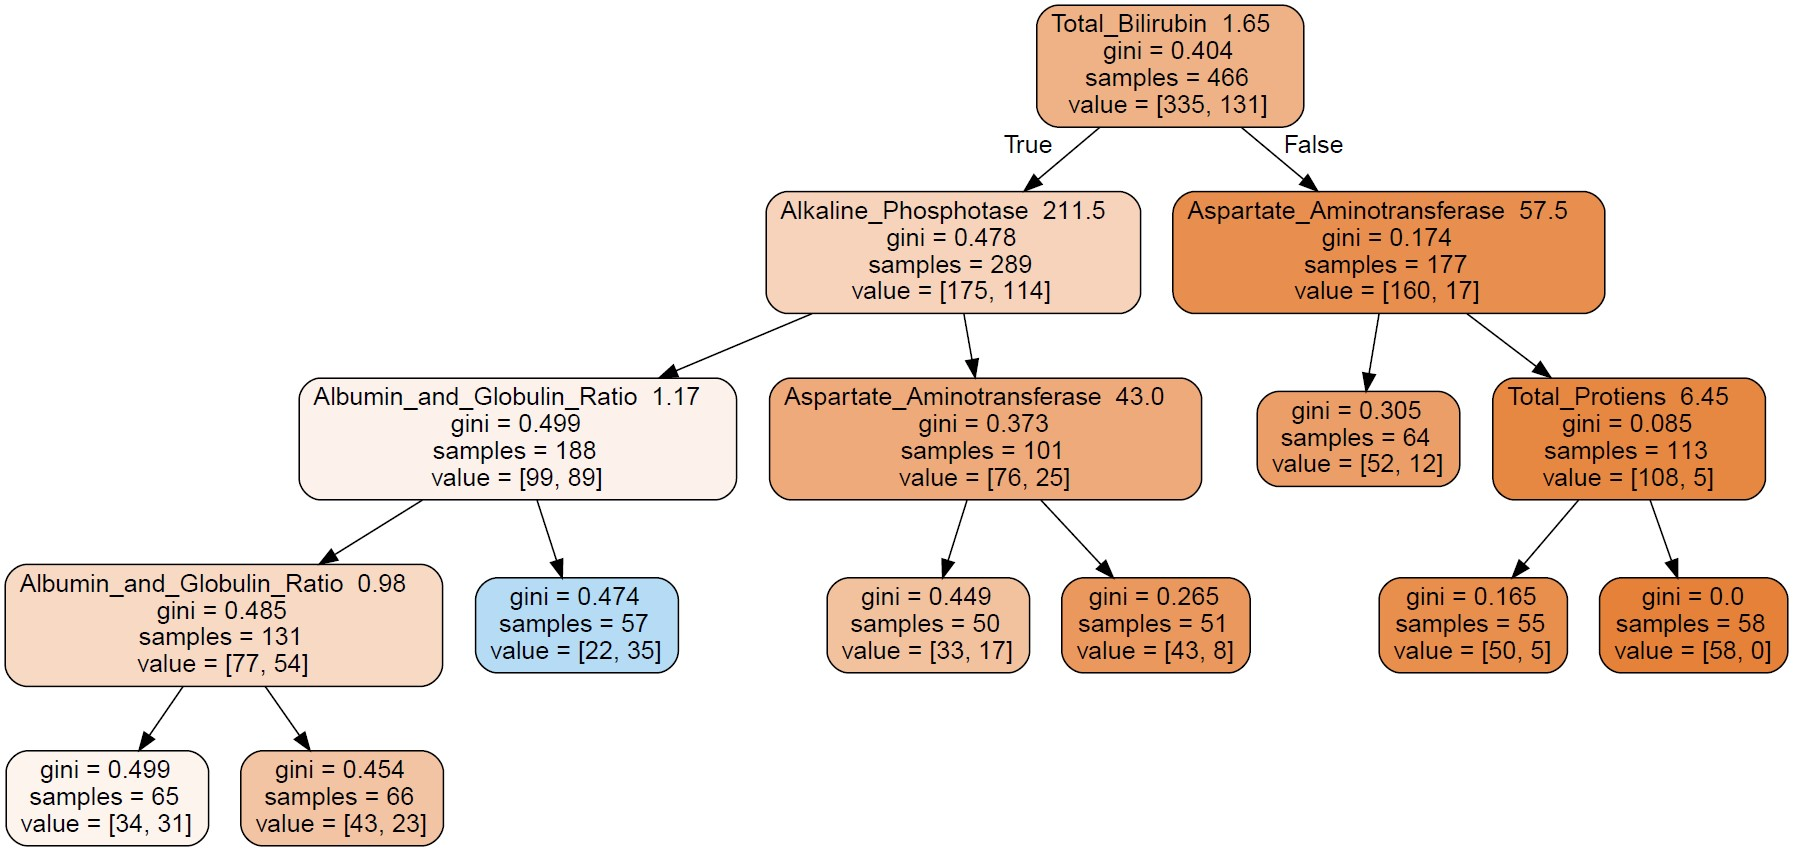
\includegraphics[width=6.45833in,height=5.72917in]{output_660_0.jpg}
\caption{Arbol sklearn (criterion=`gini', splitter=`best',
min\_samples\_split=40, min\_samples\_leaf=50, max\_depth=None,
ccp\_alpha=0)}
\end{figure}

\newpage

Para demostrar que entendemos los parametros que vienen en cada nodo (en
cada recuadro) los vamos a calcular ``manualmente'' para el nodo que se
deriva de True en el nodo raiz, el que tiene como parametros: gini =
0.478 , samples = 289 , value = {[}175, 114{]}

\vspace{0.2cm}

\emph{samples = 289}

\begin{Shaded}
\begin{Highlighting}[]
\NormalTok{df }\OperatorTok{=}\NormalTok{ Data\_Train.loc[Data\_Python[}\StringTok{\textquotesingle{}Total\_Bilirubin\textquotesingle{}}\NormalTok{]}\OperatorTok{\textless{}=}\FloatTok{1.65}\NormalTok{ , :]}
\end{Highlighting}
\end{Shaded}

\begin{Shaded}
\begin{Highlighting}[]
\BuiltInTok{len}\NormalTok{(df)}
\end{Highlighting}
\end{Shaded}

\begin{verbatim}
289
\end{verbatim}

Por tanto, dado un nodo, su parametro \emph{samples} indica el numero de
observaciones de entrenamiento que caerian en la rama que contiene a ese
nodo, si este nodo fuera el nodo terminal de la rama. En el caso
escogido seria la rama definida por Total\_Bilirubin \textless= 1.65.

\vspace{0.2cm}

\emph{value = {[}175, 114{]}}

\begin{Shaded}
\begin{Highlighting}[]
\BuiltInTok{len}\NormalTok{(df.loc[df[}\StringTok{\textquotesingle{}Y\textquotesingle{}}\NormalTok{] }\OperatorTok{==} \DecValTok{0}\NormalTok{ , ])}
\end{Highlighting}
\end{Shaded}

\begin{verbatim}
175
\end{verbatim}

\begin{Shaded}
\begin{Highlighting}[]
\BuiltInTok{len}\NormalTok{(df.loc[df[}\StringTok{\textquotesingle{}Y\textquotesingle{}}\NormalTok{] }\OperatorTok{==} \DecValTok{1}\NormalTok{ , ])}
\end{Highlighting}
\end{Shaded}

\begin{verbatim}
114
\end{verbatim}

Por tanto, dado un nodo, su parametro \emph{value} es un vector con las
frecuencias de las categorias de la variable respuesta (Y) para las
observaciones de train que caerian en la rama que contiene a ese nodo,
si este nodo fuera el nodo terminal de la rama.

\vspace{0.2cm}

\emph{gini = 0.478}

\begin{Shaded}
\begin{Highlighting}[]
\NormalTok{p0 }\OperatorTok{=} \BuiltInTok{len}\NormalTok{(df.loc[df[}\StringTok{\textquotesingle{}Y\textquotesingle{}}\NormalTok{] }\OperatorTok{==} \DecValTok{0}\NormalTok{ , ])}\OperatorTok{/}\BuiltInTok{len}\NormalTok{(df)}
\NormalTok{p1 }\OperatorTok{=} \BuiltInTok{len}\NormalTok{(df.loc[df[}\StringTok{\textquotesingle{}Y\textquotesingle{}}\NormalTok{] }\OperatorTok{==} \DecValTok{1}\NormalTok{ , ])}\OperatorTok{/}\BuiltInTok{len}\NormalTok{(df)}
\end{Highlighting}
\end{Shaded}

\begin{Shaded}
\begin{Highlighting}[]
\NormalTok{p0}\OperatorTok{*}\NormalTok{(}\DecValTok{1}\OperatorTok{{-}}\NormalTok{p0) }\OperatorTok{+}\NormalTok{ p1}\OperatorTok{*}\NormalTok{(}\DecValTok{1}\OperatorTok{{-}}\NormalTok{p1)}
\end{Highlighting}
\end{Shaded}

\begin{verbatim}
0.4777241651800146
\end{verbatim}

Por tanto, dado un nodo del arbol, el parametro \emph{gini} indica el
indice de gini para las observaciones de train que caerian en rama que
contiene a dicho nodo, si este nodo fuera el nodo terminal de dicha
rama.

\newpage

\hypertarget{validaciuxf3n-simple-con-funciuxf3n-de-validacion-propia-y-funcion-classification-tree-de-sklearn}{%
\subsubsection{\texorpdfstring{Validación simple con función de
validacion propia y funcion Classification Tree de
\texttt{sklearn}}{Validación simple con función de validacion propia y funcion Classification Tree de sklearn}}\label{validaciuxf3n-simple-con-funciuxf3n-de-validacion-propia-y-funcion-classification-tree-de-sklearn}}

\begin{Shaded}
\begin{Highlighting}[]
\KeywordTok{def}\NormalTok{ Simple\_Validation\_Classification(Data\_Test, X\_train, Y\_train, Y\_test) :}

    \CommentTok{\#\#\#\#\#\#\#\#\#\#\#\#\#\#\#\#\#\#\#\#\#\#\#\#\#\#}

    \ImportTok{from}\NormalTok{ joblib }\ImportTok{import}\NormalTok{ Parallel, delayed}
    \ImportTok{import}\NormalTok{ multiprocessing}

\NormalTok{    n\_jobs  }\OperatorTok{=}\NormalTok{ multiprocessing.cpu\_count()}

    \CommentTok{\#\#\#\#\#\#\#\#\#\#\#\#\#\#\#\#\#\#\#\#\#\#\#\#\#\#}

\NormalTok{    Classification\_Tree\_sklearn }\OperatorTok{=}\NormalTok{  sklearn.tree.DecisionTreeClassifier(criterion}\OperatorTok{=}\StringTok{\textquotesingle{}gini\textquotesingle{}}\NormalTok{, splitter}\OperatorTok{=}\StringTok{\textquotesingle{}best\textquotesingle{}}\NormalTok{, min\_samples\_split}\OperatorTok{=}\DecValTok{40}\NormalTok{, min\_samples\_leaf}\OperatorTok{=}\DecValTok{50}\NormalTok{,  max\_depth}\OperatorTok{=}\VariableTok{None}\NormalTok{,  ccp\_alpha}\OperatorTok{=}\DecValTok{0}\NormalTok{, random\_state}\OperatorTok{=}\DecValTok{666}\NormalTok{)}
    \CommentTok{\#\#\#\#\#\#\#\#\#\#\#\#\#\#\#\#\#\#\#\#\#\#\#\#\#\#}

    \KeywordTok{def}\NormalTok{ prediction(i, Data\_Test, X\_train, Y\_train ):}

\NormalTok{     x\_new }\OperatorTok{=}\NormalTok{ Data\_Test.iloc[ i , }\BuiltInTok{range}\NormalTok{(}\DecValTok{1}\NormalTok{, Data\_Test.shape[}\DecValTok{1}\NormalTok{])]}

\NormalTok{     Classification\_Tree\_sklearn.fit(X\_train, Y\_train)}

\NormalTok{     y\_new\_predict }\OperatorTok{=}\NormalTok{ Classification\_Tree\_sklearn.predict( [x\_new] ) }
  
     \ControlFlowTok{return}\NormalTok{(y\_new\_predict)}

    \CommentTok{\#\#\#\#\#\#\#\#\#\#\#\#\#\#\#\#\#\#\#\#\#\#\#\#\#\#}

\NormalTok{    y\_predictions\_vector }\OperatorTok{=}\NormalTok{ []}

    \CommentTok{\# Paralelizamos el siguiente bucle for :}

    \CommentTok{\# for i in  range(0, len(Data\_Test)):}

        \CommentTok{\# y\_new\_predict = prediction(i, Data\_Test, X\_train, Y\_train )}

        \CommentTok{\# y\_predictions\_vector.append( y\_new\_predict )}

    
\NormalTok{    y\_predictions\_vector }\OperatorTok{=}\NormalTok{ Parallel(n\_jobs}\OperatorTok{=}\NormalTok{n\_jobs)( delayed(prediction)( i, Data\_Test, X\_train, Y\_train) }\ControlFlowTok{for}\NormalTok{ i }\KeywordTok{in} \BuiltInTok{range}\NormalTok{(}\DecValTok{0}\NormalTok{, }\BuiltInTok{len}\NormalTok{(Data\_Test)) )}

    \CommentTok{\#\#\#\#\#\#\#\#\#\#\#\#\#\#\#\#\#\#\#\#\#\#\#\#\#}

    \ImportTok{from}\NormalTok{ itertools }\ImportTok{import}\NormalTok{ chain}

\NormalTok{    y\_predictions\_vector }\OperatorTok{=} \BuiltInTok{list}\NormalTok{(chain(}\OperatorTok{*}\NormalTok{y\_predictions\_vector))}

 
\NormalTok{    TEC }\OperatorTok{=} \BuiltInTok{sum}\NormalTok{(y\_predictions\_vector }\OperatorTok{!=}\NormalTok{ Y\_test)}\OperatorTok{/}\BuiltInTok{len}\NormalTok{(Y\_test)     }

 
    \ControlFlowTok{return}\NormalTok{(y\_predictions\_vector , TEC)}
\end{Highlighting}
\end{Shaded}

\begin{Shaded}
\begin{Highlighting}[]
\NormalTok{y\_predictions\_vector , TEC\_classification\_tree\_sklearn }\OperatorTok{=}\NormalTok{ Simple\_Validation\_Classification(Data\_Test, X\_train, Y\_train, Y\_test)}
\end{Highlighting}
\end{Shaded}

\begin{Shaded}
\begin{Highlighting}[]
\NormalTok{TEC\_classification\_tree\_sklearn}
\end{Highlighting}
\end{Shaded}

\begin{verbatim}
0.3418803418803419
\end{verbatim}

\newpage

\hypertarget{arboles-de-clasificaciuxf3n-penalizados-en-sklearn-alpha-uxf3ptimo}{%
\subsubsection{\texorpdfstring{4.5.4. Arboles de clasificación
penalizados en \texttt{sklearn} : \(\alpha\) óptimo
}{4.5.4. Arboles de clasificación penalizados en sklearn : \textbackslash alpha óptimo }}\label{arboles-de-clasificaciuxf3n-penalizados-en-sklearn-alpha-uxf3ptimo}}

Vamos a obtener para los datos dados el \(\alpha\) optimo para un arbol
de clasificacion del tipo tipo
sklearn.tree.DecisionTreeClassifier(criterion=`gini', splitter=`best',
random\_state=222)

Es decir para un arbol de clasificacion en el que por defecto
ccp\_alpha=0, min\_samples\_split=2, min\_samples\_leaf=2

\begin{Shaded}
\begin{Highlighting}[]
\NormalTok{Classification\_Tree\_sklearn }\OperatorTok{=}\NormalTok{  sklearn.tree.DecisionTreeClassifier(criterion}\OperatorTok{=}\StringTok{\textquotesingle{}gini\textquotesingle{}}\NormalTok{, splitter}\OperatorTok{=}\StringTok{\textquotesingle{}best\textquotesingle{}}\NormalTok{, ccp\_alpha}\OperatorTok{=}\DecValTok{0}\NormalTok{, random\_state}\OperatorTok{=}\DecValTok{222}\NormalTok{)}

\NormalTok{path }\OperatorTok{=}\NormalTok{ Classification\_Tree\_sklearn.cost\_complexity\_pruning\_path(X\_train, Y\_train)}
\NormalTok{path}
\end{Highlighting}
\end{Shaded}

\begin{verbatim}
{'ccp_alphas': array([0.        , 0.00190749, 0.00190749, 0.00198085, 0.00199264,
        0.00204838, 0.00204838, 0.00208281, 0.00208792, 0.00214592,
        0.00256706, 0.00286123, 0.00286123, 0.00286123, 0.00286123,
        0.00321888, 0.00321888, 0.00321888, 0.00330839, 0.0033381 ,
        0.0033632 , 0.00339575, 0.00343348, 0.00357654, 0.00367872,
        0.00367872, 0.00375536, 0.00375687, 0.00381497, 0.00390878,
        0.00393419, 0.00394962, 0.00398529, 0.00422372, 0.00429185,
        0.0046785 , 0.00525751, 0.00530546, 0.00554939, 0.00566861,
        0.00578789, 0.00579405, 0.00633117, 0.00718679, 0.00983335,
        0.01012134, 0.01438729, 0.0419547 ]),
 'impurities': array([0.        , 0.00381497, 0.00762995, 0.01159165, 0.01557694,
        0.0196737 , 0.02786722, 0.03203284, 0.03620869, 0.03835461,
        0.04862283, 0.05148406, 0.05720652, 0.06006775, 0.06292898,
        0.06614787, 0.06936675, 0.07258564, 0.0891276 , 0.09580381,
        0.10589341, 0.10928915, 0.11272263, 0.11629917, 0.11997789,
        0.12365662, 0.12741198, 0.13116885, 0.1387988 , 0.14661635,
        0.15055054, 0.15844978, 0.16243507, 0.17088251, 0.1794662 ,
        0.19818019, 0.2034377 , 0.21404863, 0.21959801, 0.2762841 ,
        0.28207199, 0.29366009, 0.30632242, 0.3278828 , 0.33771614,
        0.34783749, 0.36222478, 0.40417948])}
\end{verbatim}

\begin{Shaded}
\begin{Highlighting}[]
\NormalTok{ccp\_alphas, impurities }\OperatorTok{=}\NormalTok{ path.ccp\_alphas, path.impurities}
\end{Highlighting}
\end{Shaded}

\begin{Shaded}
\begin{Highlighting}[]
\NormalTok{Classification\_Tree\_sklearn\_vector }\OperatorTok{=}\NormalTok{ []}

\ControlFlowTok{for}\NormalTok{ ccp\_alpha }\KeywordTok{in}\NormalTok{ ccp\_alphas:}
    
\NormalTok{    Classification\_Tree\_sklearn }\OperatorTok{=}\NormalTok{ DecisionTreeClassifier(ccp\_alpha}\OperatorTok{=}\NormalTok{ccp\_alpha, criterion}\OperatorTok{=}\StringTok{\textquotesingle{}gini\textquotesingle{}}\NormalTok{, splitter}\OperatorTok{=}\StringTok{\textquotesingle{}best\textquotesingle{}}\NormalTok{, random\_state}\OperatorTok{=}\DecValTok{222}\NormalTok{)}
    
\NormalTok{    Classification\_Tree\_sklearn.fit(X\_train, Y\_train)}

\NormalTok{    Classification\_Tree\_sklearn\_vector.append(Classification\_Tree\_sklearn)}
\end{Highlighting}
\end{Shaded}

\begin{Shaded}
\begin{Highlighting}[]
\ImportTok{from}\NormalTok{ sklearn.metrics }\ImportTok{import}\NormalTok{ accuracy\_score}
\end{Highlighting}
\end{Shaded}

\begin{Shaded}
\begin{Highlighting}[]
\NormalTok{acc\_scores }\OperatorTok{=}\NormalTok{ [accuracy\_score(Y\_test, Classification\_Tree\_sklearn.predict(X\_test)) }\ControlFlowTok{for}\NormalTok{ Classification\_Tree\_sklearn }\KeywordTok{in}\NormalTok{ Classification\_Tree\_sklearn\_vector]}

\NormalTok{ramas }\OperatorTok{=}\NormalTok{ [Classification\_Tree\_sklearn.get\_n\_leaves() }\ControlFlowTok{for}\NormalTok{ Classification\_Tree\_sklearn }\KeywordTok{in}\NormalTok{ Classification\_Tree\_sklearn\_vector]}
\end{Highlighting}
\end{Shaded}

\begin{Shaded}
\begin{Highlighting}[]
\ImportTok{import}\NormalTok{ matplotlib.pyplot }\ImportTok{as}\NormalTok{ plt}

\NormalTok{plt.figure(figsize}\OperatorTok{=}\NormalTok{(}\DecValTok{9}\NormalTok{,  }\DecValTok{9}\NormalTok{))}
\NormalTok{plt.grid()}
\NormalTok{plt.plot(ccp\_alphas[:}\OperatorTok{{-}}\DecValTok{1}\NormalTok{], acc\_scores[:}\OperatorTok{{-}}\DecValTok{1}\NormalTok{], color}\OperatorTok{=}\StringTok{\textquotesingle{}red\textquotesingle{}}\NormalTok{)}
\NormalTok{plt.xlabel(}\StringTok{"alpha"}\NormalTok{)}
\NormalTok{plt.ylabel(}\StringTok{"score (TAC = 1 {-} TEC)"}\NormalTok{)}
\end{Highlighting}
\end{Shaded}

\begin{figure}
\centering
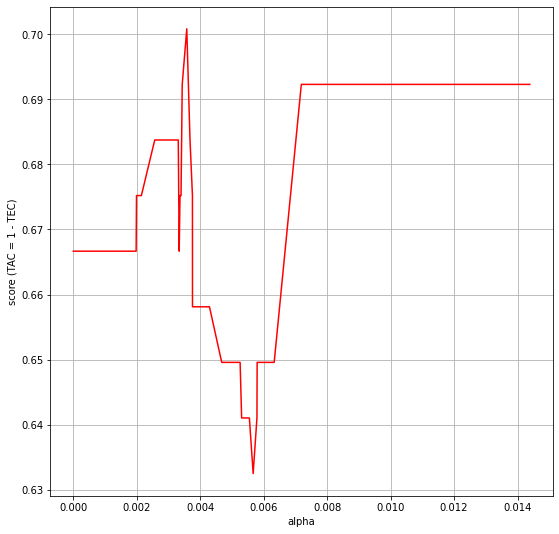
\includegraphics[width=6.25in,height=5.20833in]{output_695_1.png}
\caption{TAC vs \(\alpha\)}
\end{figure}

\newpage

\begin{Shaded}
\begin{Highlighting}[]
\NormalTok{alpha\_score\_df }\OperatorTok{=}\NormalTok{ pd.DataFrame(\{}\StringTok{\textquotesingle{}alpha\textquotesingle{}}\NormalTok{:ccp\_alphas, }\StringTok{\textquotesingle{}score (TAC = 1{-}TEC)\textquotesingle{}}\NormalTok{: acc\_scores , }\StringTok{\textquotesingle{}ramas\textquotesingle{}}\NormalTok{: ramas\})}
\end{Highlighting}
\end{Shaded}

\begin{Shaded}
\begin{Highlighting}[]
\NormalTok{alpha\_score\_df\_sorted }\OperatorTok{=}\NormalTok{ alpha\_score\_df.sort\_values(by}\OperatorTok{=}\NormalTok{[}\StringTok{"score (TAC = 1{-}TEC)"}\NormalTok{], ascending}\OperatorTok{=}\VariableTok{False}\NormalTok{).reset\_index(drop}\OperatorTok{=}\VariableTok{False}\NormalTok{)}
\NormalTok{alpha\_score\_df\_sorted[}\StringTok{\textquotesingle{}TEC\textquotesingle{}}\NormalTok{]}\OperatorTok{=} \DecValTok{1} \OperatorTok{{-}}\NormalTok{ alpha\_score\_df\_sorted[}\StringTok{\textquotesingle{}score (TAC = 1{-}TEC)\textquotesingle{}}\NormalTok{]}
\end{Highlighting}
\end{Shaded}

\begin{Shaded}
\begin{Highlighting}[]
\NormalTok{alpha\_score\_df\_sorted.head(}\DecValTok{7}\NormalTok{)}
\end{Highlighting}
\end{Shaded}

\begin{verbatim}
       index       alpha      score (TAC = 1-TEC)     ramas       TEC
0        23      0.003577             0.700855         47       0.299145
1        47      0.041955             0.692308         1        0.307692
2        46      0.014387             0.692308         2        0.307692
3        45      0.010121             0.692308         3        0.307692
4        44      0.009833             0.692308         4        0.307692
5        43      0.007187             0.692308         5        0.307692
6        22      0.003433             0.692308         48       0.307692
\end{verbatim}

\vspace{0.5cm}

\textbf{Validacion simple con \(\alpha\) óptimo:}

\begin{Shaded}
\begin{Highlighting}[]
\KeywordTok{def}\NormalTok{ Simple\_Validation\_Classification(Data\_Test, X\_train, Y\_train, Y\_test) :}

    \CommentTok{\#\#\#\#\#\#\#\#\#\#\#\#\#\#\#\#\#\#\#\#\#\#\#\#\#\#}

    \ImportTok{from}\NormalTok{ joblib }\ImportTok{import}\NormalTok{ Parallel, delayed}
    \ImportTok{import}\NormalTok{ multiprocessing}

\NormalTok{    n\_jobs  }\OperatorTok{=}\NormalTok{ multiprocessing.cpu\_count()}

    \CommentTok{\#\#\#\#\#\#\#\#\#\#\#\#\#\#\#\#\#\#\#\#\#\#\#\#\#\#}

\NormalTok{    Classification\_Tree\_penalized\_star }\OperatorTok{=}\NormalTok{ sklearn.tree.DecisionTreeClassifier(ccp\_alpha}\OperatorTok{=}\NormalTok{alpha\_score\_df\_sorted[}\StringTok{\textquotesingle{}alpha\textquotesingle{}}\NormalTok{][}\DecValTok{0}\NormalTok{], criterion}\OperatorTok{=}\StringTok{\textquotesingle{}gini\textquotesingle{}}\NormalTok{, splitter}\OperatorTok{=}\StringTok{\textquotesingle{}best\textquotesingle{}}\NormalTok{, random\_state}\OperatorTok{=}\DecValTok{222}\NormalTok{)}
    \CommentTok{\#\#\#\#\#\#\#\#\#\#\#\#\#\#\#\#\#\#\#\#\#\#\#\#\#\#}

    \KeywordTok{def}\NormalTok{ prediction(i, Data\_Test, X\_train, Y\_train ):}

\NormalTok{     x\_new }\OperatorTok{=}\NormalTok{ Data\_Test.iloc[ i , }\BuiltInTok{range}\NormalTok{(}\DecValTok{1}\NormalTok{, Data\_Test.shape[}\DecValTok{1}\NormalTok{])]}

\NormalTok{     Classification\_Tree\_penalized\_star.fit(X\_train, Y\_train)}

\NormalTok{     y\_new\_predict }\OperatorTok{=}\NormalTok{ Classification\_Tree\_penalized\_star.predict( [x\_new] ) }
  
     \ControlFlowTok{return}\NormalTok{(y\_new\_predict)}

    \CommentTok{\#\#\#\#\#\#\#\#\#\#\#\#\#\#\#\#\#\#\#\#\#\#\#\#\#\#}

\NormalTok{    y\_predictions\_vector }\OperatorTok{=}\NormalTok{ []}

    \CommentTok{\# Paralelizamos el siguiente bucle for :}

    \CommentTok{\# for i in  range(0, len(Data\_Test)):}

        \CommentTok{\# y\_new\_predict = prediction(i, Data\_Test, X\_train, Y\_train )}

        \CommentTok{\# y\_predictions\_vector.append( y\_new\_predict )}

    
\NormalTok{    y\_predictions\_vector }\OperatorTok{=}\NormalTok{ Parallel(n\_jobs}\OperatorTok{=}\NormalTok{n\_jobs)( delayed(prediction)( i, Data\_Test, X\_train, Y\_train) }\ControlFlowTok{for}\NormalTok{ i }\KeywordTok{in} \BuiltInTok{range}\NormalTok{(}\DecValTok{0}\NormalTok{, }\BuiltInTok{len}\NormalTok{(Data\_Test)) )}

    \CommentTok{\#\#\#\#\#\#\#\#\#\#\#\#\#\#\#\#\#\#\#\#\#\#\#\#\#}

    \ImportTok{from}\NormalTok{ itertools }\ImportTok{import}\NormalTok{ chain}

\NormalTok{    y\_predictions\_vector }\OperatorTok{=} \BuiltInTok{list}\NormalTok{(chain(}\OperatorTok{*}\NormalTok{y\_predictions\_vector))}

 
\NormalTok{    TEC }\OperatorTok{=} \BuiltInTok{sum}\NormalTok{(y\_predictions\_vector }\OperatorTok{!=}\NormalTok{ Y\_test)}\OperatorTok{/}\BuiltInTok{len}\NormalTok{(Y\_test)    }

 
    \ControlFlowTok{return}\NormalTok{(y\_predictions\_vector , TEC)}
\end{Highlighting}
\end{Shaded}

\vspace{0.25cm}

\begin{Shaded}
\begin{Highlighting}[]
\NormalTok{y\_predictions\_vector , TEC\_classification\_tree\_penalized\_star }\OperatorTok{=}\NormalTok{ Simple\_Validation\_Classification(Data\_Test, X\_train, Y\_train, Y\_test)}
\end{Highlighting}
\end{Shaded}

\begin{Shaded}
\begin{Highlighting}[]
\NormalTok{TEC\_classification\_tree\_penalized\_star}
\end{Highlighting}
\end{Shaded}

\begin{verbatim}
0.29914529914529914
\end{verbatim}

\newpage

\hypertarget{comparaciuxf3n-final-entre-uxe1rboles-de-clasificaciuxf3n-por-validaciuxf3n-simple}{%
\subsubsection{\texorpdfstring{4.5.5. Comparación final entre árboles de
clasificación por validación simple
}{4.5.5. Comparación final entre árboles de clasificación por validación simple }}\label{comparaciuxf3n-final-entre-uxe1rboles-de-clasificaciuxf3n-por-validaciuxf3n-simple}}

\begin{Shaded}
\begin{Highlighting}[]
\NormalTok{[TEC\_classification\_tree\_penalized\_star , TEC\_classification\_tree\_sklearn, TEC\_classification\_tree\_own\_function, TEC\_classification\_tree\_Gini\_own\_function,]}
\end{Highlighting}
\end{Shaded}

\begin{verbatim}
[0.29914529914529914,
 0.3418803418803419,
 0.3076923076923077,
 0.28205128205128205]
\end{verbatim}

El ranking de modelos segun validacion simple sería :

\begin{enumerate}
\def\labelenumi{\arabic{enumi}.}
\item
  TEC\_classification\_tree\_Gini\_own\_function
\item
  TEC\_classification\_tree\_penalized\_star(ccp\_alpha=alpha\_score\_df\_sorted{[}`alpha'{]}{[}0{]}
  , criterion=`gini', splitter=`best', random\_state=222))
\item
  TEC\_classification\_tree\_own\_function
\item
  TEC\_classification\_tree\_sklearn
  (DecisionTreeRegressor(criterion=`gini', splitter=`best',
  min\_samples\_split=40, min\_samples\_leaf=50, max\_depth=None,
  ccp\_alpha=0, random\_state=222) )
\end{enumerate}

\newpage

\#\#. KNN para clasificación en \texttt{Python}

\hypertarget{knn-para-clasificaciuxf3n-teoruxeda}{%
\subsubsection{KNN para clasificación:
teoría}\label{knn-para-clasificaciuxf3n-teoruxeda}}

\begin{itemize}
\item
  Tenemos \(\hspace{0.1cm} p \hspace{0.1cm}\) variables
  \(\hspace{0.1cm} X=(X_1,...,X_p) \hspace{0.1cm}\) medidas en un \(n\)
  muestra de tamaño.
\item
  También tenemos una variable de respuesta \textbf{categórica}
  \(\hspace{0.1cm} Y \hspace{0.1cm}\) con
  \(\hspace{0.1cm} g \hspace{0.1cm}\) categorías que indica el grupo al
  que cada elemento de la muestra pertenece
  \(( \hspace{0.05cm} Range(Y)=\lbrace c_1 ,..., c_g \rbrace \hspace{0.05cm})\)
\item
  Los grupos generados por \(\hspace{0.1cm} Y \hspace{0.1cm}\) se
  denotan como
  \(\hspace{0.1cm} \Omega_1 ,..., \Omega_g \hspace{0.15cm}\)
  \(\hspace{ 0.15cm}( \hspace{0.1cm} y_i = c_r \hspace{0.15cm} \Leftrightarrow \hspace{0.15cm}\)
  \(i \in \Omega_r \hspace{0.1cm})\)
\end{itemize}

\vspace{0.3cm}

El problema de clasificación supervisada consiste en, para una nueva
observación de las variables \(X_1,...,X_p \hspace{0.1cm}\),
\(\hspace{0.1cm} x_{nueva} = (x_{nueva,1}\ hspace{0.1cm},\hspace{0.1cm}x_{nuevo,2}\hspace{0.1cm},\dots,\hspace{0.1cm}x_{nuevo,p}) \hspace{0.1cm}\),
predecir es \(\hspace{0.1cm} Y \hspace{0.1cm}\) valor
\(\hspace{0.1cm} (y_{nuevo})\hspace{0.1cm}\) usando la información
disponible de \(\hspace{0.1cm} X_1 ,...,X_p \hspace{0.1cm}\) y \$
\hspace{0.1cm} Y\$

Entonces, el problema es clasificar un nuevo elemento/individuo en uno
de los \(\hspace{0.1cm} g \hspace{0.1cm}\) grupos generados por
\(\hspace{0.1cm} Y \hspace{0.1cm}\) usando la información disponible de
\(\hspace{0.1cm} X_1,...,X_p \hspace{0.1cm}\) y \(Y\), y también
\(\hspace{0.1cm} x_{nuevo} = (x_{nuevo,1 }\hspace{0.1cm},\hspace{0.1cm}x_{nuevo,2}\hspace{0.1cm},\dots,\hspace{0.1cm}x_{nuevo,p}) \hspace{0.1cm}\)

Tengase en cuenta que si no tenemos información sobre
\(\hspace{0.1cm} Y \hspace{0.1cm}\), esto sería un problema de
clasificación no supervisado.

\vspace{0.3cm}

El algoritmo KNN (K-vecinos más cercanos) para la clasificación
supervisada tiene los siguientes pasos:

\vspace{0.2cm}

\(1. \hspace{0.15cm}\) Define una medida de \textbf{distancia} entre las
observaciones de la muestra original respecto a las variables
\(X_1,...,X_p\) \(\hspace{0.15cm} \Rightarrow \hspace{0.15cm}\)
\(\delta\)

\vspace{0.2cm}

\(2. \hspace{0.15cm}\) Calcula las distancias entre
\(\hspace{0.1 cm}x_{new}\hspace{0.1 cm}\) y las observaciones iniciales
\(\hspace{0.1cm} \lbrace x_1,...,x_n \rbrace\)
\(\hspace{0.15cm} \Rightarrow \hspace{0.15cm}\)
\(\lbrace \hspace{0.1 cm} \delta(x_{nuevo}\hspace{0.03 cm},\hspace{0.03 cm} x_i) \hspace{0.1 cm} / \hspace{0.1 cm} i=1,...,n \hspace{0.1 cm} \rbrace\)

\vspace{0.2cm}

\(3. \hspace{0.15cm}\) Seleccione la
\(\hspace{0.03 cm} k \hspace{0.03 cm}\) observación más cercana a
\(\hspace{0.06 cm} x_{nuevo}\hspace{0.06 cm}\) basado en
\(\hspace {0.05cm} \delta \hspace{0.12cm}\) \((k\) vecinos más cercanos
de \(x_{nuevo})\) \(\hspace{0.15cm} \Rightarrow \hspace{0.15cm}\) El
conjunto de estas observaciones será denotar por \(KNN(x_{nuevo})\)

\vspace{0.2cm}

\(4. \hspace{0.15cm}\) Calcular la proporción de estas observaciones
(vecinos) que pertenecen a cada grupo :

La proporción de \(KNN\) que pertenece al grupo
\(\hspace{0.15cm} \Omega_r\) \(\hspace{0.1cm}(Y=c_r) \hspace{0.1cm}\)
será denotado por \(\hspace{0.1 cm} f^{knn}_{r}\)

\[\hspace{0.1 cm} f^{KNN(x_{new})}_{r} \hspace{0.15cm}=\hspace{0.15cm} \dfrac{ \# \hspace{0.1cm}\lbrace\hspace{0.1cm} i \in KNN(x_{new}) \hspace{0.1cm}/\hspace{0.1cm} i \in \Omega_r \hspace{0.1cm}\rbrace  }{\# \hspace{0.1cm} KNN(x_{new}) = k} \hspace{0.15cm}=\hspace{0.15cm}  \dfrac{ \# \hspace{0.1cm}\lbrace\hspace{0.1cm} i \in KNN \hspace{0.1cm}/\hspace{0.1cm} y_i = r \hspace{0.1cm}\rbrace  }{ k}\]

\vspace{0.2cm}

\(5. \hspace{0.15cm}\) Clasifica
\(\hspace{0.1cm} x_{new} \hspace{0.1cm}\) en ese grupo/clase \((\)
definido por \(Y)\) más frecuente en KNN:

\(\hspace{0.25cm} \hspace{0.2cm}\)
\(\text{If} \hspace{0.15cm} \underbrace{ f^{knn}_{s} \geqslant f^{knn}_{r} \hspace{0.15cm},\hspace{0.15cm} \forall r = 1,...,g }_{s \hspace{0.1cm}\text{es la clase más frecuente en}\hspace{0.1cm} KNN }\)
\(\hspace{0.1cm} \hspace{0.15cm} \Rightarrow \hspace{0.15cm} x_{new} \hspace{0.1cm}\)
se clasifica en \(\hspace{0.1cm} \Omega_s\)
\(\hspace{0.15cm} \Rightarrow \hspace{0.15cm} \widehat{y}_{new} = s\)

\vspace{0.2cm}

\(\hspace{0.2 cm}\) En otras palabras:

\(\hspace{0.6 cm} \text{If} \hspace{0.4 cm} s^* \hspace{0.05 cm}= \hspace{0.05 cm} \underset{\hspace{0.7 cm} s}{arg \hspace{ 0.1 cm} Máx.} \hspace{0.05 cm} \left(\hspace{0.1 cm} f^{KNN(x_{new})}_{s} \hspace{0.1 cm}\right) \hspace{0.2 cm} \hspace{0.15cm} \Rightarrow \hspace{0.25cm} \widehat{y}_{new} = s^* \hspace{0.1cm}\)

\newpage

\hypertarget{algoritmo-de-creaciuxf3n-proia-en-python}{%
\subsubsection{\texorpdfstring{4.6.2. Algoritmo de creación proia en
\texttt{Python}
}{4.6.2. Algoritmo de creación proia en Python }}\label{algoritmo-de-creaciuxf3n-proia-en-python}}

Vamos a desarrollar nuestro propio algoritmo para no depender de sklearn

\begin{Shaded}
\begin{Highlighting}[]
\KeywordTok{def}\NormalTok{ KNN\_classification( X , Y , x\_new, k, distance }\OperatorTok{=} \StringTok{"Minkowski"}\NormalTok{ , q }\OperatorTok{=} \DecValTok{0}\NormalTok{, p1}\OperatorTok{=}\DecValTok{0}\NormalTok{, p2}\OperatorTok{=}\DecValTok{0}\NormalTok{, p3}\OperatorTok{=}\DecValTok{0}\NormalTok{ ):}

    
\CommentTok{\#\# Para paralelizar el algoritmo }

    \ImportTok{from}\NormalTok{ joblib }\ImportTok{import}\NormalTok{ Parallel, delayed}
    \ImportTok{import}\NormalTok{ multiprocessing}

\NormalTok{    n\_jobs  }\OperatorTok{=}\NormalTok{ multiprocessing.cpu\_count()}

\CommentTok{\#\#\#\#\#\#\#\#\#\#\#\#\#\#\#\#\#\#\#\#\#\#\#\#\#\#\#\#\#\#\#\#\#\#\#\#\#\#\#\#\#\#\#\#\#\#\#\#\#\#\#\#\#\#\#\#\#\#\#\#\#}

    \CommentTok{\# Y, X y x\_new deben ser objetos Pandas ya que luego seran convertidos a objetos Numpy automaticamente por el algoritmo}
    
    \CommentTok{\# Y tiene que ser un Pandas data frame con la variable respuesta (que en este caso debe ser categorica y con categorias estandar \{0,1,2,...\}) }

    \CommentTok{\# X tiene que ser un Pandas data frame con los predictotres (X1,...,Xp). }

    \CommentTok{\# x\_new tiene que ser un vector con una nueva observacion de los predictores. }


\CommentTok{\#\#\#\#\#\#\#\#\#\#\#\#\#\#\#\#\#\#\#\#\#\#\#\#\#\#\#\#\#\#\#\#\#\#\#\#\#\#\#\#\#\#\#\#\#\#\#\#\#\#\#\#\#\#\#\#\#\#\#\#\#}

\NormalTok{    Y }\OperatorTok{=}\NormalTok{ Y.to\_numpy()}

\NormalTok{    X }\OperatorTok{=}\NormalTok{ X.to\_numpy() }

\NormalTok{    x\_new }\OperatorTok{=}\NormalTok{ x\_new.to\_numpy()}

\NormalTok{    X }\OperatorTok{=}\NormalTok{ np.concatenate((X, [x\_new]), axis}\OperatorTok{=}\DecValTok{0}\NormalTok{)}


\NormalTok{    distances }\OperatorTok{=}\NormalTok{ []}

\NormalTok{    groups\_knn }\OperatorTok{=}\NormalTok{ []}

\CommentTok{\#\#\#\#\#\#\#\#\#\#\#\#\#\#\#\#\#\#\#\#\#\#\#\#\#\#\#\#\#\#\#\#\#\#\#\#\#\#\#\#\#\#\#\#\#\#\#\#\#\#\#\#\#\#\#\#\#\#\#\#\#\#\#}
    
    \KeywordTok{def}\NormalTok{ a(Binary\_Data) :}

\NormalTok{            X }\OperatorTok{=}\NormalTok{ Binary\_Data}

\NormalTok{            a }\OperatorTok{=}\NormalTok{ X }\OperatorTok{@}\NormalTok{ X.T}

            \ControlFlowTok{return}\NormalTok{(a)}

\CommentTok{\#\#\#\#\#\#\#\#\#\#\#\#\#\#\#\#\#\#\#\#\#\#\#\#\#\#\#\#\#\#\#\#\#\#\#\#\#\#\#\#\#\#\#\#\#\#\#\#\#\#\#\#\#\#\#\#\#\#\#\#\#\#\#}

    \KeywordTok{def}\NormalTok{ d(Binary\_Data):}

\NormalTok{            X }\OperatorTok{=}\NormalTok{ Binary\_Data}

\NormalTok{            ones\_matrix }\OperatorTok{=}\NormalTok{ np.ones(( X.shape[}\DecValTok{0}\NormalTok{] , X.shape[}\DecValTok{1}\NormalTok{])) }

\NormalTok{            d }\OperatorTok{=}\NormalTok{ (ones\_matrix }\OperatorTok{{-}}\NormalTok{ X) }\OperatorTok{@}\NormalTok{ (ones\_matrix }\OperatorTok{{-}}\NormalTok{ X).T}

            \ControlFlowTok{return}\NormalTok{(d)}

\CommentTok{\#\#\#\#\#\#\#\#\#\#\#\#\#\#\#\#\#\#\#\#\#\#\#\#\#\#\#\#\#\#\#\#\#\#\#\#\#\#\#\#\#\#\#\#\#\#\#\#\#\#\#\#\#\#\#\#\#\#\#\#\#\#\#}

    \KeywordTok{def}\NormalTok{ alpha\_py(i,j, Multiple\_Categorical\_Data):}

\NormalTok{        X }\OperatorTok{=}\NormalTok{ Multiple\_Categorical\_Data}

\NormalTok{        alpha }\OperatorTok{=}\NormalTok{ np.repeat(}\DecValTok{0}\NormalTok{, X.shape[}\DecValTok{1}\NormalTok{])}

        \ControlFlowTok{for}\NormalTok{ k }\KeywordTok{in} \BuiltInTok{range}\NormalTok{(}\DecValTok{0}\NormalTok{, X.shape[}\DecValTok{1}\NormalTok{]) :}

            \ControlFlowTok{if}\NormalTok{ X[i}\OperatorTok{{-}}\DecValTok{1}\NormalTok{, k] }\OperatorTok{==}\NormalTok{ X[j}\OperatorTok{{-}}\DecValTok{1}\NormalTok{, k] :}

\NormalTok{                alpha[k] }\OperatorTok{=} \DecValTok{1}

            \ControlFlowTok{else}\NormalTok{ :}

\NormalTok{                alpha[k] }\OperatorTok{=} \DecValTok{0}

\NormalTok{        alpha }\OperatorTok{=}\NormalTok{ alpha.}\BuiltInTok{sum}\NormalTok{()}

        \ControlFlowTok{return}\NormalTok{(alpha)}

\CommentTok{\#\#\#\#\#\#\#\#\#\#\#\#\#\#\#\#\#\#\#\#\#\#\#\#\#\#\#\#\#\#\#\#\#\#\#\#\#\#\#\#\#\#\#\#\#\#\#\#\#\#\#\#\#\#\#\#\#\#\#\#\#\#\#    }
    \ControlFlowTok{if}\NormalTok{ distance }\OperatorTok{==} \StringTok{"Euclidean"}\NormalTok{:}

        \KeywordTok{def}\NormalTok{ Dist\_Euclidea\_Python(i, j, Quantitative\_Data\_set): }

\NormalTok{            Dist\_Euclidea }\OperatorTok{=}\NormalTok{ ( ( Quantitative\_Data\_set[i}\OperatorTok{{-}}\DecValTok{1}\NormalTok{, :] }\OperatorTok{{-}}\NormalTok{ Quantitative\_Data\_set[j}\OperatorTok{{-}}\DecValTok{1}\NormalTok{, :] )}\OperatorTok{**}\DecValTok{2}\NormalTok{ ).}\BuiltInTok{sum}\NormalTok{()}

\NormalTok{            Dist\_Euclidea }\OperatorTok{=}\NormalTok{ np.sqrt(Dist\_Euclidea)}

            \ControlFlowTok{return}\NormalTok{ Dist\_Euclidea}

\CommentTok{\#\#\#\#\#\#\#\#\#\#\#\#\#\#\#\#\#\#\#\#\#\#\#\#\#\#\#\#\#\#\#\#\#\#\#\#\#\#\#\#\#\#\#\#\#\#\#\#\#\#\#\#\#\#\#\#\#\#\#\#\#\#\#}
           
        \CommentTok{\#\# PARTE DEL CODIGO A PARALELIZAR}

        \CommentTok{\#for j in range(1, len(X)):}

          \CommentTok{\# distances.append( Dist\_Euclidea\_Python( len(X), i , X ) )}

\NormalTok{        n\_jobs  }\OperatorTok{=}\NormalTok{ multiprocessing.cpu\_count()}

\NormalTok{        distances }\OperatorTok{=}\NormalTok{ Parallel(n\_jobs}\OperatorTok{=}\NormalTok{n\_jobs)( delayed(Dist\_Euclidea\_Python)( }\BuiltInTok{len}\NormalTok{(X), s , X ) }\ControlFlowTok{for}\NormalTok{ s }\KeywordTok{in} \BuiltInTok{range}\NormalTok{(}\DecValTok{1}\NormalTok{, }\BuiltInTok{len}\NormalTok{(X)) )}
           

\CommentTok{\#\#\#\#\#\#\#\#\#\#\#\#\#\#\#\#\#\#\#\#\#\#\#\#\#\#\#\#\#\#\#\#\#\#\#\#\#\#\#\#\#\#\#\#\#\#\#\#\#\#\#\#\#\#\#\#\#\#\#\#\#\#\#}

    \ControlFlowTok{if}\NormalTok{ distance }\OperatorTok{==} \StringTok{"Minkowski"}\NormalTok{:}

        \KeywordTok{def}\NormalTok{ Dist\_Minkowski\_Python(i,j, q , Quantitative\_Data\_set):}

\NormalTok{            Dist\_Minkowski }\OperatorTok{=}\NormalTok{ ( ( ( }\BuiltInTok{abs}\NormalTok{( Quantitative\_Data\_set[i}\OperatorTok{{-}}\DecValTok{1}\NormalTok{, :] }\OperatorTok{{-}}\NormalTok{ Quantitative\_Data\_set[j}\OperatorTok{{-}}\DecValTok{1}\NormalTok{, :] ) )}\OperatorTok{**}\NormalTok{q ).}\BuiltInTok{sum}\NormalTok{() )}\OperatorTok{**}\NormalTok{(}\DecValTok{1}\OperatorTok{/}\NormalTok{q)}

            \ControlFlowTok{return}\NormalTok{ Dist\_Minkowski}

\CommentTok{\#\#\#\#\#\#\#\#\#\#\#\#\#\#\#\#\#\#\#\#\#\#\#\#\#\#\#\#\#\#\#\#\#\#\#\#\#\#\#\#\#\#\#\#\#\#\#\#\#\#\#\#\#\#\#\#\#\#\#\#\#\#\#}

        \CommentTok{\#\# PARTE DEL CODIGO A PARALELIZAR}

        \CommentTok{\# for i in range(1, len(X)):}

          \CommentTok{\#  distances.append( Dist\_Minkowski\_Python( len(X), i , q , X) )}

\NormalTok{        n\_jobs  }\OperatorTok{=}\NormalTok{ multiprocessing.cpu\_count()}

\NormalTok{        distances }\OperatorTok{=}\NormalTok{ Parallel(n\_jobs}\OperatorTok{=}\NormalTok{n\_jobs)( delayed(Dist\_Minkowski\_Python)( }\BuiltInTok{len}\NormalTok{(X), s , q , X) }\ControlFlowTok{for}\NormalTok{ s }\KeywordTok{in} \BuiltInTok{range}\NormalTok{(}\DecValTok{1}\NormalTok{, }\BuiltInTok{len}\NormalTok{(X)) )}

\CommentTok{\#\#\#\#\#\#\#\#\#\#\#\#\#\#\#\#\#\#\#\#\#\#\#\#\#\#\#\#\#\#\#\#\#\#\#\#\#\#\#\#\#\#\#\#\#\#\#\#\#\#\#\#\#\#\#\#\#\#\#\#\#\#\#}

    \ControlFlowTok{if}\NormalTok{ distance }\OperatorTok{==} \StringTok{"Canberra"}\NormalTok{:}

        \KeywordTok{def}\NormalTok{ Dist\_Canberra\_Python(i,j, Quantitative\_Data\_set):}

\NormalTok{            numerator }\OperatorTok{=}  \BuiltInTok{abs}\NormalTok{( Quantitative\_Data\_set[i}\OperatorTok{{-}}\DecValTok{1}\NormalTok{, :] }\OperatorTok{{-}}\NormalTok{ Quantitative\_Data\_set[j}\OperatorTok{{-}}\DecValTok{1}\NormalTok{, :] )  }

\NormalTok{            denominator }\OperatorTok{=}\NormalTok{  ( }\BuiltInTok{abs}\NormalTok{(Quantitative\_Data\_set[i}\OperatorTok{{-}}\DecValTok{1}\NormalTok{, :]) }\OperatorTok{+} \BuiltInTok{abs}\NormalTok{(Quantitative\_Data\_set[j}\OperatorTok{{-}}\DecValTok{1}\NormalTok{, :]) )}
       
\NormalTok{            numerator}\OperatorTok{=}\NormalTok{np.array([numerator], dtype}\OperatorTok{=}\BuiltInTok{float}\NormalTok{)}

\NormalTok{            denominator}\OperatorTok{=}\NormalTok{np.array([denominator], dtype}\OperatorTok{=}\BuiltInTok{float}\NormalTok{)}

\NormalTok{            Dist\_Canberra }\OperatorTok{=}\NormalTok{ ( np.divide( numerator , denominator , out}\OperatorTok{=}\NormalTok{np.zeros\_like(numerator), where}\OperatorTok{=}\NormalTok{denominator}\OperatorTok{!=}\DecValTok{0}\NormalTok{) ).}\BuiltInTok{sum}\NormalTok{()}

            \ControlFlowTok{return}\NormalTok{ Dist\_Canberra}

\CommentTok{\#\#\#\#\#\#\#\#\#\#\#\#\#\#\#\#\#\#\#\#\#\#\#\#\#\#\#\#\#\#\#\#\#\#\#\#\#\#\#\#\#\#\#\#\#\#\#\#\#\#\#\#\#\#\#\#\#\#\#\#\#\#\#}

        \CommentTok{\#\# PARTE DEL CODIGO A PARALELIZAR}

        \CommentTok{\# for i in range(1, len(X)):}

          \CommentTok{\#  distances.append( Dist\_Canberra\_Python( len(X), i , X) )}

\NormalTok{        n\_jobs  }\OperatorTok{=}\NormalTok{ multiprocessing.cpu\_count()}

\NormalTok{        distances }\OperatorTok{=}\NormalTok{ Parallel(n\_jobs}\OperatorTok{=}\NormalTok{n\_jobs)( delayed(Dist\_Canberra\_Python)( }\BuiltInTok{len}\NormalTok{(X), s , X) }\ControlFlowTok{for}\NormalTok{ s }\KeywordTok{in} \BuiltInTok{range}\NormalTok{(}\DecValTok{1}\NormalTok{, }\BuiltInTok{len}\NormalTok{(X)) )}
                

\CommentTok{\#\#\#\#\#\#\#\#\#\#\#\#\#\#\#\#\#\#\#\#\#\#\#\#\#\#\#\#\#\#\#\#\#\#\#\#\#\#\#\#\#\#\#\#\#\#\#\#\#\#\#\#\#\#\#\#\#\#\#\#\#\#\#}
   
    \ControlFlowTok{if}\NormalTok{ distance }\OperatorTok{==} \StringTok{"Pearson"}\NormalTok{:}

        \KeywordTok{def}\NormalTok{ Dist\_Pearson\_Python(i, j, Quantitative\_Data\_set):}

\NormalTok{            Dist\_Pearson }\OperatorTok{=}\NormalTok{ ( ( Quantitative\_Data\_set[i}\OperatorTok{{-}}\DecValTok{1}\NormalTok{, ] }\OperatorTok{{-}}\NormalTok{ Quantitative\_Data\_set[j}\OperatorTok{{-}}\DecValTok{1}\NormalTok{, ] )}\OperatorTok{**}\DecValTok{2} \OperatorTok{/}\NormalTok{ Quantitative\_Data\_set.var() ).}\BuiltInTok{sum}\NormalTok{()}

\NormalTok{            Dist\_Pearson }\OperatorTok{=}\NormalTok{ np.sqrt(Dist\_Pearson)}

            \ControlFlowTok{return}\NormalTok{ Dist\_Pearson}

\CommentTok{\#\#\#\#\#\#\#\#\#\#\#\#\#\#\#\#\#\#\#\#\#\#\#\#\#\#\#\#\#\#\#\#\#\#\#\#\#\#\#\#\#\#\#\#\#\#\#\#\#\#\#\#\#\#\#\#\#\#\#\#\#\#\#}

       \CommentTok{\#\# PARTE DEL CODIGO A PARALELIZAR}
       
       \CommentTok{\# for i in range(1, len(X)):}

        \CommentTok{\#   distances.append( Dist\_Pearson\_Python( len(X), i , X) )}

        
\NormalTok{        n\_jobs  }\OperatorTok{=}\NormalTok{ multiprocessing.cpu\_count()}

\NormalTok{        distances }\OperatorTok{=}\NormalTok{ Parallel(n\_jobs}\OperatorTok{=}\NormalTok{n\_jobs)( delayed(Dist\_Pearson\_Python)( }\BuiltInTok{len}\NormalTok{(X), s , X) }\ControlFlowTok{for}\NormalTok{ s }\KeywordTok{in} \BuiltInTok{range}\NormalTok{(}\DecValTok{1}\NormalTok{, }\BuiltInTok{len}\NormalTok{(X)) )}

\CommentTok{\#\#\#\#\#\#\#\#\#\#\#\#\#\#\#\#\#\#\#\#\#\#\#\#\#\#\#\#\#\#\#\#\#\#\#\#\#\#\#\#\#\#\#\#\#\#\#\#\#\#\#\#\#\#\#\#\#\#\#\#\#\#\#}
    
    \ControlFlowTok{if}\NormalTok{ distance }\OperatorTok{==} \StringTok{"Mahalanobis"}\NormalTok{:}

        \KeywordTok{def}\NormalTok{ Dist\_Mahalanobis\_Python(i, j, Quantitative\_Data\_set):}

            \CommentTok{\# All the columns of Quantitative\_Data\_set must be type = \textquotesingle{}float\textquotesingle{} or \textquotesingle{}int\textquotesingle{} (specially not \textquotesingle{}object\textquotesingle{}), in other case we will find }
            \CommentTok{\# dimensional problems when Python compute   x @ S\_inv @ x.T}

\NormalTok{            x }\OperatorTok{=}\NormalTok{ (Quantitative\_Data\_set[i}\OperatorTok{{-}}\DecValTok{1}\NormalTok{, :] }\OperatorTok{{-}}\NormalTok{ Quantitative\_Data\_set[j}\OperatorTok{{-}}\DecValTok{1}\NormalTok{, :])}

\NormalTok{            x }\OperatorTok{=}\NormalTok{ np.array([x]) }\CommentTok{\# necessary step to transpose a 1D array}

\NormalTok{            S\_inv }\OperatorTok{=}\NormalTok{ np.linalg.inv( np.cov(Quantitative\_Data\_set , rowvar}\OperatorTok{=}\VariableTok{False}\NormalTok{) ) }\CommentTok{\# inverse of covariance matrix}

\NormalTok{            Dist\_Maha }\OperatorTok{=}\NormalTok{ np.sqrt( x }\OperatorTok{@}\NormalTok{ S\_inv }\OperatorTok{@}\NormalTok{ x.T )  }\CommentTok{\# x @ S\_inv @ x.T = np.matmul( np.matmul(x , S\_inv) , x.T )}

            

            \ControlFlowTok{return}\NormalTok{ Dist\_Maha}

        
\CommentTok{\#\#\#\#\#\#\#\#\#\#\#\#\#\#\#\#\#\#\#\#\#\#\#\#\#\#\#\#\#\#\#\#\#\#\#\#\#\#\#\#\#\#\#\#\#\#\#\#\#\#\#\#\#\#\#\#\#\#\#\#\#\#\#}

    \CommentTok{\#\# PARTE DEL CODIGO A PARALELIZAR}

       \CommentTok{\# for i in range(1, len(X)):}

        \CommentTok{\#    distances.append( Dist\_Mahalanobis\_Python( len(X), i , X) )}

\NormalTok{        n\_jobs  }\OperatorTok{=}\NormalTok{ multiprocessing.cpu\_count()}

\NormalTok{        distances }\OperatorTok{=}\NormalTok{ Parallel(n\_jobs}\OperatorTok{=}\NormalTok{n\_jobs)( delayed(Dist\_Mahalanobis\_Python)( }\BuiltInTok{len}\NormalTok{(X), s , X) }\ControlFlowTok{for}\NormalTok{ s }\KeywordTok{in} \BuiltInTok{range}\NormalTok{(}\DecValTok{1}\NormalTok{, }\BuiltInTok{len}\NormalTok{(X)) )}
       

\CommentTok{\#\#\#\#\#\#\#\#\#\#\#\#\#\#\#\#\#\#\#\#\#\#\#\#\#\#\#\#\#\#\#\#\#\#\#\#\#\#\#\#\#\#\#\#\#\#\#\#\#\#\#\#\#\#\#\#\#\#\#\#\#\#\#}
    
    \ControlFlowTok{if}\NormalTok{ distance }\OperatorTok{==} \StringTok{"Sokal"}\NormalTok{:}

\NormalTok{        a }\OperatorTok{=}\NormalTok{ X }\OperatorTok{@}\NormalTok{ X.T}
\NormalTok{        n }\OperatorTok{=}\NormalTok{ X.shape[}\DecValTok{0}\NormalTok{]}
\NormalTok{        p }\OperatorTok{=}\NormalTok{ X.shape[}\DecValTok{1}\NormalTok{]}
\NormalTok{        ones\_matrix }\OperatorTok{=}\NormalTok{ np.ones((n, p))}
\NormalTok{        b }\OperatorTok{=}\NormalTok{ (ones\_matrix }\OperatorTok{{-}}\NormalTok{ X) }\OperatorTok{@}\NormalTok{ X.T}
\NormalTok{        c }\OperatorTok{=}\NormalTok{ b.T}
\NormalTok{        d }\OperatorTok{=}\NormalTok{ (ones\_matrix }\OperatorTok{{-}}\NormalTok{ X) }\OperatorTok{@}\NormalTok{ (ones\_matrix }\OperatorTok{{-}}\NormalTok{ X).T}


        \KeywordTok{def}\NormalTok{ Sokal\_Similarity\_Py(i, j):}

\NormalTok{            Sokal\_Similarity }\OperatorTok{=}\NormalTok{ ( a[i}\OperatorTok{{-}}\DecValTok{1}\NormalTok{ , j}\OperatorTok{{-}}\DecValTok{1}\NormalTok{] }\OperatorTok{+}\NormalTok{ d[i}\OperatorTok{{-}}\DecValTok{1}\NormalTok{ , j}\OperatorTok{{-}}\DecValTok{1}\NormalTok{] ) }\OperatorTok{/}\NormalTok{ p}

            \ControlFlowTok{return}\NormalTok{ Sokal\_Similarity}


        \KeywordTok{def}\NormalTok{ Dist\_Sokal\_Python(i, j, Binary\_Data\_set):}

\NormalTok{            dist\_Sokal }\OperatorTok{=}\NormalTok{ np.sqrt( }\DecValTok{2} \OperatorTok{{-}} \DecValTok{2}\OperatorTok{*}\NormalTok{Sokal\_Similarity\_Py(i,j, Binary\_Data\_set) )}

            \ControlFlowTok{return}\NormalTok{ dist\_Sokal}

\CommentTok{\#\#\#\#\#\#\#\#\#\#\#\#\#\#\#\#\#\#\#\#\#\#\#\#\#\#\#\#\#\#\#\#\#\#\#\#\#\#\#\#\#\#\#\#\#\#\#\#\#\#\#\#\#\#\#\#\#\#\#\#\#\#\#}

    \CommentTok{\#\# PARTE DEL CODIGO A PARALELIZAR}

      \CommentTok{\#  for i in range(1, len(X)):}

        \CommentTok{\#    distances.append( Dist\_Sokal\_Python( len(X), i , X) )}

\NormalTok{        n\_jobs  }\OperatorTok{=}\NormalTok{ multiprocessing.cpu\_count()}

\NormalTok{        distances }\OperatorTok{=}\NormalTok{ Parallel(n\_jobs}\OperatorTok{=}\NormalTok{n\_jobs)( delayed(Dist\_Sokal\_Python)( }\BuiltInTok{len}\NormalTok{(X), s , X) }\ControlFlowTok{for}\NormalTok{ s }\KeywordTok{in} \BuiltInTok{range}\NormalTok{(}\DecValTok{1}\NormalTok{, }\BuiltInTok{len}\NormalTok{(X)) )}

\CommentTok{\#\#\#\#\#\#\#\#\#\#\#\#\#\#\#\#\#\#\#\#\#\#\#\#\#\#\#\#\#\#\#\#\#\#\#\#\#\#\#\#\#\#\#\#\#\#\#\#\#\#\#\#\#\#\#\#\#\#\#\#\#\#\#}
   
    \ControlFlowTok{if}\NormalTok{ distance }\OperatorTok{==} \StringTok{"Jaccard"}\NormalTok{:}


\NormalTok{        a }\OperatorTok{=}\NormalTok{ X }\OperatorTok{@}\NormalTok{ X.T}
\NormalTok{        n }\OperatorTok{=}\NormalTok{ X.shape[}\DecValTok{0}\NormalTok{]}
\NormalTok{        p }\OperatorTok{=}\NormalTok{ X.shape[}\DecValTok{1}\NormalTok{]}
\NormalTok{        ones\_matrix }\OperatorTok{=}\NormalTok{ np.ones((n, p))}
\NormalTok{        b }\OperatorTok{=}\NormalTok{ (ones\_matrix }\OperatorTok{{-}}\NormalTok{ X) }\OperatorTok{@}\NormalTok{ X.T}
\NormalTok{        c }\OperatorTok{=}\NormalTok{ b.T}
\NormalTok{        d }\OperatorTok{=}\NormalTok{ (ones\_matrix }\OperatorTok{{-}}\NormalTok{ X) }\OperatorTok{@}\NormalTok{ (ones\_matrix }\OperatorTok{{-}}\NormalTok{ X).T}


        \KeywordTok{def}\NormalTok{ Jaccard\_Similarity\_Py(i, j):}

\NormalTok{            Jaccard\_Similarity }\OperatorTok{=}\NormalTok{ a[i}\OperatorTok{{-}}\DecValTok{1}\NormalTok{,j}\OperatorTok{{-}}\DecValTok{1}\NormalTok{] }\OperatorTok{/}\NormalTok{ (a[i}\OperatorTok{{-}}\DecValTok{1}\NormalTok{,j}\OperatorTok{{-}}\DecValTok{1}\NormalTok{] }\OperatorTok{+}\NormalTok{ b[i}\OperatorTok{{-}}\DecValTok{1}\NormalTok{,j}\OperatorTok{{-}}\DecValTok{1}\NormalTok{] }\OperatorTok{+}\NormalTok{ c[i}\OperatorTok{{-}}\DecValTok{1}\NormalTok{,j}\OperatorTok{{-}}\DecValTok{1}\NormalTok{])}
            
            \ControlFlowTok{return}\NormalTok{ Jaccard\_Similarity}


        \KeywordTok{def}\NormalTok{ Dist\_Jaccard\_Python(i, j):}

\NormalTok{            dist\_Jaccard }\OperatorTok{=}\NormalTok{ np.sqrt( Jaccard\_Similarity\_Py(i,i) }\OperatorTok{+}\NormalTok{ Jaccard\_Similarity\_Py(i,i) }\OperatorTok{{-}} \DecValTok{2}\OperatorTok{*}\NormalTok{Jaccard\_Similarity\_Py(i,j) )}

            \ControlFlowTok{return}\NormalTok{ dist\_Jaccard}

\CommentTok{\#\#\#\#\#\#\#\#\#\#\#\#\#\#\#\#\#\#\#\#\#\#\#\#\#\#\#\#\#\#\#\#\#\#\#\#\#\#\#\#\#\#\#\#\#\#\#\#\#\#\#\#\#\#\#\#\#\#\#\#\#\#\#}

    \CommentTok{\#\# PARTE DEL CODIGO A PARALELIZAR}

       \CommentTok{\# for i in range(1, len(X)):}

        \CommentTok{\#    distances.append( Dist\_Jaccard\_Python( len(X), i , X) )}

\NormalTok{        n\_jobs  }\OperatorTok{=}\NormalTok{ multiprocessing.cpu\_count()}

\NormalTok{        distances }\OperatorTok{=}\NormalTok{ Parallel(n\_jobs}\OperatorTok{=}\NormalTok{n\_jobs)( delayed(Dist\_Jaccard\_Python)( }\BuiltInTok{len}\NormalTok{(X), s , X) }\ControlFlowTok{for}\NormalTok{ s }\KeywordTok{in} \BuiltInTok{range}\NormalTok{(}\DecValTok{1}\NormalTok{, }\BuiltInTok{len}\NormalTok{(X)) )}

\CommentTok{\#\#\#\#\#\#\#\#\#\#\#\#\#\#\#\#\#\#\#\#\#\#\#\#\#\#\#\#\#\#\#\#\#\#\#\#\#\#\#\#\#\#\#\#\#\#\#\#\#\#\#\#\#\#\#\#\#\#\#\#\#\#\#}
    
    \ControlFlowTok{if}\NormalTok{ distance }\OperatorTok{==} \StringTok{"Matches"}\NormalTok{:}

        \KeywordTok{def}\NormalTok{ matches\_similarity\_py(i, j, Multiple\_Categorical\_Data):}

\NormalTok{            p }\OperatorTok{=}\NormalTok{ Multiple\_Categorical\_Data.shape[}\DecValTok{1}\NormalTok{]}

\NormalTok{            matches\_similarity }\OperatorTok{=}\NormalTok{ alpha\_py(i,j, Multiple\_Categorical\_Data) }\OperatorTok{/}\NormalTok{ p}

            \ControlFlowTok{return}\NormalTok{(matches\_similarity)}


        \KeywordTok{def}\NormalTok{ Dist\_Matches\_Py(i,j, Multiple\_Categorical\_Data):}

\NormalTok{            Dist\_Matches }\OperatorTok{=}\NormalTok{ np.sqrt( matches\_similarity\_py(i, i, Multiple\_Categorical\_Data) }\OperatorTok{+}\NormalTok{  matches\_similarity\_py(j, j, Multiple\_Categorical\_Data) }\OperatorTok{{-}} \DecValTok{2}\OperatorTok{*}\NormalTok{matches\_similarity\_py(i, j, Multiple\_Categorical\_Data) )}

            \ControlFlowTok{return}\NormalTok{( Dist\_Matches )}

\CommentTok{\#\#\#\#\#\#\#\#\#\#\#\#\#\#\#\#\#\#\#\#\#\#\#\#\#\#\#\#\#\#\#\#\#\#\#\#\#\#\#\#\#\#\#\#\#\#\#\#\#\#\#\#\#\#\#\#\#\#\#\#\#\#\#}

        \CommentTok{\# for i in range(1, len(X)):}

          \CommentTok{\#  distances.append( Dist\_Matches\_Py( len(X), i , X) )}

\NormalTok{        n\_jobs  }\OperatorTok{=}\NormalTok{ multiprocessing.cpu\_count()}

\NormalTok{        distances }\OperatorTok{=}\NormalTok{ Parallel(n\_jobs}\OperatorTok{=}\NormalTok{n\_jobs)( delayed(Dist\_Matches\_Py)( }\BuiltInTok{len}\NormalTok{(X), s , X) }\ControlFlowTok{for}\NormalTok{ s }\KeywordTok{in} \BuiltInTok{range}\NormalTok{(}\DecValTok{1}\NormalTok{, }\BuiltInTok{len}\NormalTok{(X)) )}

\CommentTok{\#\#\#\#\#\#\#\#\#\#\#\#\#\#\#\#\#\#\#\#\#\#\#\#\#\#\#\#\#\#\#\#\#\#\#\#\#\#\#\#\#\#\#\#\#\#\#\#\#\#\#\#\#\#\#\#\#\#\#\#\#\#\#   }
    \ControlFlowTok{if}\NormalTok{ distance }\OperatorTok{==} \StringTok{"Gower"}\NormalTok{:}

        \CommentTok{\# The data matrix X have to be order in the following way:}
        \CommentTok{\# The p1 first are quantitative, the following p2 are binary categorical, and the following p3 are multiple categorical.}



\CommentTok{\#\#\#\#\#\#\#\#\#\#\#\#\#\#\#\#\#\#\#\#\#\#\#\#\#\#\#\#\#\#\#\#\#\#\#\#\#\#\#\#\#\#\#\#\#\#\#\#\#\#\#\#\#\#\#\#\#\#\#\#\#\#\#}


        \KeywordTok{def}\NormalTok{ Gower\_Similarity\_Python(i,j, Mixed\_Data\_Set, p1, p2, p3):}

\NormalTok{            X }\OperatorTok{=}\NormalTok{ Mixed\_Data\_Set}

   \CommentTok{\# The data matrix X have to be order in the following way:}
   \CommentTok{\# The p1 first are quantitative, the following p2 are binary categorical, and the following p3 are multiple categorical.}

\CommentTok{\#\#\#\#\#\#\#\#\#\#\#\#\#\#\#\#\#\#\#\#\#\#\#\#\#\#\#\#\#\#\#\#\#\#\#\#\#\#\#\#\#\#\#\#\#\#\#\#\#\#\#\#\#\#\#\#\#\#\#\#\#\#\#}
        
            \KeywordTok{def}\NormalTok{ G(k, X):}

                \BuiltInTok{range} \OperatorTok{=}\NormalTok{ X[:,k].}\BuiltInTok{max}\NormalTok{() }\OperatorTok{{-}}\NormalTok{ X[:,k].}\BuiltInTok{min}\NormalTok{() }

                \ControlFlowTok{return}\NormalTok{(}\BuiltInTok{range}\NormalTok{)}

\NormalTok{            G\_vector }\OperatorTok{=}\NormalTok{ np.repeat(}\FloatTok{0.5}\NormalTok{, p1)}

            \ControlFlowTok{for}\NormalTok{ r }\KeywordTok{in} \BuiltInTok{range}\NormalTok{(}\DecValTok{0}\NormalTok{, p1):}

\NormalTok{                G\_vector[r] }\OperatorTok{=}\NormalTok{ G(r, X)}
                
      
\CommentTok{\#\#\#\#\#\#\#\#\#\#\#\#\#\#\#\#\#\#\#\#\#\#\#\#\#\#\#\#\#\#\#\#\#\#\#\#\#\#\#\#\#\#\#\#\#\#\#\#\#\#\#\#\#\#\#\#\#\#\#\#\#\#\#    }
\NormalTok{            ones }\OperatorTok{=}\NormalTok{ np.repeat(}\DecValTok{1}\NormalTok{, p1)}

\NormalTok{            Quantitative\_Data }\OperatorTok{=}\NormalTok{ X[: , }\DecValTok{0}\NormalTok{:p1]}

\NormalTok{            Binary\_Data }\OperatorTok{=}\NormalTok{ X[: , (p1):(p1}\OperatorTok{+}\NormalTok{p2)]}
            
\NormalTok{            Multiple\_Categorical\_Data }\OperatorTok{=}\NormalTok{ X[: , (p1}\OperatorTok{+}\NormalTok{p2):(p1}\OperatorTok{+}\NormalTok{p2}\OperatorTok{+}\NormalTok{p3) ]}

\CommentTok{\#\#\#\#\#\#\#\#\#\#\#\#\#\#\#\#\#\#\#\#\#\#\#\#\#\#\#\#\#\#\#\#\#\#\#\#\#\#\#\#\#\#\#\#\#\#\#\#\#\#\#\#\#\#\#\#\#\#\#\#\#\#\#}

\NormalTok{            numerator\_part\_1 }\OperatorTok{=}\NormalTok{ ( ones }\OperatorTok{{-}}\NormalTok{ ( }\BuiltInTok{abs}\NormalTok{(Quantitative\_Data[i}\OperatorTok{{-}}\DecValTok{1}\NormalTok{,:] }\OperatorTok{{-}}\NormalTok{ Quantitative\_Data[j}\OperatorTok{{-}}\DecValTok{1}\NormalTok{,:]) }\OperatorTok{/}\NormalTok{ G\_vector ) ).}\BuiltInTok{sum}\NormalTok{() }

\NormalTok{            numerator\_part\_2 }\OperatorTok{=}\NormalTok{ a(Binary\_Data)[i}\OperatorTok{{-}}\DecValTok{1}\NormalTok{,j}\OperatorTok{{-}}\DecValTok{1}\NormalTok{] }\OperatorTok{+}\NormalTok{ alpha\_py(i,j, Multiple\_Categorical\_Data)}

\NormalTok{            numerator }\OperatorTok{=}\NormalTok{ numerator\_part\_1 }\OperatorTok{+}\NormalTok{ numerator\_part\_2}
 
\NormalTok{            denominator }\OperatorTok{=}\NormalTok{ p1 }\OperatorTok{+}\NormalTok{ (p2 }\OperatorTok{{-}}\NormalTok{ d(Binary\_Data)[i}\OperatorTok{{-}}\DecValTok{1}\NormalTok{,j}\OperatorTok{{-}}\DecValTok{1}\NormalTok{]) }\OperatorTok{+}\NormalTok{ p3}

\NormalTok{            Similarity\_Gower }\OperatorTok{=}\NormalTok{ numerator }\OperatorTok{/}\NormalTok{ denominator  }

            \ControlFlowTok{return}\NormalTok{(Similarity\_Gower)}

\CommentTok{\#\#\#\#\#\#\#\#\#\#\#\#\#\#\#\#\#\#\#\#\#\#\#\#\#\#\#\#\#\#\#\#\#\#\#\#\#\#\#\#\#\#\#\#\#\#\#\#\#\#\#\#\#\#\#\#\#\#\#\#\#\#\#}

        \KeywordTok{def}\NormalTok{ Dist\_Gower\_Py(i, j, Mixed\_Data , p1, p2, p3):}

\NormalTok{            Dist\_Gower }\OperatorTok{=}\NormalTok{ np.sqrt( }\DecValTok{1} \OperatorTok{{-}}\NormalTok{ Gower\_Similarity\_Python(i, j, Mixed\_Data , p1, p2, p3) )}

            \ControlFlowTok{return}\NormalTok{(Dist\_Gower)    }

\CommentTok{\#\#\#\#\#\#\#\#\#\#\#\#\#\#\#\#\#\#\#\#\#\#\#\#\#\#\#\#\#\#\#\#\#\#\#\#\#\#\#\#\#\#\#\#\#\#\#\#\#\#\#\#\#\#\#\#\#\#\#\#\#\#\#}

        \CommentTok{\# for i in range(1, len(X)):}

            \CommentTok{\# distances.append( Dist\_Gower\_Py( len(X), i , X, p1, p2, p3) )}

\NormalTok{        n\_jobs  }\OperatorTok{=}\NormalTok{ multiprocessing.cpu\_count()}

\NormalTok{        distances }\OperatorTok{=}\NormalTok{ Parallel(n\_jobs}\OperatorTok{=}\NormalTok{n\_jobs)( delayed(Dist\_Gower\_Py)( }\BuiltInTok{len}\NormalTok{(X), s , X, p1, p2, p3) }\ControlFlowTok{for}\NormalTok{ s }\KeywordTok{in} \BuiltInTok{range}\NormalTok{(}\DecValTok{1}\NormalTok{, }\BuiltInTok{len}\NormalTok{(X)) )}

\CommentTok{\#\#\#\#\#\#\#\#\#\#\#\#\#\#\#\#\#\#\#\#\#\#\#\#\#\#\#\#\#\#\#\#\#\#\#\#\#\#\#\#\#\#\#\#\#\#\#\#\#\#\#\#\#\#\#\#\#\#\#\#\#\#\#}

    \ControlFlowTok{if}\NormalTok{ distance }\OperatorTok{==} \StringTok{"Gower{-}BM"}\NormalTok{ :}

        \KeywordTok{def}\NormalTok{ GowerBM\_Similarity\_Python(i,j, BM\_Data\_Set, p2, p3):}

\NormalTok{            X }\OperatorTok{=}\NormalTok{ BM\_Data\_Set}

          \CommentTok{\# The data matrix X have to be order in the following way:}
          \CommentTok{\# The p2 first are binary categorical, and the following p3 are multiple categorical.}

\CommentTok{\#\#\#\#\#\#\#\#\#\#\#\#\#\#\#\#\#\#\#\#\#\#\#\#\#\#\#\#\#\#\#\#\#\#\#\#\#\#\#\#\#\#\#\#\#\#\#\#\#\#\#\#\#\#\#\#\#\#\#\#\#\#\#}
       
\NormalTok{            Binary\_Data }\OperatorTok{=}\NormalTok{ X[: , }\DecValTok{0}\NormalTok{:p2]}

\NormalTok{            Multiple\_Categorical\_Data }\OperatorTok{=}\NormalTok{ X[: , (p2):(p2}\OperatorTok{+}\NormalTok{p3)]}
 
\CommentTok{\#\#\#\#\#\#\#\#\#\#\#\#\#\#\#\#\#\#\#\#\#\#\#\#\#\#\#\#\#\#\#\#\#\#\#\#\#\#\#\#\#\#\#\#\#\#\#\#\#\#\#\#\#\#\#\#\#\#\#\#\#\#\#}

 
\NormalTok{            numerator\_part\_2 }\OperatorTok{=}\NormalTok{ a(Binary\_Data)[i}\OperatorTok{{-}}\DecValTok{1}\NormalTok{,j}\OperatorTok{{-}}\DecValTok{1}\NormalTok{] }\OperatorTok{+}\NormalTok{ alpha\_py(i,j, Multiple\_Categorical\_Data)}

\NormalTok{            numerator }\OperatorTok{=}\NormalTok{ numerator\_part\_2}

\NormalTok{            denominator }\OperatorTok{=}\NormalTok{ (p2 }\OperatorTok{{-}}\NormalTok{ d(Binary\_Data)[i}\OperatorTok{{-}}\DecValTok{1}\NormalTok{,j}\OperatorTok{{-}}\DecValTok{1}\NormalTok{]) }\OperatorTok{+}\NormalTok{ p3}

\NormalTok{            Similarity\_Gower }\OperatorTok{=}\NormalTok{ numerator }\OperatorTok{/}\NormalTok{ denominator  }

            \ControlFlowTok{return}\NormalTok{(Similarity\_Gower)}

\CommentTok{\#\#\#\#\#\#\#\#\#\#\#\#\#\#\#\#\#\#\#\#\#\#\#\#\#\#\#\#\#\#\#\#\#\#\#\#\#\#\#\#\#\#\#\#\#\#\#\#\#\#\#\#\#\#\#\#\#\#\#\#\#\#\#}
        
        \KeywordTok{def}\NormalTok{ Dist\_GowerBM\_Py(i, j, BM\_Data ,  p2, p3):}

\NormalTok{            Dist\_Gower }\OperatorTok{=}\NormalTok{ np.sqrt( }\DecValTok{1} \OperatorTok{{-}}\NormalTok{ GowerBM\_Similarity\_Python(i, j, BM\_Data , p2, p3) )}

            \ControlFlowTok{return}\NormalTok{(Dist\_Gower)}

\CommentTok{\#\#\#\#\#\#\#\#\#\#\#\#\#\#\#\#\#\#\#\#\#\#\#\#\#\#\#\#\#\#\#\#\#\#\#\#\#\#\#\#\#\#\#\#\#\#\#\#\#\#\#\#\#\#\#\#\#\#\#\#\#\#\#}

        \CommentTok{\# for i in range(1, len(X)):}

            \CommentTok{\# distances.append( Dist\_GowerBM\_Py( len(X), i , X, p2, p3) )}

\NormalTok{        n\_jobs  }\OperatorTok{=}\NormalTok{ multiprocessing.cpu\_count()}

\NormalTok{        distances }\OperatorTok{=}\NormalTok{ Parallel(n\_jobs}\OperatorTok{=}\NormalTok{n\_jobs)( delayed(Dist\_GowerBM\_Py)( }\BuiltInTok{len}\NormalTok{(X), s , X, p2, p3) }\ControlFlowTok{for}\NormalTok{ s }\KeywordTok{in} \BuiltInTok{range}\NormalTok{(}\DecValTok{1}\NormalTok{, }\BuiltInTok{len}\NormalTok{(X)) )}

\CommentTok{\#\#\#\#\#\#\#\#\#\#\#\#\#\#\#\#\#\#\#\#\#\#\#\#\#\#\#\#\#\#\#\#\#\#\#\#\#\#\#\#\#\#\#\#\#\#\#\#\#\#\#\#\#\#\#\#\#\#\#\#\#\#\#}
    
    \ControlFlowTok{if}\NormalTok{ distance }\OperatorTok{==} \StringTok{"Gower{-}BQ"}\NormalTok{ :}

        \KeywordTok{def}\NormalTok{ GowerBQ\_Similarity\_Python(i,j, BQ\_Data\_Set, p1, p2):}

\NormalTok{            X }\OperatorTok{=}\NormalTok{ BQ\_Data\_Set}


        \CommentTok{\# The data matrix X have to be order in the following way:}
        \CommentTok{\# The p1 first are quantitative, the following p2 are binary categorical }

\CommentTok{\#\#\#\#\#\#\#\#\#\#\#\#\#\#\#\#\#\#\#\#\#\#\#\#\#\#\#\#\#\#\#\#\#\#\#\#\#\#\#\#\#\#\#\#\#\#\#\#\#\#\#\#\#\#\#\#\#\#\#\#\#\#\#}
        
            \KeywordTok{def}\NormalTok{ G(k, X):}

                \BuiltInTok{range} \OperatorTok{=}\NormalTok{ X[:,k].}\BuiltInTok{max}\NormalTok{() }\OperatorTok{{-}}\NormalTok{ X[:,k].}\BuiltInTok{min}\NormalTok{() }

                \ControlFlowTok{return}\NormalTok{(}\BuiltInTok{range}\NormalTok{)}

\NormalTok{            G\_vector }\OperatorTok{=}\NormalTok{ np.repeat(}\FloatTok{0.5}\NormalTok{, p1)}

            \ControlFlowTok{for}\NormalTok{ r }\KeywordTok{in} \BuiltInTok{range}\NormalTok{(}\DecValTok{0}\NormalTok{, p1):}

\NormalTok{                G\_vector[r] }\OperatorTok{=}\NormalTok{ G(r, X)}
                
\CommentTok{\#\#\#\#\#\#\#\#\#\#\#\#\#\#\#\#\#\#\#\#\#\#\#\#\#\#\#\#\#\#\#\#\#\#\#\#\#\#\#\#\#\#\#\#\#\#\#\#\#\#\#\#\#\#\#\#\#\#\#\#\#\#\#}
    
\NormalTok{            ones }\OperatorTok{=}\NormalTok{ np.repeat(}\DecValTok{1}\NormalTok{, p1)}

\NormalTok{            Quantitative\_Data }\OperatorTok{=}\NormalTok{ X[: , }\DecValTok{0}\NormalTok{:p1]}

\NormalTok{            Binary\_Data }\OperatorTok{=}\NormalTok{ X[: , (p1):(p1}\OperatorTok{+}\NormalTok{p2)]}
         
 
\CommentTok{\#\#\#\#\#\#\#\#\#\#\#\#\#\#\#\#\#\#\#\#\#\#\#\#\#\#\#\#\#\#\#\#\#\#\#\#\#\#\#\#\#\#\#\#\#\#\#\#\#\#\#\#\#\#\#\#\#\#\#\#\#\#\#}

\NormalTok{            numerator\_part\_1 }\OperatorTok{=}\NormalTok{ ( ones }\OperatorTok{{-}}\NormalTok{ ( }\BuiltInTok{abs}\NormalTok{(Quantitative\_Data[i}\OperatorTok{{-}}\DecValTok{1}\NormalTok{,:] }\OperatorTok{{-}}\NormalTok{ Quantitative\_Data[j}\OperatorTok{{-}}\DecValTok{1}\NormalTok{,:]) }\OperatorTok{/}\NormalTok{ G\_vector ) ).}\BuiltInTok{sum}\NormalTok{() }

\NormalTok{            numerator\_part\_2 }\OperatorTok{=}\NormalTok{ a(Binary\_Data)[i}\OperatorTok{{-}}\DecValTok{1}\NormalTok{,j}\OperatorTok{{-}}\DecValTok{1}\NormalTok{] }
     
\NormalTok{            numerator }\OperatorTok{=}\NormalTok{ numerator\_part\_1 }\OperatorTok{+}\NormalTok{ numerator\_part\_2}

\NormalTok{            denominator }\OperatorTok{=}\NormalTok{ p1 }\OperatorTok{+}\NormalTok{ (p2 }\OperatorTok{{-}}\NormalTok{ d(Binary\_Data)[i}\OperatorTok{{-}}\DecValTok{1}\NormalTok{,j}\OperatorTok{{-}}\DecValTok{1}\NormalTok{])  }

\NormalTok{            Similarity\_Gower }\OperatorTok{=}\NormalTok{ numerator }\OperatorTok{/}\NormalTok{ denominator  }

            \ControlFlowTok{return}\NormalTok{(Similarity\_Gower)}

\CommentTok{\#\#\#\#\#\#\#\#\#\#\#\#\#\#\#\#\#\#\#\#\#\#\#\#\#\#\#\#\#\#\#\#\#\#\#\#\#\#\#\#\#\#\#\#\#\#\#\#\#\#\#\#\#\#\#\#\#\#\#\#\#\#\#}

        \KeywordTok{def}\NormalTok{ Dist\_GowerBQ\_Py(i, j, BQ\_Data ,  p1, p2):}

\NormalTok{            Dist\_Gower }\OperatorTok{=}\NormalTok{ np.sqrt( }\DecValTok{1} \OperatorTok{{-}}\NormalTok{ GowerBQ\_Similarity\_Python(i, j, BQ\_Data , p1, p2) )}

            \ControlFlowTok{return}\NormalTok{(Dist\_Gower)}

\CommentTok{\#\#\#\#\#\#\#\#\#\#\#\#\#\#\#\#\#\#\#\#\#\#\#\#\#\#\#\#\#\#\#\#\#\#\#\#\#\#\#\#\#\#\#\#\#\#\#\#\#\#\#\#\#\#\#\#\#\#\#\#\#\#\#}

        \CommentTok{\# for i in range(1, len(X)):}

        \CommentTok{\# distances.append( Dist\_GowerBQ\_Py( len(X), i , X, p1, p2) )}

\NormalTok{        n\_jobs  }\OperatorTok{=}\NormalTok{ multiprocessing.cpu\_count()}

\NormalTok{        distances }\OperatorTok{=}\NormalTok{ Parallel(n\_jobs}\OperatorTok{=}\NormalTok{n\_jobs)( delayed(Dist\_GowerBQ\_Py)( }\BuiltInTok{len}\NormalTok{(X), s , X, p1, p2) }\ControlFlowTok{for}\NormalTok{ s }\KeywordTok{in} \BuiltInTok{range}\NormalTok{(}\DecValTok{1}\NormalTok{, }\BuiltInTok{len}\NormalTok{(X)) )}


\CommentTok{\#\#\#\#\#\#\#\#\#\#\#\#\#\#\#\#\#\#\#\#\#\#\#\#\#\#\#\#\#\#\#\#\#\#\#\#\#\#\#\#\#\#\#\#\#\#\#\#\#\#\#\#\#\#\#\#\#\#\#\#\#\#\#}
    
    \ControlFlowTok{if}\NormalTok{ distance }\OperatorTok{==} \StringTok{"Gower{-}MQ"}\NormalTok{ :}
        
        \KeywordTok{def}\NormalTok{ GowerMQ\_Similarity\_Python(i,j, MQ\_Data\_Set, p1, p3):}

\NormalTok{            X }\OperatorTok{=}\NormalTok{ MQ\_Data\_Set}

   \CommentTok{\# The data matrix X have to be order in the following way:}
   \CommentTok{\# The p1 first are quantitative, the following p2 are binary categorical, and the following p3 are multiple categorical.}

\CommentTok{\#\#\#\#\#\#\#\#\#\#\#\#\#\#\#\#\#\#\#\#\#\#\#\#\#\#\#\#\#\#\#\#\#\#\#\#\#\#\#\#\#\#\#\#\#\#\#\#\#\#\#\#\#\#\#\#\#\#\#\#\#\#\#}
            
            \KeywordTok{def}\NormalTok{ G(k, X):}

                \BuiltInTok{range} \OperatorTok{=}\NormalTok{ X[:,k].}\BuiltInTok{max}\NormalTok{() }\OperatorTok{{-}}\NormalTok{ X[:,k].}\BuiltInTok{min}\NormalTok{() }

                \ControlFlowTok{return}\NormalTok{(}\BuiltInTok{range}\NormalTok{)}

\NormalTok{            G\_vector }\OperatorTok{=}\NormalTok{ np.repeat(}\FloatTok{0.5}\NormalTok{, p1)}

            \ControlFlowTok{for}\NormalTok{ r }\KeywordTok{in} \BuiltInTok{range}\NormalTok{(}\DecValTok{0}\NormalTok{, p1):}

\NormalTok{                G\_vector[r] }\OperatorTok{=}\NormalTok{ G(r, X)}

\CommentTok{\#\#\#\#\#\#\#\#\#\#\#\#\#\#\#\#\#\#\#\#\#\#\#\#\#\#\#\#\#\#\#\#\#\#\#\#\#\#\#\#\#\#\#\#\#\#\#\#\#\#\#\#\#\#\#\#\#\#\#\#\#\#\#}
    
\NormalTok{            ones }\OperatorTok{=}\NormalTok{ np.repeat(}\DecValTok{1}\NormalTok{, p1)}

\NormalTok{            Quantitative\_Data }\OperatorTok{=}\NormalTok{ X[: , }\DecValTok{0}\NormalTok{:p1]}
    
\NormalTok{            Multiple\_Categorical\_Data }\OperatorTok{=}\NormalTok{ X[: , (p1):(p1}\OperatorTok{+}\NormalTok{p3)]}
 
    
\CommentTok{\#\#\#\#\#\#\#\#\#\#\#\#\#\#\#\#\#\#\#\#\#\#\#\#\#\#\#\#\#\#\#\#\#\#\#\#\#\#\#\#\#\#\#\#\#\#\#\#\#\#\#\#\#\#\#\#\#\#\#\#\#\#\#}

\NormalTok{            numerator\_part\_1 }\OperatorTok{=}\NormalTok{ ( ones }\OperatorTok{{-}}\NormalTok{ ( }\BuiltInTok{abs}\NormalTok{(Quantitative\_Data[i}\OperatorTok{{-}}\DecValTok{1}\NormalTok{,:] }\OperatorTok{{-}}\NormalTok{ Quantitative\_Data[j}\OperatorTok{{-}}\DecValTok{1}\NormalTok{,:]) }\OperatorTok{/}\NormalTok{ G\_vector ) ).}\BuiltInTok{sum}\NormalTok{() }

\NormalTok{            numerator\_part\_2 }\OperatorTok{=}\NormalTok{   alpha\_py(i,j, Multiple\_Categorical\_Data)}

\NormalTok{            numerator }\OperatorTok{=}\NormalTok{ numerator\_part\_1 }\OperatorTok{+}\NormalTok{ numerator\_part\_2}

\NormalTok{            denominator }\OperatorTok{=}\NormalTok{ p1 }\OperatorTok{+}\NormalTok{ p3}

\NormalTok{            Similarity\_Gower }\OperatorTok{=}\NormalTok{ numerator }\OperatorTok{/}\NormalTok{ denominator  }

            \ControlFlowTok{return}\NormalTok{(Similarity\_Gower)}



\CommentTok{\#\#\#\#\#\#\#\#\#\#\#\#\#\#\#\#\#\#\#\#\#\#\#\#\#\#\#\#\#\#\#\#\#\#\#\#\#\#\#\#\#\#\#\#\#\#\#\#\#\#\#\#\#\#\#\#\#\#\#\#\#\#\#}

        \KeywordTok{def}\NormalTok{ Dist\_GowerMQ\_Py(i, j, MQ\_Data ,  p1, p3):}

\NormalTok{                Dist\_Gower }\OperatorTok{=}\NormalTok{ np.sqrt( }\DecValTok{1} \OperatorTok{{-}}\NormalTok{ GowerMQ\_Similarity\_Python(i, j, MQ\_Data , p1, p3) )}

                \ControlFlowTok{return}\NormalTok{(Dist\_Gower)}


\CommentTok{\#\#\#\#\#\#\#\#\#\#\#\#\#\#\#\#\#\#\#\#\#\#\#\#\#\#\#\#\#\#\#\#\#\#\#\#\#\#\#\#\#\#\#\#\#\#\#\#\#\#\#\#\#\#\#\#\#\#\#\#\#\#\#}

        \CommentTok{\# for i in range(1, len(X)):}

        \CommentTok{\# distances.append( Dist\_GowerMQ\_Py( len(X), i , X, p1, p3) )}

\NormalTok{        n\_jobs  }\OperatorTok{=}\NormalTok{ multiprocessing.cpu\_count()}

\NormalTok{        distances }\OperatorTok{=}\NormalTok{ Parallel(n\_jobs}\OperatorTok{=}\NormalTok{n\_jobs)( delayed(Dist\_GowerMQ\_Py)( }\BuiltInTok{len}\NormalTok{(X), s , X, p1, p3) }\ControlFlowTok{for}\NormalTok{ s }\KeywordTok{in} \BuiltInTok{range}\NormalTok{(}\DecValTok{1}\NormalTok{, }\BuiltInTok{len}\NormalTok{(X)) )}

\CommentTok{\#\#\#\#\#\#\#\#\#\#\#\#\#\#\#\#\#\#\#\#\#\#\#\#\#\#\#\#\#\#\#\#\#\#\#\#\#\#\#\#\#\#\#\#\#\#\#\#\#\#\#\#\#\#\#\#\#\#\#\#\#\#\#}

\CommentTok{\#\#\#\#\#\#\#\#\#\#\#\#\#\#\#\#\#\#\#\#\#\#\#\#\#\#\#\#\#\#\#\#\#\#\#\#\#\#\#\#\#\#\#\#\#\#\#\#\#\#\#\#\#\#\#\#\#\#\#\#\#\#\#}

\NormalTok{    distances }\OperatorTok{=}\NormalTok{ pd.DataFrame(\{}\StringTok{\textquotesingle{}distances\textquotesingle{}}\NormalTok{: distances\})}

\NormalTok{    distances }\OperatorTok{=}\NormalTok{ distances.sort\_values(by}\OperatorTok{=}\NormalTok{[}\StringTok{"distances"}\NormalTok{]).reset\_index(drop}\OperatorTok{=}\VariableTok{False}\NormalTok{)}
        
\NormalTok{    knn }\OperatorTok{=}\NormalTok{ distances.iloc[}\DecValTok{0}\NormalTok{:k , :]}

    \ControlFlowTok{for}\NormalTok{ i }\KeywordTok{in}\NormalTok{ knn.iloc[:,}\DecValTok{0}\NormalTok{]:}

\NormalTok{        groups\_knn.append(Y[i])}

\NormalTok{    unique, counts }\OperatorTok{=}\NormalTok{ np.unique(groups\_knn , return\_counts}\OperatorTok{=}\VariableTok{True}\NormalTok{)}

\NormalTok{    unique\_Y , counts\_Y }\OperatorTok{=}\NormalTok{ np.unique(Y , return\_counts}\OperatorTok{=}\VariableTok{True}\NormalTok{)}

    \ControlFlowTok{if} \BuiltInTok{len}\NormalTok{(unique) }\OperatorTok{==} \BuiltInTok{len}\NormalTok{(unique\_Y) :}

\NormalTok{        proportions\_groups\_knn }\OperatorTok{=}\NormalTok{ pd.DataFrame(\{}\StringTok{\textquotesingle{}proportions\_groups\textquotesingle{}}\NormalTok{: counts}\OperatorTok{/}\NormalTok{k, }\StringTok{\textquotesingle{}groups\textquotesingle{}}\NormalTok{: unique\_Y \})}
    
    \ControlFlowTok{elif} \BuiltInTok{len}\NormalTok{(unique) }\OperatorTok{\textless{}} \BuiltInTok{len}\NormalTok{(unique\_Y) :}

\NormalTok{        proportions\_groups\_knn }\OperatorTok{=}\NormalTok{ pd.DataFrame(\{}\StringTok{\textquotesingle{}proportions\_groups\textquotesingle{}}\NormalTok{: counts}\OperatorTok{/}\NormalTok{k, }\StringTok{\textquotesingle{}groups\textquotesingle{}}\NormalTok{: unique \})}



\NormalTok{    prediction\_group }\OperatorTok{=}\NormalTok{ proportions\_groups\_knn.sort\_values(by}\OperatorTok{=}\NormalTok{[}\StringTok{"proportions\_groups"}\NormalTok{], ascending}\OperatorTok{=}\VariableTok{False}\NormalTok{).iloc[}\DecValTok{0}\NormalTok{,:][}\StringTok{\textquotesingle{}groups\textquotesingle{}}\NormalTok{]}
                                      

    \ControlFlowTok{return}\NormalTok{ prediction\_group, proportions\_groups\_knn   }
\end{Highlighting}
\end{Shaded}

\newpage

Probamos el algoritmo con un ejemplo:

\begin{Shaded}
\begin{Highlighting}[]
\NormalTok{prediction\_group, proportions\_groups\_knn  }\OperatorTok{=}\NormalTok{ KNN\_classification( X\_train , Y\_train , x\_new, }\DecValTok{10}\NormalTok{ , distance }\OperatorTok{=} \StringTok{"Euclidean"}\NormalTok{ )}
\end{Highlighting}
\end{Shaded}

\begin{Shaded}
\begin{Highlighting}[]
\NormalTok{prediction\_group}
\end{Highlighting}
\end{Shaded}

0.0

\begin{Shaded}
\begin{Highlighting}[]
\NormalTok{proportions\_groups\_knn}
\end{Highlighting}
\end{Shaded}

\begin{verbatim}
    proportions_groups     groups
0             0.8              0
1             0.2              1
 
\end{verbatim}

\newpage

\textbf{Validación simple con función de validación propia y función de
clasificación KNN propia}

\begin{Shaded}
\begin{Highlighting}[]
\KeywordTok{def}\NormalTok{ Simple\_Validation\_Classification(distance, Data\_Test, X\_train, Y\_train, Y\_test) :}

    \CommentTok{\#\#\#\#\#\#\#\#\#\#\#\#\#\#\#\#\#\#\#\#\#\#\#\#\#\#}

    \ImportTok{from}\NormalTok{ joblib }\ImportTok{import}\NormalTok{ Parallel, delayed}
    \ImportTok{import}\NormalTok{ multiprocessing}

\NormalTok{    n\_jobs  }\OperatorTok{=}\NormalTok{ multiprocessing.cpu\_count()}

    \CommentTok{\#\#\#\#\#\#\#\#\#\#\#\#\#\#\#\#\#\#\#\#\#\#\#\#\#\#}

    \CommentTok{\#\#\#\#\#\#\#\#\#\#\#\#\#\#\#\#\#\#\#\#\#\#\#\#\#\#}

    \KeywordTok{def}\NormalTok{ prediction(i, Data\_Test, X\_train, Y\_train ):}

\NormalTok{     x\_new }\OperatorTok{=}\NormalTok{ Data\_Test.iloc[ i , }\BuiltInTok{range}\NormalTok{(}\DecValTok{1}\NormalTok{, Data\_Test.shape[}\DecValTok{1}\NormalTok{])]}

\NormalTok{     prediction\_group, proportions\_groups\_knn  }\OperatorTok{=}\NormalTok{  KNN\_classification( X\_train , Y\_train , x\_new, }\DecValTok{10}\NormalTok{ , distance }\OperatorTok{=}\NormalTok{ distance )}
     
\NormalTok{     y\_new\_predict }\OperatorTok{=}\NormalTok{ prediction\_group}

     \ControlFlowTok{return}\NormalTok{(y\_new\_predict)}

    \CommentTok{\#\#\#\#\#\#\#\#\#\#\#\#\#\#\#\#\#\#\#\#\#\#\#\#\#\#}

\NormalTok{    y\_predictions\_vector }\OperatorTok{=}\NormalTok{ []}

    \CommentTok{\# Paralelizamos el siguiente bucle for :}

    \CommentTok{\# for i in  range(0, len(Data\_Test)):}

        \CommentTok{\# y\_new\_predict = prediction(i, Data\_Test, X\_train, Y\_train )}

        \CommentTok{\# y\_predictions\_vector.append( y\_new\_predict )}

    
\NormalTok{    y\_predictions\_vector }\OperatorTok{=}\NormalTok{ Parallel(n\_jobs}\OperatorTok{=}\NormalTok{n\_jobs)( delayed(prediction)( i, Data\_Test, X\_train, Y\_train) }\ControlFlowTok{for}\NormalTok{ i }\KeywordTok{in} \BuiltInTok{range}\NormalTok{(}\DecValTok{0}\NormalTok{, }\BuiltInTok{len}\NormalTok{(Data\_Test)) )}

    \CommentTok{\#\#\#\#\#\#\#\#\#\#\#\#\#\#\#\#\#\#\#\#\#\#\#\#\#}

    \ImportTok{from}\NormalTok{ itertools }\ImportTok{import}\NormalTok{ chain}

\NormalTok{    TEC }\OperatorTok{=} \DecValTok{1} \OperatorTok{{-}} \BuiltInTok{sum}\NormalTok{(y\_predictions\_vector }\OperatorTok{==}\NormalTok{ Y\_test)}\OperatorTok{/}\BuiltInTok{len}\NormalTok{(Y\_test)     }

 
    \ControlFlowTok{return}\NormalTok{(y\_predictions\_vector , TEC)}
\end{Highlighting}
\end{Shaded}

\newpage

Se va a probar el algoritmo con distancias diferentes a las que pueden
usarse conn \texttt{sklearn} para asi cubrir un mayor campo.

\vspace{0.35cm}

\textbf{Usando la distancia de Canberra:}

\begin{Shaded}
\begin{Highlighting}[]
\NormalTok{y\_predictions\_vector , TEC\_KNN\_Canberra }\OperatorTok{=}\NormalTok{ Simple\_Validation\_Classification(}\StringTok{\textquotesingle{}Canberra\textquotesingle{}}\NormalTok{, Data\_Test, X\_train, Y\_train, Y\_test)}
\end{Highlighting}
\end{Shaded}

\begin{Shaded}
\begin{Highlighting}[]
\NormalTok{TEC\_KNN\_Canberra}
\end{Highlighting}
\end{Shaded}

\begin{verbatim}
0.23931623931623935
\end{verbatim}

\vspace{0.35cm}

\textbf{Usando la distancia de Pearson:}

\begin{Shaded}
\begin{Highlighting}[]
\NormalTok{y\_predictions\_vector , TEC\_KNN\_Pearson }\OperatorTok{=}\NormalTok{ Simple\_Validation\_Classification(}\StringTok{\textquotesingle{}Pearson\textquotesingle{}}\NormalTok{, Data\_Test, X\_train, Y\_train, Y\_test)}
\end{Highlighting}
\end{Shaded}

\begin{Shaded}
\begin{Highlighting}[]
\NormalTok{TEC\_KNN\_Pearson}
\end{Highlighting}
\end{Shaded}

\begin{verbatim}
0.2991452991452992
\end{verbatim}

\vspace{0.35cm}

\textbf{Usando la distancia de Mahalanobis:}

Ahora vamos a usar la distancia de Mhalanobis, pero teniendo especial
cuidado, porque como pone dentro de la propia funcion (\# All the
columns of Quantitative\_Data\_set must be type = `float' or `int'
(specially not `object'), in other case we will find dimensional
problems when Python compute x @ S\_inv @ x.T) todas las variables de
X\_train asi como x\_new tienen que ser tipo float o int , y
especialmente no ser tipo object, y resulta que tenemos Gender como
object, luego tenemos que modificar esto para poder usar el algoritmo
con la distancia de Mahalanobis.

Para hacer que todas las variables de X\_train sean tipo float o int
basta con cambiar a int la variable Gender que es la unica tipo object.

\begin{Shaded}
\begin{Highlighting}[]
\NormalTok{X\_train.dtypes}
\end{Highlighting}
\end{Shaded}

\begin{verbatim}
Age                             int64
Gender                         object
Total_Bilirubin               float64
Direct_Bilirubin              float64
Alkaline_Phosphotase            int64
Alamine_Aminotransferase        int64
Aspartate_Aminotransferase      int64
Total_Protiens                float64
Albumin                       float64
Albumin_and_Globulin_Ratio    float64
dtype: object
\end{verbatim}

\begin{Shaded}
\begin{Highlighting}[]
\NormalTok{X\_train[}\StringTok{\textquotesingle{}Gender\textquotesingle{}}\NormalTok{] }\OperatorTok{=}\NormalTok{ X\_train[}\StringTok{\textquotesingle{}Gender\textquotesingle{}}\NormalTok{].astype(}\StringTok{\textquotesingle{}int\textquotesingle{}}\NormalTok{)}
\end{Highlighting}
\end{Shaded}

Pero por otro lado como x\_new se define en el algoritmo de validacion
como x\_new = Data\_Test.iloc{[} i , range(1,
Data\_Test.shape{[}1{]}){]} y Data\_test tambien tiene variables tipo
object, por lo que hay que convertirlas en tipo float o int, ya que si
no x\_new será tipo object y no podrá intervenir en ciertas operaciones
entre arrays con Numpy , cosa que pasa en el algoritmo. En general para
quitarnos problemas siempre que se usen operaciones entre arrays con
Numpy estos deberian ser tipo float o int, nunca object.

\begin{Shaded}
\begin{Highlighting}[]
\NormalTok{Data\_Test.dtypes}
\end{Highlighting}
\end{Shaded}

\begin{verbatim}
Y                              object
Age                             int64
Gender                         object
Total_Bilirubin               float64
Direct_Bilirubin              float64
Alkaline_Phosphotase            int64
Alamine_Aminotransferase        int64
Aspartate_Aminotransferase      int64
Total_Protiens                float64
Albumin                       float64
Albumin_and_Globulin_Ratio    float64
dtype: object
\end{verbatim}

\begin{Shaded}
\begin{Highlighting}[]
\NormalTok{Data\_Test[}\StringTok{\textquotesingle{}Gender\textquotesingle{}}\NormalTok{] }\OperatorTok{=}\NormalTok{ Data\_Test[}\StringTok{\textquotesingle{}Gender\textquotesingle{}}\NormalTok{].astype(}\StringTok{\textquotesingle{}int\textquotesingle{}}\NormalTok{)}
\NormalTok{Data\_Test[}\StringTok{\textquotesingle{}Y\textquotesingle{}}\NormalTok{] }\OperatorTok{=}\NormalTok{ Data\_Test[}\StringTok{\textquotesingle{}Y\textquotesingle{}}\NormalTok{].astype(}\StringTok{\textquotesingle{}int\textquotesingle{}}\NormalTok{)}
\end{Highlighting}
\end{Shaded}

\begin{Shaded}
\begin{Highlighting}[]
\NormalTok{y\_predictions\_vector , TEC\_KNN\_Mahalanobis }\OperatorTok{=}\NormalTok{ Simple\_Validation\_Classification(}\StringTok{\textquotesingle{}Mahalanobis\textquotesingle{}}\NormalTok{, Data\_Test, X\_train, Y\_train, Y\_test)}
\end{Highlighting}
\end{Shaded}

\begin{Shaded}
\begin{Highlighting}[]
\NormalTok{TEC\_KNN\_Mahalanobis}
\end{Highlighting}
\end{Shaded}

\begin{verbatim}
0.3504273504273504
\end{verbatim}

\vspace{0.35cm}

\textbf{Usando la distancia de Gower:}

Ahora vamos a probar con la distancia de Gower, que es la ideal para
conjuntos de datos de tipo mixto (que tienen por lo menos dos tipos de
vairbales (cuantitativas-binarias , cuantitativas-multiclase,
binarias-multiclase o cuantitativas-binarias-multiclase)).

Notese que las distancias usadas hasta el momento (Minkowski con p=1,2
(es decir, Euclidea y Manhattan), Canberra, Pearson y Mahalanobis) NO
son distancias apropiadas, desde un punto de vista estadistico, para
matrices de datos de tipo mixto. La distancia mas estandarizada para
este tipo de conjunto de datos es la de Gower. En este caso como tenemos
un conjunto de datos de tipo cuantitativo-binario usaremos una version
de la distancia de Gower adecuada para este tipo de datos.

Para ello podemos usar el parametro distance=``Gower-BQ'' en nuestra
funcion de KNN. Pero para ello debemos hacer unas modificaciones en el
data-set de predictores para que nuestra funcion pueda operar
correctamente.

Por un lado tenemos que hacer que las primeras p1 variables (columnas)
de X\_train sean las cuantitativas, y las siguientes p2 variables las
binarias. Tras esto ya podremos usar nuestra funcion KKN con la
distancia de Gower para datos binarios-cuantitativos, pasandole como
parametros adicionales p1 y p2.

\begin{Shaded}
\begin{Highlighting}[]
\NormalTok{X\_train\_rearranged }\OperatorTok{=}\NormalTok{ X\_train.loc[ : , [  }\StringTok{\textquotesingle{}Age\textquotesingle{}}\NormalTok{, }\StringTok{\textquotesingle{}Total\_Bilirubin\textquotesingle{}}\NormalTok{, }\StringTok{\textquotesingle{}Direct\_Bilirubin\textquotesingle{}}\NormalTok{,}
                                         \StringTok{\textquotesingle{}Alkaline\_Phosphotase\textquotesingle{}}\NormalTok{, }\StringTok{\textquotesingle{}Alamine\_Aminotransferase\textquotesingle{}}\NormalTok{,          }\CommentTok{\# Cuantitativas (9)}
                                         \StringTok{\textquotesingle{}Aspartate\_Aminotransferase\textquotesingle{}}\NormalTok{, }\StringTok{\textquotesingle{}Total\_Protiens\textquotesingle{}}\NormalTok{, }\StringTok{\textquotesingle{}Albumin\textquotesingle{}}\NormalTok{,}
                                         \StringTok{\textquotesingle{}Albumin\_and\_Globulin\_Ratio\textquotesingle{}}\NormalTok{,}
    
                                         \StringTok{\textquotesingle{}Gender\textquotesingle{}}   \CommentTok{\# Binarias (1)}

\NormalTok{                                       ]]}
\end{Highlighting}
\end{Shaded}

Como x\_new = Data\_Test.iloc{[} i , range(1,
Data\_Test.shape{[}1{]}){]} y tambien tiene que ser un vector con el
mismo orden que X\_train\_rearranged tenemos que reordenar Data\_test
del mismo modo que lo hemos hecho con X\_train.

\begin{Shaded}
\begin{Highlighting}[]
\NormalTok{Data\_Test\_rearranged }\OperatorTok{=}\NormalTok{ Data\_Test.loc[ : , [ }\StringTok{\textquotesingle{}Y\textquotesingle{}}\NormalTok{ ,  }\CommentTok{\# Respuesta }

                                         \StringTok{\textquotesingle{}Age\textquotesingle{}}\NormalTok{, }\StringTok{\textquotesingle{}Total\_Bilirubin\textquotesingle{}}\NormalTok{, }\StringTok{\textquotesingle{}Direct\_Bilirubin\textquotesingle{}}\NormalTok{,}
                                         \StringTok{\textquotesingle{}Alkaline\_Phosphotase\textquotesingle{}}\NormalTok{, }\StringTok{\textquotesingle{}Alamine\_Aminotransferase\textquotesingle{}}\NormalTok{,          }\CommentTok{\# Cuantitativas (9)}
                                         \StringTok{\textquotesingle{}Aspartate\_Aminotransferase\textquotesingle{}}\NormalTok{, }\StringTok{\textquotesingle{}Total\_Protiens\textquotesingle{}}\NormalTok{, }\StringTok{\textquotesingle{}Albumin\textquotesingle{}}\NormalTok{,}
                                         \StringTok{\textquotesingle{}Albumin\_and\_Globulin\_Ratio\textquotesingle{}}\NormalTok{,}
    
                                         \StringTok{\textquotesingle{}Gender\textquotesingle{}}   \CommentTok{\# Binarias (1)}

\NormalTok{                                       ]]}
\end{Highlighting}
\end{Shaded}

\vspace{0.35cm}

Validamos el algoritmo por validación simple:

\begin{Shaded}
\begin{Highlighting}[]
\KeywordTok{def}\NormalTok{ Simple\_Validation\_Classification(Data\_Test, X\_train, Y\_train, Y\_test) :}

    \CommentTok{\#\#\#\#\#\#\#\#\#\#\#\#\#\#\#\#\#\#\#\#\#\#\#\#\#\#}

    \ImportTok{from}\NormalTok{ joblib }\ImportTok{import}\NormalTok{ Parallel, delayed}
    \ImportTok{import}\NormalTok{ multiprocessing}

\NormalTok{    n\_jobs  }\OperatorTok{=}\NormalTok{ multiprocessing.cpu\_count()}

    \CommentTok{\#\#\#\#\#\#\#\#\#\#\#\#\#\#\#\#\#\#\#\#\#\#\#\#\#\#}

    \CommentTok{\#\#\#\#\#\#\#\#\#\#\#\#\#\#\#\#\#\#\#\#\#\#\#\#\#\#}

    \KeywordTok{def}\NormalTok{ prediction(i, Data\_Test, X\_train, Y\_train ):}

\NormalTok{     x\_new }\OperatorTok{=}\NormalTok{ Data\_Test.iloc[ i , }\BuiltInTok{range}\NormalTok{(}\DecValTok{1}\NormalTok{, Data\_Test.shape[}\DecValTok{1}\NormalTok{])]}

\NormalTok{     prediction\_group, proportions\_groups\_knn  }\OperatorTok{=}\NormalTok{  KNN\_classification( X\_train , Y\_train , x\_new, }\DecValTok{10}\NormalTok{ , distance }\OperatorTok{=} \StringTok{"Gower{-}BQ"}\NormalTok{ , p1}\OperatorTok{=}\DecValTok{9}\NormalTok{ , p2}\OperatorTok{=}\DecValTok{1}\NormalTok{)}
     
\NormalTok{     y\_new\_predict }\OperatorTok{=}\NormalTok{ prediction\_group}

     \ControlFlowTok{return}\NormalTok{(y\_new\_predict)}

    \CommentTok{\#\#\#\#\#\#\#\#\#\#\#\#\#\#\#\#\#\#\#\#\#\#\#\#\#\#}

\NormalTok{    y\_predictions\_vector }\OperatorTok{=}\NormalTok{ []}

    \CommentTok{\# Paralelizamos el siguiente bucle for :}

    \CommentTok{\# for i in  range(0, len(Data\_Test)):}

        \CommentTok{\# y\_new\_predict = prediction(i, Data\_Test, X\_train, Y\_train )}

        \CommentTok{\# y\_predictions\_vector.append( y\_new\_predict )}

    
\NormalTok{    y\_predictions\_vector }\OperatorTok{=}\NormalTok{ Parallel(n\_jobs}\OperatorTok{=}\NormalTok{n\_jobs)( delayed(prediction)( i, Data\_Test, X\_train, Y\_train) }\ControlFlowTok{for}\NormalTok{ i }\KeywordTok{in} \BuiltInTok{range}\NormalTok{(}\DecValTok{0}\NormalTok{, }\BuiltInTok{len}\NormalTok{(Data\_Test)) )}

    \CommentTok{\#\#\#\#\#\#\#\#\#\#\#\#\#\#\#\#\#\#\#\#\#\#\#\#\#}

    \ImportTok{from}\NormalTok{ itertools }\ImportTok{import}\NormalTok{ chain}

\NormalTok{    TEC }\OperatorTok{=} \DecValTok{1} \OperatorTok{{-}} \BuiltInTok{sum}\NormalTok{(y\_predictions\_vector }\OperatorTok{==}\NormalTok{ Y\_test)}\OperatorTok{/}\BuiltInTok{len}\NormalTok{(Y\_test)     }

 
    \ControlFlowTok{return}\NormalTok{(y\_predictions\_vector , TEC)}
\end{Highlighting}
\end{Shaded}

\begin{Shaded}
\begin{Highlighting}[]
\NormalTok{prediction\_group, proportions\_groups\_knn  }\OperatorTok{=}\NormalTok{  KNN\_classification( X}\OperatorTok{=}\NormalTok{X\_train\_rearranged , Y}\OperatorTok{=}\NormalTok{Y\_train , x\_new}\OperatorTok{=}\NormalTok{x\_new, k}\OperatorTok{=}\DecValTok{10}\NormalTok{ , distance}\OperatorTok{=}\StringTok{"Gower{-}BQ"}\NormalTok{ , p1}\OperatorTok{=}\DecValTok{9}\NormalTok{ , p2}\OperatorTok{=}\DecValTok{1}\NormalTok{)}
\end{Highlighting}
\end{Shaded}

\begin{Shaded}
\begin{Highlighting}[]
\NormalTok{y\_predictions\_vector , TEC\_KNN\_Gower\_BQ  }\OperatorTok{=}\NormalTok{ Simple\_Validation\_Classification(Data\_Test\_rearranged, X\_train\_rearranged, Y\_train, Y\_test)}
\end{Highlighting}
\end{Shaded}

\begin{Shaded}
\begin{Highlighting}[]
\NormalTok{TEC\_KNN\_Gower\_BQ}
\end{Highlighting}
\end{Shaded}

\begin{verbatim}
0.3418803418803419
\end{verbatim}

\newpage

\hypertarget{knn-para-clasificaciuxf3n-en-python-con-sklearn}{%
\subsubsection{\texorpdfstring{KNN para clasificación en \texttt{Python}
con
\texttt{sklearn}}{KNN para clasificación en Python con sklearn}}\label{knn-para-clasificaciuxf3n-en-python-con-sklearn}}

\begin{Shaded}
\begin{Highlighting}[]
\ImportTok{import}\NormalTok{ sklearn}

\ImportTok{from}\NormalTok{ sklearn.neighbors }\ImportTok{import}\NormalTok{ NearestNeighbors}
\end{Highlighting}
\end{Shaded}

\begin{Shaded}
\begin{Highlighting}[]
\CommentTok{\# sklearn.neighbors.KNeighborsClassifier(n\_neighbors=5, *, weights=\textquotesingle{}uniform\textquotesingle{}, algorithm=\textquotesingle{}auto\textquotesingle{}, leaf\_size=30, p=2, metric=\textquotesingle{}minkowski\textquotesingle{}, metric\_params=None, n\_jobs=None) }
\end{Highlighting}
\end{Shaded}

Es recomendable ver primero la documentación de sklearn:
\url{https://scikit-learn.org/stable/modules/generated/sklearn.neighbors.KNeighborsClassifier.html}

\vspace{0.3cm}

\begin{Shaded}
\begin{Highlighting}[]
\NormalTok{knn\_classification }\OperatorTok{=}\NormalTok{ sklearn.neighbors.KNeighborsClassifier(n\_neighbors}\OperatorTok{=}\DecValTok{10}\NormalTok{ ,  weights}\OperatorTok{=}\StringTok{\textquotesingle{}uniform\textquotesingle{}}\NormalTok{, p}\OperatorTok{=}\DecValTok{2}\NormalTok{, metric}\OperatorTok{=}\StringTok{\textquotesingle{}minkowski\textquotesingle{}}\NormalTok{)}
\end{Highlighting}
\end{Shaded}

\begin{Shaded}
\begin{Highlighting}[]
\NormalTok{knn\_classification.fit(X\_train, Y\_train)}
\end{Highlighting}
\end{Shaded}

KNeighborsClassifier(n\_neighbors=10)

\begin{Shaded}
\begin{Highlighting}[]
\NormalTok{knn\_classification.predict( [x\_new] ) }
\end{Highlighting}
\end{Shaded}

\begin{verbatim}
array([0])
\end{verbatim}

\begin{Shaded}
\begin{Highlighting}[]
\NormalTok{knn\_classification.predict\_proba([x\_new])}
\end{Highlighting}
\end{Shaded}

\begin{verbatim}
array([[0.8, 0.2]])
\end{verbatim}

\newpage

\textbf{Validación simple con función de validación propia y función de
clasificación KNN \texttt{sklearn}}

\begin{Shaded}
\begin{Highlighting}[]
\KeywordTok{def}\NormalTok{ Simple\_Validation\_Classification(Data\_Test, X\_train, Y\_train, Y\_test) :}

    \CommentTok{\#\#\#\#\#\#\#\#\#\#\#\#\#\#\#\#\#\#\#\#\#\#\#\#\#\#}

    \ImportTok{from}\NormalTok{ joblib }\ImportTok{import}\NormalTok{ Parallel, delayed}
    \ImportTok{import}\NormalTok{ multiprocessing}

\NormalTok{    n\_jobs  }\OperatorTok{=}\NormalTok{ multiprocessing.cpu\_count()}

    \CommentTok{\#\#\#\#\#\#\#\#\#\#\#\#\#\#\#\#\#\#\#\#\#\#\#\#\#\#}

\NormalTok{    knn\_classification }\OperatorTok{=}\NormalTok{ sklearn.neighbors.KNeighborsClassifier(n\_neighbors}\OperatorTok{=}\DecValTok{10}\NormalTok{ ,  weights}\OperatorTok{=}\StringTok{\textquotesingle{}uniform\textquotesingle{}}\NormalTok{, p}\OperatorTok{=}\DecValTok{2}\NormalTok{, metric}\OperatorTok{=}\StringTok{\textquotesingle{}minkowski\textquotesingle{}}\NormalTok{)}

    \CommentTok{\#\#\#\#\#\#\#\#\#\#\#\#\#\#\#\#\#\#\#\#\#\#\#\#\#\#}

    \KeywordTok{def}\NormalTok{ prediction(i, Data\_Test, X\_train, Y\_train ):}

\NormalTok{     x\_new }\OperatorTok{=}\NormalTok{ Data\_Test.iloc[ i , }\BuiltInTok{range}\NormalTok{(}\DecValTok{1}\NormalTok{, Data\_Test.shape[}\DecValTok{1}\NormalTok{])]}

\NormalTok{     knn\_classification.fit(X\_train, Y\_train)}
     
\NormalTok{     y\_new\_predict }\OperatorTok{=}\NormalTok{ knn\_classification.predict( [x\_new] )}

     \ControlFlowTok{return}\NormalTok{(y\_new\_predict)}

    \CommentTok{\#\#\#\#\#\#\#\#\#\#\#\#\#\#\#\#\#\#\#\#\#\#\#\#\#\#}

\NormalTok{    y\_predictions\_vector }\OperatorTok{=}\NormalTok{ []}

    \CommentTok{\# Paralelizamos el siguiente bucle for :}

    \CommentTok{\# for i in  range(0, len(Data\_Test)):}

        \CommentTok{\# y\_new\_predict = prediction(i, Data\_Test, X\_train, Y\_train )}

        \CommentTok{\# y\_predictions\_vector.append( y\_new\_predict )}

    
\NormalTok{    y\_predictions\_vector }\OperatorTok{=}\NormalTok{ Parallel(n\_jobs}\OperatorTok{=}\NormalTok{n\_jobs)( delayed(prediction)( i, Data\_Test, X\_train, Y\_train) }\ControlFlowTok{for}\NormalTok{ i }\KeywordTok{in} \BuiltInTok{range}\NormalTok{(}\DecValTok{0}\NormalTok{, }\BuiltInTok{len}\NormalTok{(Data\_Test)) )}

    \CommentTok{\#\#\#\#\#\#\#\#\#\#\#\#\#\#\#\#\#\#\#\#\#\#\#\#\#}

    \ImportTok{from}\NormalTok{ itertools }\ImportTok{import}\NormalTok{ chain}

\NormalTok{    y\_predictions\_vector }\OperatorTok{=} \BuiltInTok{list}\NormalTok{(chain(}\OperatorTok{*}\NormalTok{y\_predictions\_vector))}

\NormalTok{    TEC }\OperatorTok{=} \DecValTok{1} \OperatorTok{{-}} \BuiltInTok{sum}\NormalTok{(y\_predictions\_vector }\OperatorTok{==}\NormalTok{ Y\_test)}\OperatorTok{/}\BuiltInTok{len}\NormalTok{(Y\_test)     }

 
    \ControlFlowTok{return}\NormalTok{(y\_predictions\_vector , TEC)}
\end{Highlighting}
\end{Shaded}

\begin{Shaded}
\begin{Highlighting}[]
\NormalTok{y\_predictions\_vector , TEC\_KNN\_Minkowski\_p\_2 }\OperatorTok{=}\NormalTok{ Simple\_Validation\_Classification(Data\_Test, X\_train, Y\_train, Y\_test)}
\end{Highlighting}
\end{Shaded}

\begin{Shaded}
\begin{Highlighting}[]
\NormalTok{TEC\_KNN\_Minkowski\_p\_2}
\end{Highlighting}
\end{Shaded}

\begin{verbatim}
0.2991452991452992
\end{verbatim}

\vspace{0.6cm}

\textbf{Validación simple con la función de validación \texttt{sklearn}}

\vspace{0.2cm}

\textbf{Usando la distancia de Minkowski con q=2:}

\begin{Shaded}
\begin{Highlighting}[]
\NormalTok{knn\_classification }\OperatorTok{=}\NormalTok{ sklearn.neighbors.KNeighborsClassifier(n\_neighbors}\OperatorTok{=}\DecValTok{10}\NormalTok{ ,  weights}\OperatorTok{=}\StringTok{\textquotesingle{}uniform\textquotesingle{}}\NormalTok{, p}\OperatorTok{=}\DecValTok{2}\NormalTok{, metric}\OperatorTok{=}\StringTok{\textquotesingle{}minkowski\textquotesingle{}}\NormalTok{)}

\NormalTok{knn\_classification.fit(X\_train, Y\_train)}
\end{Highlighting}
\end{Shaded}

\begin{verbatim}
KNeighborsClassifier(n_neighbors=10)
\end{verbatim}

\begin{Shaded}
\begin{Highlighting}[]
\NormalTok{TEC\_KNN\_skl\_Minkowski\_p\_2 }\OperatorTok{=} \DecValTok{1} \OperatorTok{{-}}\NormalTok{ knn\_classification.score(X\_test, Y\_test)}

\NormalTok{TEC\_KNN\_skl\_Minkowski\_p\_2}
\end{Highlighting}
\end{Shaded}

\begin{verbatim}
0.2991452991452992
\end{verbatim}

\vspace{0.2cm}

\textbf{Usando la distancia de Minkowski con q=1:}

\begin{Shaded}
\begin{Highlighting}[]
\NormalTok{knn\_classification }\OperatorTok{=}\NormalTok{ sklearn.neighbors.KNeighborsClassifier(n\_neighbors}\OperatorTok{=}\DecValTok{10}\NormalTok{ ,  weights}\OperatorTok{=}\StringTok{\textquotesingle{}uniform\textquotesingle{}}\NormalTok{, p}\OperatorTok{=}\DecValTok{1}\NormalTok{, metric}\OperatorTok{=}\StringTok{\textquotesingle{}minkowski\textquotesingle{}}\NormalTok{)}

\NormalTok{knn\_classification.fit(X\_train, Y\_train)}
\end{Highlighting}
\end{Shaded}

\begin{verbatim}
KNeighborsClassifier(n_neighbors=10, p=1)
\end{verbatim}

\begin{Shaded}
\begin{Highlighting}[]
\NormalTok{TEC\_skl\_Minkowski\_p\_1 }\OperatorTok{=} \DecValTok{1} \OperatorTok{{-}}\NormalTok{ knn\_classification.score(X\_test, Y\_test)}

\NormalTok{TEC\_skl\_Minkowski\_p\_1}
\end{Highlighting}
\end{Shaded}

\begin{verbatim}
0.32478632478632474
\end{verbatim}

\vspace{0.2cm}

\textbf{Usando la distancia coseno:}

\begin{Shaded}
\begin{Highlighting}[]
\NormalTok{knn\_classification }\OperatorTok{=}\NormalTok{ sklearn.neighbors.KNeighborsClassifier(n\_neighbors}\OperatorTok{=}\DecValTok{10}\NormalTok{ ,  weights}\OperatorTok{=}\StringTok{\textquotesingle{}uniform\textquotesingle{}}\NormalTok{, metric}\OperatorTok{=}\StringTok{\textquotesingle{}cosine\textquotesingle{}}\NormalTok{)}

\NormalTok{knn\_classification.fit(X\_train, Y\_train)}
\end{Highlighting}
\end{Shaded}

\begin{verbatim}
KNeighborsClassifier(metric='cosine', n_neighbors=10)
\end{verbatim}

\begin{Shaded}
\begin{Highlighting}[]
\NormalTok{TEC\_skl\_Coseno }\OperatorTok{=} \DecValTok{1} \OperatorTok{{-}}\NormalTok{ knn\_classification.score(X\_test, Y\_test)}

\NormalTok{TEC\_skl\_Coseno}
\end{Highlighting}
\end{Shaded}

\begin{verbatim}
0.2991452991452992
\end{verbatim}

\newpage

\hypertarget{selecciuxf3n-uxf3ptima-del-hiperparuxe1metro-k-en-knn}{%
\subsubsection{\texorpdfstring{Selección óptima del hiperparámetro \(k\)
en
KNN}{Selección óptima del hiperparámetro k en KNN}}\label{selecciuxf3n-uxf3ptima-del-hiperparuxe1metro-k-en-knn}}

Vamos a hacer una seleccion óptima del hiperparametro \(k\) por
validacion simple para KNN con varias distancias.

\vspace{0.35cm}

\textbf{\(k\) óptimo con distancia Canberra}

\begin{Shaded}
\begin{Highlighting}[]
\KeywordTok{def}\NormalTok{ Simple\_Validation\_Classification(k, Data\_Test, X\_train, Y\_train, Y\_test) :}

    \CommentTok{\#\#\#\#\#\#\#\#\#\#\#\#\#\#\#\#\#\#\#\#\#\#\#\#\#\#}

    \ImportTok{from}\NormalTok{ joblib }\ImportTok{import}\NormalTok{ Parallel, delayed}
    \ImportTok{import}\NormalTok{ multiprocessing}

\NormalTok{    n\_jobs  }\OperatorTok{=}\NormalTok{ multiprocessing.cpu\_count()}

    \CommentTok{\#\#\#\#\#\#\#\#\#\#\#\#\#\#\#\#\#\#\#\#\#\#\#\#\#\#}

    \CommentTok{\#\#\#\#\#\#\#\#\#\#\#\#\#\#\#\#\#\#\#\#\#\#\#\#\#\#}

    \KeywordTok{def}\NormalTok{ prediction(i, Data\_Test, X\_train, Y\_train ):}

\NormalTok{     x\_new }\OperatorTok{=}\NormalTok{ Data\_Test.iloc[ i , }\BuiltInTok{range}\NormalTok{(}\DecValTok{1}\NormalTok{, Data\_Test.shape[}\DecValTok{1}\NormalTok{])]}

\NormalTok{     prediction\_group, proportions\_groups\_knn  }\OperatorTok{=}\NormalTok{  KNN\_classification( X\_train , Y\_train , x\_new, k , distance }\OperatorTok{=} \StringTok{\textquotesingle{}Canberra\textquotesingle{}}\NormalTok{ )}
     
\NormalTok{     y\_new\_predict }\OperatorTok{=}\NormalTok{ prediction\_group}

     \ControlFlowTok{return}\NormalTok{(y\_new\_predict)}

    \CommentTok{\#\#\#\#\#\#\#\#\#\#\#\#\#\#\#\#\#\#\#\#\#\#\#\#\#\#}

\NormalTok{    y\_predictions\_vector }\OperatorTok{=}\NormalTok{ []}

    \CommentTok{\# Paralelizamos el siguiente bucle for :}

    \CommentTok{\# for i in  range(0, len(Data\_Test)):}

        \CommentTok{\# y\_new\_predict = prediction(i, Data\_Test, X\_train, Y\_train )}

        \CommentTok{\# y\_predictions\_vector.append( y\_new\_predict )}

    
\NormalTok{    y\_predictions\_vector }\OperatorTok{=}\NormalTok{ Parallel(n\_jobs}\OperatorTok{=}\NormalTok{n\_jobs)( delayed(prediction)( i, Data\_Test, X\_train, Y\_train) }\ControlFlowTok{for}\NormalTok{ i }\KeywordTok{in} \BuiltInTok{range}\NormalTok{(}\DecValTok{0}\NormalTok{, }\BuiltInTok{len}\NormalTok{(Data\_Test)) )}

    \CommentTok{\#\#\#\#\#\#\#\#\#\#\#\#\#\#\#\#\#\#\#\#\#\#\#\#\#}

    \ImportTok{from}\NormalTok{ itertools }\ImportTok{import}\NormalTok{ chain}

\NormalTok{    TEC }\OperatorTok{=} \DecValTok{1} \OperatorTok{{-}} \BuiltInTok{sum}\NormalTok{(y\_predictions\_vector }\OperatorTok{==}\NormalTok{ Y\_test)}\OperatorTok{/}\BuiltInTok{len}\NormalTok{(Y\_test)     }

 
    \ControlFlowTok{return}\NormalTok{(y\_predictions\_vector , TEC)}
\end{Highlighting}
\end{Shaded}

\vspace{0.35cm}

\begin{Shaded}
\begin{Highlighting}[]
\NormalTok{TEC\_KNN\_Canberra\_vector }\OperatorTok{=}\NormalTok{ [ ]}

\ControlFlowTok{for}\NormalTok{ k }\KeywordTok{in} \BuiltInTok{range}\NormalTok{(}\DecValTok{1}\NormalTok{, }\DecValTok{50}\NormalTok{) :}

\NormalTok{    y\_predictions\_vector , TEC }\OperatorTok{=}\NormalTok{ Simple\_Validation\_Classification(k, Data\_Test, X\_train, Y\_train, Y\_test)}

\NormalTok{    TEC\_KNN\_Canberra\_vector.append(TEC)}
\end{Highlighting}
\end{Shaded}

\begin{Shaded}
\begin{Highlighting}[]
\NormalTok{k\_KNN\_Canberra\_df }\OperatorTok{=}\NormalTok{ pd.DataFrame(\{}\StringTok{\textquotesingle{}k\textquotesingle{}}\NormalTok{:}\BuiltInTok{range}\NormalTok{(}\DecValTok{1}\NormalTok{,}\DecValTok{50}\NormalTok{), }\StringTok{\textquotesingle{}TEC\textquotesingle{}}\NormalTok{:TEC\_KNN\_Canberra\_vector\})}

\NormalTok{k\_KNN\_Canberra\_df }\OperatorTok{=}\NormalTok{ k\_KNN\_Canberra\_df.sort\_values(by}\OperatorTok{=}\NormalTok{[}\StringTok{"TEC"}\NormalTok{]).reset\_index(drop}\OperatorTok{=}\VariableTok{False}\NormalTok{)}
\end{Highlighting}
\end{Shaded}

\begin{Shaded}
\begin{Highlighting}[]
\NormalTok{k\_KNN\_Canberra\_df.head()}
\end{Highlighting}
\end{Shaded}

\begin{verbatim}
   index   k       TEC
0      3   4  0.230769
1      4   5  0.230769
2      5   6  0.230769
3      7   8  0.230769
4      9  10  0.239316
\end{verbatim}

\newpage

\textbf{\(k\) óptimo con distancia Pearson}

\begin{Shaded}
\begin{Highlighting}[]
\KeywordTok{def}\NormalTok{ Simple\_Validation\_Classification(k, Data\_Test, X\_train, Y\_train, Y\_test) :}

    \CommentTok{\#\#\#\#\#\#\#\#\#\#\#\#\#\#\#\#\#\#\#\#\#\#\#\#\#\#}

    \ImportTok{from}\NormalTok{ joblib }\ImportTok{import}\NormalTok{ Parallel, delayed}
    \ImportTok{import}\NormalTok{ multiprocessing}

\NormalTok{    n\_jobs  }\OperatorTok{=}\NormalTok{ multiprocessing.cpu\_count()}

    \CommentTok{\#\#\#\#\#\#\#\#\#\#\#\#\#\#\#\#\#\#\#\#\#\#\#\#\#\#}

    \CommentTok{\#\#\#\#\#\#\#\#\#\#\#\#\#\#\#\#\#\#\#\#\#\#\#\#\#\#}

    \KeywordTok{def}\NormalTok{ prediction(i, Data\_Test, X\_train, Y\_train ):}

\NormalTok{     x\_new }\OperatorTok{=}\NormalTok{ Data\_Test.iloc[ i , }\BuiltInTok{range}\NormalTok{(}\DecValTok{1}\NormalTok{, Data\_Test.shape[}\DecValTok{1}\NormalTok{])]}

\NormalTok{     prediction\_group, proportions\_groups\_knn  }\OperatorTok{=}\NormalTok{  KNN\_classification( X\_train , Y\_train , x\_new, k , distance }\OperatorTok{=} \StringTok{\textquotesingle{}Pearson\textquotesingle{}}\NormalTok{ )}
     
\NormalTok{     y\_new\_predict }\OperatorTok{=}\NormalTok{ prediction\_group}

     \ControlFlowTok{return}\NormalTok{(y\_new\_predict)}

    \CommentTok{\#\#\#\#\#\#\#\#\#\#\#\#\#\#\#\#\#\#\#\#\#\#\#\#\#\#}

\NormalTok{    y\_predictions\_vector }\OperatorTok{=}\NormalTok{ []}

    \CommentTok{\# Paralelizamos el siguiente bucle for :}

    \CommentTok{\# for i in  range(0, len(Data\_Test)):}

        \CommentTok{\# y\_new\_predict = prediction(i, Data\_Test, X\_train, Y\_train )}

        \CommentTok{\# y\_predictions\_vector.append( y\_new\_predict )}

    
\NormalTok{    y\_predictions\_vector }\OperatorTok{=}\NormalTok{ Parallel(n\_jobs}\OperatorTok{=}\NormalTok{n\_jobs)( delayed(prediction)( i, Data\_Test, X\_train, Y\_train) }\ControlFlowTok{for}\NormalTok{ i }\KeywordTok{in} \BuiltInTok{range}\NormalTok{(}\DecValTok{0}\NormalTok{, }\BuiltInTok{len}\NormalTok{(Data\_Test)) )}

    \CommentTok{\#\#\#\#\#\#\#\#\#\#\#\#\#\#\#\#\#\#\#\#\#\#\#\#\#}

    \ImportTok{from}\NormalTok{ itertools }\ImportTok{import}\NormalTok{ chain}

\NormalTok{    TEC }\OperatorTok{=} \DecValTok{1} \OperatorTok{{-}} \BuiltInTok{sum}\NormalTok{(y\_predictions\_vector }\OperatorTok{==}\NormalTok{ Y\_test)}\OperatorTok{/}\BuiltInTok{len}\NormalTok{(Y\_test)     }

 
    \ControlFlowTok{return}\NormalTok{(y\_predictions\_vector , TEC)}
\end{Highlighting}
\end{Shaded}

\begin{Shaded}
\begin{Highlighting}[]
\NormalTok{TEC\_KNN\_Pearson\_vector }\OperatorTok{=}\NormalTok{ [ ]}

\ControlFlowTok{for}\NormalTok{ k }\KeywordTok{in} \BuiltInTok{range}\NormalTok{(}\DecValTok{1}\NormalTok{, }\DecValTok{50}\NormalTok{) :}

\NormalTok{    y\_predictions\_vector , TEC }\OperatorTok{=}\NormalTok{ Simple\_Validation\_Classification(k, Data\_Test, X\_train, Y\_train, Y\_test)}

\NormalTok{    TEC\_KNN\_Pearson\_vector.append(TEC)}
\end{Highlighting}
\end{Shaded}

\begin{Shaded}
\begin{Highlighting}[]
\NormalTok{k\_KNN\_Pearson\_df }\OperatorTok{=}\NormalTok{ pd.DataFrame(\{}\StringTok{\textquotesingle{}k\textquotesingle{}}\NormalTok{:}\BuiltInTok{range}\NormalTok{(}\DecValTok{1}\NormalTok{,}\DecValTok{50}\NormalTok{), }\StringTok{\textquotesingle{}TEC\textquotesingle{}}\NormalTok{:TEC\_KNN\_Pearson\_vector\})}

\NormalTok{k\_KNN\_Pearson\_df }\OperatorTok{=}\NormalTok{ k\_KNN\_Pearson\_df.sort\_values(by}\OperatorTok{=}\NormalTok{[}\StringTok{"TEC"}\NormalTok{]).reset\_index(drop}\OperatorTok{=}\VariableTok{False}\NormalTok{)}
\end{Highlighting}
\end{Shaded}

\begin{Shaded}
\begin{Highlighting}[]
\NormalTok{k\_KNN\_Pearson\_df.head()}
\end{Highlighting}
\end{Shaded}

\begin{verbatim}
   index  k       TEC
0      3  4  0.256410
1      1  2  0.264957
2      4  5  0.264957
3      2  3  0.273504
4      5  6  0.273504
\end{verbatim}

\newpage

\textbf{\(k\) óptimo con distancia Euclidea}

\begin{Shaded}
\begin{Highlighting}[]
\KeywordTok{def}\NormalTok{ Simple\_Validation\_Classification(k, Data\_Test, X\_train, Y\_train, Y\_test) :}

    \CommentTok{\#\#\#\#\#\#\#\#\#\#\#\#\#\#\#\#\#\#\#\#\#\#\#\#\#\#}

    \ImportTok{from}\NormalTok{ joblib }\ImportTok{import}\NormalTok{ Parallel, delayed}
    \ImportTok{import}\NormalTok{ multiprocessing}

\NormalTok{    n\_jobs  }\OperatorTok{=}\NormalTok{ multiprocessing.cpu\_count()}

    \CommentTok{\#\#\#\#\#\#\#\#\#\#\#\#\#\#\#\#\#\#\#\#\#\#\#\#\#\#}

    \CommentTok{\#\#\#\#\#\#\#\#\#\#\#\#\#\#\#\#\#\#\#\#\#\#\#\#\#\#}

    \KeywordTok{def}\NormalTok{ prediction(i, Data\_Test, X\_train, Y\_train ):}

\NormalTok{     x\_new }\OperatorTok{=}\NormalTok{ Data\_Test.iloc[ i , }\BuiltInTok{range}\NormalTok{(}\DecValTok{1}\NormalTok{, Data\_Test.shape[}\DecValTok{1}\NormalTok{])]}

\NormalTok{     prediction\_group, proportions\_groups\_knn  }\OperatorTok{=}\NormalTok{  KNN\_classification( X\_train , Y\_train , x\_new, k , distance }\OperatorTok{=} \StringTok{\textquotesingle{}Euclidean\textquotesingle{}}\NormalTok{ )}
     
\NormalTok{     y\_new\_predict }\OperatorTok{=}\NormalTok{ prediction\_group}

     \ControlFlowTok{return}\NormalTok{(y\_new\_predict)}

    \CommentTok{\#\#\#\#\#\#\#\#\#\#\#\#\#\#\#\#\#\#\#\#\#\#\#\#\#\#}

\NormalTok{    y\_predictions\_vector }\OperatorTok{=}\NormalTok{ []}

    \CommentTok{\# Paralelizamos el siguiente bucle for :}

    \CommentTok{\# for i in  range(0, len(Data\_Test)):}

        \CommentTok{\# y\_new\_predict = prediction(i, Data\_Test, X\_train, Y\_train )}

        \CommentTok{\# y\_predictions\_vector.append( y\_new\_predict )}

    
\NormalTok{    y\_predictions\_vector }\OperatorTok{=}\NormalTok{ Parallel(n\_jobs}\OperatorTok{=}\NormalTok{n\_jobs)( delayed(prediction)( i, Data\_Test, X\_train, Y\_train) }\ControlFlowTok{for}\NormalTok{ i }\KeywordTok{in} \BuiltInTok{range}\NormalTok{(}\DecValTok{0}\NormalTok{, }\BuiltInTok{len}\NormalTok{(Data\_Test)) )}

    \CommentTok{\#\#\#\#\#\#\#\#\#\#\#\#\#\#\#\#\#\#\#\#\#\#\#\#\#}

    \ImportTok{from}\NormalTok{ itertools }\ImportTok{import}\NormalTok{ chain}

\NormalTok{    TEC }\OperatorTok{=} \DecValTok{1} \OperatorTok{{-}} \BuiltInTok{sum}\NormalTok{(y\_predictions\_vector }\OperatorTok{==}\NormalTok{ Y\_test)}\OperatorTok{/}\BuiltInTok{len}\NormalTok{(Y\_test)     }

 
    \ControlFlowTok{return}\NormalTok{(y\_predictions\_vector , TEC)}
\end{Highlighting}
\end{Shaded}

\begin{Shaded}
\begin{Highlighting}[]
\NormalTok{TEC\_KNN\_Euclidean\_vector }\OperatorTok{=}\NormalTok{ [ ]}

\ControlFlowTok{for}\NormalTok{ k }\KeywordTok{in} \BuiltInTok{range}\NormalTok{(}\DecValTok{1}\NormalTok{, }\DecValTok{50}\NormalTok{) :}

\NormalTok{    y\_predictions\_vector , TEC }\OperatorTok{=}\NormalTok{ Simple\_Validation\_Classification(k, Data\_Test, X\_train, Y\_train, Y\_test)}

\NormalTok{    TEC\_KNN\_Euclidean\_vector.append(TEC)}
\end{Highlighting}
\end{Shaded}

\begin{Shaded}
\begin{Highlighting}[]
\NormalTok{k\_KNN\_Euclidean\_df }\OperatorTok{=}\NormalTok{ pd.DataFrame(\{}\StringTok{\textquotesingle{}k\textquotesingle{}}\NormalTok{:}\BuiltInTok{range}\NormalTok{(}\DecValTok{1}\NormalTok{,}\DecValTok{50}\NormalTok{), }\StringTok{\textquotesingle{}TEC\textquotesingle{}}\NormalTok{:TEC\_KNN\_Pearson\_vector\})}

\NormalTok{k\_KNN\_Euclidean\_df }\OperatorTok{=}\NormalTok{ k\_KNN\_Euclidean\_df.sort\_values(by}\OperatorTok{=}\NormalTok{[}\StringTok{"TEC"}\NormalTok{]).reset\_index(drop}\OperatorTok{=}\VariableTok{False}\NormalTok{)}
\end{Highlighting}
\end{Shaded}

\begin{Shaded}
\begin{Highlighting}[]
\NormalTok{k\_KNN\_Euclidean\_df.head()}
\end{Highlighting}
\end{Shaded}

\begin{verbatim}
      index  k       TEC
0      3     4    0.256410
1      1     2    0.264957
2      4     5    0.264957
3      2     3    0.273504
4      5     6    0.273504
\end{verbatim}

\newpage

\hypertarget{comparaciuxf3n-final-entre-uxe1rboles-y-knn-para-clasificaciuxf3n-por-validacion-simple}{%
\subsection{4.7. Comparación final entre árboles y KNN para
clasificación por validacion
simple}\label{comparaciuxf3n-final-entre-uxe1rboles-y-knn-para-clasificaciuxf3n-por-validacion-simple}}

\begin{longtable}[]{@{}
  >{\raggedright\arraybackslash}p{(\columnwidth - 2\tabcolsep) * \real{0.8452}}
  >{\raggedright\arraybackslash}p{(\columnwidth - 2\tabcolsep) * \real{0.1548}}@{}}
\toprule()
\begin{minipage}[b]{\linewidth}\raggedright
Modelo
\end{minipage} & \begin{minipage}[b]{\linewidth}\raggedright
TAC
\end{minipage} \\
\midrule()
\endhead
Rpart sin podar & 0.6667 \\
Rpart podado & 0.6879 \\
C5.0 sin podar & 0.6986 \\
C5.0 podado & 0.7123 \\
Rpart podado (mlr3) & 0.6917 \\
C5.0 (mlr3 ) & 0.6986 \\
AC propio TEC \(k=20\) & 0.6923 \\
\textbf{AC propio Gini \(k=20\)} & \textbf{0.7179} \\
AC sklearn (criterion=`gini', min\_samples\_split=40,
min\_samples\_leaf=50) & 0.6581 \\
AC sklearn penalizacion \(\alpha^*\) (criterion=`gini') & 0.7008 \\
KNN Canberra \(k=10\) & 0.7607 \\
KNN Pearson \(k=10\) & 0.7008 \\
KNN Mahalanobis \(k=10\) & 0.6496 \\
KNN Gower \(k=10\) & 0.6581 \\
KNN Minkowski \(q=2\) \(k=10\) & 0.7008 \\
KNN Minkowski \(q=1\) \(k=10\) & 0.67521 \\
KNN Coseno \(k=10\) & 0.7008 \\
\textbf{KNN CanberRa \(k*\)} & \textbf{0.7692} \\
KNN Pearson \(k^*\) & 0.74359 \\
KNN Euclidea \(k^*\) & 0.74359 \\
\bottomrule()
\end{longtable}

Donde:

AC = Arbol de clasificación

\end{document}
